\pdfminorversion=4
\documentclass[a4paper,12pt]{amsbook}
\usepackage[french]{babel}
\usepackage[font={small,it}]{caption}
\usepackage{subcaption}
\usepackage{amssymb}
\usepackage{amsmath}
\usepackage{amsfonts}
\usepackage[utf8]{inputenc}
\usepackage[T1]{fontenc}
\usepackage{graphicx}
\usepackage{marginnote}
\usepackage{mparhack}
\usepackage{framed}
%\usepackage{times}
\theoremstyle{plain}
\newtheorem{theorem}{Théorème}
\newtheorem{corollaire}{Corollaire}
\newtheorem{lemme}{Lemme}
\newtheorem{prop}{Proposition}
\theoremstyle{definition}
\newtheorem{defn}{Définition}
\newtheorem{ax}{Axiome}
\newtheorem{ex}{Exercice}
\theoremstyle{remark}
\newtheorem{notation}{Notation}
\newtheorem{rem}{Remarque}
\newtheorem{term}{Terminologie}
\newtheorem{exemple}{Exemple}
% several common operators
\DeclareMathOperator*{\sinc}{sinc}

\begingroup
\makeatletter
\g@addto@macro\framed{%
\let\marginnoteleftadjust\FrameSep
\let\marginnoterightadjust\FrameSep
}
\makeatother
\endgroup



%%%%%%%%%%%%%%%%%%%%%%%%%%%%%%%
% Raccourcis divers
%%%%%%%%%%%%%%%%%%%%%%%%%%%%%%%
\newcommand{\rs}{\widehat{\mathbb{C}}}
\newcommand{\R}{\ensuremath{\mathbb{R}}}
\newcommand{\C}{\ensuremath{\mathbb{C}}}
\newcommand{\N}{\ensuremath{\mathbb{N}}}
%%%%%%%%%%%%%%%%%%%%%%%%%%%%%%%
% Environnement exercice
%%%%%%%%%%%%%%%%%%%%%%%%%%%%%%%
\newcounter{ExoCtr}
\newenvironment{exercice}{
\begin{leftbar}
\stepcounter{ExoCtr}{\bfseries Exercice}
\arabic{ExoCtr}
\marginnote{
\includegraphics[scale=0.4]{images/k-word-icon.png}}}{\end{leftbar}}

%%%%%%%%%%%%%%%%%%%%%%%%%%%%%%%
% Environnement mandatory
%%%%%%%%%%%%%%%%%%%%%%%%%%%%%%%
\newenvironment{mandatory}{%
\begin{leftbar}\marginnote{
\includegraphics[scale=0.2]{images/books-icon.png}}}{\end{leftbar}}

\title{Analyse II - Fonctions d'une variable complexe}
\author{S. Puechmorel}
\date{\today}

\begin{document}
%\maketitle
\tableofcontents
% \chapter{Mesures}
\section{Introduction}
La théorie de la mesure, telle que présentée dans ce texte, est introduite comme
base du calcul intégral. Suivant l'approche historique de Lebesgue, elle
apparaît comme un cadre naturel pour définir une notion généralisée de longueur
ou de volume en dimension supérieure à 1. Pour préciser un peu mieux ce que l'on
entendra dans la suite par mesure, le cas du calcul de l'aire sous-tendue au
graphe d'une application réelle va être étudié plus avant. On supposera donnée
une application $f \colon [a,b] \to \mathbb{R}^+$, et on cherchera à déterminer
la surface de la partie $$\mathcal{D} = \{ (x,y) \in \mathbb{R}^2, \, x \in
[a,b], y \in [0, f(x)] \}$$ ainsi que représenté figure \ref{fig:01_01}.
\begin{figure}
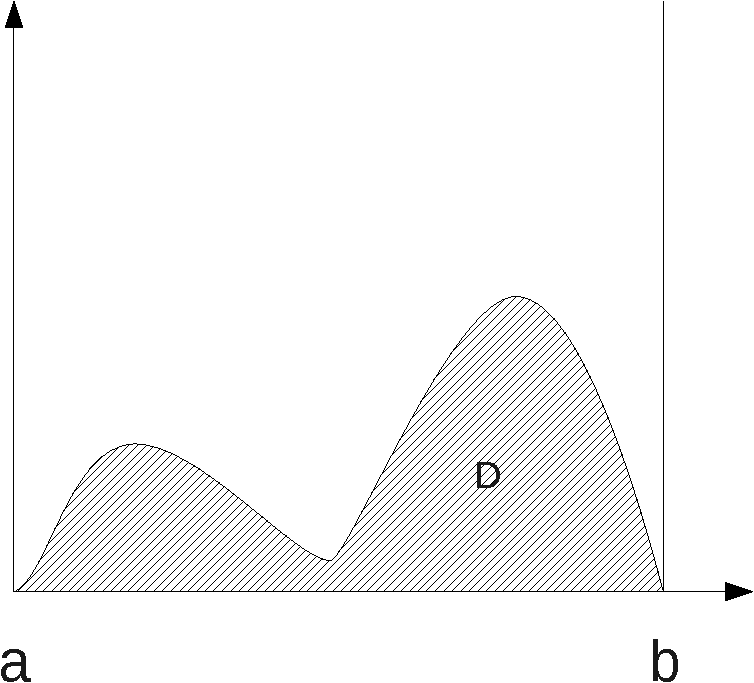
\includegraphics[scale=0.4]{images/surface_graphe.pdf}
\caption{Aire définie par un graphe d'application}\label{fig:01_01}
\end{figure}
L'aire de $\mathcal{D}$ peut être estimée en effectuant un découpage en
morceaux géométriquement simples (i.e. pour lesquels une aire peut facilement
être calculée) puis en sommant les différentes valeurs obtenues. Deux types de
découpages simples correspondant à des tranches verticales (resp. horizontales)
sont reproduits sur les figures \ref{fig:01_02}.

\begin{figure}
\begin{tabular}{cc}
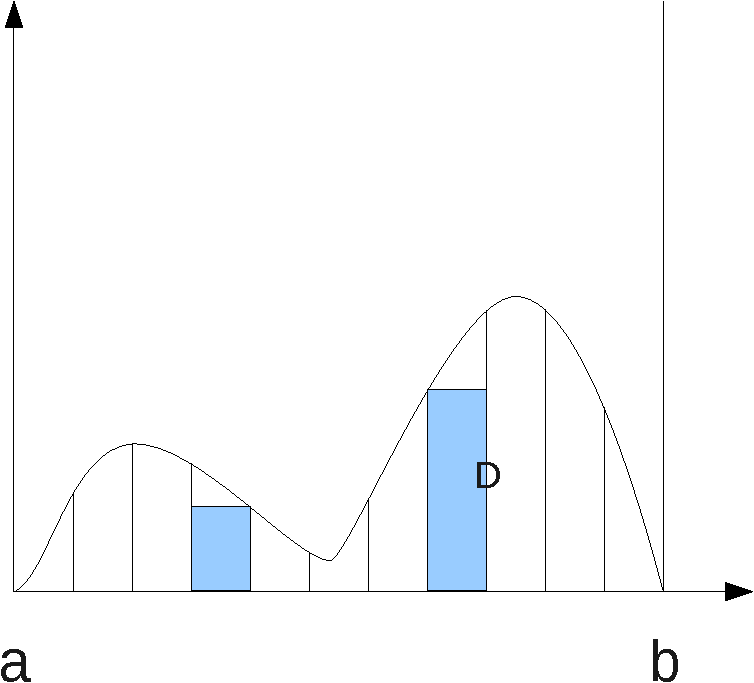
\includegraphics[scale=0.4]{images/graphe_riemann.pdf} & 
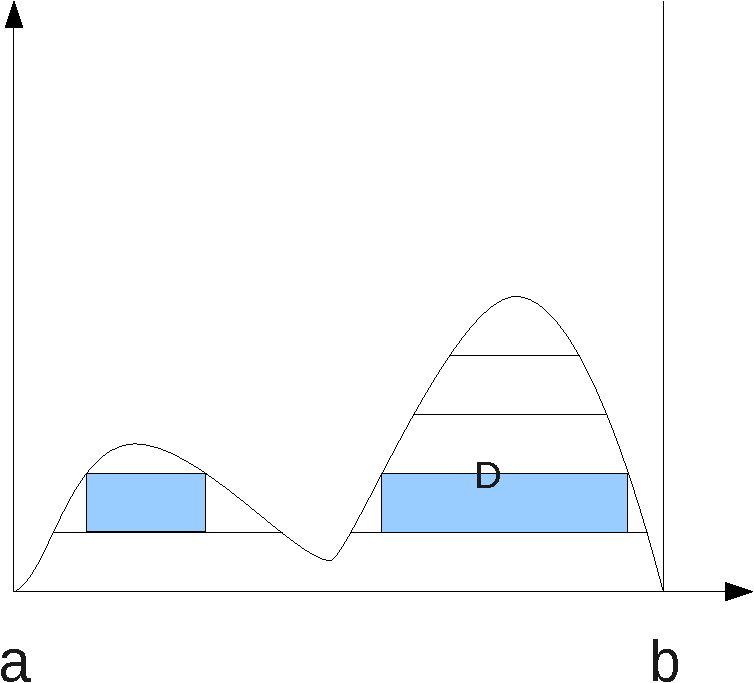
\includegraphics[scale=0.4]{images/graphe_lebesgue.pdf}
\end{tabular}
\caption{Découpages de Riemann et Lebesgue}\label{fig:01_02}
\end{figure}
Ces deux découpages vont correspondre dans la suite à deux notions
d'intégrales.

\subsection{Intégrale de Riemann}
L'estimation de la surface $\mathcal{D}$ à partir de bandes verticales est à la
base de la notion d'intégrale au sens de Riemann, qui est historiquement la
première à avoir été introduite. Ce découpage présente l'avantage considérable
de n'utiliser que des rectangles pour estimer l'aire de $\mathcal{D}$. Etant
donnée une subdivision $\mathcal{S}= \{ a = t_0 < t_1 < \dots < t_N = b \}$ de
l'intervalle $[a,b]$, et des points $\xi_i \in [t_i, t_{i+1}[, i = 0, \dots
,N-1$, une estimation de l'aire de $\mathcal{D}$ s'obtient à partir de
rectangles de base $[t_i, t_{i+1}]$ et de hauteur $f(\xi_i)$ comme:
\[
\mathcal{I}(\mathcal{S}, (\xi_i), f) =\sum_{i=0}^{N-1}
f(\xi_i)(t_{i+1}-t_i) \] $\mathcal{I}(\mathcal{S}, (\xi_i), f)$ est appelé somme
de Riemann de $f$ relative à la subdivision $\mathcal{S}$. Pour une subdivision
$\{ a = t_0 < t_1 < \dots < t_N = b \}$ donnée, les différentes sommes de Riemann
possibles différent par le choix des points d'évaluation $\xi_i, i=0 \dots N-1$.
Afin de pouvoir dégager une notion d'aire, il faut s'assurer de l'existence
d'une valeur limite aux sommes de Riemmann. La situation est un peu plus
compliquée que dans le cas des suites, l'ensemble des subdivisions sur un
intervalle donné n'étant pas dénombrable. La notion de filtre permet de
contourner le problème de façon élégante, mais on peut ici recourir à un
traitement plus simple. 
\begin{defn}
Soient  $\mathcal{S}_1= \{ a = t_0 < t_1 < \dots < t_N =
b \}$  et $\mathcal{S}_2= \{ a = u_0 < u_1 < \dots < u_M =
b \}$ deux subdivisions de $[a,b]$. On dira que $\mathcal{S}_2$ est plus fine
que $\mathcal{S}_1$, que l'on notera $\mathcal{S}_1 \prec \mathcal{S}_2$, si
$\mathcal{S}_1 \subset \mathcal{S}_2$.
\end{defn}

\begin{prop}\label{prop:union_subdivisions}
Pour tout couple de subdivisions $(\mathcal{S}_1,\mathcal{S}_2)$ de $[a,b]$, il
existe une subdivision $\mathcal{S}$ telle que $\mathcal{S}_1 \prec \mathcal{S}$
et $\mathcal{S}_2 \prec \mathcal{S}$
\end{prop}
\begin{proof}
Il suffit de poser $\mathcal{S}=\mathcal{S}_1 \cup \mathcal{S}_2$
\end{proof}

\begin{defn}\label{def:lim_riemann}
On dira que les sommes de Riemann de $f$ convergent vers une limite $l$ si pour
tout $\epsilon > 0$ il existe une subdivision $\mathcal{S}_{\epsilon}$ telle que
pour toute subdivision $\mathcal{S}=\{ a = t_0 < t_1 < \dots < t_N =
b \}$ plus fine que $\mathcal{S}_{\epsilon}$ et toute suite de points $\xi_i \in
[t_i, t_{i+1}[, \, i=0 \dots N-1$:
\[
|\mathcal{I}(\mathcal{S}, (\xi_i), f)-l| < \epsilon
\]
\end{defn}
La limite ainsi définie est unique. Supposons en effet l'existence d'une autre
valeur limite $l^\prime$ vérifiant la même propriété. Soit $\epsilon > 0$. Il
existe une subdivision $\mathcal{S}$ et une subdivision $\mathcal{S}^\prime$
telles que $|\mathcal{I}(\mathcal{S}, (\xi_i), f)-l| < \epsilon$,
$|\mathcal{I}(\mathcal{S^\prime}, (\xi^\prime_i), f)-l^\prime| < \epsilon$, les
mêmes inégalités étant vérifiées par toute subdivision plus fine. Par la
proposition \ref{prop:union_subdivisions}, il existe une subdivision
$\mathcal{U}$ plus fine que $\mathcal{S}$ et $\mathcal{S}^\prime$. Toute somme
de Riemann $\mathcal{I}(\mathcal{U}, (\theta_i), f)$ associée à $\mathcal{U}$
verifiera:
\[
|\mathcal{I}(\mathcal{U}, (\theta_i), f)-l| < \epsilon, \quad
|\mathcal{I}(\mathcal{U}, (\theta_i), f)-l^\prime| < \epsilon
\]
L'inégalité triangulaire montre alors que $|l-l^\prime|<2\epsilon$ et comme ceci
est vrai pour tout $\epsilon >0$, on en déduit $l=l^\prime$.
Le critère de Cauchy s'étend à la notion de limite indexée par des subdivisions. 
Enfin, si l'on se donne une subdivision $\mathcal{S}=\{ a = t_0 < t_1 < \dots <
t_N = b \}$, la quantité $\delta_{\mathcal{S}} = \sup \{ t_{i+1}-t_i, \,
i=0\dots N-1$ est appelée pas de $\mathcal{S}$. Si $\mathcal{S} \prec
\mathcal{S}^\prime$, alors $\delta_{\mathcal{S}^\prime} < \delta_{\mathcal{S}}$.
De plus, en choisissant des subdivisions de plus en plus fines, on peut faire
tendre le pas vers 0: ceci justifie l'abbréviation ''lorsque le pas des
subdivisions tend vers 0'' pour décrire la convergence des sommes de Riemann.

La valeur limite $l$ dans la définition \ref{def:lim_riemann}, lorsqu'elle
existe, est l'intégrale de Riemann de $f$ sur l'intervalle $[a,b]$ que l'on note
conventionnellement $\int_a^b f(t)dt$. Le point critique pour l'intégrabilité au
sens de Riemann est l'indépendance du choix des points $\xi_i$:
ceci impose une condition relativement forte sur le comportement local des
applications, comme le montre la proposition suivante.
\begin{prop} 
Soit $f \colon [a,b] \to \mathbb{R}^+$ telle qu'en tout
point de $]a,b[$, $f$ admette une limite à droite et à gauche, ainsi qu'une
limite à gauche (resp. à droite) en $b$ (resp. $a$). Alors $f$ est intégrable au
sens de Riemann.
 \end{prop}
 \begin{proof}
 L'idée de la preuve est résumée sur la figure \ref{fig:01_04}. Soit
 $\epsilon > 0$. Pour tout $t \in [a,b]$, il existe un intervalle ouvert
 (pour la topologie induite) $V_t = [a,b] \cap ]t-\eta_1, t+\eta_2[$  tel que
 $\forall x \in V_t, x < t$ (resp. $\forall x \in V_t, x > t$), $|f(x)
 -f(t^-)|<\epsilon$ (resp. $|f(x)-f(t^+)|<\epsilon$). L'intervalle $[a,b]$ étant compact, 
 un nombre fini de ces ouverts le recouvre ; on les notera $V_{t_i}, i = 0,
 \dots, N$.  Sans perte de généralité, on supposera que chaque intervalle
 contient un unique point $t_i$ de la subdivision et on posera $\theta = \inf \{
 t_{i+1}-t_i, i=0, \dots, N-1 \}$ . On peut déduire de l'écriture précédente l'existence d'une borne pour $f$, i.e. $\exists M >0, \, \forall x \in [a,b],
 |f(x)|\leq M$. Soient deux subdivisions $\mathcal{S}_1=\{x_0 < \dots <
 x_{N_1}\}$, $\mathcal{S}_2 = \{ y_0 < \dots < y_{N_2} \}$ de pas inférieur à
 $\theta$ et deux suites de points $(\xi_i)_{i=0, \dots, N_1 -1}$,
 $(\xi_j^\prime)_{j=0, \dots, N_2-1}$ vérifiant $\forall i=0, \dots, N_1-1,
 \xi_i \in [x_i, x_{i+1}[$ (resp. $\forall j=0, \dots, N_2-1,
 \xi_j^\prime \in [y_j, y_{j+1}[$). On posera $(z_k)_{k=0, \dots, N_3}$ la
 suite ordonnée obtenue à partir de l'ensemble $\{x_i,y_j, \,
 i=0,\dots,N_1 \,,  j=0, \dots, N_2 \}$ et $(\eta_k)_{k=0,\dots,N_3}$ (resp.
 $(\eta_k^\prime)_{k=0,\dots,N_3}$) la suite telle que $\eta_k = \xi_i \text{ si
 } [z_k, z_{k+1}[ \subset [x_i, x_{i+1}[$ (resp. $\eta_k^\prime = \xi_j^\prime
 \text{ si } [z_k, z_{k+1}[ \subset [y_j, y_{j+1}[$).
 On a:
 \begin{align*}
  & |\mathcal{I}(\mathcal{S}_1, (\xi_i), f) -\mathcal{I}(\mathcal{S}_2,
 (\xi^\prime_j), f)| = \\
 & \left|\sum_{i=0}^{N_1-1} f(\xi_i)(x_{i+1}-x_i) -
 \sum_{j=0}^{N_2-1}f(\xi_j^\prime)(y_{j+1}-y_j) \right| \leq \\
 & \sum_{k=0}^{N_3} |f(\eta_k)-f(\eta_k^\prime)|(z_{k+1}-z_k)
 \end{align*}
 Dans cette dernière somme, il existe $N$ indices $k$ tels que l'intervalle
 correspondant $[z_k, z_{k+1}[$ contienne exactement un des points $(t_i)_{i=0,
 \dots, N}$. Le terme correspondant se majore par $2Mh$ où
 $h=\sup(\delta(\mathcal{S}_1),\delta(\mathcal{S}_1))$. Pour tous les autres
 termes, $|f(\eta_k)-f(\eta_k^\prime)| < 2\epsilon$, ce qui donne au total la
 majoration:
 \[
 |\mathcal{I}(\mathcal{S}_1, (\xi_i), f) -\mathcal{I}(\mathcal{S}_2,
 (\xi^\prime_j), f)| \leq 2MNh + 2\epsilon(b-a)
 \]
 Si $h < \epsilon / N$, on obtient finalement:
  \[
 |\mathcal{I}(\mathcal{S}_1, (\xi_i), f) -\mathcal{I}(\mathcal{S}_2,
 (\xi^\prime_j), f)| \leq 2\epsilon(M +(b-a))
 \]
 ce qui montre que l'écart entre $\mathcal{I}(\mathcal{S}_1, (\xi_i), f)$ et $\mathcal{I}(\mathcal{S}_2,
 (\xi^\prime_j), f)$ peut être rendu aussi petit que l'on veut, indépendamment
 du choix des points $(\xi_i),(\xi_j^\prime)$, dès lors que les pas des
 subdivisions sont inférieurs à une valeur donnée. En vertu du critère de
 Cauchy, ceci implique l'existence de l'intégrale de Riemann de $f$.
 \end{proof}
 \begin{figure}
 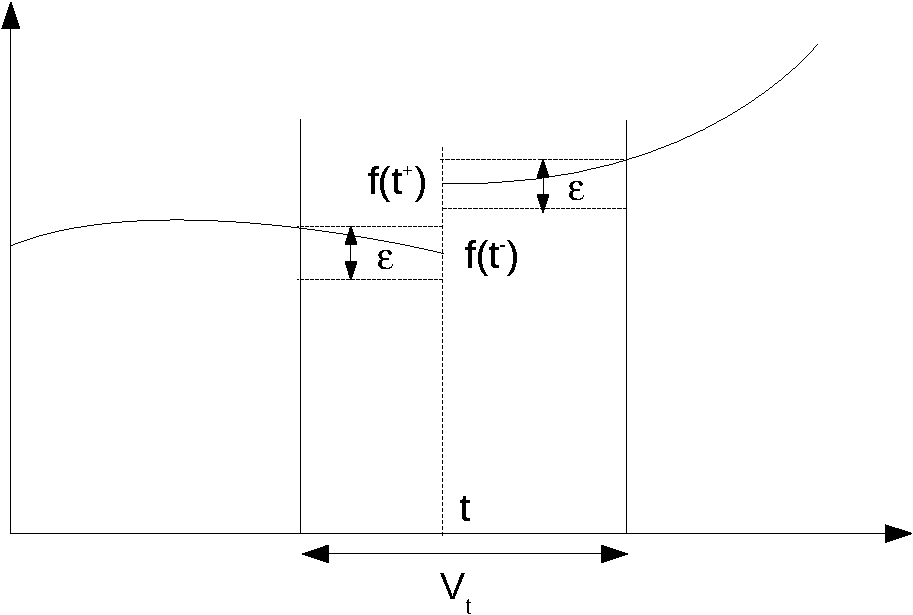
\includegraphics[scale=0.4]{images/fct_reglee.pdf}
 \caption{Encadrement de $f$ au voisinage d'un point $t$}\label{fig:01_04}
 \end{figure}
La preuve précédente dépend de façon critique du caractère compact de
l'intervalle $[a,b]$. L'extension à des domaines plus généraux ne pourra pas se
faire en utilisant le même procédé. De plus, on peut noter que la démonstration
qui vient d'être faite montre également que si une application $f$ vérifie les
hypothèse de la proposition, alors elle est limite uniforme d'applications en
escalier, qui sont définies comme suit:
\begin{defn}
Soit $[a,b]$ un intervalle compact. Une application $f \colon [a,b] \to
\mathbb{R}$ est dite en escalier si il existe une subdivision $a=t_0 < \dots <
t_N =b$ de $[a,b]$ telle que $f$ soit constante sur les intervalles
$]t_i,t_{i+1}[, i=0,\dots,N$.
\end{defn}
Ce qui implique aussi que $f$ ne peut avoir plus d'un nombre dénombrable de
points de discontinuité. 
On remarquera enfin, toujours en considérant la preuve effectuée, que
l'extension de l'intégrale de Riemann à des fonctions prenant leurs valeurs dans
un autre ensemble que $\mathbb{R}^+$ ne pose pas de problème dès lors qu'il
s'agit d'un espace topologique complet. Ceci explique pourquoi cette définition
de l'intégrale reste très utilisée. 

La difficulté majeure qui se pose avec l'intégration au sens de Riemann, et qui
a motivé en partie les travaux de Lebesgue, est la difficulté d'intervertir
limite et intégrale:
\begin{prop}
Soit $(f_n)_{n \in \mathbb{N}}$ une suite d'applications intégrables au sens de
Riemann et de limite uniforme $f$. Alors $f$ est intégrable au sens de Riemann
et:
\[
\int_a^b f(t) dt = \lim_{n \to +\infty} \int_a^b f_n(t)dt
\]
\end{prop}
\begin{proof}
Soit $\epsilon > 0$. Il existe $N_\epsilon \in \mathbb{N}$ tel que $\forall n
\geq  N_\epsilon$, $\sup_{x\in[a,b]} \left|f_n(x)-f(x)\right|<\epsilon$. Soit
$a=t_0<\dots<t_N=b$ une subdivision de $[a,b]$ et $(\xi_i)_{i=0,\dots, N-1}$ une
suite de points telle que $\xi_i \in [t_i,t_{i+1}[,i=0,\dots,N-1$. On a, pour
$n \geq N_\epsilon$:
\begin{align*}
& \left|\sum_{i=0}^{N-1}f(\xi_i)(t_{i+1}-t_i) -
\sum_{i=0}^{N-1}f_n(\xi_i)(t_{i+1}-t_i)\right|\\
& \leq
\sum_{i=0}^{N-1}\left|f(\xi_i)-f_n(\xi_i)\right|(t_{i+1}-t_i) \\
& \leq \epsilon(b-a)
\end{align*}
On en déduit que pour deux subdivisions $\mathcal{S}_1$, $\mathcal{S}_2$ et
deux suites associées $(\xi_i), (\xi_j^\prime)$:
\begin{align*}
& |\mathcal{I}(\mathcal{S}_1, (\xi_i), f) -\mathcal{I}(\mathcal{S}_2,
 (\xi^\prime_j), f) | \leq \\
 & |\mathcal{I}(\mathcal{S}_1, (\xi_i), f_n)
 -\mathcal{I}(\mathcal{S}_2, (\xi^\prime_j), f_n) | + 2 \epsilon (b-a)
\end{align*}
$f_n$ étant par hypothèse Riemann-intégrable, on a pour des subdivisions de
pas suffisamment petit:
\[
|\mathcal{I}(\mathcal{S}_1, (\xi_i), f) -\mathcal{I}(\mathcal{S}_2,
 (\xi^\prime_j), f) | \leq \epsilon(1 + 2 (b-a))
\]
En application du critère de Cauchy, on en déduit l'existence d'une limite à
$\mathcal{I}(\mathcal{S}, (\xi_i), f)$ lorsque le pas de la subdivision
$\mathcal{S}$ tend vers 0. L'égalité:
\[
\int_a^b f(t)dt = \lim_{n \to +\infty} \int_a^b f_n(t)dt
\]
s'obtient aisément.
\end{proof}
Il apparaît clairement dans cette preuve la nécessité de la convergence uniforme
afin de borner la différence entre une somme de Riemann de $f$ et de celle
de l'une des $f_n$: la convergence simple ne permet pas de conclure. 
Ce résultat montre également qu'il est possible de calculer l'intégrale de
Riemann d'une application à partir de la limite uniforme d'une suite
d'applications en escalier (voir plus haut). 

L'impossibilité de prendre une hypothèse plus faible que la convergence uniforme
résulte du découpage en tranches verticales choisi: il est nécessaire de
contrôler la hauteur du découpage, donc la valeur des fonctions sur tout un
intervalle. 

\subsection{Intégrale de Lebesgue}
Le second type de découpage definit par passage à la limite l'intégrale de
Lebesgue. Etant donné que les subdivisions effectuées se font sur l'ensemble des
valeurs de l'application, l'extension à des domaines généraux est relativement
aisée. De plus, pour la même raison, il ne sera pas nécessaire d'avoir
convergence uniforme pour conclure que l'intégrale d'une limite est la limite
des intégrales. La difficulté principale dans cette procédure réside dans le
fait qu'il est nécessaire de pouvoir définir la longueur d'une image réciproque
d'intervalle, qui n'a aucune raison d'être un intervalle. La définition précise
de cette longueur généralisée est l'objet de la théorie de la mesure. On
supposera que l'on dispose d'une telle "longueur" qui à une partie $A \subset
\mathbb{R}$ associe un réel positif $\lambda(A)$. Soit $f\colon \mathbb{R}\to
 \mathbb{R}^+$ une application à valeurs positives. Soit $a>0$ fixé et $0=t_0 <
\dots < t_N = a$ une subdivision de l'intervalle $[0,a]$. Une estimation par
défaut de l'aire sous-tendue au graphe de $f$ est obtenue facilement par:
\[
\sum_{i=0}^{N-1} t_{i} \lambda(f^{-1}([t_i, t_{i+1}[)) + t_N
\lambda(f^{-1}([a, +\infty[))
\]
Si le  passage à la limite $a \to +\infty$, $N \to \infty$ est possible, la
valeur ainsi obtenue sera appelée intégrale de Lebesgue. On peut se poser la
question de l'existence de la limite en question et de savoir si la définition 
de la surface au sens de Lebesgue est compatible, au
moins sur une classe assez large de fonctions, avec l'intégrale de Riemann
précédente. 
En guise de préliminaire assez intuitif, il para\^{\i}t raisonnable d'imposer
que pour un intervalle $[a,b[$, la longueur $\lambda([a,b[)$ soit $b-a$. Ceci
permet d'ores et déjà le calcul de l'intégrale de Lesbesgue sur des fonctions en
escalier. Soit $f \colon [a,b] \to \mathbb{R}^+$ une telle application qui
admettra une expression:
\[
f = \sum_{i=0}^N a_i 1_{I_i}
\]
avec $I_i$ un intervalle $[c_i, c_{i+1}[$.
On note de façon usuelle $1_A$ pour une partie $A \subset \mathbb{R}$
l'application indicatrice de $A$:
\[
f \colon x \mapsto \left \{
\begin{array}{cc}
0 & x \notin A \\
1 & x \in A
\end{array} 
\right.
\]

$f$ prend ses valeurs dans le compact $[0,
\sup_{i=0,\dots ,N}a_i]$. Soit $a > \sup_{i=0,\dots ,N}a_i$ et $0 = t_0 < \dots
< t_M = a$ une subdivision de l'intervalle $[0,a]$ de pas inférieur à $\inf
\{a_{i+1}-a_i, \, i=0, \dots, N-1\}$. Tout intervalle de la subdivision contient
soit aucun soit un unique point $a_i$. On en déduit que pour tout $t_j$,
$f^{-1}([t_j, t_{j+1}[)$ est soit vide (donc de longueur nulle), soit une union
disjointes des intervalles associés à l'unique valeur $a_i$ qui se trouve dans l'intervalle $[t_j, t_{j+1}[$, ce qui donne: 
\[
\sum_{i=0}^{N-1} t_{i} \lambda(f^{-1}([t_i, t_{i+1}[)) + t_N
\lambda(f^{-1}([a, +\infty[)) = \sum_{i=0}^N a_i (c_{i+1} - c_i)
\]
Cette expression est la même que celle trouvée dans le cadre de la théorie de
Riemann et laisse à penser que les deux notions d'intégrales coïncideront au
minimum sur les applications continues (une telle application étant limite
uniforme d'applications en escalier).

Les rapides développements précédents montrent au moins intuitivement que la
définition de l'intégrale de Lebesgue sera particulièrement simple, toute la
difficulté étant reportée sur la notion de "longueur" qui sera dans la suite
appelée mesure, et sur la détermination des parties pouvant admettre une mesure.
\section{Algèbres et tribus de parties}
Les notions d'algèbres et de tribus de parties sont à la base de
la théorie de la mesure.
\begin{mandatory}
\begin{defn}
Soit $E$ un ensemble. Un ensemble de parties $\mathcal{T}$ de $E$ est
appelé algèbre de parties si les axiomes suivants sont vérifiés~:
\begin{itemize}
\item $E \in \mathcal{T}$.
\item $A \in \mathcal{T} \Rightarrow A^c \in \mathcal{T}$ où la
  notation $A^c$ désigne le complémentaire de $A$ dans $E$.
\item Pour tout suite finie $(A_i)_{i=0\dots n}$ d'éléments de
  $\mathcal{T}$, $\cap_{i=0\dots n }  A_i \in \mathcal{T}$.
\end{itemize}
\end{defn}
\end{mandatory}
On notera que les axiomes précédents impliquent également que
$\emptyset \in \mathcal{T}$ et que toute union finie d'éléments de
$\mathcal{T}$ est encore un élément de $\mathcal{T}$.

\begin{mandatory}
\begin{defn}
Soit $E$ un ensemble. Une tribu $\mathcal{T}$ est un
ensemble de parties de $E$ vérifiant les axiomes~:
\begin{itemize}
\item $E \in \mathcal{T}$.
\item $A \in \mathcal{T} \Rightarrow A^c \in \mathcal{T}$ où la
  notation $A^c$ désigne le complémentaire de $A$ dans $E$.
\item Pour tout suite dénombrable $(A_i)_{i \in \mathbb{N}}$ d'éléments de
  $\mathcal{T}$, $\cap_{i \in \mathbb{N}}  A_i \in \mathcal{T}$.
\end{itemize}
\end{defn}
\end{mandatory}
Toute tribu est une algèbre~: il suffit de  remarquer que le dernier
axiome peut aussi s'appliquer aux familles finies $(A_i)_{0=1\dots n}$
en considérant une suite stationnaire $(B_i)_{i  \in \mathbb{N}}$~:
\[
B_i = \left \{ \begin{array}{cc}
A_i & i \leq n \\
A_n & i > n
\end{array} \right .
\]
\begin{term}
  Une tribu de parties est aussi appelée $\sigma$-algèbre de
parties (la lettre $\sigma$ préfixant un objet indique généralement une
extension des lois définies sur cet objet à des famillles dénombrables). Les
parties d'une tribu $\mathcal{T}$ sont appelées parties $\mathcal{T}$-mesurables.
\end{term}
\begin{exemple}
Pour tout ensemble $E$, l'ensemble des parties de $E$ forme de façon
évidente une tribu, de même que $\{E, \emptyset\}$. Ces
tribus sont respectivement, au sens de l'inclusion,  la plus grande et la plus petite tribu qui puisse se
construire sur $E$.
\end{exemple}
\begin{exemple}
Dans un ensemble $E$, l'ensemble des parties dénomb\-rables ou de
complémentaire dénombrable est également une tribu. Pour
vérifier ceci, seul l'axiome concernant les intersections ou
réunions dénombrables mérite examen. Soit $(A_i)_{i \in \mathbb{N}}$
une famille de parties mesurables. Pour tout $i \in \mathbb{N}$, $A_i$
ou $A_i^c$ est dénombrable. Supposons dans un premier temps qu'il
existe un entier $i_0$ tel que $A_{i_0}$ soit dénombrable. Comme
$\cap_{i \in \mathbb{N}} A_i \subset A_{i_0}$, on en déduit que le
cardinal de l'intersection est dénombrable. Si on ne peut trouver de
$i_0$ vérifiant la propriété, alors tous les $A_i^c$ sont de cardinal
dénombrable. $\cup_{i \in \mathbb{N}} A_i^c$ est aussi dénombrable. Comme par
ailleurs $\cap_{i \in \mathbb{N}} A_i = \left (\cup_{i \in \mathbb{N}}
A_i^c \right ) ^c$, $\cap_{i \in \mathbb{N}} A_i$ est de
complémentaire dénombrable, ce qui termine la démonstration.
\end{exemple}
\begin{exemple}
Dans un ensemble $E$ de cardinal infini, l'ensemble des parties
de cardinal fini ou de complémentaire de cardinal fini forme une
algèbre de parties, mais n'est pas une tribu~: comme $E$
est de cardinal infini, il est possible de choisir une famille
dénombrable 
$(x_i)_{i \mathbb{N}}$ d'éléments distincts. La réunion $\cup_{i
\in \mathbb{N}} \{ x_i \}$ est une réunion dénombrable de parties de
cardinal fini mais n'est pas elle même de cardinal fini. Comme par
ailleurs il est possible de faire une partition de $E$ sous la forme
de deux ensembles infinis (considérer par exemple $E=\mathbb{N}$ et
les entiers pairs et impairs), on peut faire en sorte que le cardinal
de son complémentaire ne soit pas non plus fini. 
\end{exemple}
\begin{prop}
Soit $\mathcal{T}$ une algèbre de parties sur un ensemble $E$. Si pour toute
famille $(A_i)_{i \in \mathbb{N}}$ d'éléments de $\mathcal{T}$, croissante au
sens de l'inclusion, on a $\cup_{i \in \mathbb{N}} A_i \in \mathcal{T}$
alors $\mathcal{T}$ est une tribu. La proposition subsiste
si l'on remplace famille croissante par famille décroissante et
réunion par intersection.
\end{prop}
\begin{proof}
Il suffit de vérifier l'axiome relatif aux unions dénombrables. Soit
$(A_i)_{i \in \mathbb{N}}$ une famille d'éléments de $\mathcal{T}$. La
famille $B_n = \cup_{i=0}^n A_i$ est croissante au sens de
l'inclusion. $\mathcal{T}$ étant une algèbre par hypothèse, $B_n \in
\mathcal{T}$ pour tout entier $n$, d'où $\cup_{i \in \mathbb{N}} B_i =
\cup_{i \in \mathbb{N}} A_i \in \mathcal{T}$.
La proposition relative aux familles décroissantes s'obtient par
passage au complémentaire.
\end{proof}
\begin{rem}
Il est possible de trouver d'autres caractérisations équivalentes des
tribus. En particulier, si l'on impose à une algèbre
$\mathcal{T}$ d'être stable par union dénombrable {\em disjointe},
$\mathcal{T}$ est une tribu. En effet, si $(A_i)_{i \in
\mathbb{N}}$ est une famille disjointe d'éléments de $\mathcal{T}$, la
famille $B_n =  \cup_{i=0 \dots n} A_i$ est une famille croissante au
sens de l'inclusion d'éléments de $\mathcal{T}$ et la proposition
précédente s'applique. 
\end{rem}
\begin{mandatory}
\begin{prop}Soit $E$ un ensemble. Toute intersection de
  tribus sur $E$ est encore une tribu sur $E$.
\end{prop}
\end{mandatory}
\begin{proof}
$E$ appartient à l'intersection des tribus car il appartient par définition
à chacune des tribus. Soit $A$ une partie de l'intersection. $A$ appartient à toutes
les tribus de l'intersection. $A^c$ appartient aussi à toutes les tribus
de l'intersection, donc à l'intersection. Enfin, si $(A_i)_{i \in \mathbb{N}}$ est une famille de parties
appartenant chacune à l'intersection des tribus, $\cap_{i \in \mathbb{N}} A_i$ appartient à toutes
les tribus et donc à l'intersection.
\end{proof}
\leftline{\em Attention !}
La réunion d'algèbres n'est pas nécessairement une algèbre comme le
montre l'exemple ci dessous avec $E= \{ 0, 1, 2 \}$~:
\begin{align*}
&\mathcal{T}_1 = \{ \emptyset, \{ 0,1 \}, \{ 2\}, E \} \\
&\mathcal{T}_2 = \{ \emptyset, \{ 0\}, \{1, 2\}, E \} \\
& \mathcal{T}_1 \cup \mathcal{T}_2 = \{ \emptyset, \{ 0\}, \{ 2\},  \{ 0,1
\},\{1, 2\}, E \}
\end{align*}
$\mathcal{T}_1, \mathcal{T}_2$ sont des algèbres, mais $ \mathcal{T}_1
\cup \mathcal{T}_2$ ne contient pas $\{1\} = \{ 0,1 \} \cap \{1, 2\}$
et ne peut donc être une algèbre.

On notera le très important corollaire suivant~:
\begin{mandatory}
\begin{corollaire}
Soit $E$ un ensemble et $\mathcal{F}$ un ensemble de parties de
$E$. Il existe une unique plus petite tribu contenant
$\mathcal{F}$, appelée tribu engendrée par $\mathcal{F}$.
\end{corollaire}
\end{mandatory}
L'ensemble des tribus contenant $\mathcal{F}$ n'est pas
vide car $\mathcal{P}(E)$ est une tribu.
Il suffit alors de construire l'intersection de toutes les
tribus contenant $\mathcal{F}$, qui est une
tribu par le corollaire précédent. L'unicité provient de la
minimalité de la tribu engendrée. 
La tribu engendrée par $\mathcal{F}$ sera notée $\sigma(\mathcal{F})$.
\begin{mandatory}
\begin{defn}
Soit $E$ un ensemble muni d'une topologie $\mathcal{O}$. La plus
petite tribu sur $E$ contenant les ouverts de $
\mathcal{O}$ est appelée tribu de Borel relativement à la
topologie $\mathcal{O}$.
\end{defn}
\end{mandatory}
La tribu de Borel sur $E$ est notée $\mathcal{B}(E)$, la topologie
étant sous-entendue. La tribu de Borel sur $E$ est également engendrée
par les fermés. Les éléments de la tribu de Borel s'appellent les boréliens.
La tribu de Borel  sur $\mathbb{R}^n$ muni de
la topologie induite par la norme euclidienne est d'un usage constant
en théorie de l'intégration. Il existe plusieurs façons équivalentes
de la construire, esentiellement à partir d'ensembles de parties simples comme
va le montrer la proposition suivante.
\begin{mandatory}
\begin{prop}
 La tribu de Borel sur $\mathbb{R}^n$ muni de
la topologie induite par la norme euclidienne est égale à la tribu engendrée par l'une quelconque
des familles suivantes~:
\begin{itemize}
\item L'ensemble des ouverts (resp. fermés) de $\mathbb{R}^n$.
\item L'ensemble des demi-espaces de la forme~:
\[
H_{i,\lambda} = \{ (x_1, \dots x_n) | x_i < \lambda \} 
\]
avec $i \in 1 \dots n, \lambda \in \mathbb{R}$.
\item L'ensemble des rectangles~:
\[
\{ (x_1,\dots ,x_n) | a_i \leq  x_i < b_i, \, i=1\dots n \}
\]
\end{itemize}
\end{prop}
\end{mandatory}
\begin{proof}
Soit $\mathcal{B}_1$ la tribu engendrée par les
demi-espaces et $\mathcal{B}_2$ la tribu engendrée par les
rectangles. On a $\mathcal{B}_1 \subset \mathcal{B}(\mathcal{R}^n)$
car les demi-espaces sont des ouverts. Un rectangle quelconque pouvant
être obtenu par intersection finie de différences de demi-espa\-ces, on
en déduit que l'ensemble des rectangles est inclus dans
$\mathcal{B}_1$, et donc, par minimalité de la tribu engendrée, que
$\mathcal{B}_2 \subset \mathcal{B}_1$.
Enfin, soit $O$ un ouvert de $\mathbb{R}^n$. Il existe une famille
dénombrable $(x^{(i)}_{i \in \mathbb{N}})$ de points de $O$ et une famille
$(r_i)_{i \in \mathbb{N}}$ de réels positifs telles que~:
\[
O = \bigcup_{i \in \mathbb{N}} B(x^{(i)}, r_i)
\]
avec $B(x^{(i)}, r_i)$ boule ouverte de centre $x^{(i)}$ et de rayon
$r_i$. Les normes étant équivalentes sur $\mathbb{R}^n$, on 
choisira la norme sup:
$$\| x \| = sup_{i=1\dots n}
|x_i|$$
 pour laquelle les boules ouvertes sont des rectangles
ouverts. Comme par ailleurs~:
\begin{align*}
&\{ (x_1,\dots ,x_n) | a_i <  x_i < b_i, \, i=1\dots n \}  = \\
&\bigcup_{k \geq 1} \{ (x_1,\dots ,x_n) | a_i + \frac{1}{k} \leq  x_i < b_i, \,
i=1\dots n \}
\end{align*}
on peut obtenir $O$ par réunion dénombrable de rectangle
semi-ouverts. Ceci prouve que l'ensemble des ouverts est contenu dans
$\mathcal{B}_2$. Par ail\-leurs, on a de façon évidente $\mathcal{B}_1
\subset \mathcal{B}(\mathbb{R}^n)$, ce qui termine la proposition.
\end{proof}
\begin{exercice}
On se place dans l'ensemble des nombres entiers naturels $\mathbb{N}$. 
 \begin{itemize}
  \item Soit $n \in \mathbb{N}$ un entier fixé. Déterminer la tribu
  $\mathcal{T}_n$ engendrée par les singletons $\{0\},\{1\},\dots,\{n\}$.
  \item Montrer que pour tout $N \in \mathbb{N}$:
  \[
  	\bigcup_{n=0}^N \mathcal{T}_n
  \]
  est une tribu.
  \item Est-ce que:
    \[
  	\bigcup_{n=0}^{+\infty} \mathcal{T}_n
  \]
  est encore une tribu ?
\end{itemize}
\end{exercice}
\section{Mesures}
\subsection{La droite réelle achevée}
En théorie de la mesure, l'usage de la droite réelle complétée par les
points $\{+\infty, -\infty \}$ ou de la demi-droite achevée $[0,
+\infty]$ est courant. Dans ce paragraphe, les propriétés utiles de
ces objets vont être brièvement rappelées. Les démonstrations des
différentes propositions sont laissées au lecteur à titre d'exercice.
\begin{defn}
La droite réelle achevée, notée $\overline{\mathbb{R}}$, est l'ensemble
$\mathbb{R} \cup \{ -\infty, +\infty \}$ muni de la topologie
suivante~:
\begin{itemize}
\item Toute partie de $\overline{\mathbb{R}}$ ne contenant pas
$+\infty$ ou $-\infty$ est ouverte si et seulement si elle est ouverte
dans $\mathbb{R}$ muni de sa topologie usuelle.
\item Une partie de  $\overline{\mathbb{R}}$ est un voisinage de
$+\infty$ (resp. $-\infty$) si et seulement si elle contient un
intervalle de la forme $]A, +\infty] = \{+\infty\} \cup \{ x \in
\mathbb{R} | x > A \}$ (resp. $[-\infty, A[ = \{-\infty\} \cup \{ x \in
\mathbb{R} | x < A \}$).
\end{itemize}
\end{defn}
On munira $\overline{\mathbb{R}}$ des règles arithmétiques suivantes~:
\begin{itemize}
\item Les opérations entre éléments de $\mathbb{R}$ sont les
opérations usuelles.
\item Si $x \in \mathbb{R}$, $x+(+\infty) = (+\infty) + x = +\infty$,
$x+(-\infty) = (-\infty) + x = -\infty$.
\item Si $x \in \mathbb{R}, x > 0$, $x.(+\infty) = (+\infty).x = +\infty$,
$x.(-\infty) = (-\infty) . x = -\infty$.
\item  Si $x \in \mathbb{R}, x < 0$, $x.(+\infty) = (+\infty).x = -\infty$,
$x.(-\infty) = (-\infty) . x = +\infty$.
\item $(+\infty)+(+\infty) = +\infty$,  $(-\infty)+(-\infty) =
-\infty$.
\item $(+\infty).(+\infty) = +\infty$, $(-\infty).(-\infty) =
+\infty$, $(+\infty).(-\infty) = -\infty$, $0.(+\infty)=0.(-\infty)=0$.
\end{itemize}
Les opérations précédentes sont commutatives. La somme
$(+\infty)+(-\infty)$ n'est pas définie.
La valeur absolue de $\mathbb{R}$ se prolonge sur la droite achevée
par $|+\infty|=|-\infty|=+\infty$.
\begin{prop}
Toute partie $A \subset \overline{\mathbb{R}}$ admet une borne
supérieure notée $sup(A)$ et une borne inférieure notée $inf(A)$.
\end{prop}
La caractérisation suivante du $sup$ est très utile en pratique.
\begin{prop}
$\lambda \in \mathbb{R}$ est la borne supérieure de $A$ si~:
\begin{itemize}
\item $\forall x \in A, \, x \leq \lambda$.
\item $\forall \epsilon > 0, \exists y \in A | y > \lambda - \epsilon$.
\end{itemize}
$+\infty$ est la borne supérieure de $A$ si $\forall M \in
\mathbb{R}, \exists x \in A | x > M$. 
\end{prop}
Cette caractérisation se transpose de façon évidente à l'$inf$.
\begin{mandatory}
\begin{defn}
Soit $(x_n)_{n \in \mathbb{N}}$ une suite d'éléments de
$\overline{\mathbb{R}}$. La limite supérieure (resp. inférieure) de
cette suite, notée $\limsup_n x_n$ (resp. $\liminf_n x_n$), est~:
\[ \limsup_n x_n =\inf_{k \in \mathbb{N}} \sup_{n \geq k} x_n 
\]
resp.~:
\[ \liminf_n x_n = \sup_{k \in \mathbb{N}} \inf_{n \geq k} x_n
\]
 Une suite est dite convergente
si $\liminf_n = \limsup_n$ et la valeur commune est appelée limite de
la suite.
\end{defn}
\end{mandatory}
\begin{rem}
Les limites inférieure et supérieure, définies à partir des bornes
inférieures et supérieures existent toujours, contrairement à la
limite. Dans $\overline{\mathbb{R}}$, la limite d'une suite
convergente peut être $+\infty$ ou $-\infty$. On trouve quelquefois le
terme de suite divergente vers l'infini pour qualifier de telles suites.
\end{rem}
\subsection{Mesures positives}
\begin{defn}
Soit $E$ un ensemble et  $\mathcal{T}$ une tribu sur
$E$. Le couple $(E, \mathcal{T})$ est appelé espace mesurable. 
\end{defn}
\begin{mandatory}
\begin{defn}
Soit $(E, \mathcal{T})$ un espace mesurable. Une mesure sur cet espace
est une application $\mu : \mathcal{T} \to [0, +\infty]$ vérifiant~:
\begin{itemize}
\item $\mu(\emptyset) = 0$.
\item Pour toute suite $(A_i)_{i \in \mathbb{N}}$ d'éléments disjoints
  de  $\mathcal{T}$, on a~:
\[
\mu \left ( \cup_{i \in \mathbb{N}} A_i \right ) = \sum_{i
  =0}^{+\infty} \mu(A_i)
\]
\end{itemize}
\end{defn}
Le triplet $(E, \mathcal{T}, \mu)$ est appelé espace mesuré.
\end{mandatory} 

Voici quelques exemples de mesures usuelles~:
\begin{itemize}
\item Soit $E$ un ensemble muni de la tribu formée par l'ensemble des
  parties de $E$. La mesure définie par $\mu(A) = +\infty$ si $A$ est
  de cardinal infini et $\mu(A)= \#A$ sinon est appelée mesure de
  dénombrement.
\item Soit $(E, \mathcal{T})$ un espace mesurable et soit $x \in
  E$. On pose $\delta_x(A) = 0$ si $x \notin A$ et $\delta_x(A) = 1$
  sinon. La mesure obtenue est la mesure de Dirac (ou ponctuelle)
  centrée en $x$.
\end{itemize}
Une mesure très importante en pratique sera définie ultérieurement sur la tribu
de Borel de $\mathbb{R}$ et associera à un intervalle ouvert $]a,b[$ sa
longueur. La construction de cette mesure est néanmoins délicate et ne
pourra se faire qu'après un travail préliminaire assez long. 

\begin{defn}
Une mesure $\mu$ sur $(E, \mathcal{T})$ est dite finie si $\mu(E) <
+\infty$. Elle est dite $\sigma$-finie si il existe une famille
$(A_i)_{i \in \mathbb{N}}$ d'éléments de $\mathcal{T}$ telle que $E =
\cup_{i \in \mathbb{N}} A_i$ et $\forall n \in \mathbb{N}, \, \mu(A_n) < +\infty$.
\end{defn}
Une mesure $\mu$ finie telle que $\mu(E) = 1$ est appelée mesure de
probabilité. Un {\em atome} est un élément $x \in E$ tel que
$\{x\} \in \mathcal{T}, \, \mu(\{x\}) > 0$. Une mesure ne possédant
aucun atome est dite {\em diffuse} ou {\em continue}.
\begin{mandatory}
\begin{prop}\label{prop:1}
Soit $(E, \mathcal{T}, \mu)$ un espace mesuré. Soient $A,B$ deux
éléments de  $\mathcal{T}$ vérifiant $A \subset B$. On a $\mu(A) \leq
\mu(B)$. Si de plus $\mu(A) < +\infty$, $\mu(B-A) = \mu(B) - \mu(A)$.
\end{prop}
\end{mandatory}
\begin{proof}
$A$ et $B-A$ sont disjoints et $B = A \cup (B-A)$, on a donc $\mu(B) =
\mu(A) + \mu(B-A)$, d'où $\mu(B) \geq \mu(A)$. Si $\mu(A)< +\infty$, il est
possible de soustraire $\mu(A)$ aux deux membres de l'égalité, ce qui donne:
\[
\mu(B-A) = \mu(B) - \mu(A)
\]
\end{proof}
\begin{mandatory}
\begin{prop}
Soit $(E, \mathcal{T}, \mu)$ un espace mesuré. Pour toute suite
$(A_i)_{i \in \mathbb{N}}$ d'éléments de  $\mathcal{T}$, on a~:
\[
\mu \left ( \cup_{i \in \mathbb{N}} A_i \right ) \leq 
\sum_{i =0}^{+\infty} \mu(A_i)
\]
\end{prop}
\end{mandatory}
\begin{proof}
On pose $B_0 =A_0$ et pour tout $i > 0$, $B_i = A_i - \cup_{k=0}^{i-1}
A_k$. Les $B_i$ sont disjoints et $\cup_{i\in \mathbb{N}}B_i = \cup_{i
  \in \mathbb{N}} A_i$. On en déduit~:
\[
\mu(\cup_{i \in \mathbb{N}}A_i) = \mu(\cup_{i \in \mathbb{N}} B_i) =
\sum_{i = 0}^{+\infty} B_i
\] 
De plus, pour tout $i$, $B_i
\subset A_i$, donc $\mu(B_i) \leq \mu(A_i)$. On en déduit la proposition.
\end{proof}
\begin{mandatory}
\begin{prop}
Soit $(E, \mathcal{T}, \mu)$ un espace mesuré. Alors~:
\begin{itemize}
\item Si $(A_i)_{i \in \mathbb{N}}$ est une famille croissante
  d'éléments de  $\mathcal{T}$, alors~:
\[
\mu(\cup_{i \in \mathbb{N}} A_i) =
  \lim_{i \to +\infty}\mu(A_i)
\]
\item  Si $(A_i)_{i \in \mathbb{N}}$ est une famille décroissante
  d'éléments de  $\mathcal{T}$ et si il existe $n_0$ tel que
  $\mu(A_{n_0})<+\infty$, alors~:
\[
\mu(\cap_{i \in \mathbb{N}} A_i) =  \lim_{i
  \to +\infty} \mu(A_i)
\]
\end{itemize}
\end{prop}
\end{mandatory}
\begin{proof}
Soit $(A_i)_{i \in \mathbb{N}}$ une famille croissante d'éléments de
$\mathcal{T}$. On pose $B_0 = A_0$ et pour tout $i> 0$, $B_i = A_i -
A_{i-1}$. Les ensembles $B_i$ sont disjoints et vérifient $\cup_{i \in
  \mathbb{N}} A_i
= \cup_{i \in \mathbb{N}} B_i$. On en déduit que~:
\[
\mu \left ( \cup_{i \in \mathbb{N}} A_i \right ) = \sum_{i=0}^{+\infty} \mu(B_i) = \lim_{i \to +\infty} \mu \left (
\cup_{j=0}^i B_j \right ) = \lim_{i \to +\infty} \mu(A_i)
\] 
Soit maintenant $(A_i)_{i \in \mathbb{N}}$ une famille décroissante
d'éléments de $\mathcal{T}$. On peut, sans perte de généralité,
supposer que l'indice $n$ pour lequel $\mu(A_n) < +\infty$ est 0. Il
est clair, la famille $(A_i)$ étant décroissante, que pour tout $i \in
\mathbb{N}, \mu(A_i) < +\infty$. On pose, pour tout $i$, $C_i = A_0 - A_i$.
La famille $(C_i)$ est une famille croissante d'éléments de  $\mathcal{T}$. De
plus, $\cup_{i \in \mathbb{N}} C_i = A_0 - \cap_{k \in \mathbb{N}} A_k$. On a
donc, en utilisant le résultat ci-dessus~:
\[
\mu \left ( A_0 - \cap_{k \in \mathbb{N}} A_k \right) = \lim_{i \to +\infty} \mu(A_0 - A_i)
\]
Comme par hypothèse $\forall i \in \mathbb{N}, \mu(A_i) < +\infty$, on peut appliquer la
proposition \ref{prop:1} pour obtenir~$\mu(\cap_k A_k) = \lim_{i \to +\infty} A_i$.
\end{proof}
Une application $\mu$ définie sur  $\mathcal{T}$ et à valeurs dans
$[0,+\infty]$ est dite additive si, pour toute famille finie $(A_i)_{i=0\dots n}$ d'éléments disjoints de
$\mathcal{T}$,  elle vérifie~:
\[
\mu(\cup_{i=0\dots n} A_i) = \sum_{i=0}^n \mu(A_i)
\]
Toute mesure est une application additive, la réciproque étant
fausse. Cependant une application additive vérifiant certaines
hypothèses additionnelles est une mesure. En
particulier, on a~:
\begin{prop}\label{prop:2}
Soit $\mu$ une application additive définie sur un espace mesurable
$(E, \mathcal{T})$. $\mu$ est une mesure si l'une des hypothèses
suivantes est vérifiée.
\begin{itemize}
\item Pour toute famille croissante $(A_i)_{i \in \mathbb{N}}$ d'éléments de
  $\mathcal{T}$, on a~:
\[
\mu(\cup_{i \in \mathbb{N}}  A_i) = \lim_{i \to +\infty} \mu(A_i)
\]
\item Pour toute famille décroissante $(B_i)$ d'éléments de
  $\mathcal{T}$ vérifiant $\cap_{i \in \mathbb{N}} B_i = \emptyset$ on a~:
\[
\lim_{i\to +\infty} \mu(B_i) = 0
\]
\end{itemize}
\end{prop}
\begin{proof}
Soit $(B_k)_{k \in \mathbb{N}}$ une famille d'éléments disjoints de  $\mathcal{T}$. On
pose $A_i = \cup_{k=0}^i B_k$. Par l'additivité de $\mu$, on a
$\mu(A_i) = \sum_{k=0}^i \mu(B_k)$. Comme par ailleurs $\cup_{k \in
  \mathbb{N}} B_k = \cup_{i \in \mathbb{N}} A_i$, on vérifie aussi:
\[
\lim_{i \to +\infty} \mu\left(\bigcup_{k=0}^iB_k\right) = \lim_{i \to
+\infty} \mu(A_i)= \lim_{i \to +\infty} \sum_{k=0}^i \mu(B_k)
\]
qui prouve l'additivité pour des
familles dénombrables.
Supposons maintenant la deuxième hypothèse vérifiée et soit $A_k =
\cup_{i\geq k}B_i$. Alors, pour tout $j \in \mathbb{N}$~:
\[
\mu (\cup_{k\in \mathbb{N}} B_k) = \sum_{i=0}^j \mu(B_i) + \mu(A_{j+1})
\]
et finalement~:
\[
\mu(\cup_{k \in \mathbb{N}} B_k) = \lim_{j \to +\infty}  \sum_{i=0}^j \mu(B_i)
\]
\end{proof}

\begin{exercice}
Soit $(E, \mathcal{T}, \mu)$ un espace mesuré. Soit $(A_n)_{n  \in \mathbb{N}}$ une suite d'éléments de 
$\mathcal{T}$. On pose pour tout entier $k$~: $B_k = \cup_{i \geq k} A_i$.
\begin{itemize}
  \item  Montrer que la suite $(B_k)_{k \in \mathbb{N}}$ est décroissante au
  sens de l'inclusion. 
  \item Montrer que $\cap_{k \in \mathbb{N}} B_k$ est la partie de $E$ dont les
  éléments appartiennent à une infinité de $(A_i)_{i \in  \mathbb{N}}$.
  \item En déduire que si $\sum_{n \in \mathbb{N}} \mu(A_n) < +\infty$ alors la
mesure de l'ensemble des points de $E$ appartenant à une infinité de $A_n$ est nulle.
\end{itemize}

\end{exercice}

\section{Mesures extérieures}
\subsection{Mesure de Lebesgue pour des ouverts}
La construction de mesures sur $\mathbb{R}$ et de tribus de parties
associées est une opération délicate. Même dans le cas en apparence élémentaire
de la longueur généralisée qui doit associer à un intervalle $[a,b[$ la valeur
$b-a$, la question de savoir quelles sont les parties de $\mathbb{R}$ qui vont
admettre une telle longueur est loin d'être triviale. Les axiomes des tribus
permettent cependant de se faire une idée de ce que peut être une telle mesure
 sur une classe de parties plus restreinte.

Supposons que l'on dispose
d'une tribu $\mathcal{T}$ contenant tous les intervalles $[a,b[$.
$\mathcal{T}$ doit également contenir tous les intervalles fermés $[a,b]$
(resp. ouverts $]a,b[$) car $[a,b] = \cap_{n \to +\infty} [a, b + n^{-1}[$
(resp. $]a,b[ = \cup_{n \to +\infty} [a + n^{-1}, b[$). De plus, en vertu de la
proposition \ref{prop:1}, la longueur de l'intervalle $[a,b]$ (resp. $]a,b[$)
reste égale à $b-a$. De même la longueur de l'intervalle $]a,b]$ devra être
$b-a$. On posera dans la suite $\lambda(I)$ la longueur de l'intervalle $I$.
Soit $I_i, i=1, \dots, N$ un ensemble fini d'intervalles. Toute intersection
d'intervalles étant un intervalle, $\lambda \left( \cap_{i=1,\dots,N}
I_i\right)$ est bien définie. De même, $\cup_{i=1, \dots, N} I_i$ peut s'écrire
sous la forme d'une union disjointe d'intervalles, ce qui permet de définir
$\lambda \left( \cup_{i=1,\dots,N} I_i\right)$.
Enfin, pour une union dénombrable d'intervalles $I_i, i\in \mathbb{N}$, la
proposition \ref{prop:1} permet d'obtenir:
\[
\lambda \left( \cup_{i \in
\mathbb{N}} I_i \right)  = \lim_{ N \to + \infty} \lambda \left( \cup_{i=1,
\dots, N} I_i \right)
\]
Un résultat classique de topologie montre que tout ouvert de $\mathbb{R}$ peut
s'écrire comme une union dénonbrable d'intervalles deux à deux disjoints: on
peut ainsi définir $\lambda(U)$ pour tout $U$ ouvert.

\subsection{Mesures extérieures}
Les axiomes des mesures permettent de définir $\lambda$ pour des ensembles
construits à partir d'opérations simples sur les intervalles. L'extension à des
ensembles plus généraux s'obtient à l'aide d'une construction due à Carathéodory
qui va être présentée ci-dessous.
\begin{mandatory}
\begin{defn}
Soit $E$ un ensemble et soit $\mathcal{P}(E)$ l'ensemble des parties
de $E$. Une mesure extérieure sur $E$ est une application~:
\[
\mu^* : \mathcal{P}(E) \to [0,+\infty]
\]
 vérifiant~:
\begin{itemize}
\item $\mu^*(\emptyset) = 0$.
\item Pour $A,B$ parties de $E$, $A \subset B \, \Rightarrow \mu^*(A)
  \leq \mu^*(B)$.
\item Pour toute famille dénombrable $(A_i)_{i \in \mathbb{N}}$ de parties de $E$~:
\[
\mu^*(\cup_{i \in \mathbb{N}} A_i) \leq \sum_{i=0}^{+\infty} \mu^*(A_i)
\]
\end{itemize}
\end{defn}
\end{mandatory}
Une mesure n'est pas en général une mesure extérieure, n'étant pas définie
pour toute partie mais seulement pour les éléments d'une
tribu. 

\begin{mandatory}
Si l'on se place dans $\mathbb{R}$, on peut définir la mesure
extérieure de Lebesgue $\lambda^*$ de la façon suivante~:

 Pour toute partie $A$ de $\mathbb{R}$, on
considère l'ensemble $R_A$ des suites de $(a_i,b_i)_{i \in
  \mathbb{N}}$ de $\mathbb{R}^2$ telles 
que $\forall i \in \mathbb{N}, a_i \leq  b_i$ et $A \subset \cup_{i \in \mathbb{N}} ]a_i, b_i[$. $R_A$ n'est pas
  vide car $A \subset \mathbb{R}  = \cup_{i \in \mathbb{N}} ]-i , i [$.
On pose~:
\[
\lambda^*(A) = \inf_{((a_i,b_i)_{i \in \mathbb{N}}) \in R_A} \sum_i (b_i-a_i)
\]
\end{mandatory}
\begin{exercice}
Montrer que pour tout singleton $\{x\}, x\in \mathbb{R}$, on a: 
\[
\lambda^*\left(\{x\}\right)=0
\]
\end{exercice}
\begin{prop}
$\lambda^*$ est une mesure extérieure.
\end{prop}
\begin{proof}
pour tout $\epsilon > 0$, on peut trouver un intervalle $]a,b[$ tel
que $b-a < \epsilon$. Un tel intervalle contient bien évidemment
$\emptyset$ et l'infimum pour $\epsilon \to 0$ des longueurs est 0. On en
déduit que $\lambda^*(\emptyset)= 0$. Si $A\subset B$, la propriété
$\lambda^*(A) \leq \lambda^*(B)$ est évidente, toute famille
d'intervalles couvrant $B$ couvrant également $A$. Enfin, soit une
famille dénombrable $(A_i)_{i \in \mathbb{N}}$. Si $\sum_{i=0}^{+\infty}
\lambda^*(A_i) = +\infty$ la propriété est évidente. Sinon, soit $\epsilon > 0$. Pour tout indice
$n \in \mathbb{N}$, on peut trouver une suite $(a_{n,i},b_{n,i})_{i
  \in \mathbb{N}}$ telle
que~:
\[
\sum_{i = 0}^{+\infty} (b_{n,i} - a_{n,i}) < \lambda^*(A_n) + \frac{\epsilon}{2^n}
\]
le résultat suit alors en sommant sur $n$ (la série en $\epsilon$ est
convergente).
\end{proof}
On vérifie facilement que la mesure extérieure de Lebesgue d'un
intervalle quelconque est sa longueur ($+\infty$ pour un intervalle non borné)
et coïncide avec $\lambda$ précédemment introduit.

On peut étendre facilement la mesure extérieure de Lebesgue au cas des rectangles
de $\mathbb{R}^n$, en associant à un rectangle son volume.

\begin{mandatory}
\begin{defn}
Soit $E$ un ensemble et $\mu^*$ une mesure extérieure sur $E$. On dit
qu'une partie $A$ de $E$ est mesurable pour $\mu^*$ si pour toute
partie $B$ de $E$ on a~:
\[
\mu^*(B) = \mu^*(A\cap B) + \mu^*(A^c \cap B)
\]
\end{defn}
\end{mandatory}
\begin{rem}
Il suffit de vérifier~:
\[
\mu^*(B) \geq \mu^*(A\cap B) + \mu^*(A^c \cap B)
\]
pour que $A$ soit mesurable, puisque~:
\[
\mu^*(B) \leq \mu^*(A\cap B) + \mu^*(A^c \cap B)
\]
est toujours vrai.
\end{rem}
\begin{prop}
Toute partie $A$ de $E$ vérifiant $\mu^*(A)=0$ ou $\mu^*(A^c)=0$ est
$\mu^*$-mesurable. 
\end{prop}
\begin{proof}
La proposition~:
\[
\mu^*(B) \geq \mu^*(A\cap B) + \mu^*(A^c \cap B)
\]
est évidente puisque par hypothèse l'un des deux termes de droite est nul.
\end{proof}
\begin{mandatory}
\begin{theorem}
Soit $E$ un ensemble et $\mu^*$ une mesure extérieure sur
$E$. L'ensemble des parties $\mu^*$-mesurables forme une tribu
$\mathcal{T}$ et
$\mu^*$ définit par restriction une mesure sur celle-ci.
\end{theorem}
\end{mandatory}
\begin{proof}
On remarque tout d'abord que si $A$ est mesurable, alors $A^c$ l'est
aussi (cf définition). Soit maintenant $A_1,A_2$ parties
mesurables. Pour toute partie $B$ de $E$, on a~:
\begin{align*}
& \mu^*(B\cap (A_1 \cup A_2)) = \\
&\mu^*(B\cap (A_1 \cup A_2) \cap A_1) +
\mu^*(B\cap (A_1 \cup A_2) \cap A_1^c) = \\
&  \mu^*(B \cap A_1) + \mu^*(B
\cap A_1^c \cap A_2)
\end{align*}
Par ailleurs, $(A_1 \cup A_2)^c = A_1^c \cap A_2^c$, d'où~:
\[
\mu^*(B\cap (A_1 \cup A_2)) + \mu^*(B\cap (A_1 \cup A_2)^c) = 
\mu^*(B\cap A_1) + \mu^*(B \cap A_1^c) = \mu^*(B) 
\]
d'où $A_1 \cup A_2$ est mesurable. 
Il reste à prouver la stabilité par union dénombrable, i.e. $\bigcup_{n \in
\mathbb{N}} A_n$ mesurable si les $A_n,n \in \mathbb{N}$ sont des parties
mesurables.  
Considérons dans un premier temps une famille de parties mesurables disjointes, $(A_i)_{i \in \mathbb{N}}$. 
Soit $B$ une partie de $E$. La
mesurabilité de $A_0$ donne~:
\[
\mu^*(B) = \mu^*(B\cap A_0)+ \mu^*(B \cap A_0^c)
\]
On va montrer par récurrence que pour tout entier $n$~:
\[
\mu^*(B) = \sum_{i=0}^n \mu^*(B \cap A_i) + \mu^*(B \cap \left (
\cap_{i=0}^n A_i^c \right ))
\]
On a~:
\begin{align*}
\mu^*(B \cap \left (
\cap_{i=0}^n A_i^c \right )) = & \mu^*(B\cap \left (
\cap_{i=0}^n A_i^c \right ) \cap A_{n+1}) + \\
&\mu^*(B \cap \left (
\cap_{i=0}^n A_i^c \right ) \cap A_{n+1}^c) \\
&=  \mu^*(B \cap A_{n+1}) + \mu^*(B \cap \left (
\cap_{i=0}^{n+1} A_i^c \right )) 
\end{align*}
La suite $(B \cap (\cap_{i=0}^n A_i^c))_{n \in \mathbb{N}}$ est
  décroissante au sens de l'inclusion, donc la suite $(\mu^*(B \cap 
  (\cap_{i=0}^n A_i^c)))_{n \in \mathbb{N}}$ est décroissante, minorée
  par $\mu^*(B \cap (\cap_{i \in \mathbb{N}} A_i^c))$. On a, pour tout $n$,
\[
\mu^*(B) \geq \sum_{i=0}^n \mu^*(B \cap A_i) + \mu^*(B \cap \left (
\cap_{i \in \mathbb{N}} A_i^c \right ))
\]
En faisant tendre $n$ vers $+\infty$, il vient~:
\[
\mu^*(B) \geq \sum_{i=0}^{+\infty} \mu^*(B \cap A_i) +  \mu^*(B \cap \left (
\cap_{i \in \mathbb{N}} A_i^c \right ))
\]
Soit, avec la propriété de sous-additivité de $\mu^*$~:
\[
\mu^*(B) \geq \mu^* \left (B \cap \left (\cup_{i \in \mathbb{N}} A_i \right ) \right ) + 
\mu^* \left (B \cap \left (\cup_{i \in \mathbb{N}} A_i \right )^c \right )
\]
ce qui prouve la mesurabilité de $\cup_{i \in \mathbb{N}} A_i$.
Dans le cas d'une famille $(A_n)_{n \in
\mathbb{N}}$ de parties mesurables quelcon\-ques, on définit une
suite auxilliaire de la façon suivante: $B_0 = A_0$ et $B_i = A_i - \bigcup_{k=0}^{i-1}B_k$ pour tout $i \geq 1$.
Les parties $B_i, i \in \mathbb{N}$ sont disjointes deux à deux et sont
mesurables (stabilité par passage au complémentaire et intersections ou unions
finies déjà démontrées). De plus:
\[
\bigcup_{i \in \mathbb{N}}B_i = \bigcup_{i \in \mathbb{N}}A_i
\]
ce qui montre que $\bigcup_{i \in \mathbb{N}}A_i$ est mesurable et termine donc
la preuve du fait que $\mathcal{T}$ soit une tribu.
Enfin l'inégalité:
\[
\mu^*(B) \geq \mu^* \left (B \cap \left (\cup_{i \in \mathbb{N}} A_i \right ) \right ) + 
\mu^* \left (B \cap \left (\cup_{i \in \mathbb{N}} A_i \right )^c \right )
\]
prouvée dans le cas de familles $A_i, i\in \mathbb{N}$ disjointes et  appliquée
à $B = \cup_{i \in \mathbb{N}} A_i$ montre l'additivité dénombrable de $\mu^*$
sur la tribu $\mathcal{T}$: $\mu^*$ est donc une mesure sur $\mathcal{T}$.
\end{proof}
La proposition suivante montre que la mesure de Lebesgue, obtenue par
restriction de la mesure extérieure de Lebesgue, est définie sur la
tribu de Borel de $\mathbb{R}$.
\begin{mandatory}
\begin{prop}\label{prop:3}Tout Borélien de $\mathbb{R}$ est
$\lambda^*$-mesurable.
\end{prop}
\end{mandatory}
\begin{proof}
 Soit $I = ]-\infty, a]$ un intervalle semi-infini. Soit $A$ une
partie de $\mathbb{R}$ telle que $\lambda^*(A) < +\infty$. Soit
$\epsilon > 0$. Il existe une suite d'intervalles ouverts $(]a_n,
b_n[)_{n \in \mathbb{N}}$ recouvrant $A$ et telle que $\sum_{n=0}^{+\infty}(b_n-a_n) <
\lambda^*(A)+\epsilon$. Pour tout $n$, les parties $I \cap ]a_n, b_n[$ et $I^c \cap
]a_n, b_n[$ sont des intervalles, on peut donc choisir des intervalles
ouverts $]c_n, d_n[,]e_n, f_n[$ les contenant respectivement et tels
que~:
\[
d_n-c_n+f_n-e_n \leq b_n-a_n + \frac{\epsilon}{2^n}
\]
La suite $(]c_n, d_n[)_{n \in \mathbb{N}}$ (resp. $(]e_n, f_n[)_{n \in
    \mathbb{N}}$) forme un recouvrement
de $I \cap A$ (resp. $I^c \cap A$) et l'on a~:
\[
\lambda^*(I\cap A) + \lambda^*(I^c\cap A) \leq \sum_{n=0}^{+\infty}
d_n-c_n+f_n-e_n \leq \epsilon + \sum_{n=0}^{+\infty}  b_n-a_n
\]
on en déduit alors~:
\[
\lambda^*(A) + 2 \epsilon > \lambda^*(I\cap A) + \lambda^*(I^c\cap A)
\]
d'où~:
\[
\lambda^*(A)  \geq \lambda^*(I\cap A) + \lambda^*(I^c\cap A)
\]
par passage à la limite $\epsilon \to 0$, prouvant ainsi que $I$ est
$\lambda^*$-mesurable. En vertue de la proposition précédente, L'ensemble des
parties $\lambda^*$ mesurables forme une tribu. Comme par ailleurs la tribu de Borel est la plus
petite tribu contenant tous  les intervalles de la forme $I$, on en déduit que
tous les boréliens sont $\lambda^*$-mesurables.
\end{proof}
La proposition subsiste dans $\mathbb{R}^n$, la démonstration est
laissée à titre d'exercice. On notera dans la suite $\lambda$ la mesure obtenue
par restriction de $\lambda^*$ aux parties mesurables ; on l'appelle mesure de
Lebesgue.

La mesure de Lebesgue joue un rôle fondamental en théorie de
l'intégration. Il est intéressant de connaître certaines de ses plus
importantes propriétés. Dans la suite, la mesure de Lebesgue sur
$\mathbb{R}$ sera notée $\lambda$.
\begin{mandatory}
\begin{prop}
Pour toute partie $A$ de $\mathbb{R}$ Lebesgue mesurable, on a~:
\begin{itemize}
\item $\lambda(A) = \inf \{ \lambda(U), \, U \mbox{ ouvert } , \, A
  \subset U \}$.
\item $\lambda(A) = \sup \{ \lambda(K), \, K \mbox{ compact } , \, K
  \subset A \}$.
\end{itemize}
\end{prop}
\end{mandatory}
\begin{proof}
On suppose $\lambda(A) < +\infty$. Soit $\epsilon > 0$, il existe un
recouvrement de $A$ par des intervalles ouverts $(R_i)_{i \in \mathbb{N}}$  tel que~:
\[
\sum_{i=0}^{+\infty} \lambda(R_i) < \lambda(A) + \epsilon
\]
et la proposition est prouvée en faisant $\epsilon \to 0$.
Soit maintenant $A$ partie bornée et soit $F$ un compact contenant $A$. 
Pour tout $\epsilon>0$, il existe un ouvert $U$ contenant $F-A$ tel que~:
\[
\lambda(U) < \lambda(F-A) + \epsilon
\]
On pose $K=F-U$. $K$ est fermé borné, donc compact dans $\mathbb{R}$
et vérifie~:
\[
\lambda(F) \leq \lambda(K) + \lambda(U)
\]
Comme par ailleurs~$\lambda(F-A) = \lambda(F) - \lambda(A)$, il vient~:
\[
\lambda(A) < \lambda(K) + \epsilon
\]
et la proposition est prouvée.
Si maintenant $A$ n'est pas borné, soit $x<\lambda(A)$ quelconque. Il
existe une partie mesurable $A_x$ bornée et telle que $x <
\lambda(A_x)$ (on peut en effet écrire $A =  \cup_{j \in \mathbb{N}}
\left ( A \cap
B(0,j) \right )$ et extraire une partie mesurable bornée de cette union
vérifiant la propriété demandée).
Il existe un compact $K$ tel $\lambda(A_x) - \epsilon <
\lambda(K)$. Comme $\epsilon$ peut être quelconque, la proposition est
montrée.
\end{proof}
\begin{prop}
Soit $\mu$ une mesure sur $(\mathbb{R}, \mathcal{B}(\mathbb{R}))$
vérifiant $\mu(\mathbb{R}) < +\infty$. On pose pour tout $x$,
$F_\mu(x) = \mu(]-\infty, x])$. $F_\mu$ est bornée, non décroissante
et continue à droite.
\end{prop}
\begin{proof}
$F_\mu$ est bornée de façon évidente. Soit maintenant $x \leq y$. On a
$]-\infty, x] \subset ]-\infty, y]$ d'où $F_{\mu}(x) \leq
F_{\mu}(y)$. Enfin, pour tout réel $x$, on peut écrire~:
\[
]-\infty, x ] = \cap_{x \in \mathbb{N}} ]-\infty, x + \frac{1}{n}]
\]
d'où~:
\[
\lim_{n \to +\infty} F_\mu(x+\frac{1}{n}) = F_\mu(x)
\]
ce qui montre la continuité à droite.
La limite en $-\infty$ s'obtient en remarquant que~:
\[
\lim_{n \to +\infty} \mu(]-n, +\infty[) = \mu(\mathbb{R}) < +\infty
\]
Or~:
\[
F_\mu(-n) = \mu(]-\infty, -n]) = \mu(\mathbb{R}) -  \mu(]-n,
+\infty[)
\] 
d'où $\lim_{x \to -\infty}F_\mu(x) = 0$. 
\end{proof}
Il existe une forme de réciproque de cette proposition, utilisant la
notion de mesure extérieure~:
\begin{prop}
Pour tout application bornée, non décroissante et continue à droite
$F$ vérifiant $\lim_{x \to -\infty} F(x) = 0$,
il existe une mesure finie $\mu$ telle que $F(x) = \mu(]-\infty, x])$
\end{prop}
\begin{proof}
Pour toute partie $A$ de $\mathbb{R}$, soit~:
\[
\mu^*(A) = \inf \{ \sum_{n=0}^{+\infty} (F(b_n) - F(a_n)), \, \cup_{n \in
\mathbb{N}} ]a_n, b_n] \supset A \}
\]
où l'infimum est pris sur l'ensemble des recouvrements de $A$ par les
intervalles semi-ouverts. $\mu^*$ est une mesure extérieure (calquer la
démonstration de cette propriété pour la mesure extérieure de Lebesgue).
Pour $x  \in \mathbb{R}$, on a $]-\infty, x] = \cup_{n \geq 1}
]x-n, x -n +1]$, d'où $\mu^*(]-\infty,x]) \leq \sum_{n=1}^{+\infty}
(F(x-n+1)-F(x-n)) = F(x)$. 
Par ailleurs, pour tout $\epsilon > 0$, il existe $x_0 \in \mathbb{R}$
tel que $F(x_0) < \epsilon$. On a $]-\infty , x] = ]-\infty, x_0] \cup
]x_0,x]$. Soit $(]a_n, b_n])$ une suite d'intervalles recouvrant
$]-\infty, x]$. Pour tout $n$, il existe $\eta_n$ tel que
$F(b_n+\eta_n) \leq F(b_n) + \epsilon/{2^n}$. Les intervalles ouverts
$]a_n, b_n+\eta_n[$ forment un recouvrement du compact $[x_0,x]$, on
peut donc en extraire un sous recouvrement fini et construire une
suite finie $(]c_n, d_n])_{n=0\dots N}$ telle que $\cup_{n \in \mathbb{N}} ]c_n, d_n] =
]x_0, x]$ et pour tout $n$, $]c_n, d_n]$ soit inclus dans un intervalle
de la forme $]a_k, b_k+\eta_k[$. En écrivant~:
\[
F(x)-F(x_0) = \sum_{n=0 \dots N} (F(d_n)-F(c_n)) \leq \epsilon + \sum_{n=0}^{+\infty} (F(b_n)-F(a_n))
\]
et en faisant $\epsilon \to 0$, il vient~:
\[
F(x) \leq \sum_{n=0}^{+\infty} (F(b_n)-F(a_n))
\]
et donc $F(x) \leq \mu^*(]-\infty, x])$ par maximalité de $\mu^*$.
De même que dans la proposition \ref{prop:1}, on montre que tout borélien est
mesurable pour $\mu^*$. La restriction de $\mu^*$ à la tribu de Borel
donne une mesure finie notée $\mu$. 
\end{proof}
La mesure obtenue par la construction précédente est unique. Cette
proposition est d'une grande importance en théorie des probabilités~:
elle permet de définir une loi de probabilité à partir de sa fonction
de répartition.

\section{Complétude et Régularité}

 \begin{mandatory}
\begin{defn}
Soit un espace mesuré $(E, \mathcal{T}, \mu)$. La mesure $\mu$ est dite complète
si~:
\[
\forall A \in \mathcal{T} |
\mu(A) = 0, (B \subset A) \Rightarrow (B \in \mathcal{T})
\]
\end{defn}
\end{mandatory}
Une partie $B$ de $E$ est dite $\mu$-négligeable si il existe $A \in
\mathcal{T}$ avec $B \subset A$ et $\mu(A) = 0$. Une mesure $\mu$ est
complète si et seulement si tous les ensembles $\mu$-négligeables sont
mesurables. 
Soit $\mu^*$ une mesure extérieure sur $E$. Soit $\mathcal{T}^*$ la
tribu des parties $\mu^*$-mesurables. La restriction de
$\mu^*$ à  $\mathcal{T}^*$ est complète. 
En particulier, la mesure de Lebesgue sur la tribu $\mathcal{L}$ des parties
Lebesgue-mesurables est complète (mais est très complexe !).

{\em Attention !} La restriction de la mesure de Lebesgue à la tribu de Borel n'est pas
complète.

Soit $(E, \mathcal{T}, \mu)$ un espace mesuré. La completion
$\overline{\mathcal{T}}$ de
$\mathcal{T}$ relativement à $\mu$ est l'ensemble des parties $A$ de
$E$ telles qu'il existe $A_0 \subset A \subset A_1$ avec $A_0, A_1$
éléments de $\mathcal{T}$ et $\mu(A_1-A_0) = 0$. La mesure $\mu$ se
prolonge en une application $\overline{\mu}$ sur $\overline{\mathcal{T}}$
en posant $\overline{\mu}(A) =  \mu(A_0) = \mu(A_1)$. Cette valeur ne
dépend pas du choix particulier de $A_0$ ou $A_1$. En effet, si $B_0,
B_1$ est un autre couple d'éléments de $\mathcal{T}$ tel que $B_0 \subset A
\subset B_1$ et $\mu(B_1-B_0) = 0$, on a~: 
\[
\begin{array}{c}
\mu(B_0) \leq \mu(A_1) = \mu(A_0)  , \mu(B_1) \geq \mu(A_0) =
\mu(A_1) \\
\mu(A_0) \leq \mu(B_1) = \mu(B_0)  , \mu(A_1) \geq \mu(B_0) =
\mu(B_1) \\
\end{array}
\]
d'où $\mu(A_0) = \mu(B_0) = \mu(A_1) = \mu(B_1)$.
\begin{prop} $\overline{\mathcal{T}}$ est une tribu et
$\overline{\mu}$ est une mesure sur $\overline{\mathcal{T}}$.
\end{prop}
\begin{proof}
$\overline{\mathcal{T}} \supset \mathcal{T}$.
Si $A_0 \subset A \subset A_1$ et $\mu(A_1-A_0) = 0$, on a~:
\[
A_1^c \subset A^c \subset A_0^c, \, \mu(A_0^c-A_1^c) = 0
\]
d'où $A^c \in \overline{\mathcal{T}}$ . 
Soit $(A_n)_{n \in \mathbb{N}}$ une suite d'éléments de
$\overline{\mathcal{T}}$. Il existe $(B_n)$, $(C_n)$ suites d'éléments de
$\mathcal{T}$ telles que pour tout $n$, $B_n \subset A_n \subset C_n$
et $\mu(C_n - B_n) = 0$. On en déduit~:
\[
\cup_{n \in \mathbb{N}} B_n \subset \cup_{n \in \mathbb{N}} A_n
\subset \cup_{n \in \mathbb{N}} C_n 
\]
et~:
\[
\mu(\cup_{n \in \mathbb{N}} C_n - \cup_{n \in \mathbb{N}} B_n) \leq
\mu(\cup_{n \in \mathbb{N}} (C_n-B_n)) \leq \sum_{n=0}^{+\infty}
\mu(C_n -B_n) = 0
\]
d'où $\cup_{n \in \mathbb{N}} A_n \in \overline{\mathcal{T}}$. 
Si l'on suppose la suite $(A_n)$ disjointe, la suite $(B_n)$ est aussi
disjointe et $\mu(\cup_{n \in \mathbb{N}} B_n) = \sum_{n \in
\mathbb{N}} \mu(B_n)$. On en déduit~:
\[
\overline{\mu}(\cup_{n \in \mathbb{N}} A_n) = \sum_{n=0}^{+\infty} \mu(B_n) = \sum_{n=0}^{+\infty} \overline{\mu}(A_n)
\]
\end{proof}
\begin{prop}
La mesure de Lebesgue sur $\mathcal{L}$ est la complétion de la mesure de Lebesgue sur
la tribu de Borel.
\end{prop}
\begin{proof}
Soit $A$ une partie de $\mathbb{R}$ Lebesgue mesurable telle que
$\lambda(A) < +\infty$. Pour tout $n$, soit $K_n$ un compact de
$\mathbb{R}$ tel que $\lambda(A) \leq \lambda(K_n) + 1/n$ et soit
$U_n$ un ouvert tel que $\lambda(U_n) \leq \lambda(A) + 1/n$. On
pose $A_0 = \cup_n K_n, A_1 = \cap_n U_n$. On a~:
\[
\lambda(A_1-A_0) \leq
\lambda(U_n -K_n) \leq \lambda(A-K_n) + \lambda(U_n-A) \leq 2/n
\]
d'où par passage à la limite $\lambda(A_1 - A_0) = 0$. Si $\lambda(A)
= +\infty$, on peut trouver $(A_n)$ suite de parties Lebesgue
mesurables telles que $A = \cup_{n \in \mathbb{N}} A_n$ et
$\lambda(A_n) < +\infty$. Chaque $A_n$ vérifiant les hypothèses
précédentes, il existe $B_n \subset A_n \subset C_n$ avec
$\lambda(C_n-B_n) = 0$. On obtient alors le résultat en encadrant $A$
par $\cup_{n \in \mathbb{N}} B_n$ et $\cap_{n \in \mathbb{N}} C_n$.
Soit maintenant $A$ une partie de $\mathbb{R}$ appartenant à la
complétion de $\mathcal{B}(\mathbb{R})$. Il existe $A_0, A_1$
boréliens tels que $A_0 \subset A \subset A_1$ et $\lambda(A_1-A_0) =
0$. Comme $A-A_0 \subset A_1 - A_0$, $\lambda(A-A_0) = 0$ et $A-A_0$
appartient à $\mathcal{L}$ par complétude de $\lambda$, donc aussi $A =
(A-A_0) \cup A_0$. 
\end{proof}
\begin{defn}
Soit $\mathcal{T}$ une tribu de $\mathbb{R}$ contenant la
tribu de Borel et soit $\mu$ une mesure sur $\mathcal{T}$. On dira que
$\mu$ est régulière si~:
\begin{itemize}
\item Pour tout compact $K$, $\mu(K) < +\infty$.
\item Pour tout ouvert $U \in \mathcal{T}$, $\mu(U) = \sup \{ \mu(K), K
\mbox{ compact }, \, K \subset U \}$.
\item Pour tout $A \in \mathcal{T}$, $\mu(A) = \inf \{ \mu(U), U
\mbox{ ouvert }, \, U \supset A \}$.
\end{itemize}
\end{defn}
On rappelle qu'un espace topologique $E$ est dit {\em localement
compact} si tout point de $E$ possède un voisinage compact.
\begin{defn}
Une mesure régulière sur la tribu de Borel d'un espace localement
compact est appelée mesure de Radon.
\end{defn}
\begin{prop}
Soit $\mu$ une mesure finie sur $(\mathbb{R}^n, \mathcal{B}(\mathbb{R}^n))$. $\mu$ est régulière et l'on a~:
\[
\forall A \in \mathcal{B}(\mathbb{R}^n), \, \mu(A) = \sup \{
\mu(K), \, K \mbox{ compact }, K \subset A \}
\]
\end{prop}
\begin{proof}
Soit $\mathcal{T}$ l'ensemble des Boréliens $A$ vérifiant~:
\[
\mu(A) = \inf \{ \mu(U), U \mbox{ ouvert }, U \supset A \}
\]
et~:
\[
\mu(A) = \sup \{ \mu(C), C \mbox{ fermé }, C \subset A \}
\]
Tout ouvert $O$ vérifie de façon évidente le premier axiome. Dans
$\mathbb{R}^n$, on peut trouver une suite $(C_k)_{k \in \mathbb{N}}$ de fermés (que l'on
peut supposer croissante sans perte de généralité) telle que
$O = \cup_{k \in \mathbb{N}} C_k$. En effet, soit un fermé $F$ de $\mathbb{R}^n$ ; on
peut écrire $F = \cap_{k \geq 1}  \{ y \in \mathbb{R}^n | \exists x \in F, \,
\| x-y\| < k^{-1} \}$, chaque partie de l'intersection étant
fermée. Par passage au complémentaire, on a l'écriture d'un ouvert sous
la forme d'une réunion de fermés. La proposition 8 montre alors que~:
\[
\mu(O) = \lim_{k \to +\infty} \mu(C_k)
\]
d'où~:
\[
\mu(O) = \sup \{ \mu(C), C \mbox{ fermé }, C \subset O \}
\]
Tous les ouverts de $\mathbb{R}^n$ (y compris $\mathbb{R}^n$ lui-même)
sont donc dans $\mathcal{T}$.
Soit $A$ un élément de $\mathcal{T}$. Pour tout $\epsilon > 0$, il existe un
ouvert $U$ et un ferme $F$ tels que $F \subset A \subset U$ et $\mu(U-F) <
\epsilon$. Par passage au complémentaire, $U^c \subset A^c \subset
F^c$ et $\mu(F^c -U^c) < \epsilon$ et donc $A^c \in \mathcal{T}$. Soit
$(A_k)_{k \in  \mathbb{N}}$ une suite d'éléments de $\mathcal{T}$. Il existe une suite
$(F_k)_{k \in \mathbb{N}}$ de fermés et une suite $(U_k)_{k \in \mathbb{N}}$ d'ouverts telles que pour tout
$k$, $F_k \subset A_k \subset U_k$ et~:
\[ 
\mu(U_k - F_k) < \frac{\epsilon}{2^k}
\]
On a alors~:
\[
\cup_{k \in \mathbb{N}}  F_k \subset \cup_{k \in \mathbb{N}} A_k
\subset \cup_{k \in \mathbb{N}} U_k
\]
et~:
\[
\mu( \cup_{k \in \mathbb{N}} U_k -\cup_{k \in \mathbb{N}} F_k) \leq \sum_{k=0}^{+\infty} \mu(U_k-F_k) \leq \epsilon 
\]
L'ensemble $\cup_{k \in \mathbb{N}} F_k$, union {\em dénombrable} de fermés n'est pas
nécessairement fermé. En revanche, il existe $k_0$ tel que
$\mu(\cup_{k > k_0} F_k) < \epsilon$, et donc~:
\[
\mu( \cup_{k \in \mathbb{N}} U_k - \cup_{k=0\dots n_0} F_k) < 2 \epsilon.
\]
La partie $\cup_{k \in \mathbb{N}} A_n$ est ainsi élément de $\mathcal{T}$. On a donc
prouvé que $\mathcal{T}$ est une tribu contenant tous les
ouverts ; elle contient donc la tribu de Borel.
La mesure $\mu$ étant finie par hypothèse, il reste à montrer la
propriété relative aux compacts. 
Soit donc $A$ un borélien et $\epsilon > 0$. Il existe un fermé $F$
tel que $\mu(F) > \mu(A) - \epsilon/2$. Soit $(K_k)_{k \in \mathbb{N}}$ une suite
croissante de compacts d'union $F$. On a $\lim_{k \to +\infty} \mu(K_k) = \mu(F)$,
il existe donc $k_0$ tel que pour tout $k \geq k_0$, $\mu(F) - \mu(K_k)  < \epsilon/2$, d'où
$\mu(K_k) > \mu(A) - \epsilon$. On a donc~:
\[
\mu(A) = \sup \{ \mu(K), K \mbox{ compact }, K \subset A \}
\]
\end{proof}
La mesure de Lebesgue est régulière en vertu de la proposition 14. On
peut utiliser cette propriété pour donner deux caractérisations de la
mesure de Lebesgue sur $\mathbb{R}^n$.

\begin{prop}
La mesure de Lebesgue est la seule mesure sur la tribu de Borel qui à
un hyperrectangle $\prod_{i=1\dots n} ]a_i, b_i]$ associe son volume
$\prod_{i=1\dots n} (b_i - a_i)$.
\end{prop}

\begin{proof}
Soit $\mu$ une mesure sur la tribu de Borel vérifiant la
propriété. Soit $U$ un ouvert de $\mathbb{R}^n$. Il existe une famille
disjointe d'hyperrectangles semi-ouverts $(R_k)_{k \in \mathbb{N}}$ d'union $U$, d'où~:
\[
\mu(U) = \sum_{k \in \mathbb{N}} \mu(R_k) = \sum_{k\in \mathbb{N}}  \lambda(R_k) = \lambda(U) 
\]
Soit $A$ un borélien. Comme $\mu$ et $\lambda$ coïncident sur les
ouverts~:
\[
\mu(A) \leq \inf \{ \lambda(U), U \mbox{ ouvert } U \supset A \}
\]
$\lambda$ étant régulière, on a encore~:
\[
\mu(A) \leq \lambda(A)
\]
Si $A$ est borné, soit $O$ ouvert borné contenant $A$.
\[
\mu(O) = \mu(A) + \mu(O-A)  \leq \lambda(A) + \lambda(O-A) = \lambda(O)
\]
soit~:
\[
\mu(A) + \mu(O-A)  = \lambda(A) + \lambda(O-A)
\]
comme par ailleurs~:
\[
\mu(A) \leq \lambda(A), \mu(O-A) \leq \lambda(O-A)
\]
l'égalité ne peut avoir lieu que si~:
\[
\mu(A) = \lambda(A), \mu(O-A) = \lambda(O-A)
\]
Pour un borélien quelconque, la propriété subsiste en l'écrivant sous
la forme d'une union dénombrable de boréliens bornés.
La deuxième caractérisation de la mesure de Lebesgue porte sur
l'invariance par translation. Cette très importante propriété peut se
généraliser aux groupes pour donner la notion de mesure de Haar. 
\end{proof}
\begin{defn}
Une tribu $\mathcal{T}$ sur $\mathbb{R}^n$ est dite invariante par
translation si $\forall A \in \mathcal{T}, \forall x \in \mathbb{R}^n,
\{ x + y, y \in A \} \in \mathcal{T}$.
\end{defn}
\begin{prop}
La tribu de borel est invariante par translation.
\end{prop}
\begin{proof}
Soit $\mathcal{T}$ l'ensemble des parties de la forme~:
\[
\{ x + y, y \in A \}, A \mbox{ borélien }
\]
Si $A$ est une boule ouverte de centre $c$, sa translation est une
boule ouverte de même rayon et de centre $c+x$. La translation d'un
ouvert quelconque est donc aussi un ouvert. 
Les propriétés de stabilité par passage au complémentaire et union
dénombrable sont préservées par translation, $\mathcal{T}$ est donc
une tribu. Comme elle contient tous les ouverts, elle
contient aussi la tribu de Borel.
\end{proof}
Si $\mathcal{T}$ est  une tribu invariante par translation,
$\mu$ mesure sur $\mathcal{T}$ est dite invariante par translation si
$\forall A \in \mathcal{T}, \forall x \in \mathbb{R}^n, \mu(A+x) =
\mu(A)$ avec $A+x = \{ x + y, y \in A \}$. 
\begin{mandatory}
\begin{prop}
La mesure de lebesgue est, à une constante multiplicative près, la
seule mesure sur la tribu de borel invariante par translation et finie
sur les parties bornées.
$\mathcal{B}(\mathbb{R}^n)$. 
\end{prop}
\end{mandatory}
\begin{proof}
Soit l'hyperrectangle~:
\[
B = \prod_{i=1 \dots n} [0,1[
\]
Soit $\mu$ une mesure sur la tribu de Borel invariante par
translation et finie sur les parties bornées. 
Soit $\eta = \mu(B)$. On peut supposer $\eta > 0$ car si $\mu(B) = 0$,
$\mu(\mathbb{R}^n) = 0 $, $\mathbb{R}^n$ pouvant s'écrire comme
réunion dénombrable de translations de $B$. En posant pour tout
borélien $A$, $\nu(A) = \mu(A) / \eta$. La mesure $\nu$ et $\lambda$
coïncident sur les hyperrectangles et sont donc égales sur la tribu de
Borel.
\end{proof}
\section{Théorèmes d'extension}
\begin{defn}
Soit $E$ un ensemble et soit $\mathcal{D}$ un ensemble de parties de
$E$. On dit que $\mathcal{D}$ est une classe monotone si~:
\begin{itemize}
\item $E \in \mathcal{D}$.
\item Si $A,B \in \mathcal{D}$ et $B \subset A$, alors $A-B \in
  \mathcal{D}$.
\item Si $(A_n)_{n \in \mathbb{N}}$ est une suite croissante au sens
  de l'inclusion d'éléments de $\mathcal{D}$,
  alors $\cup_{n \in \mathbb{N}}A_n \in \mathcal{D}$.
\end{itemize}
On vérifie facilement qu'une intersection non vide quelconque de
classes monotones sur $E$ est encore une classe monotone sur
$E$. Tout ensemble $\mathcal{F}$ de parties de $E$ est donc contenu
dans une plus petite classe monotone qui est dite engendrée par $\mathcal{F}$.
\begin{prop}{(Lemme des classes monotones)}
  Soit $\mathcal{F}$ un ensemble de parties stable par intersections
  finies de $E$. La classe monotone engendrée par $\mathcal{F}$ coïncide avec la
  tribu engendrée par $\mathcal{F}$. 
\end{prop}
\begin{proof}
Toute tribu étant une classe monotone, la tribu $\mathcal{T}$ engendrée par
$\mathcal{F}$ contient la classe monotone $\mathcal{D}$ engendrée par
$\mathcal{F}$. Montrons l'inclusion inverse. Soit $\mathcal{A}$ l'ensemble de
parties de $E$ défini par~:
\[
\mathcal{A} = \{ X \in \mathcal{D} | X \cap D \in \mathcal{D}, \quad  \forall D
\in
\mathcal{D} \}
\]
$\mathcal{A}$ est une classe monotone. En effet, $E \in \mathcal{A}$ de façon
évidente. De plus $(A-B) \cap C = (A\cap C) - (B\cap C)$ et $(\cup_{n
  \in \mathbb{N}}
A_n) \cap B) = \cup_{n \in \mathbb{N}}( A_n \cap C)$.
Comme $\mathcal{A}$ est une classe monotone incluse dans
$\mathcal{D}$ elle doit lui être égale.
Soit maintenant~:
\[
\mathcal{A}_1 = \{ B \in \mathcal{D} | A \cap B \in \mathcal{D}, \quad
\forall A \in \mathcal{D} \} 
\]
Il est facile de voir qu'à nouveau $\mathcal{A}_1$ est une classe monotone égale
à $\mathcal{D}$. On en déduit que $\mathcal{D}$ est stable par intersections finies, donc est une tribu.
\end{proof}
\begin{corollaire}
 Soit $\mathcal{F}$ un ensemble de parties stable par intersections
 finies de $E$. Si deux mesures finies $\mu,\nu$ vérifient $\mu(E) =
 \nu(E)$ et coïncident sur $\mathcal{F}$, elles sont égales.
\end{corollaire}
\end{defn}

Le dernier théorème d'extension qui va être présenté est utilisé en théorie des
processus stochastiques pour établir le théorème de Kolmogorov.
\begin{defn}
On dira qu'un ensemble $\mathcal{K}$ de parties d'un ensemble $E$ est une classe compacte
si pour toute suite $(F_n)_{n \in \mathbb{N}}$ d'\'el\'ements de $\mathcal{K}$ on a 
la propri\'et\'e suivante~:
\[
\forall k \in \mathbb{N}, \quad \bigcap_{i=0}^k F_i \neq \emptyset
\Rightarrow \bigcap_{i \in \mathbb{N}} F_i \neq \emptyset
\]
\end{defn}
\leftline{\bf Remarque}

Cette propri\'et\'e rappelle la d\'efinition d'un ensemble compact~: de toute famille
de ferm\'es dont l'intersection est vide, on peut extraire une sous-famille finie 
d'intersection vide. Ceci justifie le nom de classe compacte donn\'e \`a l'ensemble
$\mathcal{K}$ de la d\'efinition pr\'ec\'edente.

\begin{prop}
Soit $\mu$ une fonction d'ensembles additive d\'efinie sur une alg\`ebre de parties
$T$ d'un ensemble $E$, soit $\mathcal{K}$ une classe compacte d'\'el\'ements de $T$
et soit $\mathcal{T}$ la tribu engendr\'ee par $T$. Alors
la fonction $\nu : \mathcal{T} \to \overline{\mathbb{R}^+}$ d\'efinie 
pour tout \'el\'ement $U \in \mathcal{T}$ par~:
\[
\nu(U) = \sup \{\mu(K), K \in \mathcal{K}, K \subset U \}
\]
est une mesure sur $\mathcal{T}$
\end{prop}
\begin{proof}
Le seul axiome des mesures qui doit \^etre montr\'e est celui relatif aux limites. 
Soit donc $(A_n)_{n \in \mathbb{N}}$ une suite d\'ecroissante au sens de l'inclusion 
d'\'el\'ements de $\mathcal{T}$. Nous allons montrer que~:
\[
\bigcap_{n \in \mathbb{N}} A_n = \emptyset \Rightarrow \lim_{n \to +\infty} \nu(A_n) = 0
\]
Soit $\epsilon > 0$. Pour toute partie $A_n \in \mathcal{T}$, il existe $K_n \in \mathcal{K}$
tel que~:
$$
\nu(K_n) \geq \nu(A_n) - \frac{\epsilon}{2^n}
$$
En \'ecrivant pour tout indice $i$~:
\[
\nu(K_{i+1} \cup K_i ) = \nu(K_{i+1}) + \nu(K_i) - \nu(K_{i+1} \cap K_i)
\]
On v\'erifie que~:
\[
\nu \left ( \bigcap_{i=0}^n K_i \right ) \geq
\nu(A_n) - \sum_{i=0}^n \frac{\epsilon}{2^i} \geq \nu(A_n) - 2 \epsilon
\]
Si l'on suppose maintenant~:
\[
\bigcap_{n \in \mathbb{N}} A_n  = \emptyset
\]
on a \'egalement~:
\[
\bigcap_{n \in \mathbb{N}} K_n  = \emptyset
\]
mais par hypoth\`ese, $\mathcal{K}$ est une classe compacte; il existe donc 
un entier $k$ tel que~:
\[
\bigcap_{n=0}^k K_n  =\emptyset
\]
Ceci conduit, pour $n \geq k$, \`a $\nu(A_n) \leq \epsilon$ soit en faisant tendre $\epsilon$
vers 0~:
\[ 
\lim_{n \to + \infty} \nu(A_n) = 0
\]
qui est le r\'esultat recherch\'e.
\end{proof}

% \chapter{Fonctions mesurables}
\section{définitions}
Dans l'optique de la définition de l'intégrale en utilisant le procédé de
Lebesgue mentionné en introduction, il est nécessaire de caractériser les
applications pour lesquelles l'image inverse d'un intervalle est une partie
mesurable (i.e. appartient à la tribu de Borel ou à sa complétée dans le cas usuel). La
notion correspondante, replacée dans le cadre plus large des tribus, est
celle d'application mesurable.
\begin{mandatory}
\begin{defn}
Soient $(E, \mathcal{T})$, $(F, \mathcal{F})$ deux espaces mesurables. Soit $f : E \to F$. On dira que $f$ est mesurable si 
pour tout $A \in \mathcal{F}$, $f^{-1}(A) \in \mathcal{T}$.
\end{defn}
\end{mandatory}
Cette définition peut aussi s'interpréter en considérant les propriétés des
images réciproques:
\begin{prop}
Soient $(E, \mathcal{T})$, $(F, \mathcal{F})$ deux espaces mesurables et $f :
E \to F$ une application. $f^{-1}\left( \mathcal{F} \right)$ est une
tribu sur $E$
\end{prop}
\begin{proof}
De façon évidente, $\emptyset = f^{-1}(\emptyset)$, $E=f^{-1}(F)$. Soit $A \in
\mathcal{F}$. On a:
\begin{align*}
f^{-1}(A^c) & = \left \{ x \in E, \, f(x) \notin A \right \} \\
& = \left \{ x \in E, \, f(x) \in A \right \}^c \\
& = f^{-1}(A)^c
\end{align*}
On vérifie de m\^eme que pour toute famille dénombrable $(A_n)_{n \in
\mathbb{N}}$ d'élements de $\mathcal{F}$:
\[
f^{-1}\left(\bigcup_{n \in \mathbb{N}} A_n\right) = \bigcup_{n \in \mathbb{N}}
f^{-1}\left(A_n\right), \quad f^{-1}\left(\bigcap_{n \in \mathbb{N}} A_n\right)
=
\bigcap_{n \in \mathbb{N}} f^{-1}\left(A_n\right)\]
prouvant que l'image réciproque commute avec les opérations pour lesquelles une
tribu doit \^etre stable. 
\end{proof}
Le transport de la structure de tribu par une application n'est vrai que pour
l'image réciproque (faire le parallèle avec les applications continues entre
espaces topologiques). Dans le cas de l'image directe, certaines propriétés de
stabilité ne sont pas vérifiées. On a en particulier:
 \[
 f\left(\bigcap_{n \in \mathbb{N}} A_n\right) \subset \bigcap_{n \in
 \mathbb{N}} f\left(A_n\right)
\]
mais non l'égalité.
On voit que dans le cas d'une application $f$ mesurable, la tribu
$f^{-1}\left(\mathcal{F}\right)$ est incluse dans la tribu $\mathcal{T}$.
\begin{prop}
Soit $f \colon E \to F$ une application et $B \subset \mathcal{P}(E)$ un
ensemble de parties de $F$. On a:
\[
\mathcal{T}\left(f^{-1}(B)\right) = f^{-1}\left(\mathcal{T}\left(B\right)\right)
\]
\end{prop}
En d'autres termes, la tribu engendrée commute avec l'image réciproque.
\begin{proof}
On sait que $f^{-1}\left(\mathcal{T}\left(B\right)\right)$ est une tribu en
vertu de la proposition précédente. Comme elle contient les images réciproques
des éléments de $B$, on en déduit:
\[
\mathcal{T}\left(f^{-1}(B)\right) \subset
f^{-1}\left(\mathcal{T}\left(B\right)\right)
\]
Posons:
\[
\mathcal{G}= \left\{ A \in F, \, f^{-1}(A) \in \mathcal{T}\left(
f^{-1}(B)\right)\right\}
\]
On vérifie facilement que $\mathcal{G}$ est une tribu sur $F$, qui contient $B$
et donc qui contient $\mathcal{T}\left(B\right)$. On en déduit l'inclusion
réciproque:
\[
\mathcal{T}\left(f^{-1}(B)\right) \supset
f^{-1}\left(\mathcal{T}\left(B\right)\right)
\]
\end{proof}
\begin{mandatory}
\begin{corollaire}(critère de mesurabilité)
Soient $(E, \mathcal{T})$, $(F, \mathcal{F})$ deux espaces mesurables et $f :
E \to F$ une application. Soit $B$ un ensemble de parties de $F$ engendrant la
tribu $\mathcal{F}$. Pour que $f$ soit mesurable, il faut et il suffit que:
\[
\forall A \in B, \, f^{-1}(A) \in \mathcal{T}
\]
\end{corollaire}
\end{mandatory}
La preuve est une application directe de la proposition qui précéde.
Le caractère mesurable est lié intrinséquement aux tribus de départ et
d'arrivée: une application entre deux mêmes ensembles peut être mesurable pour
un choix particulier de tribus et non pour un autre. Il arrive parfois que l'on
recherche la plus grande tribu sur l'ensemble d'arrivée ou la plus petite tribu
sur l'ensemble de départ pour laquelle une application donnée est mesurable. La
contruction d'une tribu induite sur une partie d'un ensemble correspond à ce
cas:
\begin{mandatory}
\begin{prop}
Soit $(E, \mathcal{T})$ un espace mesurable. Soit $A \subset E$ une partie de
$E$ et $i \colon A \hookrightarrow E$ l'injection canonique de $A$ dans $E$. La
plus petite tribu sur $A$ rendant $i$ mesurable est l'ensemble des parties de
$A$ de la forme $A \cap M$ avec $M \in \mathcal{T}$. Cette tribu est appelée
tribu induite sur $A$ et sera notée $\mathcal{T}_A$.
\end{prop}
\end{mandatory}
\begin{proof}
Soit $M \in \mathcal{T}$. On remarque que $i^{-1}(M)=A \cap M$. Toute tribu sur
$A$ pour laquelle $i$ est mesurable doit évidemment contenir ces parties. Comme
par ailleurs l'ensemble des $A \cap M, M \in \mathcal{T}$ est une tribu, elle
est donc la plus petite pour laquelle $i$ soit mesurable.
\end{proof}
\begin{mandatory}
\begin{prop}
Soit $(E, \mathcal{T}, \mu)$ un espace mesuré et soit $A \subset E$ une partie
mesurable de $E$. L'application $\mu_A \colon \mathcal{T}_A \to \mathbb{R}^+$
telle que pour tout mesurable $M \in \mathcal{T}_A$, $\mu_A(M) = \mu(M)$ est une mesure
sur $(A, \mathcal{T}_A)$ appelée restriction de $\mu$ à $A$.
\end{prop}
\end{mandatory}
\begin{proof}
La seule chose réellement à prouver est que $\mu_A$ est bien définie. Tout
mesurable $M \in \mathcal{T}_A$ est de la forme $M=A \cap \tilde{M}$ avec $\tilde{M}$ mesurable de $\mathcal{T}$. Si $A$ est
mesurable, toutes les parties de $\mathcal{T}_A$ sont éléments de $\mathcal{T}$,
$\mu$ est donc bien définie sur de telles parties.
\end{proof}
On notera la nécessité d'avoir $A$ mesurable pour pouvoir définir la mesure
restreinte.

On peut appliquer le critère de mesurabilité pour montrer l'importante
proposition suivante:
\begin{mandatory}
\begin{prop}
Soient $E,F$ deux espaces topologiques munis de leurs tribus de Borel. Toute
application continue $f \colon E \to F$ est également mesurable.
\end{prop}
\end{mandatory}
\begin{proof}
La tribu de Borel d'un espace topologique est engendrée par les ouverts. Si $f
\colon E \to F$ est continue, l'image réciproque de tout ouvert de $F$ est un
ouvert de $E$. $f$ vérifie donc le critère de mesurabilité.
\end{proof}
\begin{rem}
Dans le langage des probabilités, une application mesurable
s'appelle une variable aléatoire, mais il s'agit bien du même objet
mathématique.
\end{rem}

\begin{mandatory}
\begin{prop}{(mesure image)}
Soit $(E, \mathcal{T}, \mu)$ un espace mesuré et $(F, \mathcal{F})$ un
espace mesurable. Soit $f : E \to F$ mesurable. L'application $f_* \mu
: \mathcal{F} \to \overline{\mathbb{R}^+}$ définie par~:
\[
\forall A \in \mathcal{F}, \, f_* \mu (A) = \mu(f^{-1}(A))
\]
est une mesure appelée mesure image de $\mu$ par $f$.
\end{prop}
\end{mandatory}
On notera que le caractère mesurable de $f$ est indispensable pour avoir cette
propriété de transport des mesures. Attention à bien prendre garde aux ensembles
de départ et d'arrivée entre définition d'une application mesurable (utilisant
l'image réciproque) et mesure image (qui est une image directe).
\begin{exercice}
Soit $(E,\mathcal{T},\mu)$ un espace mesuré avec $\mu(E)<+\infty$.
 Soit $f\colon E \to E$ une application mesurable. 
 On dit que $f$ préserve la mesure si $\forall A \in \mathcal{T}, \mu(f^{-1}(A))=A$, et on supposera dans la suite
  que $f$ vérifie cette propriété.
Enfin, on notera, pour $n \geq 1$ et $A \subset E$: $f^{-n}(A)=\{x \in E \, | \, f^n(x)\in A\}$  
avec $f^n=\underbrace{f \circ f \dots \circ f}_n$.
\begin{enumerate}
\item Montrer que pour tout $n \geq 1$, on a $\forall A \in  \mathcal{T}, \mu(f^{-n}(A))=A$.
\item Pour $A \in \mathcal{T}$, on pose:
\[
H_A = \{ x \in A \, | \, \forall n \geq 1, f^n(x) \notin A \}
\]
Montrer que $H_A$ est mesurable.
\item Montrer que pour tout $n \geq 1$, on a $f^{-n}(H_A) \cap H_A = \emptyset$.
\item En déduire que pour tout couple d'entiers $(m,n), m \neq n$, on a:
\[
f^{-n}(H_A) \cap f^{-m}(H_A)= \emptyset
\]
\item Evaluer:
\[
\mu \left( \bigcup_{n \geq 0} f^{-n}(H_A) \right)
\]
et en déduire que $\mu(H_A)=0$. Ce résultat est connu sous le nom de théorème de récurrence de Poincaré.
\end{enumerate}
\end{exercice}

\section{Applications mesurables à valeurs réelles}
Dans cette partie et sauf mention contraire, les applications seront à
valeurs dans $\overline{\mathbb{R}}$ que l'on munira de sa tribu de Borel. 
\begin{mandatory}
\begin{prop}
Soit $(E, \mathcal{T})$ un espace mesurable. $f : E \to
\overline{\mathbb{R}}$ est  mesurable relativement à la tribu de Borel si l'une
des conditions équivalentes suivantes est vérifiée~:
\begin{itemize}
\item $\forall t \in \mathbb{R}, \{x \in E | f(x) \leq t \} \in
\mathcal{T}$.
\item $\forall t \in \mathbb{R}, \{x \in E | f(x) < t \} \in
\mathcal{T}$.
\item $\forall t \in \mathbb{R}, \{x \in E | f(x) > t \} \in
\mathcal{T}$.
\item $\forall t \in \mathbb{R}, \{x \in E | f(x) \geq t \} \in
\mathcal{T}$.
\end{itemize}
\end{prop}
\end{mandatory}
La démonstration est laissée à titre d'exercice.
\begin{rem}
Dans la proposition précédente, on peut se limiter à des $t$ rationnels, en
raison de la densité de $\mathbb{Q}$ dans $\mathbb{R}$.
\end{rem}

 Toute application croissante $f: \mathbb{R} \to \mathbb{R}$ est mesurable. En
effet, $f^{-1}(]-\infty, x [)$ est soit vide, soit réduit à un point,
soit un intervalle de $\mathbb{R}$.
\begin{mandatory}
\begin{defn}
Une application $f : E \to \overline{\mathbb{R}}$ est dite simple si
elle ne prend qu'un nombre fini de valeurs distinctes.Une application simple
mesurable est appelée application étagée.
\end{defn}
\end{mandatory}

Une application étagée est de la forme~:
\[
f : x \to \sum_{i=1 \dots n} \lambda_i 1_{A_i}(x)
\]
avec $\lambda_i \in \overline{\mathbb{R}}$ et $A_i$ mesurable (on
rappelle que la notation $1_A$ désigne l'application indicatrice de la
partie $A$, i.e. $1_A(x) = 1$ si $x \in A$, $1_A(x) = 0$ si $x \notin
A$).



\begin{defn}
Soient $f,g$ deux applications de $E$ dans $\overline{\mathbb{R}}$. On
note $f \wedge g$ l'application $x \to \min(f(x),
g(x))$ et  $f \vee g$ l'application $x \to \max(f(x), g(x))$.
\end{defn}
\begin{prop}
Si $f,g$ sont mesurables, $f\vee g $ et $f \wedge g$ sont mesurables. 
\end{prop} 
\begin{proof}
Soit $t \in \mathbb{R}$. $\{ x | (f \vee g) (x) \leq t \} = \{ x |
f(x) \leq \} \cap \{ x | g(x) \leq t \}$. Les deux ensembles étant
mesurables par hypothèse de mesurabilité de $f$ et $g$, on en déduit
$\{ x | (f\vee g) (x) \leq t \}$ mesurable. La démonstration pour $f
\wedge g$ est similaire.
\end{proof}
\begin{mandatory}
\begin{prop}\label{prop:3}
Soient $f,g$ mesurables. L'ensemble $\{ x | f(x) < g(x) \}$ est mesurable.
\end{prop}
\end{mandatory}
\begin{proof}
En vertu de la densité de $\mathbb{Q}$ dans $\mathbb{R}$, on a $f(x) <
g(x) \Rightarrow \exists q \in \mathbb{Q} | f(x) < q < g(x)$,
l'implication réciproque étant évidente. On en déduit~:
\[
\{ x | f(x) < g(x) \} = \cup_{q \in \mathbb{Q}} \{ x | f(x) < q  \}
\cap \{x | g(x) > q \}
\]
d'où la mesurabilité de $\{ x | f(x) < g(x) \}$, union dénombrable
d'ensembles mesurables.
\end{proof}
On vérifie aisément que $\{ x | f(x) \leq  g(x) \}$ et $\{ x | f(x)
=  g(x) \}$ sont des ensembles mesurables.
\begin{mandatory}
\begin{prop}
Soit $(f_n)_{n  \in \mathbb{N}}$ une famille d'applications mesurables. Les
applications suivantes sont mesurables~:
\begin{itemize}
\item $\sup_n f_n, \inf_n f_n$.
\item $\limsup_n f_n, \liminf_n f_n$.
\item $\lim_n f_n$ sur son domaine de définition.
\end{itemize}
\end{prop}
\end{mandatory}
\begin{proof}
Soit $t \in \mathbb{R}$.
\[
\{ x | (\sup_n f_n)(x) \leq t \} = \cap_n \{ x | f_n(x) \leq t \}
\]
est mesurable comme intersection dénombrable d'ensembles mesurables
(de même pour $\inf_n f_n$). De plus~:
\begin{align*}
& \limsup_n f_n = \inf_k \sup_{n
\geq k} f_k \\
&\liminf_n f_n = \sup_k \inf_{n \geq k} f_k
\end{align*}
 et le résultat
précédent montre que ces applications sont mesurables. Le domaine de
définition de $\lim_n f_n$ est l'ensemble $D$ des points pour lesquels
$\limsup_n  = \liminf_n$ et est donc mesurable en vertu de la
proposition \ref{prop:3}. Comme par ailleurs~:
\[
\{ x | \lim_n f_n \leq t \}  =  D \cap \{ \limsup_n f_n \leq t \}
\]
on a la mesurabilité de $\lim_n f_n$.
\end{proof}
Cette proposition montre que la mesurabilité est préservée par passage
à la limite {\em simple}. La puissance de la théorie de l'intégration
au sens de Lebesgue réside dans cette propriété.
\begin{mandatory}
\begin{prop}
Soient $f,g$ des applications mesurables. Pour tout réel $\lambda$, l'application $\lambda f + g
$ est mesurable.
\end{prop}
\end{mandatory}
\begin{proof}
Soit $t  \in \mathbb{R}$. On suppose tout d'abord $\lambda \geq 0$.
\[
\{ x | \lambda f(x) + g(x) < t \}  = \cup_{q \in \mathbb{Q}} \{ x |
f(x) < q \lambda^{-1} \} \cap \{ x | g(x) < t - q\}
\]
Cet ensemble est donc mesurable.
Si $\lambda < 0$, on modifie l'expression précédente par~:
\[
\{ x | \lambda f(x) + g(x) < t \}  = \cup_{q \in \mathbb{Q}} \{ x |
f(x) > q \lambda^{-1} \} \cap \{ x | g(x) < t - q\}
\]
qui reste mesurable.
\end{proof}
\begin{mandatory}
\begin{prop}
Le produit de deux applications mesurables est mesurable, de même que
le rapport de deux applications mesurables sur son domaine de définition.
\end{prop}
\end{mandatory}
\begin{proof}
Soit $f$ mesurable. Pour tout réel $t$~:
\[
\{x | f^2(x) < t \} = \{ x | -\sqrt(t) < f(x) < \sqrt(t) \}
\]
qui est mesurable, donc $f^2$ est mesurable. 
Soit $g$ mesurable. On peut écrire~:
\[
fg = \frac{1}{2} [(f+g)^2 -f^2 - g^2]
\]
d'où $fg$ mesurable.
L'ensemble $D = \{x | g(x) \neq 0 \} = \{ x | g(x) < 0 \} \cap \{x |
g(x) > 0\}$ est mesurable. Le quotient $f/g$ a donc un domaine de
définition mesurable. Par ailleurs, pour tout $t \in \mathbb{R}$~:
\begin{align*}
\{x \in D | \frac{f(x)}{g(x)} < t \} = & \left ( \{x \in D | f(x) < t g(x) \}
\cap \{x \in D | g(x) > 0\} \right ) \\
& \cup \left (\{x \in D | f(x) > t g(x) \}
\cap \{x \in D | g(x) < 0 \} \right )
\end{align*}
l'ensemble $\{x \in D | \frac{f(x)}{g(x)} < t \}$ est donc mesurable.
\end{proof}
\begin{exercice}
Soit $f \colon \mathbb{R} \to \mathbb{R}$ une application dérivable. On suppose
$\mathbb{R}$ muni de sa tribu de Borel. 
\begin{itemize}
  \item Montrer que $f$ est mesurable.
  \item Montrer que pour tout $\tau \in \mathbb{R}$, l'application $f_\tau
  \colon x \in \mathbb{R} \mapsto f(x+\tau)$ est mesurable.
  \item En déduire que la dérivée $f^\prime$ de $f$ est mesurable. 
\end{itemize}
\end{exercice}
\begin{mandatory}
\begin{prop}\label{ch2:1}
Soit $f : E \to \overline{\mathbb{R}^+}$ une application mesurable. Il
existe une suite croissante $(f_n)_{n \in \mathbb{N}}$ d'applications
étagées telle que $f = \lim_n f_n$.
\end{prop}
\end{mandatory}
\begin{proof}
Pour tout entier $n$, on pose:
\[
f_n = \sum_{k=1}^{n2^n} \frac{k-1}{2^n} 1_{A_{n,k}} + n 1_{B_n}
\]
avec~:
\[
A_{n,k} = \{x | \frac{k-1}{2^n} \leq f(x) < \frac{k}{2^n} \}
\]
et~:
\[
B_n = E - \cup_{k=1}^{n2^n} A_{n,k} = \{x: f(x) \geq n \}
\]
La suite $f_n$ est une suite croissante d'applications étagées de
limite $f$.
\end{proof}
Le dernier exercice proposé ici se rapproche de certaines techniques utilisées
en théorie des probabilités.
\begin{exercice}
Soit $\left(\Omega, \mathcal{T}\right)$ un espace mesurable. Soit $N \colon
\left(\Omega, \mathcal{T}\right) \to \left( \mathbb{N},
\mathcal{P}(\mathbb{N})\right)$ une application mesurable. Soit $(f_n)_{n \in
\mathbb{N}})$ une suite d'applications mesurables $f_n \colon \left(\Omega,
\mathcal{T}\right) \to \left( \mathbb{R}, \mathcal{B}(\mathbb{R})\right)$.
Montrer que les applications suivantes sont mesurables:
\begin{itemize}
  \item $\omega \in \Omega \mapsto f_{N(\omega)}(\omega)$
  \item  $\omega \in \Omega \mapsto \sum_{n=0}^{N(\omega)}f_n(\omega)$
\end{itemize}
\end{exercice}

% \chapter{Intégrale de Lebesgue}
\section{Principe général}
Les deux chapitres précédents ont montré comment il était possible de définir
une notion de "longueur" généralisée ainsi qu'une classe applications possédant
de bonnes propriétés vis à vis des images réciproques d'intervalles. Pour
clôturer le programme fixé en début du chapitre 1 et visant à introduire une
notion d'intégrale utilisant un découpage de l'ensemble d'arrivée, il reste à
assembler ces deux outils.
\section{Intégrale des applications positives}
Dans l'intégration au sens de Riemann, qui se base sur une subdivision de
l'intervalle de départ, les applications qui se traitent le plus naturellement
sont celles en escalier, pour lesquelles le calcul de l'aire sous-tendue à leur
graphe est immédiat. Dans le cadre Lebesgue, la subdivision portant sur
l'ensemble des valeurs, un travail préalable important a été nécessaire afin de
pouvoir calculer une mesure ("longueur" généralisée pour notre propos \dots).
Ici, les applications dont l'aire sous-tendue au graphe sera obtenue
immédiatement sont beaucoup plus générales: il suffit que l'ensemble des
\underline{valeurs} prises soit fini et que l'image réciproque du singleton
formé par l'une de ses valeurs soit mesurable. Ceci conduit à la définition
ci-dessous:
\begin{mandatory}
\begin{defn}\label{ch3:int1}
Soit $(E, \mathcal{T}, \mu)$ un espace mesuré.
Soit $f$ une application étagée (relativement à la tribu $\mathcal{T}$) positive s'écrivant~:
\[
f(x) = \sum_{i=1}^n a_i 1_{A_i}(x)
\]
avec $A_i, i=1 \dots n$ parties mesurables formant une partition de $E$.
L'intégrale de $f$ est par définition~:
\[
\int_E f d\mu = \sum_{i=1}^n a_i \mu(A_i)
\]
\end{defn}
\end{mandatory}
On notera que la sommation portant uniquement sur un nombre fini de termes
positifs il ne peut y avoir de
problème de définition ou de convergence (la valeur de l'intégrale peut
néanmoins être $+\infty$). La classe des fonctions étagées,
transposition au cadre de l'intégrale de Lebesgue de la classe des fonctions en escalier est beaucoup plus riche que cette dernière.

\begin{exercice}
\begin{itemize}
  \item Montrer que toute fonction en escalier est étagée.
  \item Soit $1_{\mathbb{Q}\cap [0,1]}$ l'application indicatrice de l'ensemble
  des rationnels dans l'intervalle $[0,1]$. Montrer qu'elle est étagée. Est-elle
  en escalier ?
  \item Calculer l'intégrale de l'application précédente en prenant pour mesure
  la mesure de Lebesgue.
\end{itemize}
\end{exercice}
\begin{rem}
La valeur de l'intégrale est indépendante de l'écriture de $f$. Soit
une autre partition $(B_i)_{i=1}^m$ formée de parties mesurables et 
telle que $f(x) = \sum_{i=1}^m b_i 1_{B_i}(x)$. On a nécessairement
$a_i = b_j$ si $A_i \cap B_j \neq \emptyset$, d'où par additivité de
$\mu$ sur des parties disjointes~:
\begin{multline*}
\sum_{i=1}^n a_i \mu(A_i) = \sum_{i=1}^n \sum_{j=1}^m a_i \mu(A_i \cap
B_j) = \\ \sum_{i=1}^n \sum_{j=1}^m b_j \mu(A_i \cap B_j)=  \sum_{j=1}^m b_j
\mu(B_j)
\end{multline*}
\end{rem}
\begin{mandatory}
\begin{prop}\label{int:1}
Soient $f,g$ deux applications étagées positives, et soit $\lambda> 0$. On a~:
\begin{align*}
&\int_E \left( \lambda f + g \right) d\mu = \lambda \int_E f d\mu + \int_E g d
\mu\\ &\mbox{ si } f \leq g , \quad \int_E f d\mu \leq \int_E g d \mu
\end{align*}
\end{prop}
\end{mandatory}
\begin{proof}
Soient les deux expressions de $f,g$~:
\[
f = \sum_{i=1}^n a_i 1_{A_i}, \quad g = \sum_{j=1}^m b_j 1_{B_j}
\]
avec $(A_i)$ et $(B_j)$ familles disjointes.
$\lambda f +g $ est étagée positive et a pour expression~:
\[
\lambda f + g = \sum_{i=1}^n \sum_{j=1}^m (\lambda a_i + b_j) 1_{A_i \cap
B_j}
\]
d'où~:
\begin{align*}
\int_E \left( \lambda f +g \right) d \mu & = \sum_{i=1}^n \sum_{j=1}^m (\lambda
a_i + b_j) \mu(A_i \cap B_j)\\ &  = \sum_{i=1}^n \sum_{j=1}^m \lambda a_i
\mu(A_i\cap B_j) + b_j \mu(A_i \cap B_j)\\ & = \sum_{i=1}^n a_i \mu(A_i) + \sum_{j=1}^m b_j \mu(B_j)\\
	& = \int_E \lambda f d \mu + \int_E g d\mu
\end{align*}
Pour la deuxième proposition, on écrit~:
\begin{align*}
&f = \sum_{i=1}^n \sum_{j=1}^m a_i 1_{A_i\cap B_j} \\
&g = \sum_{i=1}^n \sum_{j=1}^m b_j 1_{A_i\cap B_j}
\end{align*}
et on remarque que sur les ensembles  non vides de la forme $A_i\cap B_j$ on a
nécessairement $a_i \geq b_j$.
\end{proof}
\begin{mandatory}
\begin{prop}{(Changement de variable)}
Soient $(E, \mathcal{T}), (F, \mathcal{F})$ deux espaces mesurables. Soit $\phi
\colon E \to F$ une application mesurable. Soit $\mu$ une mesure sur $E$ et
$\phi_*\mu$ la mesure image de $\mu$. Pour toute application étagée positive $f
\colon F \to \mathbb{R}^+$, l'application $\tilde{f} = f \circ \phi$ est étagée
positive et l'on a:
\[
\int_F f d\phi_*\mu = \int_E \tilde{f} d \mu
\]
\end{prop}
\end{mandatory}
\begin{proof}
Soit $f = \sum_{i=1}^N a_i 1_{A_i}$ une écriture de $f$ avec $(A_i)_{i=1\dots
N}$ une partition de $F$ par des parties mesurables. La famille
$\left(\phi^{-1}(A_i)\right)_{i=1\dots N}$ est une partition de $E$ formée de
parties mesurables car $\phi$ est mesurable. On vérifie aisément que:
\[
\tilde{f} = \sum_{i=1}^N a_i 1_{\phi^{-1}(A_i)}
\] 
On a:
\begin{align*}
\int_E \tilde{f} d\mu & = \sum_{i=1}^N a_i \mu\left(\phi^{-1}(A_i)\right) \\
& = \sum_{i=1}^N a_i \phi^*\mu\left(A_i\right) = \int_F f d\phi_*\mu
\end{align*} 
\end{proof}
La proposition précédente ressemble à une relation d'adjonction entre
opérateurs. Pour toute application mesurable $f \colon F \to \mathbb{R}$, 
l'image réciproque de $f$ par $\phi$ est l'application mesurable $\tilde{f}$, 
que l'on note généralement $\phi^*f = f \circ \phi$. On définit ainsi un
opérateur sur les fonctions mesurables appelé image réciproque. Si l'on
interprète formellement l'intégrale comme un crochet de dualité, 
l'operateur $\phi^*$ agissant sur les fonctions mesurables et l'opérateur
$\phi_*$ agissant sur les mesures sont adjoints l'un de l'autre.
En posant:
\[
\langle \mu, g \rangle = \int d \mu
\]
on a ainsi:
\[
\langle f_*\mu, g \rangle = \langle \mu, f^*g \rangle
\]

Un cas important du changement de variable est obtenu en prenant un espace
mesurable $(E, \mathcal{T})$ et en se donnant $A \in \mathcal{T}$ une partie
mesurable. On munit $A$ de sa tribu induite $\mathcal{T}_A$, l'injection
canonique $i \colon A \hookrightarrow E$ est alors mesurable.
 Soit $\mu$ une mesure sur $E$ et $\mu_A$ la restriction de $\mu$ à $A$. 
 Soit $f = \sum_{i=1}^N a_i 1_{A_i}$ une application étagée positive sur $E$. La
 formule du changement de variable donne:
\[
\int_E f d(i_*\mu_A) = \int_A (f \circ i) d \mu_A
\]
Le premier terme a pour expression:
\begin{align*}
\int_E f d(i_*\mu_A) & = \sum_{i=1}^N a_i \mu_A\left(i^{-1}(A_i)\right)  \\
& =\sum_{i=1}^N a_i \mu_A\left(A_i \cap A \right) = \sum_{i=1}^N a_i \mu
\left(A_i \cap A \right)
\end{align*}
On a $1_{A\cap B} = 1_A . 1_B$ pour tout couple $(A,B)$ de parties de $E$. On
peut donc écrire:
\[
\sum_{i=1}^N a_i \mu
\left(A_i \cap A \right) = \int_E f . 1_A d\mu
\]
On a ainsi montré l'importante proposition:
\begin{mandatory}
\begin{prop}{(Intégrale sur une partie mesurable)}
Soit $f$ une application étagée positive sur $(E,\mathcal{T},\mu)$ et soit $A
\subset E$ une partie mesurable. On a:
\[
\int_A (f \circ i_A) d \mu_A = \int_E f . 1_A d\mu
\]
avec $i_A$ injection canonique de $A$ dans $E$.
\end{prop}
\end{mandatory}
La formule précédente conduit à la relation de Chasles. En effet, pour toute
partie mesurable $A$, son complémentaire $A^c$ est mesurable et de plus $1_E =
1_A + 1_{A^c}$, d'où pour toute application étagée positive $f$ sur $E$:
\[
\int_E f d \mu = \int_A (f \circ i_A) d \mu_A + \int_{A^c} (f \circ i_{A^c}) d
\mu_{A^c}
\]
On généralise immédiatement ceci à tout couple de parties mesurables disjointes:
\begin{mandatory}
\begin{prop}{(Formule de Chasles)}
Soit $f$ une application étagée positive sur $(E,\mathcal{T},\mu)$ et soit
$(A,B)$ un couple de parties mesurables disjointes. On a:
\[
\int_A (f \circ i_A) d \mu_A  + \int_B (f \circ i_B) d \mu_A= \int_{A\cup B} (f
\circ i_{A\cup B}) d\mu_{A\cup B}
\]
\end{prop}
\end{mandatory}
Afin d'alléger les notations, on supprime le plus souvent les injections
canoniques ainsi que les indices dans les mesures restreintes, la formule de
Chasles devient ainsi:
\[
\int_A f d \mu  + \int_B f d \mu= \int_{A\cup B} f d\mu
\]
qui est l'écriture la plus courante.
\begin{mandatory}
\begin{prop}
Soit $(f_n)_{n \in \mathbb{N}}$ une suite croissante d'applications
étagées positives, convergeant simplement vers une application étagée
positive $f$. On a~:
\[
\int_E f d\mu = \lim_{n\to +\infty} \int_E f_n d \mu
\]
\end{prop}
\end{mandatory}
\begin{proof}
Il est clair, au vu de la proposition précédente, que la suite $\int_E
f_n d \mu$ est croissante, bornée par $\int_E f d \mu$, donc
converge. Soit maintenant $\epsilon > 0$ et soit $f = \sum_{i=1}^N a_i
1_{A_i}$ une écriture de $f$. On pose~:
\[
A_i(n,\epsilon) = \{ x \in A_i | f_n(x) > (1-\epsilon)a_i \}, \quad
i=1\dots N
\]
et~:
\[
g_n = \sum_{i=1}^N (1-\epsilon)a_i 1_{A_i(n,\epsilon)}
\]
chaque $A_i(n,\epsilon)$ est mesurable car intersection du mesurable $A_i$
avec image réciproque de $](1-\epsilon)a_i, +\infty[$ par l'application
mesurable $f_n$. De plus, la suite $(A_i(n,\epsilon))_{n\in \mathbb{N}}$ est croissante au sens de
l'inclusion, de réunion $A_i$, d'où $\lim_{n\to+\infty}
\mu(A_i(n,\epsilon)) = \mu(A_i)$.
On a alors~:
\[
\int_E g_n d\mu = \sum_{i=1}^N (1-\epsilon)a_i \mu(A_i(n,\epsilon))
\leq \int_E f_n d \mu
\]
et~:
\[
\lim_{n\to+\infty} \int_E g_n d \mu = (1-\epsilon)\int_E f d\mu
\]
En passant à la limite $\epsilon \to 0$, la proposition est prouvée.
\end{proof}
\begin{mandatory}
\begin{defn}
Soit $f$ application mesurable positive. On pose~:
\[
\int_E f d\mu = \sup \{ \int_E g d \mu,  \mbox{ g étagée positive },
\quad g \leq f \}
\]
\end{defn}
\end{mandatory}
\begin{rem}
On notera que si $f$ est étagée positive, $f$ elle-même réalise le supremum
dans l'expression précédente, ce qui assure la cohérence entre la définition
ci-dessus et la définition \ref{ch3:int1}.
\end{rem}
\begin{term}
On dira qu'une application mesurable positive est {\em sommable} si
son intégrale est finie.
\end{term}
\begin{mandatory}
\begin{prop}\label{ch2:2}
Soit $f$ application mesurable positive et soit une suite croissante d'applications étagées $(f_n)_{n \in
\mathbb{N}}$ convergeant
simplement vers $f$. On a~:
\[
\int_E f d\mu = \lim_{n \to +\infty} \int_E f_n d\mu
\]
\end{prop}
\end{mandatory}
\begin{proof}
Soit $\epsilon > 0$. Il existe $g_\epsilon$ application étagée
positive, $g_\epsilon \leq f$,  telle que $\int_E f d\mu < \int_E g_{\epsilon} d\mu +
\epsilon$. La suite $g_{\epsilon} \wedge f_n$ est une suite croissante
d'applications étagées positives de limite simple $g_\epsilon$, donc $\int_E g_{\epsilon}
d \mu  = \lim_n \int_E (g_{\epsilon} \wedge f_n) d \mu$. Comme par
ailleurs $\int_E (g_{\epsilon} \wedge f_n) d \mu \leq \int_E f_n d
\mu$, on a $\int_E f d \mu < \lim_n \int_E f_n d \mu + \epsilon$, d'où
la proposition en passant à la limite $\epsilon \to 0$.
\end{proof}
On rappelle qu'une suite d'applications étagées positives de limite $f$ existe
toujours en vertu de la proposition \ref{ch2:1}.


La latitude qui est laissée dans le choix de la mesure par rapport à laquelle
l'intégrale est définie permet des écritures élégantes et parfois inattendues,
comme cela va être montré dans l'exercice suivant:
\begin{exercice}\label{ch3:ex1}
On se place dans $\mathbb{N}$ que l'on munit de la tribu
$\mathcal{P}(\mathbb{N})$. 
\begin{itemize}
  \item Montrer que l'application $\mu \colon A \in \mathcal{P}(\mathbb{N})
  \mapsto \#A$, avec $\#A$ le cardinal de $A$, est une mesure sur
  $\mathcal{P}(\mathbb{N})$.
  \item Montrer que les applications mesurables positives sur
  $\left(\mathbb{N},\mathcal{P}(\mathbb{N})\right)$ sont les suites de réels
  positifs.
  \item Soit $f=\left(f(0),f(1),\dots\right)$ une application mesurable positive
  sur $\left(\mathbb{N},\mathcal{P}(\mathbb{N})\right)$. Pour tout $n \in
  \mathbb{N}$, on pose:
  \[
  g_n = \left(f(0),f(1),\dots,f(n), 0, \dots \right)
  \]
  Montrer que pour tout $n \in \mathbb{N}$, $g_n$ est une application étagée
  positive et que la suite $(g_n)_{n \in \mathbb{N}}$ est croissante, de limite
  simple $f$.
  \item En déduire que:
  \[
  \int_{\mathbb{N}} f d \mu = \sum_{n=0}^{+\infty} f(n)
  \]
\end{itemize}
\end{exercice}

 La propriété de linéarité de l'intégrale des applications étagées positives
 passant à la limite, on a la proposition~:
\begin{mandatory}
\begin{prop}
Soit $f,g$ applications sommables positives et soit $\lambda >
0$. $\lambda f + g$ est sommable et~:
\[
\int_E \left( \lambda f + g \right) d\mu = \lambda \int_E f d \mu + \int_E g d
\mu.
\]
Si $f \leq g$, alors~:
\[
\int_E f d \mu \leq \int_E g d \mu
\]
\end{prop}
\end{mandatory}
\begin{proof}
Il suffit de se donner pour $f$ (resp . $g$) une suite croissante
d'applications étagées positives $(f_n)$ de limite $f$ (resp. $(g_n)$
de limite $g$). La linéarité de l'intégrale pour $\lambda f_n + g_n$
découlant de la proposition \ref{int:1} et $\lambda f_n + g_n$ convergeant vers
$\lambda f + g$, la conclusion est immédiate. Pour la deuxième partie,
si $\eta$ est une application étagée positive telle que $\eta \leq f$,
alors $\eta \leq g$ et donc~:
\begin{align*}
& \sup \{ \int_E \eta d \mu,  \eta \mbox{ étagée positive },
\quad \eta \leq f \} \leq \\
& \sup \{ \int_E \eta d \mu, \eta  \mbox{ étagée positive },
\quad \eta \leq g \}
\end{align*}
\end{proof}
La formule du changement de variable, celle relative
à l'intégration sur une partie mesurable ainsi que la relation de Chasles
s'appliquent sans modifications aux intégrales d'applications mesurables
positives. On notera retiendra la proposition suivante.
\begin{mandatory}
\begin{prop}
Soit $(E, \mathcal{T},\mu)$ un espace mesuré et soit $A \in \mathcal{T}$ telle
que $\mu(A)=0$. Pour toute application mesurable positive $f$ on a:
\[
\int_A f d \mu = 0
\] 
\end{prop}
\end{mandatory}
\begin{proof}
La proposition est immédiate pour une application étagée positive car si $f
=\sum_{i=1}^N a_i 1_{A_i}$:
\[
\int_A f d \mu = \sum_{i=1}^N a_i \mu(A \cap A_i) = 0
\]
Un passage à la limite montre la proposition si $f$ est mesurable positive.
\end{proof}
\section{Intégrale des applications sommables}
La définition de l'intégrale de Lebesgue relativement à une mesure se fait de
façon naturelle pour les application mesurables \underline{positives}. Ceci
traduit l'idée intuitive qui a présidé à sa construction, à savoir la recherche
de l'aire sous-tendue au graphe de l'application. Dans le cas d'une application
de signe quelconque, l'interprétation en terme d'aires n'est plus possible, on
devra procéder en écrivant l'application comme somme d'une partie positive et
d'une partie négative, chacune étant susceptible de posséder une aire que 
l'on affectatera d'un signe convenable, afin de préserver la propriété de
linéarité. Cette séparation se traduit par la définition suivante et est représentée sur la figure \ref{ch3:fig1}
\begin{defn}
Soit $f$ une application mesurable. La partie positive de $f$, notée
$f^+$ est l'application mesurable positive $f \vee 0$. La partie
négative de $f$, notée $f^-$ est l'application mesurable positive $-(f
\wedge 0)$.
\end{defn}
\begin{figure}[h]
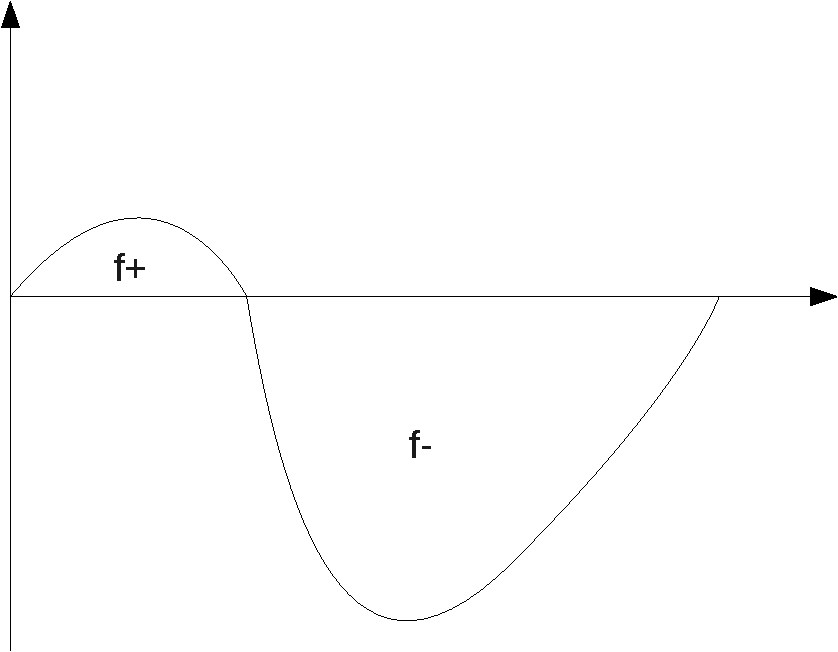
\includegraphics[scale=0.3]{images/fplus_fmoins.pdf}
\caption{Séparation partie positive/partie négative}\label{ch3:fig1}
\end{figure}
Pour toute application mesurable $f$, les applications $f^+,f^-$ sont
mesurables positives et admettent donc une intégrale. La définition de
l'intégrale de $f$ se fera à partir de celles de $f^+,f^-$.
\begin{mandatory}
\begin{defn}
Soit $f$ mesurable. On dira que $f$ est sommable si $f^+, f^-$ sont
sommables et on posera~:
\[
\int_E f d \mu = \int_E f^+ d \mu - \int_E f^- d \mu
\]
\end{defn}
\end{mandatory}
On notera que $|f|=f^++f^-$. Si $f$ est sommable, alors $|f|$ est sommable.
Réciproquement, si $|f|$ est sommable, alors $f^+,f^-$ sont nécessairement
sommables car:
\[
\int_E f^+ d \mu \leq \int_E |f| d \mu \quad \int_E f^- d \mu \leq \int_E |f|
\]
Il est donc équivalent, pour tester la sommabilité de $f$ de vérifier que $f$
est mesurable et que:
\[
\int_E |f| d \mu < +\infty
\]
C'est cette méthode qui est le plus souvent employée en pratique.
\begin{exercice}
Avec les notations et définitions de l'exercice \ref{ch3:ex1}, montrer que les
applications sommables sur $\left(\mathbb{N},\mathcal{P}(\mathbb{N})\right)$
sont les séries absolument convergentes.
\end{exercice}
On peut étendre la notion de sommabilité aux applications à valeurs complexes:
$f\colon E \to \mathbb{C}$ sera dite sommable si $\Re(f), \Im(f)$ sont
des applications sommables et on posera:
\[
\int_E f d\mu = \int_E \Re(f) d \mu + i \int_E
\Im(f) d \mu
\]
Une application mesurable $f \colon \mathbb{R} \to \mathbb{C}$ sera sommable si
et seulement $\Re(f), \Im(f)$ sont des applications mesurables et si:
\[
\int_E |f(x)| d \mu < +\infty
\]

\begin{mandatory}
\begin{prop}
Soient $f,g$ applications sommables et soit $\lambda \in \mathbb{R}$.
$\lambda f + g$ est sommable et~:
\[
\int_E \left( \lambda f + g\right) d \mu = \lambda \int_E f  d \mu + \int_E g d
\mu
\]
Si $f \leq g$~:
\[
\int_E f d \mu \leq \int_E g d \mu
\]
\end{prop}
\end{mandatory}
\begin{proof}
Supposons $\lambda > 0$. $(\lambda f )^+ =\lambda f^+$ et $(\lambda f + g)^+
\leq \lambda f^+ + g ^+$ d'où $(\lambda f + g )^+$ sommable. Un
raisonnement similaire sur les parties négatives montre que $(\lambda
f + g)^-$ est sommable, donc $\lambda f + g$ est
sommable. Par ailleurs, en décomposant $f$ et $g$ en parties positives
et négatives on a~
\[
\lambda f + g = \lambda f^+ + g^+ -(\lambda f^- +
g^-)
\]
d'où l'on obtient~:
\[
\int_E \lambda f + g d \mu = \lambda \int_E f d \mu + \int_E g d\mu
\]
Le cas $\lambda < 0$ se traite similairement en remarquant que
$(\lambda f)^+ = - \lambda f^-$.
Enfin, si $f \leq g$, $g-f \leq0$ est sommable d'intégrale $\int_E g-f
d \mu \geq 0 $, d'où $\int_E g d\mu - \int_E f d \mu \geq 0$.
\end{proof}
\begin{mandatory}
\begin{prop}
Soit $f$ une application sommable. On a~:
\[
\left |  \int_E f d \mu \right | \leq \int_E |f| d \mu
\]
\end{prop}
\end{mandatory}
\begin{proof}
$|f| = f^+ + f^-$ et~:
\[
\left | \int_E \left(f^+ - f^-\right) d \mu \right | \leq \int_E f^+ d \mu +
\int_E f^- d \mu = \int_E |f| d \mu
\]
\end{proof}
Le changement de variable et la relation de Chasles sont inchangées pour les
intégrales d'applications sommables.

\begin{defn}
Soit $(E, \mathcal{T}, \mu)$ un espace mesurable. Soit $\mathcal{P}$
une propriété définie sur $E$. On dira que $\mathcal{P}$ est vraie
$\mu$-presque partout (ou simplement presque partout si aucune
ambiguïté n'est possible sur la mesure) si~:
\[
\mu \left (
\{
x | \mathcal{P}(x) \mbox{ faux }
\}
\right ) = 0
\]
\end{defn}
\begin{mandatory}
\begin{prop}\label{ch2:upp}
Soient $f,g$ deux applications mesurables égales $\mu$-presque
partout. Si $g$ est sommable, alors $f$ est sommable et $\int_E f d
\mu = \int_E g d \mu$. 
\end{prop}
\end{mandatory}
\begin{proof}
Supposons dans un premier temps $f,g$ positives et $g$ sommable. 
Soit l'ensemble $A =
\{ x | f(x) \neq g(x) \}$.
La formule de Chasles donne ~:
\[
\int_E f\wedge n  d \mu = \int_A f\wedge n d \mu + \int_{A^c} f \wedge n d \mu
\]
Sur $A^c$, $f=g$ et donc:
\[
\int_{A^c} f \wedge n d \mu = \int_{A^c} g \wedge n d \mu
\]
D'où, comme $\mu(A)=0$ par hypothèse:
\[
\int_E f\wedge n  d \mu \leq \int_{A^c} g \wedge n d \mu + n \mu(A)\leq
\int_{E} g d \mu
\]
Par un passage à la limite, 
$\int_E f d\mu \leq \int_E g d \mu$, ce qui montre la sommabilité de $f$.
En échangeant les rôles de $f$ et $g$, on obtient finalement: $\int_E f d \mu =
\int_E g d \mu$. Si les applications ne sont pas positives mais sommables, on
applique le résultat précédent aux parties positives et négatives. 
\end{proof}
On utilise le plus souvent l'abbréviation $\mu\text{-pp}$ pour signifier qu'une
propriété est vraie $\mu$ presque partout.

% \chapter{Convergence dominée}
La puissance de la théorie de l'intégration de Lebesgue réside dans
les théorèmes de convergence que l'on peut en déduire. Historiquement,
la première théorie de l'intégration formalisée est celle de Riemann qui a été
présentée en introduction. Son défaut principal est la nécessité d'avoir
 la convergence uniforme pour intervertir limite et intégrale. Dans le cadre de
 la théorie de Lebesgue, la convergence simple suffit, en ajoutant, dans le cas
 d'applications de signe quelconque, une hypothèse aisée à vérifier. Une conséquence
importante des théorèmes qui vont être maintenant établis sera l'existence
d'espaces d'applications sommables qui pourront être munis d'une structure
d'espace de Banach.

\begin{mandatory}
\begin{theorem}\label{ch2:mono} Convergence monotone positive. Soit $(f_n)_{n \in \mathbb{N}}$ une suite croissante d'applications
mesurables positives sur $(E, \mathcal{T}, \mu)$. 
Sa limite simple $f$ existe, est mesurable et
l'on a~:
\[
\int_E f d \mu = \lim_{n \to +\infty} \int_E f_n d \mu
\]
\end{theorem}
\end{mandatory}
\begin{proof}
L'existence de $f$ ne pose aucun problème, la suite $(f_n)$ étant
supposée croissante (il est possible que $f$ prenne la valeur
$+\infty$ sur une partie de $E$). La mesurabilité de $f$ découle de la
mesurabilité d'une limite simple d'applications mesurables. 
Pour tout entier $n$, soit $(\phi_{n,k})_{k \in \mathbb{N}}$ une
suite croissante d'applications étagées convergeant simplement vers
$f_n$ (une telle suite existe en vertu de la proposition
\ref{ch2:1}). On pose pour tout entier $n \in \mathbb{N}, g_n =
sup_{k=0 \dots n} \phi_{k,n}$. $g_n$ est étagée et la suite $(g_n)$
est croissante. Par ailleurs, pour tout entier $k$, on vérifie
aisement que~:
\[
f_k \leq \lim_n g_n \leq f
\]
d'où, en faisant tendre $k$ vers $+\infty$, $\lim_n g_n = f$. Par la
proposition \ref{ch2:2}, on obtient~:
\[
\int_E f d \mu =  \lim_n \int_E g_n d \mu
\]
Par définition de $g_n$, $\int_E g_n d \mu \leq \int_E f_n d \mu$, d'où~:
\[
\int_E f d \mu = \lim_n \int_E g_n d \mu \leq \lim_n \int_E f_n d \mu
\]
comme l'inégalité $\int_E f d \mu \geq \int_E f_n d \mu$ est évidente,
on en déduit l'égalité.
\end{proof}
\begin{rem}
L'argument diagonal utilisé dans cette démonstration est un grand classique des
mathématiques: il faut le connaître et savoir l'utiliser!
\end{rem}
\begin{mandatory}
\begin{theorem}\label{ch2:beppo} Beppo-Levi.
Soit $(f_n)_{n \in \mathbb{N}}$ une suite croissante d'applications
sommables telle qu'il existe $M >0$ avec~:
\[
\forall n \in \mathbb{N}, \, \int_E |f_n|d \mu \leq M
\] 
alors $(f_n)$ converge presque partout vers une application sommable
$f$ et~:
\[
\lim_n \int_E f_n d \mu = \int_E f d\mu
\]
\end{theorem}
\end{mandatory}
\begin{proof}
On remarque tout d'abord que la suite $(f_n)$ étant croissante, elle
admet une limite simple $f$ (pouvant éventuellement être infinie sur
une partie de $E$).
Pour tout $n$, l'application $g_n = f_n -f_0$ est positive sommable car~:
\[
\int_E |f_n - f_0| d \mu \leq 2 M
\]
Le théorème \ref{ch2:mono} s'applique à la suite $(g_n)$ d'où~:
\[
\lim_n \int_E g_n d \mu = \int_E f - f_0 d \mu
\]
d'où~:
\[
\lim_n \int_E f_n d \mu = \int_E f d \mu
\]
Mais par ailleurs $\forall n \in \mathbb{N}, \int_E |f_n| d \mu \leq
M$ et donc $\int_E |f| d \mu$ est finie. On en déduit alors que la
partie de $E$ sur laquelle $f$ n'est pas finie est de mesure nulle, ce
qui termine la preuve.
\end{proof}
\begin{mandatory}
\begin{theorem}\label{ch2:fatou} Lemme de Fatou.
Soit $(f_n)_{n \in \mathbb{N}}$ une suite d'applications mesurables non
  négatives. On a~:
\[
\int_E (\liminf_n f_n) d \mu \leq \liminf_n \left(\int_E f_n d \mu \right)
\]
\end{theorem}
\end{mandatory}
\begin{proof}
Pour tout entier $n$, soit $g_n = \inf_{k \geq n} f_k$. On a~:
\[
\liminf_n f_n = \lim_n g_n
\]
La suite $(g_n)$ vérifie les hypothèse du théorème \ref{ch2:mono}, on
a donc~:
\[
\int_E \liminf_n f_n d\mu = \lim_n \int_E g_n d\mu \leq \liminf_n
\int_E f_n d \mu
\]
\end{proof}
\begin{mandatory}
\begin{theorem}\label{ch2:domi} Convergence dominée.
Soit $(f_n)$ une suite d'applications mesurables convergeant
 simplement $\mu$-presque partout vers une application
$f$ et telles qu'il existe
une application sommable $g$ avec~:
\[
\forall n \in \mathbb{N}, \, |f_n| \leq g \quad \mu\text{-pp}
\]
Alors~:
\begin{itemize}
\item $f$ est sommable.
\item $\lim_n \int_E f_n d\mu  = \int_E f d\mu$.
\item $\lim_n \int_E |f_n -f | d \mu = 0$.
\end{itemize}
\end{theorem}
\end{mandatory}
\begin{proof}
On peut supposer que la convergence simple a lieu partout, le
comportement sur un ensemble de mesure nulle ne modifiant en rien les
intégrales. 
Les applications $f_n$ sont sommables car~:
 \[\int_E |f_n| d \mu \leq
\int_E g d \mu < +\infty \]
Par passage à la limite, $|f| \leq g$ d'où la sommabilité de $f$.
En remarquant que pour tout $n$, $|f_n - f| \leq 2g$, le lemme de
Fatou permet d'écrire~:
\[
\liminf_n \int_E (2g -|f_n-f|) d \mu \geq \int_E \liminf_n (2g - |f_n-f|)
d \mu
\]
par hypothèse, $f_n \to f$ d'où~:
\[
 \liminf_n \left (2g - |f_n-f| \right ) = 2g
\]
La linéarité de l'intégrale donne alors~:
\[
\liminf_n \int_E (2g -|f_n-f|) d \mu = 2 \int_E g d \mu - \limsup_n
\int_E |f_n-f| d \mu = 2 \int_E g d \mu
\]
soit~:
\[
 \limsup_n \int_E |f_n-f| d \mu = 0
\]
ce qui prouve le point 3) du théorème.
Comme~:
\[
\left | \int_E f_n d \mu - \int_E f d \mu \right | \leq \int_E |f_n
-f| d \mu
\]
le point 2) en découle immédiatement.
\end{proof}
\begin{rem}
\begin{itemize}
\item Les conclusions du théorème de convergence dominée (ainsi que des
précédents) s'appliquent si l'on remplace les suites d'applications
par des familles $(f_\lambda)_{\lambda \in I}$ avec $I$ un ensemble
d'indice muni d'une structure d'espace métrique. 
\item Il est très important de prendre garde au fait que l'application
  $g$ ne peut en aucun cas dépendre de $n$~: c'est une source
  fréquente d'erreurs.
\end{itemize}
\end{rem}
Il convient de toujours bien vérifier l'hypothèse de domination, qui peut se
révéler délicate, comme l'exercice suivant va le montrer.
\begin{exercice}
\begin{itemize}
\item Soit la suite d'applications $(f_n)$ définies sur $[0,1]$ par~:
\[
\forall x \in [0,1], \, f_n(x) = \frac{nx}{1+n^2x^2}
\]
Déterminer la limite simple de cette suite. Conclure quant à la limite de~:
\[
\int_{[0,1]} f_n(x) d \lambda(x)
\]
\item On considère maintenant la suite $(g_n)$, applications définies sur $\mathbb{R}$ par~:
\[
g_n(x) = \frac{1}{n} 1_{[0, n]}
\]
Déterminer la limite simple de cette suite. Peut-on appliquer le théorème de convergence
dominée à~:
\[
\int_{\mathbb{R}} g_n(x) d\lambda(x)
\]
\end{itemize}
\end{exercice}
\section{Applications}
\subsection{Intégrales dépendant d'un paramètre}
\begin{prop}\label{ch2:contpar} Continuité des intégrales dépendant
  d'un paramètre.
Soit $(M,d)$ un espace métrique, $\lambda_0 \in M$, $(E, \mathcal{T},\mu)$ un espace mesuré et soit $F : M \times E \to
\mathbb{R}$ une application telle que~:
\begin{itemize}
\item Pour tout $\lambda \in M$, l'application $x \to f(\lambda,x)$
  est mesurable.
\item L'application $\lambda \to f(\lambda,x)$ est continue en
  $\lambda_0$ pour $\mu$-presque tout $x$.
\item Il existe une application sommable $g$ et un voisinage $V$ de
  $\lambda_0$ tels que~:
\[
\forall \lambda \in V, \, |F(\lambda,x)| \leq g(x)
\]
pour $\mu$-presque tout $x$.
alors l'application~:
\[
\lambda \in V \to \int_E F(\lambda,x) d\mu(x)
\]
est bien définie et est continue en $\lambda_0$.
\end{itemize}
\end{prop}
\begin{proof}
La sommabilité de l'application $x \to F(\lambda,x)$ est acquise pour
$\lambda \in V$ par l'hypothèse de domination. Par ailleurs, soit
$(\lambda_n)$ une suite de points de $V$ de limite $\lambda_0$. Le
théorème de convergence dominée donne~:
\[
\lim_n \int_E F(\lambda_n,x)d\mu(x) = \int_E \lim_n  F(\lambda_n,x)d\mu(x) =
\int_E F(\lambda_0,x)d\mu(x)
\]
ce qui prouve la continuité en $\lambda_0$ de l'intégrale dépendant du
paramètre $\lambda$.
\end{proof}
\begin{prop}\label{ch2:derpar} Dérivabilité des intégrales dépendant
  d'un paramètre.
Soit $I$ un intervalle ouvert de $\mathbb{R}$, $y_0 \in I$, et soit $F : I \times E \to
\mathbb{R}$ une application telle que~:
\begin{itemize}
\item Pour tout $y \in I$, l'application $x \to F(y,x)$ est sommable.
\item L'application $y \to F(y,x)$ est dérivable en $y_0$ pour $\mu$-presque
  tout $x$. On notera~:
\[
\frac{\partial F}{\partial y}
\]
l'application égale à la dérivée de $F$ par rapport à $y$ en tout
point $x$ où elle est définie et prenant une valeur arbitraire
ailleurs.
\item Il existe une application sommable $g$ telle que pour tout $y
  \in I$~:
\[
|F(y,x)-F(y_0,x)| \leq g(x) |y-y_0|
\]
pour $\mu$-presque toute valeur de $x$.
\end{itemize}
Alors l'application~:
\[
\lambda \to \int_E F(y,x)d\mu(x)
\]
est dérivable en $y_0$ et sa dérivée vaut~:
\[
 \int_E \frac{\partial F(y_0,x)}{\partial y} d \mu(x)
\]
\end{prop}
\begin{proof}
La démonstration est une application immédiate du théorème de
convergence dominée à la suite~:
\[
\frac{F(y_n,x)-F(y_0,x)}{y_n -y_0}
\]
avec $y_n \to y_0$.
\end{proof}
\begin{rem}
Le théorème des accroissement finis montre que si il existe $g$
sommable telle que~:
\[
\forall y \in I, \, \left |
\frac{\partial F(y,x)}{\partial y} 
\right | \leq g(x)
\]
pour $\mu$-presque tout $x$, alors l'hypothèse 3) de la proposition
est automatiquement vérifiée. 
\end{rem}
\subsection{Sommabilité terme à terme}
Soit $(f_n)_{n \in \mathbb{N}}$ une suite d'applications mesurables
telle que~:
\[
\sum_{n \in \mathbb{N}} \int_E |f_n| d \mu < +\infty
\]
alors~:
\begin{itemize}
\item $\sum_{n \in \mathbb{N}} f_n$ converge absolument $\mu$-presque
  partout et est som\-mable.
\item On a~:
\[
\sum_{n \in \mathbb{N}} \int_E f_n d \mu = \int_E \sum_{n \in
  \mathbb{N}} f_n d \mu 
\]
\end{itemize}
\begin{proof}
Soit $g_n = \sum_{k = 0 \dots n} |f_n|$. La suite $g_n$ est
positive croissante, le théorème de convergence monotone s'applique
et~:
\[
\lim_n \int_E g_n d \mu = \int_E \lim_n g_n d \mu 
\]
Or par hypothèse~:
\[
\lim_n \int_E g_n d \mu = \sum_n \int_E |f_n| d \mu < +\infty
\]
la limite $g$ de la suite $g_n$ est sommable, donc $g$ est finie
$\mu$-presque partout. On en déduit la convergence absolue
$\mu$-presque partout de la serie de terme général $f_n$.
Par ailleurs, le théorème de convergence dominée s'applique aux sommes
partielles de la série de terme général $f_n$ en prenant comme application
dominante~:
\[
\sum_n |f_n|
\]
Ceci montre la seconde partie de la proposition.
\end{proof}
\begin{exercice}
Soit $f : \mathbb{R} \to \mathbb{R}$ une application sommable. On 
définit l'application $\phi : \mathbb{R} \to \mathbb{C}$ par~:
\[
\forall \xi \in \mathbb{R}, \, \phi(\xi) = \int_{\mathbb{R}} f(t) e^{-i 2 \pi \xi t} d \lambda(t)
\]
\begin{itemize}
\item Montrer que $\phi$ est bien définie et est continue sur $\mathbb{R}$.
\item On suppose maintenant que $f$ est telle que~:
\[
\int_{\mathbb{R}} | t f(t) | d \lambda(t) < +\infty
\]
Montrer que $\phi$ est dérivable et calculer sa dérivée.
\end{itemize}
\end{exercice}
On peut dans certains cas utiliser le théorème de convergence dominée pour
calculer la valeur d'intégrales généralisées (qui ne sont pas des intégrales au
sens strict, mais uniquement des limites). Un cas classique est la détermination
de l'intégrale de $\sin x / x$ sur $\mathbb{R}$, qui est un exercice
fréquemment traité en classes préparatoires.
\begin{exercice}
Soit l'application $f : \mathbb{R} \to \mathbb{R}$~:
\[
x \to \left \{
\begin{array}{cc}
\frac{\sin x}{x} & x > 0 \\
1 & x = 0 \\
0 & x < 0
\end{array}
\right .
\]
\begin{itemize}
\item Montrer que $f \notin L^1, f \in L^2$.
\item Montrer que pour tout réel $a > 0$ l'application~:
\[
F : a \to \int_{\mathbb{R}} f(x) e^{-ax} dx
\]
est bien définie et est dérivable sur $\mathbb{R}^{+*}$.
\item Calculer $lim_{a \to +\infty} F(a)$ et en déduire une expression simple de $F$.
\item Montrer que $F$ se prolonge par continuité à droite en 0 et calculer $F(O^+)$.
\end{itemize}
La valeur obtenue pour $F(0^+)$ est aussi celle de l'intégrale généralisée de
$\sin x/ x$ sur $\mathbb{R}^+$.
\end{exercice}
\subsection{Intégrale de Riemann}
L'intégrale au sens de Riemann d'une application bornée sur un compact est,
lorsqu'elle existe, de m\^eme valeur que celle de Lebesgue qui  existe
nécessairement elle aussi. La suite de cette section va établir ce résultat.
 Dans cette partie, $f : [a,b] \to \mathbb{R}$ est une
application \textit{bornée}.
\begin{defn}
Une subdivision $\mathcal{P}$ de l'intervalle $[a,]$ est une suite de
réels $(x_i)_{i=0}^{N}$ telle que $a=x_0 < x_1 < \dots < x_{N-1} < x_N
= b$. Le pas d'une subdivision est~:
\[
\inf_{n=0\dots N-1} (x_{n+1} -x_n)
\]
Enfin, on dira qu'une subdivision $\mathcal{P}_1$ est plus fine qu'une
subdivision $\mathcal{P}_2$ si tout point de $\mathcal{P}_2$
appartient aussi à $\mathcal{P}_1$.
\end{defn}
\begin{defn}
Une application en escalier sur $[a,b]$ est une application de la
forme~:
\[
\sum_{n=0}^{N-1} y_n 1_{[x_n, x_{n+1}[}
\]
avec $(y_n)_{n=0\dots N-1}$ réels et $(x_n)$ subdivision de $[a,b]$.
\end{defn}
\begin{defn}
Soit $f= \sum_{n=0}^{N-1} y_n 1_{[x_n, x_{n+1}[}$ une application en
    escalier. L'intégrale de Riemann de $f$ est la quantité~:
\[
\int_a^b f(x) dx = \sum_{n=0}^{N-1} y_n (x_{n+1} -x_n)
\]
\end{defn}
\begin{defn}
Soit $f$ bornée sur $[a,b]$. L'intégrale inférieure (resp. supérieure)
de $f$ est~:
\[
\sup \left \{ \int_a^b h(x) dx, h \mbox{ en escalier }, h \leq f \right
\}
\]
resp.
\[
\inf \left \{ \int_a^b h(x) dx, h \mbox{ en escalier }, h \geq f \right
\}
\]
Si les deux quantités sont égales, on dit que $f$ est
Riemann-intégrable et l'intégrale de $f$, notée $\int_a^b f(x) dx$ est
la valeur commune.
\end{defn}
\begin{theorem}
Une application $f$ bornée sur $[a,b]$ est Riemann-intégrable si et
seulement si elle est égale presque partout (relativement à la mesure
de Lebesgue) à une application continue. On a en outre~:
\[
\int_a^b f(x) dx = \int_{[a,b]} f d \lambda
\]
avec $\lambda$ mesure de Lebesgue.
\end{theorem}
\begin{proof}
Il est facile de remarquer que toute application en escalier étant une
application étagée, les deux intégrales coïncident pour cette classe
d'applications. 
Supposons tout d'abord $f$ Riemann-intégrable.
Soit $(h_n)_{n \in \mathbb{N}}$ une suite d'applications en escaliers
 telle que $\forall n, h_n \geq f$ et
$\lim_n \int_a^b h_n(x) dx = \int_a^b f(x) dx$. On peut, sans perte de
généralité, supposer la suite $h_n$ décroissante.  Elle converge
vers une limite $h$ et par application du thèorème de convergence
dominée (on peut majorer $|h_n|$ par une constante qui est sommable
sur le compact $[a,b]$)~: 
\[
\int_{[a,b]} h d \lambda = \lim_n \int_{[a,b]} h_n d \lambda = \lim_n \int_a^b
h_n(x) dx = \int_a^b f(x) dx
\]
De même, on peut choisir une suite croissante d'applications en
escalier $(g_n)$, telle que $g_n \leq f$ pour tout $n$ et $\lim_n
\int_a^b g_n(x) dx = \int_a^b f(x) dx$. Le théorème de convergence
dominée s'applique à nouveau et l'on a~:
\[
\int_{[a,b]} g d \lambda = \int_a^b f(x) dx
\]
avec $g$ limite de la suite $(g_n)$. 
On en déduit~:
\[
\int_{[a,b]} (h-g) d \lambda = 0
\]
Soit $h(x)=g(x)=f(x)$ pour $\lambda$-presque toute valeur de
$x$. Comme $h$ et $g$ sont des limites de fonctions en escalier, elles
ne peuvent présenter qu'un ensemble dénombrable de points de
discontinuité, d'où $f$ est égale  $\lambda$-presque partout à une
application continue et l'intégrale de Riemann coïncide avec celle de Lebesgue.
Supposons maintenant que l'on se donne $f$ bornée, égale
$\lambda$-presque partout à une application continue. Soit
$\mathcal{P}_n$ la partition de $[a,b]$ qui comporte $2^n + 1$ points
$x_{i,n}, i=0 \dots 2^n$ divisant $[a,b]$ en segments égaux. Soit
$M_{i,n}$ le maximum (resp. $m_{i,n}$ le minimum) de$f$ sur
chaque intervalle $[x_{i,n}, x_{i+1,n}]$. On pose $g_n =
\sum_{i=0}^{2^n-1} m_{i,n} 1_{[x_{i,n}, x_{i+1,n}[}$,
    $h_n=\sum_{i=0}^{2^n-1} M_{i,n} 1_{[x_{i,n}, x_{i+1,n}[}$.
	$f$ étant égale presque partout à une application continue, les suites
	$(g_n),(h_n)$ convergent $\lambda$-presque partout vers $f$ et
	par application du théorème de convergence dominée~:
\begin{align*}
\int_{[a,b]} f d \lambda = & \lim_n \int_{[a,b]} g_n d\lambda = \lim_n
\int_a^b g_n(x) dx \\  
= & \lim_n \int_{[a,b]} h_n d\lambda = \lim_n \int_a^b h_n(x) dx
\end{align*}
L'application $f$ est donc Riemann-intégrable et les deux intégrales
sont égales.
\end{proof} 
Ce résultat montre que, sur un compact, on peut se permettre d'utiliser
l'une ou l'autre intégrale dès lors que l'application est égale
presque partout à une application continue. Ceci induit à confondre
par abus de notation $\int_a^b$ avec $\int_{[a,b]}$.
Toute application $f$ qui est limite uniforme d'applications en escalier admet
une primitive $F$. On peut utiliser le résultat précédent pour calculer dans ce
cas l'intégrale de Lebesgue sur un compact $[a,b]$ à l'aide de $F$:
\[
\int_{[a,b]}f(t) d \lambda(t) = F(b) - F(a)
\]

\begin{rem}
Il convient d'être d'une extrême prudence avec ce que l'on appelle les
intégrales généralisées !
Dans le cas d'intervalles infinis (semi-infinis) ou d'ouverts, la
notation~:
\[
\int_a^b f(x) dx
\]
désigne, si elle existe, la limite~:
\[
\lim_{x\to a^+, y \to b^-} \int_x^y f(x) dx
\]
Il ne s'agit donc pas, à proprement parler, d'une intégrale de
Riemann. Dans le cadre de la théorie de Lebesgue, il n'y a pas de
problème de définition même si l'on n'intègre pas sur un compact, et la
notion d'intégrale généralisée n'a pas de sens. Dans ce cas, il
convient donc de bien distinguer les notations. Cependant, si une
application $f$ est telle que $\int_a^b |f(x)|dx$ existe (on dit alors
que $f$ admet une intégrale généralisée absolument convergente),
l'intégrale de Lebesgue de $f$ existe sur le même domaine et avec la
même valeur (application immédiate du théorème de convergence dominée).
\end{rem}
% \chapter{Intégrales multiples}
\section{tribu produit}
\begin{mandatory}
\begin{defn}
Soient deux espaces mesurables $(E, \mathcal{T})$,$(F, \mathcal{F})$. La tribu
produit sur $E\times F$ est la plus petite tribu rendant les projections
canoniques $\pi_E,\pi_F$ mesurables. On la note $\mathcal{T}\otimes
\mathcal{F}$.
\end{defn}
\end{mandatory}
Il est possible de caractériser de façon simple cette tribu: pour que la
projection $\pi_E$ (resp. $\pi_F$) soit mesurable, il faut que pour tout $A \in
\mathcal{T}$ (resp. $B \in \mathcal{F}$) l'image réciproque $\pi^{-1}(A) = A
\times F$ (resp. $\pi_F^{-1}(B) = E \times B$) soit dans $\mathcal{T}\otimes \mathcal{F}$.
Par intersection entre ensembles de la forme précédente, on en déduit que tous
les produits cartésiens $A \times B$ avec $A \in
\mathcal{T}$, $B \in \mathcal{F}$ sont dans $\mathcal{T}\otimes \mathcal{F}$.
Cette tribu contient donc la tribu engendrée par ces produits cartésiens.
Réciproquement, la tribu engendrée par les produits cartésiens contient les
ensembles de la forme $A \times F$, $E \times B$, donc rend les projections
canoniques mesurables et contient ainsi $\mathcal{T}\otimes \mathcal{F}$: les
deux tribus sont donc égales.
\begin{defn}
Soient $E,F$ deux ensembles. Soit $A \subset E \times F$. Soit $x \in
E$ (resp $y \in F$) La section de $A$ selon $x$
(resp. $y$) est l'ensemble $A_x \subset F$ (resp $A^y \subset E$) defini par~:
\[
A_x = \{ v \in F | (x,v) \in A \}
\]
resp.
\[
A^y = \{ u \in E | (u,y) \in A \}
\]
\end{defn}
Pour une application $f$ définie sur $E \times F$, on construira de même
les sections~:
\[
f_x : v \in F  \to f(x,v) \, \quad f^y : u \in E \to f(u,y)
\]
\begin{prop}
Soit $(E, \mathcal{T}), (F, \mathcal{F})$ deux espaces mesurables avec
$\mu,\nu$ mesures $\sigma$-finies. 
\begin{itemize}
\item Si $A \subset E \times F$ appartient à la tribu produit
$\mathcal{T} \otimes \mathcal{F}$ alors les sections $A_x,A^y$ sont
respectivement $\mathcal{F}$ et $\mathcal{T}$ mesurables pour toute
valeur de $x$ et $y$.
\item Si $f$ est une application définie sur $E \times F$ et
mesurable, alors ses sections sont mesurables.
\end{itemize}
\end{prop}
\begin{proof}
La preuve utilise un classique argument de minimalité. Soit $x  \in E$
et soit $\mathcal{G} = \{ A \in \mathcal{T} \times \mathcal{F} | A_x
\in \mathcal{F} \}$. On a~:
\begin{itemize}
\item $\emptyset \in \mathcal{G}$.
\item $E \times F \in \mathcal {G}$.
\end{itemize}
de plus, $(A_x)^c = A^c_x$ d'où la stabilité de $\mathcal{G}$ par
passage au complémentaire. Enfin, pour toute famille dénombrable
$(A_n)$ d'éléments de $\mathcal{G}$, $(\cup_n A_n)_x = \cup_n
(A_n)_x$. L'ensemble $\mathcal{G}$ est donc une tribu. Elle contient
tous les rectangles $A \times B$ avec $A\in \mathcal{T}, B \in
\mathcal{F}$. Par minimalité de la tribu produit, elle contient donc
$\mathcal{T} \otimes \mathcal{F}$. 
La proposition relative aux sections d'applications en découle immédiatement.
\end{proof}
\section{Théorème de Fubini}

\begin{prop}
Soient $(E, \mathcal{T}, \mu), (F, \mathcal{F}, \nu)$ deux espaces
mesurés avec $\mu,\nu$ mesures $\sigma$-finies. 
Si $A \in \mathcal{T} \times \mathcal{F}$, l'application $x
\to \nu(A_x)$ (resp. $y \to \mu(A^y)$) est mesurable.
\end{prop}
\begin{proof}
Supposons tout d'abord que la mesure $\nu$ soit finie. Soit
$\mathcal{G} = \{ A \in \mathcal{T} \times \mathcal{F} | x \to
\nu(A_x) \mbox { mesurable } \}$. Tous les rectangles de la forme  $A
\times B$ avec $A\in \mathcal{T}, B \in \mathcal{F}$ sont dans
$\mathcal{G}$ car $\nu((A \times B)_x) = \nu(B) 1_A(x)$. Soient $A,B
\in \mathcal{G}$ avec $A \subset B$. On a $\nu((B-A)_x) = \nu(B_x) -
\nu(A_x)$ donc $A - B \in \mathcal{G}$. Si $(A_n)$ est une famille
dénombrable croissante d'éléments de $\mathcal{G}$, comme~:
\[
\nu((\cup_n(A_n))_x) = \nu(\cup_n (A_n)_x) = \lim_n \nu((A_n)_x)
\]
on a $\cup_n A_n \in \mathcal{G}$. L'ensemble $\mathcal{G}$ est une
classe monotone. On vérifie qu'elle est stable par intersections
finies, ce qui montre qu'elle est égale à la tribu $\mathcal{T} \times
\mathcal{G}$ d'où la proposition. 
Si la mesure est $\sigma$-finie, on étend le résultat obtenu en
prenant un recouvrement dénombrable par des ensembles de $\nu$-mesure finie.
\end{proof}
\begin{mandatory}
\begin{theorem}
Sous les hypothèses de la proposition précédente, il existe une unique
mesure sur $\mathcal{T} \otimes \mathcal{F}$, notée $\mu \otimes \nu$,
telle que $\mu\otimes \nu (A \times B) = \mu(A) \nu(B)$ pour $A \in
\mathcal{T}, B \in \mathcal{F}$. De plus, on a~:
\[
\forall A \in \mathcal{T} \otimes \mathcal{F} \, , \mu \otimes \nu (A) = \int_E
\nu(A_x) d \mu = \int_F \mu(A^y) d \nu
\]
\end{theorem}
\end{mandatory}
\begin{proof}
La démonstration est élémentaire dès lors que la proposition
précédente est prouvée et est laissée à titre d'exercice.
\end{proof}
Dans le cas où $\mu$ et $\nu$ sont égales à la mesure de Lebesgue sur
$\mathbb{R}$, la mesure produit est la mesure de Lebesgue sur $\mathbb{R}^2$ qui
à un produit cartésien d'intervalles associe sa surface. On peut étendre sans
difficulté ce résultat à $\mathbb{R}^n$.
\begin{mandatory}
\begin{theorem}(Tonnelli)
Soient $(E, \mathcal{T}, \mu), (F, \mathcal{F}, \nu)$ deux espaces
mesurés avec $\mu, \nu$ mesures $\sigma$-finies et soit $f : E \times F \to \mathbb{R}^+$ une application
mesurable. 
\begin{itemize}
\item L'application $x \to  \int_F f_x d \nu $ (resp. $y \to
\int_E f^y d \mu$) est mesurable.
\item On a:
 \begin{align*}
\int_{E \times F} f d( \mu \otimes \nu) & = \int_E \left (
\int_F f_x d \nu \right ) d \mu \\
& = \int_F \left (
\int_E f^y d \mu \right ) d \nu
\end{align*}
\end{itemize}
\end{theorem}
\end{mandatory}
\begin{proof}
Le théorème est immédiat si $f = 1_A$ avec $A \in \mathcal{T} \times
\mathcal{F}$. Par linéarité de l'intégrale, il reste vrai sur les
applications étagées positives, puis, par convergence monotone sur
toutes les applications mesurables positives.
\end{proof}
Comme dans pratiquement tous les cas en théorie de Lebesgue, il faut traiter
séparément le cas des applications de signe quelconque, en adjoignant
l'hypothèse de sommabilité. Le théorème suivant est souvent appliqué en ayant au
préalable utilisé le théorème de Tonnelli sur la valeur absolue de l'application
à intégrer.
\begin{mandatory}
\begin{theorem}(Fubini)
Soient $(E, \mathcal{T}, \mu), (F, \mathcal{F}, \nu)$ deux espaces
mesurés et avec $\mu,\nu$ mesures $\sigma$-finies. Soit $f : E \times F \to
\mathbb{R}$ une application sommable par rapport à $\mu \otimes \nu$.
\begin{itemize}
\item Pour $\mu$-presque tout $x\in E $ (resp. $\nu$-presque tout $y
\in  F$), l'application $f_x$ (resp. $f^y$) est sommable.
\item En posant~:
\[
I : x \to \left \{
\begin{array}{cc}
\int_F f_x d \nu & \mbox { si } f_x \mbox { sommable } \\
0 & \mbox{ sinon }
\end{array}
\right .
\]
\[
J : y \to \left \{
\begin{array}{cc}
\int_E f^y d \mu & \mbox { si } f^y \mbox { sommable } \\
0 & \mbox{ sinon }
\end{array}
\right .
\]
on a~:
\[
\int_{E \times F} f d (\mu \otimes \nu) = \int_E I(x) d \mu(x) = \int_F J(y)
d \nu(y)
\]
\end{itemize}
\end{theorem}
\end{mandatory}
\begin{proof}
Soit $f^+$ (resp. $f^-$) la partie positive (resp. négative) de
$f$. Les sections $f^+_x$ et $f^-_x$ sont mesurables et par le
théorème de Tonnelli les applications~:
\[
x \to \int_F f^+_x d \nu \, , x \to  \int_F f^-_x d \nu
\]
sont sommables. On en déduit qu'elles sont finies $\mu$-presque partout
et donc que $I$ est $\mu$-sommable. 
Le théorème est obtenu en écrivant~:
\begin{align*}
\int_{E \times F} f d (\mu \otimes \nu) & = \int_{E \times F} f^+ d( \mu
\otimes \nu) - \int_{E \times F} f^- d (\mu \otimes \nu) \\
& = \int_E \left ( \int_F F^+_x d\nu \right ) d \mu -  \int_E \left (
\int_F F^-_x d\nu \right ) d \mu \\
& = \int_E I d \mu 
\end{align*}
\end{proof}
\begin{rem}
L'hypothèse de $\mu \otimes \nu$ sommabilité est fondamentale dans le
théorème de Fubini. Comme mentionné plus haut, on applique le plus souvent le
théorème de Tonnelli à $|f|$ pour pouvoir la montrer.
\end{rem}
Il est d'usage courant de simplifier l'écriture $d(\mu \otimes \nu)$ par $d\mu
d\nu$ en précisant éventuellement les variables d'intégration en argument de
$d\mu$ et $d\nu$. Il ne faut pas oublier néanmoins qu'il s'agit bien de la mesure produit.
\begin{exercice}
Soit la partie $D=[-1,+1]^2$ de $\mathbb{R}^2$. Calculer les intégrales~:
\[
\int_{D} (x^2 +y^2) d \lambda d\lambda \quad, \quad  \int_{D} y e^{xy} d
\lambda d \lambda
\]
\end{exercice}
\begin{exercice}
On dit qu'une application $f : \mathbb{R} \to \mathbb{R}$ est
localement intégrable si elle est sommable sur tout compact de
$\mathbb{R}$. Soient $f,g$ localement intégrables. On pose~:
\[
F : x \to \int_0^x f(t) d \lambda(t) , \quad G : x \to \int_0^x g(t) d
\lambda(t)
\]
\begin{itemize}
\item Montrer, en utilisant l'application~:
\[
h : (x,y) \to 1_{x \leq y} g(x) f(y)
\]
que pour tout intervalle borné $[a,b]$~:
\[
\int_{[a,b]} f(t)(G(t) - G(a)) d\lambda(t) =
\int_{[a,b]}g(t)(F(b)-F(t)) d\lambda(t)
\]
\item En déduire la formule d'intégration par parties~:
\[
\int_{[a,b]} F(t) g(t) d \lambda(t) = F(b)G(b)-F(a)G(a) - \int_{[a,b]}
f(t) G(t) d \lambda(t)
\]
\end{itemize}
\end{exercice}

Attention à l'hypothèse de sommabilité dans Fubini, m\^eme si tout semble
marcher:
\begin{exercice}
On se place sur le même domaine $D$ qu'à l'exercice 12. Soit~:
\[
f : (x,y) \to \frac{xy}{(x^2+y^2)^2}
\]
\begin{itemize}
\item Calculer~:
\[
\int_{[-1,+1]} \left ( \int_{[-1,+1]} f(x,y) d \lambda(x) \right )
d \lambda(y)
\]
et
\[
\int_{[-1,+1]} \left ( \int_{[-1,+1]} f(x,y) d \lambda(y) \right )
d \lambda(x)
\]
\item Peut-on en déduire, par le théorème de Fubini, la valeur de~:
\[
\int_D f(x,y) d \lambda d \lambda
\]
\end{itemize}
\end{exercice}

\section{Changement de variable}

La formule du changement de variable par les $C^1$-difféomorphismes 
dans $\mathbb{R}^n$ est d'une grande importance tant pratique que
théorique. 
Elle est essentiellement basée sur un calcul de
changement de volume pour des cubes élémentaires, puis l'utilisation
du théorème des classes monotones pour passer à des boréliens
quelconques.
Dans la suite on supposera toujours que l'on travaille dans
$\mathbb{R}^n$ muni de sa topologie usuelle.
La première proposition qui va être montrée maintenant est essentiellement une
traduction en terme de mesure image de la propriété géométrique bien connue
selon laquelle le volume d'un parallélépipède de $\mathbb{R}^n$ qui s'appuie sur
les $n$ vecteurs $v_1,\dots v_n$ est donné par $|\det(v_1,\dots,v_n)|$.
\begin{mandatory}
\begin{prop}
Soit $f \colon \mathbb{R}^n \to \mathbb{R}^n$ une application linéaire
inversible de matrice représentative $M$. Pour tout borélien $B$, on
a~:
\[ 
\lambda(f(B)) = |\det(M)| \lambda(B)
\]
\end{prop}
\end{mandatory}
On remarquera que l'application $B \to \lambda(f(B))$ est la mesure
image de $\lambda$ par $f^{-1}$.
\begin{proof}
Soit $B$ un borélien. Pour tout $x \in \mathbb{R}^n$, on a~:
\[
\lambda(f(B + x)) = \lambda(f(B) + f(x)) = \lambda(f(x))
\]
On en déduit que la mesure image de $\lambda$ par $f^{-1}$ est
invariante par translation, donc égale, à une constante multiplicative
près, à la mesure de Lebesgue~:
\[
\exists C >0 \, | \, \forall B \in \mathcal{B}(\mathbb{R}^n), \, \lambda(f(B)) =
C \lambda(B)
\]
Supposons dans un premier temps $M$ orthogonale. La boule unité est
laissée invariante par $f$, d'où $C = 1 = |\det(M)|$ dans ce cas. Supposons
maintenant que $M$ est diagonale, à coefficients diagonaux $\sigma_i,
i=1\dots n$ positifs. L'image de $[0,1]^n$ est $\prod_{i=1\dots n}
[0, \sigma_i]$, d'où l'on déduit $C = \prod_{i=1\dots n} \sigma_i =
|\det(M)|$. Dans le cas général, on applique les deux résultats
précédents à la décomposition en valeurs singulières $M = U \Sigma
V^t$ de $M$, où les deux matrices $U,V$ sont orthogonales et la matrice $\Sigma$
est diagonale.
\end{proof}
\begin{defn}
Une application inversible $f : \mathbb{R}^n \to \mathbb{R}^n$ est
appelée $C^k$-difféomorphisme si elle est de classe $C^k$ ainsi que
son inverse.
\end{defn}
\begin{term}
Soit $f$ une application différentiable . L'application
jacobienne (ou Jacobien) est l'application $J_f : x \to det(f^\prime(x))$. 
\end{term}
Lorsque une application est de classe $C^1$, elle est bien approchée par son
application dérivée au voisinage d'un point quelconque: on peut donc espérer
que la mesure image associée à $f$ ne soit pas très différente de celle
correspondant à l'approximation linéaire de $f$ en chaque point. Cette
situation est résumée en figure \ref{ch3:2}.  
\begin{figure}[h]
 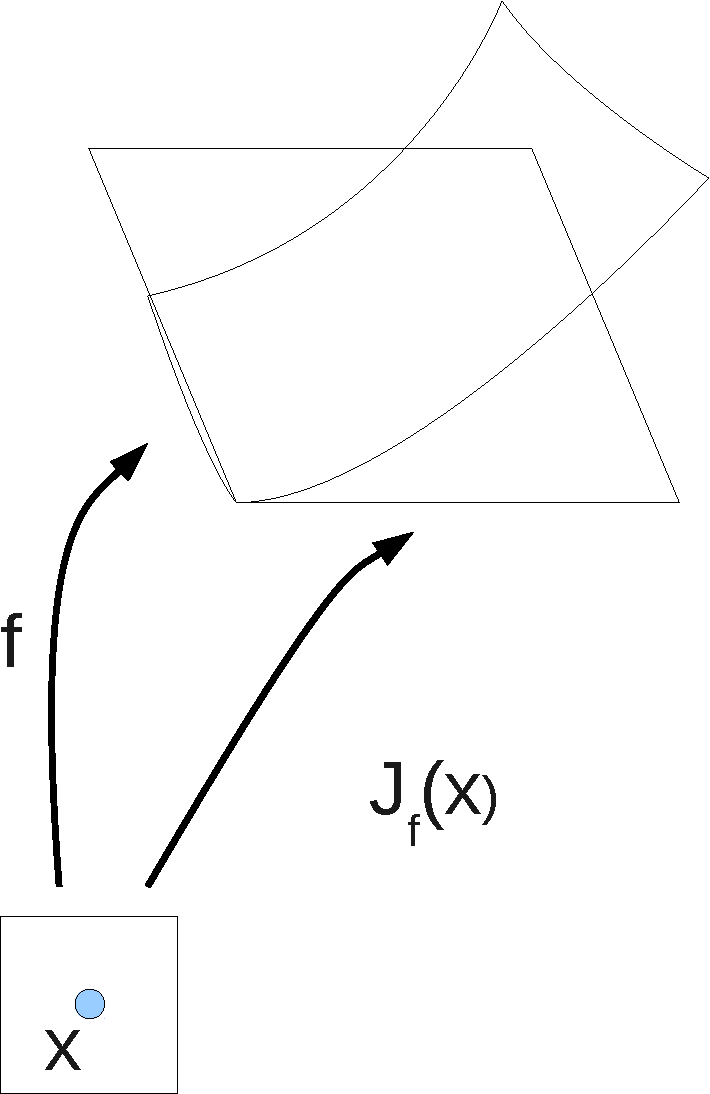
\includegraphics[scale=0.3]{images/jacobien.pdf}
\caption{Volume image et volume image approché}\label{ch3:2}
\end{figure}
La proposition suivante va prouver
que dans le cas simple des cubes, la différence entre les deux peut être bornée, 
et rendue aussi petite que l'on souhaite en restreignant
la taille des cubes considérés. 
\begin{prop}
Soit $U,V$ deux ouverts de $\mathbb{R}^n$ et $K$ un compact de $U$. Soit $f : U \to V$ un
$C^1$-difféomorphisme. Pour tout $\epsilon > 0$, il existe $\delta >
0$ tel que pour tout cube $C$ de centre $x_0 \in K$ dont la longueur du
côté est inférieure à $\delta$~:
\[
(1-\epsilon)^n |J_f(x_0)| \lambda(C) \leq \lambda(f(C)) \leq (1+\epsilon)^n
|J_f(x_0)| \lambda(C)
\]
\end{prop}
\begin{proof}
Par hypothèse, $f^\prime$ est continue, il existe donc $\delta > 0$
tel que~:
\[
\| x - x_0 \| < \delta \rightarrow \| f^\prime(x) - f^\prime(x_0) \| < \epsilon
\]
On peut choisir $\delta$ suffisamment petit pour que  $C \subset K$
et que la propriété ci-dessus soit vraie. 
Pour tout $x \in C$, il existe $c \in C$ tel que $f(x) - f(x_0) =
f^\prime(c) (x-x_0)$. En combinant ce résultat avec le précédent, on
en déduit~:
\[
\| f(x) - f(x_0) - f^\prime(x_0)(x-x_0)\| \leq \epsilon \|x-x_0\|
\]
Soit l'application affine~:
\[
T : x \to f(x_0)+f^\prime(x_0)(x-x_0)
\]
On peut écrire, pour $x \in C$~:
\[
f(x) = T(x + T^{-1}g(x,x_0))
\]
avec $\| g(x,x_0) \| \leq \epsilon \|x -x_0\|$.
En posant~:
\[
\eta = \sup \{ \| f^{\prime}(x)^{-1} \|, x \in K \}
\]
il vient~:
\[
\|  T^{-1}g(x,x_0) \| \leq \eta \epsilon \| x - x_0 \|
\]
et donc~:
\[
\lambda(f(C)) \leq \lambda(T((1+\eta \epsilon )C)) =
(1+\eta\epsilon)^n |J_f(x_0)| \lambda(C)
\]
On montrerait de même la minoration.
\end{proof}
\begin{defn}
Un cube élémentaire d'ordre $k \geq 1$ est un cube de la forme~:
\[
C = \prod_{i=1}^n [ x_i 2^{-k}, (x_i + 1)2^{-k} ]
\]
où les $x_i, i=1\dots n$ sont des entiers.
\end{defn}
En recouvrant un cube élémentaire $C$ d'ordre $k$ quelconque par des
cubes vérifiant les hypothèses de la proposition précédente pour
$\epsilon > 0$ donné, on obtient (exercice)~:
\[
(1-\epsilon)^2 \int_{C} |J_f(x)|d \lambda(x) \leq \lambda(f(C)) \leq
(1+\epsilon)^2 \int_{C} |J_f(x)| d \lambda(x)
\]
puis l'égalité par passage à la limite. 
\begin{mandatory}
\begin{prop}
Soient $U,V$ ouverts de $\mathbb{R}^n$. Soit $f : U \to V$ un
$C^1$-difféomorphisme. On a, pour tout borélien $B$~:
\[
\lambda(f(B)) = \int_B |J_f(x) |d \lambda(x)
\]
\end{prop}
\end{mandatory}
\begin{proof}
Les cubes élémentaires d'adhérence incluse dans $U$ forment une
classe monotone $\mathcal{C}$. La mesure  $\lambda(f(C))$ d'un cube
$C$ de cette classe est égale à $ \int_C |J_f(x) |d \lambda(x)$. Le
résultat se déduit du théorème des classes monotones en remarquant que
$\mathcal{C}$ est stable par intersections finies et engendre la tribu
de Borel.
\end{proof}
\begin{rem}
 L'extension de la proposition au cas des $C^1$-difféo\-morphismes par
morceaux se fait immédiatement en l'appliquant sur une partition de
$U$.
\end{rem}
\begin{mandatory}
\begin{prop}{(Changement de variable)}
Sous les hypothèses précédentes, on a, pour toute application $g : V
\to \mathbb{R}$~:
\[
\int_V g(x) d \lambda(x) = \int_U g(f(x)) |J_f(x)| d \lambda(x)
\]
\end{prop}
\end{mandatory}
\begin{rem}
La proposition est une conséquence immédiate du résultat sur la mesure
image. Pour une application $g$ de signe quelconque, on utilisera souvent
la formule ci-dessus sur $|g|$ pour montrer la sommabilité, puis à
nouveau sur $g$ pour calculer l'intégrale (en toute rigueur pour
$g^+,g^-$, mais un calcul élémentaire montre que cela revient au même).
\end{rem}
La technique du changement de variable est à connaître absolument: c'est une
des méthodes de base pour calculer une valeur d'intégrale.
\begin{exercice}
Soit l'application $f : \mathbb{R}^{+2} \to \mathbb{R}^+$ définie par~:
\[
f : (x,y) \to e^{-x^2 -y^2}
\]
\begin{itemize}
\item A l'aide du changement de variable~:
\[
\begin{array}{c}
x = \rho \cos \theta \\
y = \rho \sin \theta 
\end{array}
\]
où $\rho \in \mathbb{R}^+, \, \theta \in [0, \frac{\pi}{2}]$, calculer~:
\[
\int_{\mathbb{R}^{+2}} f(x,y) d \lambda(x) \times d \lambda(y)
\]
\item En déduire la valeur de~:
\[
\int_{\mathbb{R}} e^{-x^2} d \lambda (x)
\]
\end{itemize}
\end{exercice}
L'utilisation conjointe des théorèmes de Fubini-Tonnelli et du changement de
variable est fréquente. Dans l'exercice suivant, on établit une relation entre
des fonctions appelées fonctions eulériennes gamma et béta, qui sont d'un usage
assez courant.
\begin{exercice}
Soit $a>0, b>0$ deux réels strictement positifs. 
\begin{itemize}
  \item Montrer que les deux intégrales
suivantes sont bien définies:
\[
\Gamma(a) = \int_{\mathbb{R}^+} e^{-x}x^{a-1} d\lambda(x) \, , \, B(a,b) =
\int_{[0,1]} x^{a-1}(1-x)^{b-1} d \lambda(x)
\]
\item Montrer que:
\[
\Gamma(a) = 2 \int_{\mathbb{R}^+} e^{-x^2} x^{2a-1} d \lambda(x)
\]
\item Justifier avec précision que:
\[
\Gamma(a)\Gamma(b) = 4 \int_{\mathbb{R}^{+2}}
e^{-(x^2+y^2)}x^{2a-1}y^{2a-1}d\lambda(x) d\lambda(y)
\]
\item En utilisant le changement de variable de l'exercice précédent, en
déduire:
\[
\Gamma(a)\Gamma(b)=B(a,b)\Gamma(a+b)
\]
\end{itemize}

\end{exercice}

% \chapter{Les espaces $L^p$}
\section{Définitions}
Dans ce chapitre, on supposera donné un espace mesuré $(E, \mathcal{T}, \mu)$. 
\begin{defn}
Pour $p \geq 1$ réel, l'ensemble $\mathcal{L}^p_{\mathbb{R}}$ (resp.
$\mathcal{L}^p_{\mathbb{C}}$) est l'ensemble des applications $f: E
\to \mathbb{R}$ (resp.  $f: E \to \mathbb{C}$) telles que~:
\[
\int_E |f|^p d \mu < + \infty
\]
L'ensemble  $\mathcal{L}^\infty_{\mathbb{R}}$ (resp.
$\mathcal{L}^\infty_{\mathbb{C}}$) est l'ensemble des applications $f: E
\to \mathbb{R}$ (resp.  $f: E \to \mathbb{C}$) telles que~:
\[
\exists C > 0 \text{ tel que } |f| \leq C \quad \mu\text{-pp}
\]
\end{defn}
Ces ensembles sont des espaces vectoriels sur $\mathbb{R}$ ou
$\mathbb{C}$, mais ne sont pas d'une grande utilité, deux applications
ne différant que sur un ensemble de $\mu$-mesure nulle ayant les mêmes
propriétés vis à vis de l'intégrale. 
Dans la suite, la notation  $\mathcal{L}^p$ désignera selon le
contexte, et si cela ne pose aucune difficulté, aussi bien
$\mathcal{L}^p_{\mathbb{R}}$ que $\mathcal{L}^p_{\mathbb{C}}$.
\begin{prop}
Soit $1 \leq p \leq +\infty$. Dans l'ensemble $\mathcal{L}^p$ la
relation~:
\[
(f \mathcal{R} g) \Leftrightarrow (f = g \quad \mu\text{-pp})
\]
est une relation d'équivalence. La classe d'équivalence de $f$ sera
notée $[f]$.
\end{prop}
\begin{mandatory}
\begin{defn}
Pour $+\infty \geq p \geq 1$, on pose~:
\[
L^p = \mathcal{L}^p / \mathcal{R}
\]
\end{defn}
\end{mandatory}
En vertu de la proposition \ref{ch2:upp}, toutes les applications d'une même
classe d'équivalence ont même intégrale de Lebesgue: on pourra ainsi parler de
l'intégrale d'une classe d'équivalence ou par abus de language de l'intégrale
d'une fonction de $L^p$.

Les ensembles $L^p$ peuvent être munis d'une structure d'espace vectoriel en posant, pour $\mathbb{K} =
\mathbb{R}$ ou $\mathbb{K} = \mathbb{C}$~:
\begin{align*}
& \forall f \in L^p , \, \forall \lambda \in \mathbb{K}, \, \lambda [f] =
  [\lambda f] \\
& \forall f \in L^p, \forall g \in L^p, \, [f] + [g] = [f+g]
\end{align*}


On vérifie également simplement que l'on peut poser, pour toute
application $f \in \mathcal{L}^p$~: $|[f]| = [|f|]$.

Dans la suite, on confondra le plus souvent une classe d'équivalence
avec un représentant, et on parlera de fonction de $L^p$, étant entendu que l'on
travaille en fait sur la classe contenant la fonction.

L'intérêt majeur des espaces $L^p$ est qu'ils peuvent être munis d'une norme.
Pour $f \in L^p, p < +\infty$ (on confond ici comme annoncé représentant avec classes d'équivalence), on posera~:
\[
\| f\|_p = \left ( \int_E |f|^p d \mu \right )^{1/p}
\]
et pour $f\in L^\infty$~:
\[
\|f\|_\infty = \inf \{ C > 0 \text{ tel que } |f(x)| \leq C \mbox{ pour } \mu
\mbox{-presque tout } x \}
\]
On a de façon évidente~:
\begin{itemize}
\item $\|f\|_p = 0 \Leftrightarrow f = 0$. Cette égalité n'est vraie que dans $L^p$ et non dans $\mathcal{L}^p$.
\item $\| \lambda f \|_p = |\lambda| \| f \|$ pour tout $\lambda \in \mathbb{R}$ (resp. $\lambda \in \mathbb{C}$).
\end{itemize}
L'inégalité triangulaire est encore à vérifier, ce qui va être l'objet des développements suivants.
\begin{mandatory}
\begin{theorem}{(Inégalité de Hölder)}
Soit $p \in[1, +\infty]$. Soit $f \in L^p, g\in L^q$ avec $p^{-1}+q^{-1} = 1$ (on dit que $p$ et $q$ sont conjugués). On a~:
\begin{itemize}
\item $fg \in L_1$.
\item $\|fg\|_1 \leq \|f\|_p \|g\|_q$.
\end{itemize}
\end{theorem}
\end{mandatory}
\begin{proof}
Si $p=1, q=\infty$, on écrit simplement~:
\[
\int_E |fg|d \mu \leq \int_E \|g\|_\infty |f| d \mu = \|g\|_\infty \|f\|_1
\]
Supposons donc que $+\infty > p > 1$.
Soit, pour $\alpha \in ]0,1[$, l'application $x>0 \to x^\alpha -
    \alpha x$. Elle est maximale pour $x=1$ d'où~: $\forall x > 0 ,
    x^\alpha - \alpha x \leq 1 - \alpha$.  En considérant un $x$ de la
    forme $\frac{u}{v}$, il vient~:
\[
u^\alpha v^{1-\alpha} \leq \alpha u +(1-\alpha)v
\]
On peut supposer $\|f\|_p>0, \|g\|_q> 0$ car sinon la proposition est évidente.
En prenant $\alpha = p^{-1}$ et~:
\[
\begin{array}{cc}
u = \frac{|f|^p}{\|f\|_p^p} & v = \frac{|g|^q}{\|g\|_q^q}
\end{array}
\]
on a~:
\[
\frac{|fg|}{\|f\|_p\|g\|_q} \leq \frac{|f|^p}{p \|f\|_p^p} +
\frac{|g|^q}{q \|g\|_q^q}
\]
qui conduit par intégration des deux membres de l'inégalité au
résultat recherché.
\end{proof}
L'intérêt de l'inégalité de Hölder va bien au delà de la preuve de l'inégalité
de Minkowsky qui sera vue ci-dessous. Si $p,q$ sont des exposants conjugués,
elle montre que l'intégrale définit sur $L^p \times L^q$ une forme bilinéaire
continue (ou sesquilinéaire continue en complexe).

\begin{mandatory}
 \begin{theorem}{(Inégalité de Minkowsky)}
Soit $p\in [1,+\infty]$ et $f,g \in L^p$. Alors $f+g \in L_p$ et
$\|f+g\|_p \leq \|f\|_p + \|g\|_p$.
\end{theorem}
\end{mandatory}
\begin{proof}
Comme précedemment, les cas $p=1$ et $p=\infty$ sont immédiats. On
supposera donc $+\infty > p > 1$. L'application $x>0 \to x^p$ est
convexe, donc~:
\[
\frac{|f+g|^p}{2^p} \leq \frac{|f|^p + |g|^p}{2}
\]
ce qui prouve que $f+g \in L^p$. En écrivant~:
\[
|f+g|^p =
|f+g||f+g|^{p-1} \leq |f| |f+g|^{p-1} + |g||f+g|^{p-1}
\]
et en intégrant cette inégalité, on obtient~:
\[
\int_E |f+g|^p d \mu \leq \int_E |f||f+g|^{p-1} d \mu + \int_E
|g||f+g|^{p-1} d \mu
\]
L'inégalité de Hölder s'applique aux deux termes du membre de droite avec les
exposants $p,q=p/(p-1)$~:
\[
\int_E |f+g|^p d \mu \leq \|f\|_p \left (\int_E |f+g|^p d \mu \right)
^{\frac{p-1}{p}}
+ \|g\|_p \left (\int_E |f+g|^p d \mu \right )^{\frac{p-1}{p}}
\]
Si $\int_E |f+g|^p d \mu =0$, la proposition est immédiate. Sinon, le
résulat est obtenu en divisant l'inégalité par $ \left (\int_E |f+g|^p d \mu \right )^{\frac{p-1}{p}}$.
\end{proof}
Ce dernier théorème montre que $\|\|_p$ est une norme.
\section{Propriété des espaces $L^p$}
\begin{mandatory}
\begin{theorem}
Munis de la norme $\|\|_p$, les espaces $L^p, p\in [1,+\infty]$ sont complets.
\end{theorem}
\end{mandatory}
\begin{proof}
Le cas $p=\infty$ est simple. Supposons $p < +\infty$. Soit $(f_n)$
une suite de Cauchy dans $L^p$. On peut en extraire une sous-suite
$(g_k)$ telle que $\forall k \in \mathbb{N}, \|g_{k+1}-g_k\|_p \leq
2^{-k}$.
Le théorème de convergence monotone montre immédiatement que~:
\[
\int_E \left ( \sum_{n \geq 1} | g_{n+1} - g_n | \right )^p d
\mu = \lim_{k \to +\infty}  \int_E \left ( \sum_{n=1}^k | g_{n+1} - g_n
| \right )^p d \mu
\]
En appliquant l'inégalité de Minkowsky, le second membre de l'égalité
se majore par~:
\[
\lim_{k \to +\infty}  \left ( \sum_{n=1}^k \| g_{n+1} - g_n \|_p
\right )^p = \left ( \sum_{n \geq 1} \| g_{n+1} - g_n \|_p
\right )^p
\]
qui est une quantité finie.
L'application~:
\[
h = g_1 + \sum_{k\geq 1} (g_{k+1} - g_k)
\]
est donc définie $\mu$-presque partout. Comme $(g_n)$ converge
$\mu$-presque partout vers $h$, le lemme de Fatou donne~:
\[
\int_E |h|^p d \mu \leq \liminf_n \int_E |g_n|^p d \mu 
\]
Le membre de droite est fini car la suite $(g_n)$ est une sous-suite
de la suite $(f_n)$ qui, étant de Cauchy, est bornée.
Ceci prouve que $h \in L^p$. Enfin, pour tout entier $n$~:
\begin{align*}
\int_E | h - g_n|^p d \mu & \leq \liminf_k \int_E |g_k -g_n|^p d \mu
\\
& \leq \left ( \sum_{i=n}^{k-1} \| g_{i+1} - g_i \|_p \right )^p \\
& \leq
\left (2^{-n+1} \right)^p
\end{align*}
qui tend vers 0 pour $n \to +\infty$. On en déduit $g_n \to h$ dans
$L^p$, donc $f_n \to h$ dans $L^p$ et la proposition est prouvée.
\end{proof}
Ce théorème est extrêmement important en pratique et n'a pas
d'équivalent en intégration de Riemann. 
\begin{prop}\label{ch3:p1}
Dans un espace mesuré $(E, \mathcal{T}, \mu)$ avec $\mu(E) < +\infty$,
on a $L^q \subset L^p$ si $1 \leq p \leq q \leq +\infty$.
\end{prop}
\begin{proof}
$\mu$ étant une mesure finie, l'application constante $1$ est sommable
(elle appartient de fait à tous les espaces $L^p$). Soit $f \in
L^p$. L'inégalité de Hölder appliquée au produit $|f|^{p} 1$ donne~:
\begin{align*}
\int_E |f|^p d \mu & \leq \left ( \int_E 1 d \mu \right ) ^{\frac{q}{q-p}}
\|f\|_q \\ & \leq \mu(E)^{\frac{q}{q-p}} \|f\|_q < +\infty
\end{align*}
\end{proof}
\begin{rem}
Rien ne subsiste si $\mu$ n'est pas finie, il faut donc prendre garde à ce que
l'on écrit, comme le montre l'exercice suivant.
\end{rem}
\begin{exercice}
Soit l'application $f : \mathbb{R} \to \mathbb{R}$ définie par~:
\[
\forall x \in \mathbb{R}, \, f(x) = \left \{
\begin{array}{cc}
0 & \mbox { si } < \leq 0 \\
\frac{1}{x(1+ln^2(x))} & \mbox{ sinon }
\end{array}
\right .
\]
\begin{itemize}
\item Montrer que $f$ est sommable.
\item Montrer que $ \forall p > 1, \, f \notin L^p$.
\item En déduire qu'il existe pour tout $p \in [1, +\infty[$ une application $f$ telle que 
$f\in L^p, \, f \notin  L^q, \, q \in  [1, +\infty[, \, q \neq p$.
\end{itemize}
\end{exercice}
Toujours dans le cas des mesures finies, il existe une interprétation de la
notation un peu surprenante $L^\infty$. 
\begin{exercice}
Soit $(E,\mathcal{T},\mu)$ un espace mesuré avec $\mu(E) < +\infty$.
\begin{itemize}
\item Montrer que~:
\[
(f \in L^\infty) \Leftrightarrow \left(\forall p \in [1, +\infty[, \, 
f \in L^p \mbox { et } \sup_p \| f\|_p < +\infty\right)
\]
\item Si ces conditions sont vérifiées, montrer que $\lim_{p \to +\infty}
\|f\|_p = \|f\|_\infty$.
\end{itemize}
\end{exercice}
\begin{theorem}
Pour $p \in [1,+\infty[$, Les applications étagées sont denses dans $L^p$.
\end{theorem}
\begin{proof}
Il suffit de montrer la proposition pour une application $f \in L^p$ réelle positive, le cas
général en decoulant en décomposant une application de $L^p$
quelconque en partie positive et négative (et partie rélle et
imaginaire si $f$ est à valeurs complexes). 
$f$ est limite simple d'une suite croissante $(g_n)$ d'applications étagées
(voir proposition\ref{ch2:1}). Comme pour tout $n$, $g_n \leq f$, on a
également~:
\[
\int_E |g_n|^p d \mu \leq \int_E |f|^p d \mu < +\infty
\]
d'où $\forall n, g_n \in L^p$. Par ailleurs, $\forall n, |f- g_n|^p
\leq 2^p f^p$, donc le théorème de convergence dominée s'applique et l'on
a~:
\[
\lim_n \|f-g_n\|^p = \lim_n \int_E |f - g_n|^p d \mu = 0
\]
\end{proof}
Dans le cas où la mesure $\mu$ vérifie des conditions supplémentaires,
il est possible d'obtenir un résultat de densité pour des applications
plus régulières que les applications étagées.  
\begin{prop}
Soit $E$ un espace métrique muni de sa tribu des Boréliens et
  soit $\mu$ une mesure vérifiant la propriété~:
\[
\forall A \in \mathcal{B}(E), \, \mu(A) = \inf \{ \mu(O), O \mbox{
  ouvert }, \, O \supset A \}
\]
alors l'ensemble des applications lipschitziennes bornées est dense dans
$L^p(E, \mathcal{B}(E), \mu)$.
\end{prop}
\begin{proof}
On peut se limiter à prouver que toute indicatrice $1_A$ avec $A \in
\mathcal{B}(E)$  est limite dans $L^p$ d'une suite
d'applications lipschitiziennes bornées. 
Soit $\epsilon > 0$. Il existe par hypothèse un ouvert $O$ tel que $O
\supset a$ et $\mu(O-A) < \epsilon$. On en déduit~:
\[
\| 1_O - 1_A \|_p^p < \epsilon
\]
Soit pour tout entier $k$ l'application lipschitzienne ~: 
\[
g_k(x) = \min(k d(x, O^c), 1) 
\]
On a $\lim g_k \to 1_O$ et, par le théorème de convergence dominée~:
\[
\lim_k \int_E |1_O -g_k|^p d \mu \to 0
\]
donc il existe $k_0$ tel que~:
\[
\forall k \geq k_0 \, , \, \| 1_0 - g_k \|_p^p < \epsilon
\]
La suite $(g_k)$ converge ainsi dans $L^p$ vers $1_A$ et la proposition est prouvée.
\end{proof}
\section{L'espace $L^2$}
L'exposant $2$ est conjugué à lui-même. La forme bilinéaire (resp.
sesquilinéaire) donnée par l'inégalité de Hölder va induire un produit scalaire
sur cet espace. Associé à la complétude, le caractère Hilbert de $L^2$
s'ensuivra.
\begin{mandatory}
\begin{prop}
L'espace $L^2$ muni du produit scalaire~:
\[
\langle f, g \rangle = \int_E f \overline{g} d \mu
\]
est un espace de Hilbert.
\end{prop}
\end{mandatory}
Le caractère Hilbert de $L^2$ permet d'utiliser quelques théorèmes très
puissants comme l'existence d'une projection orthogonale ou le théorème de
représentation de Riesz. Ces deux résultats sont rappelés ci-dessous:
\begin{mandatory}
\begin{theorem}
Soit $H$ un espace de Hilbert et soit $C \subset H$ une partie convexe fermée
non vide de $H$. Pour tout $x \in H$, il existe un unique point $\tilde{x} \in
C$ tel que $\forall y \in C, \, \|x-\tilde{x}\| \leq \|x-y\|$. 
Dans le cas où $C$ est un sous-espace vectoriel fermé de $H$, ce point est
caractérisé par la propriété suivante:
\[
\forall y \in C, \, \langle x - \tilde{x}, y - \tilde{x}\rangle=0
\]
\end{theorem}
\end{mandatory}
La démonstration n'est pas rappelée ici, mais utilise une suite de Cauchy
de points de $C$ convergeant vers $\tilde{x}$: le caractère fermé et complet de
$C$ est absolument nécessaire. Le point $\tilde{x}$ est appelé projection
orthogonale de $x$ sur $C$.
\begin{mandatory}
\begin{theorem}(Théorème de représentation de Riesz)
Soit $H$ un espace de Hilbert et soit $\phi \colon H \to \mathbb{R}$ (resp.
$\phi \colon H \to \mathbb{C}$) une forme linéaire \textbf{continue} sur $H$. Il
existe un unique vecteur $v \in H$ tel que:
\[
\forall x \in H, \, \phi(x) = \langle x, v \rangle
\]
\end{theorem}
\end{mandatory}
\begin{proof}
La forme $\phi$ étant continue, son noyau $\ker \phi = \phi^{-1}(0)$ est un
sous-espace vectoriel fermé de $H$. Pour tout $x\in H$, on note $p(x)$ sa
projection orthogonale sur $\ker \phi$ (elle existe en vertu du théorème
précédent). L'écriture $x = (x-p(x)) + p(x)$ montre que $\ker \phi$ possède un
supplémentaire orthogonal $H_1$ dans $H$. $H_1$ est de dimension $1$
($\phi|_{H_1}$ est inversible), donc est engendré par un vecteur non nul $e$
tel que $\phi(e) \neq 0$. Pour tout $x \in H$, peut ainsi écrire $x = \lambda e
+ y$, $y \in \ker \phi$ et $\lambda$ un scalaire. On note que $\phi(x) =
\lambda \phi(e)$ et que $\langle x, e,\rangle  = \lambda \langle e, e \rangle$.
Le vecteur $v$ de la proposition est donc:
\[
v = e \frac{\phi(e)}{\langle e, e \rangle}
\]
\end{proof}
Le théorème de représentation de Riesz, appliqué à $L^2$, permet de prouver de
façon élégante un résultat d'une grande importance en théorie des probabilités.
\begin{defn}
Soit $(E, \mathcal{T})$ un espace mesurable et soient $\mu, \nu$ deux
mesures sur $E$. On dira que $\nu$ est absolument continue par rapport
à $\mu$ (noté $\nu \ll \mu$) si pour toute partie $A \in \mathcal{T}$,
$\mu(A) = 0 \Rightarrow \nu(A) = 0$. De même, on dira que $\nu$ est
étrangère à $\mu$ (noté $\nu \perp \mu$) si il existe $A \in
\mathcal{T}$ avec $\mu(A) = 0$ et $\nu(A^c) = 0$.
\end{defn}
Une forme très importante de mesure absolument continue est donnée par la proposition ci-dessous.
\begin{mandatory}
\begin{prop}
Soit $(E, \mathcal{T}, \mu)$ un espace mesurable
et soit  $f$ une application positive sommable définie sur $E$. On pose pour
tout $A$ mesurable:
\[
\mu_f(A) = \int_{A} f(x) d \mu(x)
\]
Alors $\mu_f$ est une mesure absolument continue par rapport à $\mu$.
\end{prop}
\end{mandatory}
\begin{proof}
$\mu_f(\emptyset)=0$ de façon évidente et si $(A_n)_{n \in \mathbb{N}}$ est une
famille disjointe de parties $\mu$-mesurables, alors:
\[
\mu_f\left(\bigcup_{n \in \mathbb{N}} A_n \right) = \int_{\mathbb{R}} \sum_{n
\in \mathbb{N}} 1_{A_n} f(x) d \mu(x)
\]
Par le théorème de convergence dominée, il vient:
\[
 \int_{\mathbb{R}} \sum_{n
\in \mathbb{N}} 1_{A_n} f(x) d \mu(x) = \lim_{k \to +\infty}
\int_{\mathbb{R}} \sum_{n=0}^k 1_{A_n} f(x) d \mu(x)
\]
Soit avec la relation de Chasles:
\[
\int_{\mathbb{R}} \sum_{n
\in \mathbb{N}} 1_{A_n} f(x) d \mu(x) = \lim_{k \to +\infty}
\sum_{n=0}^k \int_{A_n} f(x) d \mu(x) = \lim_{k \to +\infty}
\sum_{n=0}^k \mu_f(A_n)
\]
qui prouve l'additivité dénombrable.
Soit $\epsilon > 0$. Le théorème de convergence monotone donne:
\[
\lim_{n \to +\infty} \int_{\mathbb{R}} f\wedge n(x) d \mu(x) = 
\int_{\mathbb{R}} f(x) d \mu(x)
\] 
Il existe donc $n_\epsilon$ tel que pour tout $n \geq n_{\epsilon}$:
\[
\int_{\mathbb{R}} f(x) d \mu(x) - int_{\mathbb{R}} f\wedge n(x) d \mu(x)
< \frac{\epsilon}{2}
\]
Soit $A$ une partie $\mu$-mesurable telle que:
$$\mu(A) < \frac{\epsilon}{2n_\epsilon}$$
On a, pour tout $n \geq n_{\epsilon}$:
\[
\int_{A} f(x)d \mu(x) < \int_{A} f \wedge n(x) d \mu(x) +
\frac{\epsilon}{2} < n \mu(A) + \frac{\epsilon}{2}  < \epsilon
\]
\end{proof}
Le théorème de Radon-Nikodym énoncé ci-dessous va établir une forme de
réciproque.
\begin{mandatory}
\begin{theorem}{(Radon-Nikodym)}
Soit $\mu, \nu$ deux mesures $\sigma$-finies sur un espace mesurable $(E,
\mathcal{T})$. Il existe un unique couple $(\nu_a, \nu_s)$ de mesures
finies sur $(E, \mathcal{T})$ tel que~:
\begin{itemize}
\item $\nu = \nu_a + \nu_s$;
\item $\nu_a \ll \mu, \, \nu_s \perp \mu$;
\item $\nu_a = f \mu$, $f$ application sommable sur
$E$.
\end{itemize}
\end{theorem}
\end{mandatory}
\begin{proof}
On suppose dans un premier temps que les mesures sont finies et que
pour toute application positive sommable $f$~: 
\[
\int_E f d \nu \leq \int_E f d \mu
\]
Pour $f \in L^2(\mu)$, on pose~:
\[
P(f) = \int_E f d \nu
\]
Cette quantité est bien définie car $\nu$ finie implique $L^2(\nu) \subset
L^1(\nu)$ en vertu de la proposition \ref{ch3:p1} et par hypothèse~:
$\|f\|_{L^2(\nu)} \leq \|f\|_{L^2(\mu)}$. Par ailleurs,
l'inégalité de Hölder donne~:
\[
|P(f)| \leq \sqrt{\nu(E)} \|f\|_{L^2(\mu)}
\]
$P$ est donc une forme linéaire continue sur $L^2(\mu)$, espace de
Hibert. Le théorème de représentation de Riesz montre qu'il existe une
application $g \in L^2(\mu)$ telle que ~:
\[
\forall f \in L^2(\mu), \, P(f) = \int_E f g  d \mu
\]
et l'on a, pour toute partie mesurable $A$~:
\[
\nu(A) = \int_E 1_A g d \mu
\]
L'application $g$ peut être choisie de telle sorte qu'elle prenne ses
valeurs dans $[0,1]$. En effet, pour tout $\epsilon > 0$~:
\begin{align*}
&\nu(\{x | g(x) < - \epsilon \})
\leq -\epsilon \mu(\{x| g(x) < - \epsilon \}) \\
&\mu(\{x | g(x) > 1 + \epsilon \}) \geq \nu(\{x | g(x) > 1 + \epsilon
\}) \geq \\
& (1+\epsilon) \mu(\{x | g(x) > 1 + \epsilon \})
\end{align*}
d'où~:
\[
\mu(\{x | g(x) < - \epsilon \}) = \mu(\{x | g(x) > 1 + \epsilon \}) = 0
\]
En revenant au problème initial et toujours dans l'hypothèse de
mesures finies, on peut appliquer le développement
précédent aux mesures $\nu, \nu+\mu$. Pour toute application mesurable
bornée $f$ il existe une application $g$ avec~:
\[
\int_E f d \nu = \int_E f g d \mu + \int_E f g d \nu
\]
soit~:
\[
\int_E f (1-g) d \nu = \int_E fg d \mu 
\]
résultat s'étendant à toute appplication mesurable positive par le
théorème de convergence monotone. 
L'ensemble $N = \{ x | g(x) = 1 \}$ est de $\mu$-mesure nulle (faire
$f=1_N$ dans l'égalité précédente). On obtient alors les mesures~:
\begin{align*}
& \nu_s = 1_N \nu \\
& \nu_a = 1_{N^c} \nu
\end{align*}
avec, pour tout $A$ mesurable~:
\[
\nu_a(A) = \int_E 1_{A \cap N^c} \frac{g}{1-g} d \mu
\]
L'unicité s'obtient de façon simple. Pour le cas $\sigma$-fini,
appliquer le résultat précédent sur un recouvrement dénombrable de $E$ par des
ensembles de mesure finie.
\end{proof}
Enfin, il faut terminer ce développement en mentionnant la relation existant
entre intégrale et primitive dans le cadre de la théorie de Lebesgue.
\begin{mandatory}
\begin{theorem}\label{thm:derivee_integrale}
Soit $f$ une application sommable. On pose pour tout $x \in \mathbb{R}$:
\[
F(x) = \int_{]-\infty,x]} f(t) d \lambda(t)
\]
alors pour presque tout $x \in \mathbb{R}$, l'application $F$ est dérivable en
$x$ de dérivée est égale à $f(x)$.
\end{theorem}
\end{mandatory}
Cette proposition justifie le calcul d'une intégrale par une primitive, sous
réserve bien sûr qu'elle puisse être exhibée dans ce cadre plus général. La
preuve de cet énoncé simple en apparence est étonnamment difficile. Plusieurs
lemmes intermédiaires sont nécessaires avant de pouvoir conclure. Le premier est
dû à F. Riesz et porte le nom évocateur de lemme du soleil levant.
\begin{lemme}\label{lem:soleil_levant}
Soit $f : \mathbb{R} \to \mathbb{R}$ une application continue telle que
$\lim_{x \to +\infty} f(x) = - \infty$, $\lim_{x \to -\infty} f(x) = +\infty$.
L'ensemble:
\[
\mathcal{A} = \{ x | \exists y > x , f(y) > f(x) \}
\]
est ouvert et s'écrit sous la forme d'une union dénombrable d'intervalles
ouverts bornés:
\[
\mathcal{A} = \cup_{i \in \mathbb{N}} ]a_i,b_i[
\]
avec $f(a_i)=f(b_i)$ pour tout entier $i$.
\end{lemme}
Le nom du lemme provient du fait que l'ensemble $\mathcal{A}$ contient tous les
points du graphe de $f$ qu'un observateur situé en $+\infty$ ne pourrait pas
voir, car masqués par d'autres points ou encore tous les points qui ne seraient
pas éclairés par le soleil levant ! La situation décrite par le lemme est
représentée en figure \ref{fig:rising_sun}

\begin{center}
\begin{figure}[ht]
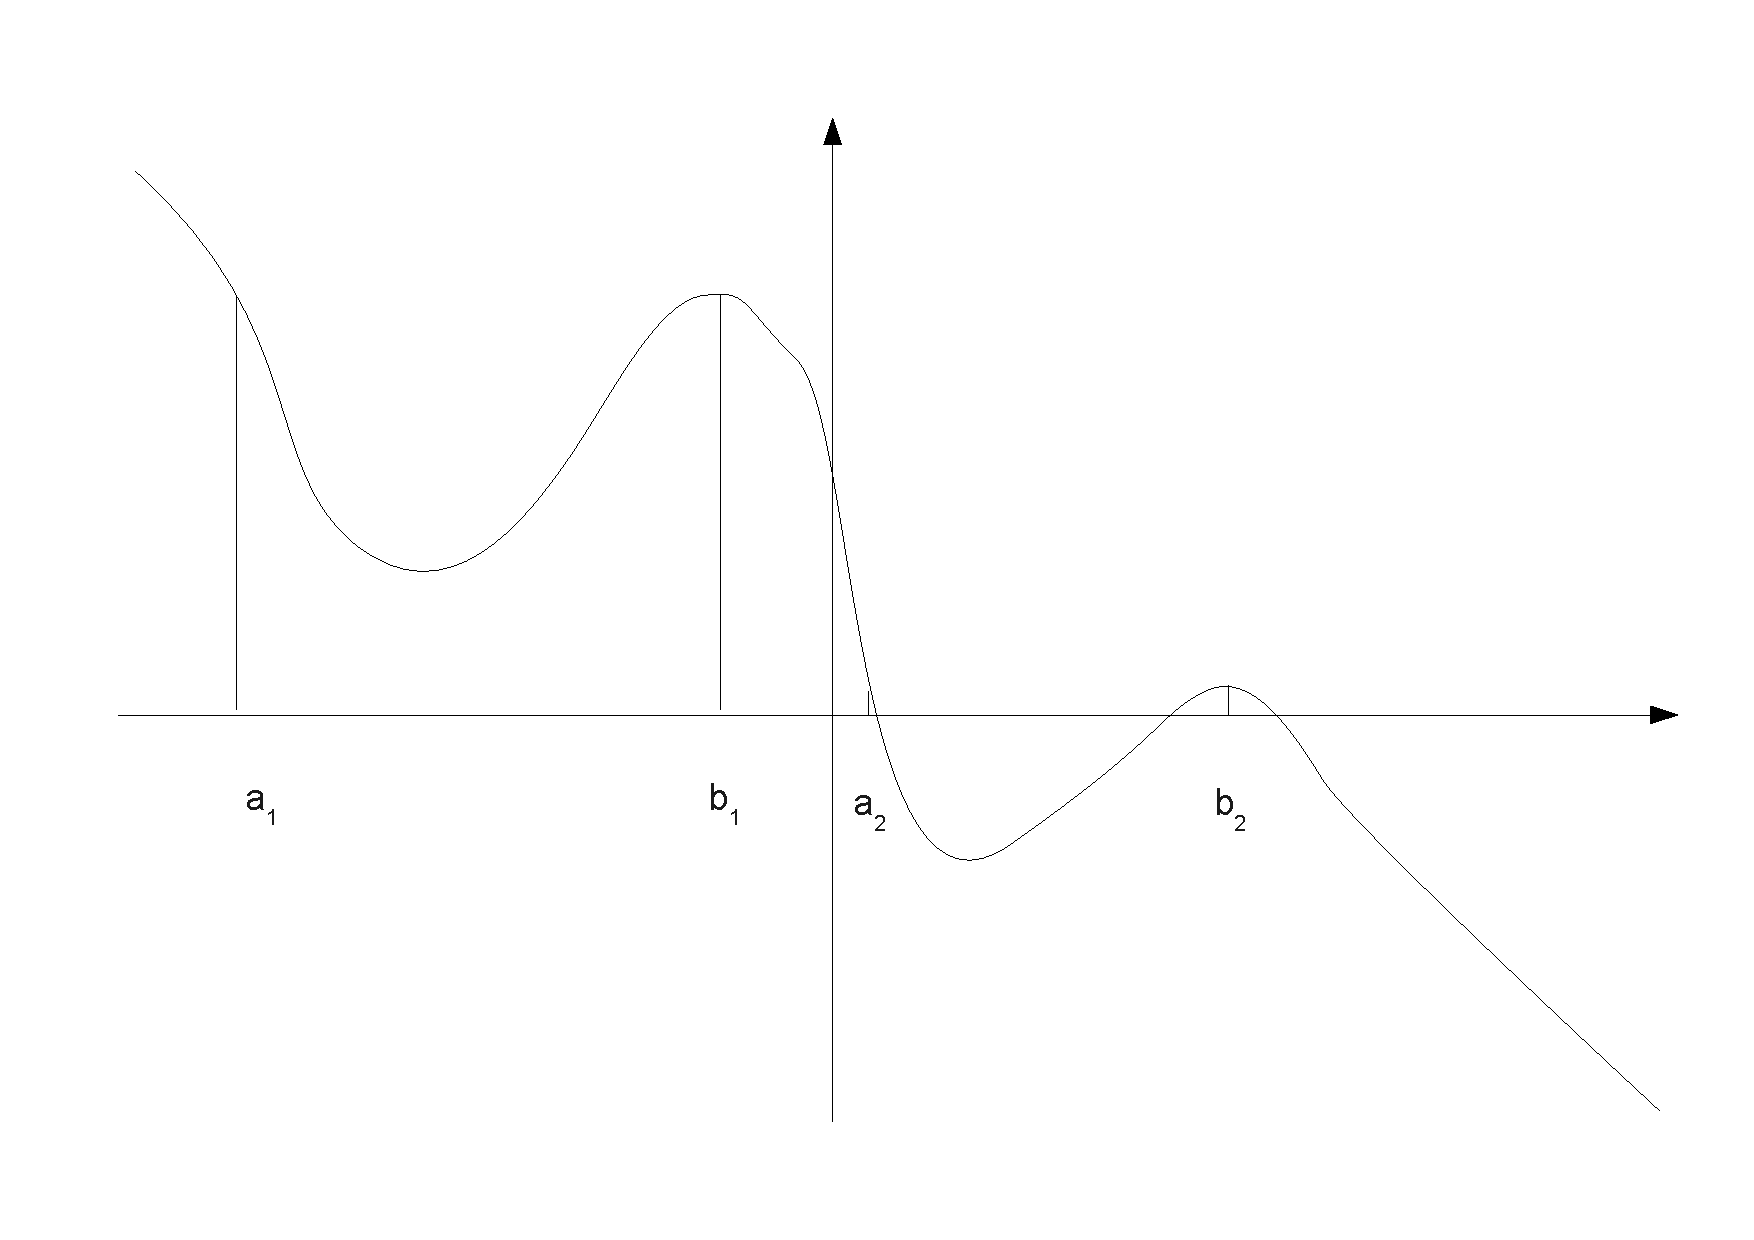
\includegraphics[scale=0.3]{images/rising_sun.pdf}
\caption{Lemme du soleil levant}\label{fig:rising_sun}
\end{figure}
\end{center}

\begin{proof}
Montrons en premier lieu que $\mathcal{A}$ est ouvert. Soit $x \in \mathcal{A}$.
Il existe $y > x$ tel que $f(y) > f(x)$. Soit $\delta = f(y)-f(x)$.
Les points de l'intervalle $I=]f(x)-\delta/2, f(x)+\delta/2[$ sont inférieurs à
$f(y)$. Par continuité de $f$ en $x$, il existe un intervalle ouvert
$J=]x-\epsilon, x+\epsilon[$ tel que $f(J) \subset I$. Quite à réduire
$\epsilon$, on peut supposer que tous les points de $J$ sont inférieurs à $y$ et
on a $J \subset \mathcal{A}$ prouvant que ce dernier ensemble est ouvert. Un
résultat de topologie déjà mentionné montre qu'il s'écrit sous la forme d'une
union dénombrable d'intervalles ouverts, la démonstration du lemme se réduit
alors à pouver qu'ils sont tous bornés. Supposons l'existence d'un intervalle
de la forme $]a,+\infty[ \subset \mathcal{A}$. Soit $K$ un réel. Comme $f$ tend
vers $-\infty$ en $+\infty$, il existe un réel $M>a$ tel que pour tout $x > M$ on ait $f(x) <
f(a)-1$. L'ensemble $\{ u > a, \forall x > u, f(x) < f(a)-1\}$ est non vide (il
contient $M$) et admet une borne inférieure $t$. Pour tout $\epsilon > 0$, on a
$f(t+\epsilon) < f(a) - 1$  et par continuité de $f$, $f(t) \leq f(a)-1$, d'où
$t> a$. Par ailleurs:
\[
\forall x \geq t, f(x) \leq f(a)-1
\] 
et donc $t \notin \mathcal{A}$ ce qui est une
contradiction.
Supposons maintenant qu'un intervalle $]-\infty, a[$ soit inclus dans
$\mathcal{A}$. Comme $f$ est continue et a pour limite $-\infty$ en $+\infty$,
il existe un réel $M$ tel que pour tout $x \geq a$ on ait $f(x) < M$. L'ensemble
des $u$ tels que $f(u) \geq M$ est non vide, contenu dans l'intervalle
$]-\infty, a[$. Soit $t$ sa borne inférieure. Par continuité de $f$, $f(t) = M$
et donc $t < a$. Comme par ailleurs:
\[
\forall x > t, f(x) \leq f(t) 
\]
on aboutit à une contradiction.
Finalement, soit $]a,b[$ un intervalle contenu dans $\mathcal{A}$. Par
définition, $a$ n'appartient pas à $\mathcal{A}$ et on a donc $f(a) \geq f(b)$.
Supposons qu'il existe $t$ dans $]a,b[$ tel que $f(t) > f(b)$. Comme $t$ est
dans $\mathcal{A}$, il existe $y > t$ tel que $f(t) < f(y)$. L'ensemble:
\[
\{ y , y > t, f(t) < f(y) \}
\]
est donc non vide. Il est borné car $f$ tend vers $-\infty$ en $+\infty$ et
admet donc une borne supérieure $g$ finie. Par continuité de $f$, $f(g)=f(t)$ et
pour tout $y > g$, on a $f(y) \leq f(g)$. On en déduit que $g \notin
\mathcal{A}$ et donc que $g > b$. Or $f(g)=f(t)> f(b)$, donc $b \in \mathcal{A}$
ce qui est une contradiction. Ceci montre que pour tout $t \in ]a,b[$, $f(t)
\leq f(b)$ et donc par continuité de $f$, $f(a) \leq f(b)$, soit $f(a)=f(b)$.
 \end{proof}
Le lemme suivant est simple à prouver, mais très utile, spécialement en
probabilités et statistique.
\begin{lemme}{Inégalité de Markov}\label{lem:ineg_markov}
Soit $f$ une fonction de $L^1(\mu)$. Pour tout $\epsilon > 0$, on a:
\[
\mu \left \{ x , |f(x)| > \epsilon 
\right \} \leq \frac{\|f\|_{L^1(\mu)}}{\epsilon}
\] 
\end{lemme}
\begin{proof}
La démonstration est très classique et aisée.
On a:
\begin{align*}
\|f\|_{L^1(\mu)} &= \int_{\mathbb{R}}|f(x)| d\mu(x)  \\
& \geq \int_{\left \{ x , |f(x)| > \epsilon \right \}}|f(x)| d\mu(x) > \epsilon
\mu \left \{ x , |f(x)| > \epsilon \right \}  
\end{align*}
La majoration demandée s'en déduit immédiatement. 
\end{proof}
Le dernier ingrédient est une majoration que l'on appelle inégalité de
Hardy-Littlewood. Elle s'applique à une fonction qui représente une
moyenne sur des intervalles: la fonction maximale de Hardy-Littlewood.
\begin{defn}\label{def:hardy_littlewood}
Soit $f \in L^1$. La fonction maximale de Hardy-Littlewood est définie pour tout
$x$ réel comme:
\[
Mf(x) = \sup_{x \in [a,b]} \frac{1}{b-a} \int_{]a,b[} |f(t)| dt
\]
où la borne supérieure est prise sur tous les intervalles contenant $x$.
\end{defn}
\begin{prop}\label{prop:ineg_hardy_littlewood}
Soit $f \in L^1$. Pour tout $\epsilon > 0$:
\[
\lambda \left(\{ x, Mf(x) \geq \epsilon \}\right) \leq \frac{2}{\epsilon}
\|f\|_{L^1}
\]
\end{prop}
Cette proposition est semblable à l'inégalité de Markov, mais demande un peu
plus de travail pour sa preuve. On utilisera le lemme du soleil levant.
\begin{proof}
On note en premier lieu que le problème se simplifie par l'introduction des
fonctions maximales positives et négatives:
\[
M^+f(x)= \sup_{h > 0} \frac{1}{h} \int_x^{x+h} |f(t)| dt, \, M^-f(x)= \sup_{h >
0} \frac{1}{h} \int_{x-h}^x |f(t)| dt
\]
Il est clair que:
\[
\{x , Mf(x) \geq \epsilon \} = \{x , M^+f(x) \geq \epsilon \}\cup \{x , M^-f(x)
\geq \epsilon \}
\]
On va utiliser $M^+f$, le même raisonnement s'appliquant à $M^-f$. Par
définition, si $M^+f(x) > \epsilon$ alors il existe un $h > 0$ tel que:
\[
\int_x^{x+h} |f(t)| dt > \epsilon h
\]
Soit la fonction:
\[
F_\epsilon \colon u \mapsto \int_{]-\infty,u[} |f(t)|dt - \epsilon u
\]
Elle vérifie les conditions du lemme \ref{lem:soleil_levant} (le vérifier !) et
on a $F_\epsilon(x+h) > F_{\epsilon}(x)$. Soit l'ensemble:
\[
\mathcal{A}_\epsilon = \{ x, \exists y > x, F_\epsilon(y) > F_\epsilon(x) \} 
\]
Par le lemme \ref{lem:soleil_levant}, cet ensemble s'écrit comme réunion
dénombrable disjointe d'intervalles ouverts bornés:
\[
\mathcal{A}_\epsilon = \bigcup_{k \in \mathbb{N}}]a_k,b_k[
\]
avec $F_\epsilon(a_k)=F_\epsilon(b_k)$. Cette dernière égalité implique:
\[
\int_{a_k}^{b_k} |f(t)|dt = \epsilon (b_k - a_k)
\]
Evaluons la mesure de $\mathcal{A}_\epsilon$:
\begin{align*}
\lambda \left (\mathcal{A}_\epsilon \right) & = \sum_{k \in \mathbb{N}} b_k -
a_k
\\
&= \frac{1}{\epsilon} \sum_{k \in \mathbb{N}} \int_{a_k}^{b_k}|f(t)|dt \\
& \leq \frac{1}{\epsilon}\|f\|_{L^1}
\end{align*}
Or:
\[
\{x , M^+f(x) > \epsilon \} \subset  \mathcal{A}_\epsilon
\]
d'où:
\[
\lambda \left( \{x , M^+f(x) > \epsilon \} \right) \leq
\frac{1}{\epsilon}\|f\|_{L^1}
\]
L'expression est continue en $\epsilon$, on peut passer à l'inégalité large:
\[
\lambda \left( \{x , M^+f(x) \geq \epsilon \} \right) \leq
\frac{1}{\epsilon}\|f\|_{L^1}
\]
et le résultat demandé s'en déduit (même calcul pour $M^-f$).
\end{proof}
Il est maintenant possible de prouver le théorème \ref{thm:derivee_integrale}.
\begin{proof}
Soit $\epsilon > 0$ et soit l'ensemble:
\[
G_\epsilon  = \{ x, \limsup_{h \to 0}\frac{1}{h} \int_x^{x+h} | f(t) - f(x) |
dt >
\epsilon
\}
\]
L'ensemble des fonctions continues étant denses dans $L^1$, pour tout $\eta >
0$, il existe $g_\eta$ continue telle que $\|f-g_\eta\|_{L^1} < \eta$. On a:
\begin{align*}
 \limsup_{h \to 0} \int_x^{x+h} | f(t) - f(x) | dt & = \limsup_{h \to 0}
 \frac{1}{h} \int_x^{x+h} | f(t) - g_\eta(t) | dt  \\
 & + \limsup_{h \to 0} \frac{1}{h}
 \int_x^{x+h} | g_\eta(t) - g_\eta(x) | dt \\
 & + \limsup_{h \to 0} \frac{1}{h}
 \int_x^{x+h} | g_\eta(x) - f(x) | dt
\end{align*}
$g_\eta$ étant continue, le second terme du membre de droite est nul. Par
ailleurs, le troisième terme est égal à $| g_\eta(x) - f(x) |$ et le premier est
inférieur ou égal à la fonction maximale de $f-g_\eta$.
On a:
\[
G_\epsilon  \subset \{x , | g_\eta(x) - f(x) | \geq \epsilon / 2 \} \cup \{
M(f-g\eta)(x) \geq \epsilon / 2 \}
\]
La mesure du premier ensemble du membre de droite se majore par l'inégalite
\ref{lem:ineg_markov} et la seconde par Hardy-Littlewood. Au total, il vient:
\[
\lambda \left(G_\epsilon\right) \leq \frac{2\eta}{\epsilon} + \frac{4
\eta}{\epsilon}
\]
Cette quantité tendant vers 0 pour $\eta$ tendant vers 0, on en déduit $\lambda
\left(G_\epsilon\right) = 0$.
En écrivant:
\[
\lambda\left(\bigcup_{k
\in \mathbb{N}} G_{k^{-1}} \right ) = \lim_{k \to +\infty} \lambda\left(
G_{k^{-1}} \right ) = 0
\]
on a finalement:
\[
\lambda \left (
\{ x, \limsup_{h \to 0}\frac{1}{h} \int_x^{x+h} | f(t) - f(x) |
dt > 0
\}
\right ) =0
\]
Ce qui montre que l'on a presque partout:
\begin{align*}
\limsup_{h \to 0} \left | \frac{F(x+h)-F(x)}{h} - f(x) \right | & \leq
\limsup_{h \to 0}\frac{1}{h} \int_x^{x+h} | f(t) - f(x) | dt \\
&  = 0
\end{align*}
qui est bien la conclusion du théorème.
\end{proof}

Le théorème fondamental de l'analyse prouve que l'intégrale d'une dérivée est
bien égale à la fonction de départ à une constante additive. Il est également
délicat à prouver.
De plus, l'exemple de la fonction de Cantor ou "escalier du diable" ci-dessous
montre que des hypothèses supplémentaires sur l'application à intégrer sont
nécessaires. Cette application est construite sur l'intervalle $[0,1]$ comme
limite uniforme d'une suite d'applications $(f_n)_{n \in \mathbb{N}}$:
\begin{itemize}
  \item $f_0 \colon x \mapsto x$.
  \item Par récurrence, $f_{n+1}$ est définie à partir de $f_n$:
  \[
  f_{n+1} \colon x \mapsto \left \{ 
  	\begin{array}{cc}
  		\rule[-0.5em]{0pt}{2em} \frac{1}{2} f_n(3x) & x \in
  		 \left[0, \frac{1}{3}\right[ \\ 
  		 \rule[-0.5em]{0pt}{2em} \frac{1}{2} & x \in \left[\frac{1}{3},
  		\frac{2}{3}\right[ \\ 
  		\rule[-0.5em]{0pt}{2em} \frac{1}{2}f_n(3x-2)+ \frac{1}{2} & x \in
  		\left[\frac{2}{3}, \frac{2}{3}\right]
  	\end{array}
  \right.
  \]
\end{itemize}
La suite $(f_n)_{n \in \mathbb{N}}$ converge uniformément vers une application
continue $f$ que l'on appelle fonction de Cantor (voir figure \ref{ch6:fig1}). 
\begin{figure}[hb]
\begin{center}
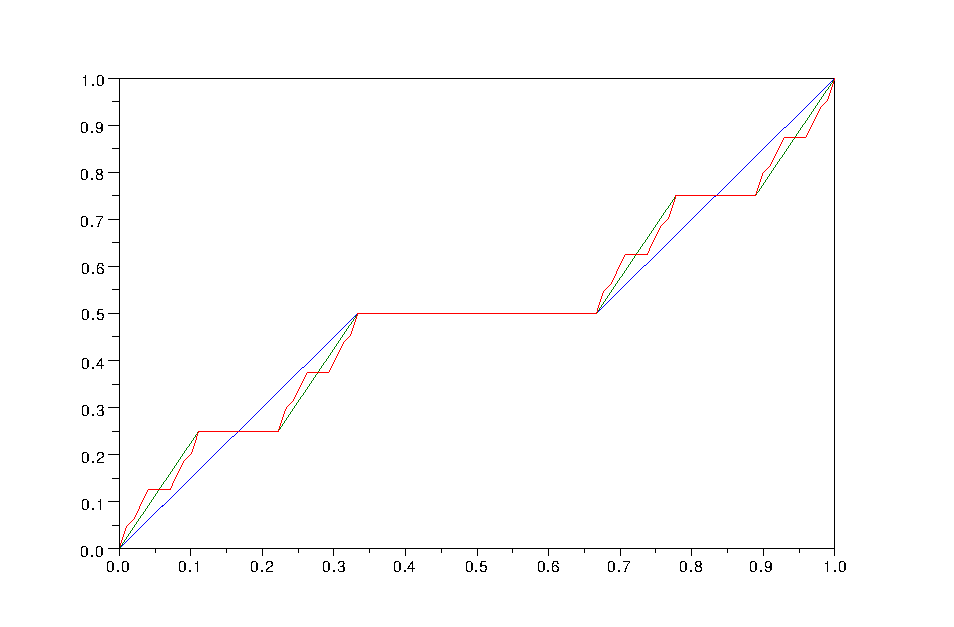
\includegraphics[scale=0.5]{images/cantor.pdf}
\caption{Fonction de Cantor}\label{ch6:fig1}
\end{center}
\end{figure}
$f$ sera
dérivable en tout point $x$ tel que dans son développement en base $3$, $x=\sum_{n \in \mathbb{N}}
a_i 3^{-i}$, il existe un $a_i$ de valeur $1$ et au moins un $a_j, j > i$ non
nul (on vérifiera que cette condition signifie que $x$ appartient à un
intervalle ouvert sur lequel l'une des fonctions $f_n$ est constante). Sur tous
ces points, la dérivée de $f$ est nulle. Le complémentaire de ces points est une
intersection dénombrable d'ensembles fermés (voir figure \ref{ch6:fig2}), donc
mesurable, et un calcul élémentaire de limite montre que sa mesure est nulle (vérifier sur la
figure \ref{ch6:fig2} que la mesure de $F_n$ est $\frac{2^n}{3^n}$). On en déduit que
$f^\prime$ existe pour presque tout $x$, mais aussi que pour tout $x \in [0,1]$:
\[
\int_{[0,x]} f^\prime(t) d \lambda(t) = 0 \neq f(x)
\]
\begin{figure}[hb]
\begin{center}
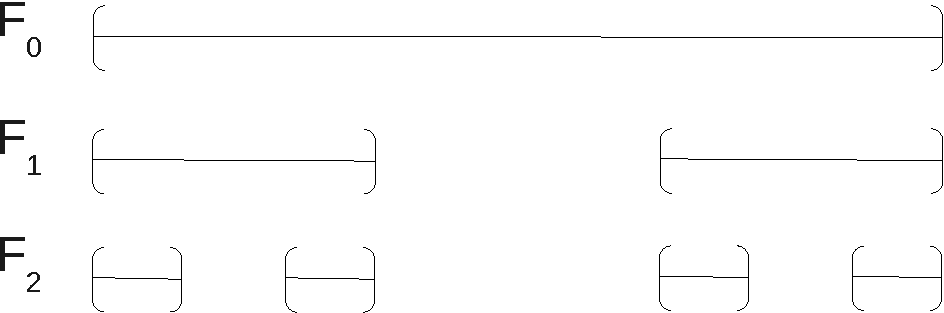
\includegraphics[scale=0.5]{images/ens_cantor.pdf}
\caption{Ensemble de Cantor}\label{ch6:fig2}
\end{center}
\end{figure}
La fonction de Cantor est un cas particulier d'une application singulière:
\begin{defn}
Une application $f$ définie sur $\mathbb{R}$ est dite singulière si elle est
dérivable en presque tout point et de dérivée nulle.
\end{defn}
Une application singulière ne peut pas être égale à l'intégrale de sa
dérivée.
\begin{defn}
Soit $F \colon [a,b] \to \mathbb{R}$. On dira que $F$ est absolument continue
pour tout $\epsilon > 0$ il existe un $\delta > 0$ telle que pour toute famille
finie d'intervalles $]a_i, b_i[, i = 1, \dots, n$:
\[
\sum_{i=1}^n (b_i - a_i) < \delta \Rightarrow \sum_{i=1}^n
\left(F(b_i)-F(a_i)\right) < \epsilon
\]
\end{defn}
\begin{mandatory}
\begin{theorem}{(Théorème fondamental de l'analyse)}
Soit $F$ une application absolument continue sur un intervalle $[a,b]$. Alors
$F$ est dérivable sauf sur un ensemble de mesure de Lebesgue nulle. Si
$f=F^\prime$ $\lambda$-presque partout, alors $f$ est sommable et pour tout $x
\in [a,b]$:
\[
F(x) = F(a) + \int_{[a,x]} f(t) d \lambda(t)
\]
\end{theorem}
\end{mandatory}
Ce théorème  repose sur le lemme de Vitali.
\begin{defn}
Soit $A$ une partie de $\mathbb{R}$. Un recouvrement de Vitali de $A$ est une
famille d'intervalles fermés $([a_i,b_i])_{i \in \mathbb{N}}$ telle que pour
tout $x \in A$ et pour tout $\epsilon > 0$ il existe un intervalle $[a_j,b_j]$
contenant $x$ tel que $b_j-a_j < \epsilon$.
\end{defn}
\begin{lemme}{(Lemme de Vitali)}
Soit $A$ une partie mesurable de $\mathbb{R}$ de mesure de Lebesgue finie. Soit
$\mathcal{V}$ un recouvrement de Vitali de $A$ par des intervalles de longueur
bornée par $M >0$. Pour tout $\epsilon > 0$, il existe une famille disjointe
finie $(I_i)_{i=1, \dots, n}$ d'intervalles de $\mathcal{V}$ telle que:
\[
\sum_{i=1}^n \lambda(I_i) \geq \lambda(A) - \epsilon
\]
\end{lemme}
\begin{proof}
On se fixe $\epsilon > 0$. 
Par définition de la mesure de Lebesgue, il existe un ouvert $U$ contenant $A$
et tel que $\lambda(U) \leq \lambda(A) + \epsilon$. Pour tout $x$ dans $A$, il
existe nécessairement un réel $\eta$ tel que tout intervalle de $\mathcal{V}$
soit contenu dans $U$ dès que sa longueur est inférieure à $\eta$. L'ensemble
des intervalle de $\mathcal{V}$ qui sont dans $U$ forme donc encore un
recouvrement de Vitali de $A$. On supposera donc dans la suite que $\mathcal{V}$
lui-même vérifie cette propriété.
 On pose:
\[
K =  \sup\{ b_i-a_i, \, [a_i,b_i]\in
\mathcal{V}\}
\]
 Soit $I_0 = [a_0,b_0]$ un intervalle de $\mathcal{V}$ tel que
$b_0 - a_0 \geq \frac{K}{2}$. On définit récursivement une suite $(I_n)_{n \in
\mathbb{N}}$ d'intervalles de $\mathcal{V}$ de la façon suivante.
$I_n=[a_n,b_n]$ est choisi disjoint de $\bigcup_{j=0}^{n-1} I_j$ et tel que:
\[
b_n - a_n \geq \frac{1}{2}\sup\left\{  b_i-a_i, \, [a_i,b_i]\in
\mathcal{V}, \, [a_i,b_i] \cap \bigcup_{j=0}^{n-1} I_j = \emptyset \right\}
\]
S'il n'est pas possible de trouver un tel $I_n$, la construction se termine et
on a:
\[
A \subset \bigcup_{j=0}^{n-1} I_j \subset U
\]
La preuve est alors terminée. 
Sinon, les intervalles $I_n$ étant disjoints et par additivité des mesures:
\[
\sum_{n=0}^{+\infty} (b_n-a_n) \leq \lambda(U) < +\infty
\]
Il existe donc un entier $N$ tel que:
\[
\sum_{n \geq N} (b_n-a_n) \leq \frac{\epsilon}{5}
\]
Soit $x \in A - \bigcup_{n \in \mathbb{N}} I_n$. Il existe un intervalle $I$ de
$\mathcal{V}$ tel que $x \in I$ et un plus petit entier $k$ tel que $I \cap I_k
\neq \emptyset$ (ceci en raison du fait que la longueur des intervalles $I_n$
tend vers 0 lorsque $n$ tend vers $+\infty$). Par construction la longueur de
$I$ doit être plus grande que le double de la longueur de $I_k$. On pose $5I_k$
l'intervalle de même point milieu que $I_k$ et de longueur 5 fois plus grande.
On a $I \subset 5I_k$, on déduit donc que si $x \notin \bigcup_{n=0}^N I_n$,
alors $x \in  \bigcup_{k=N+1}^{+\infty} 5I_n$ et donc:
\[
\lambda\left(A - \bigcup_{n=0}^N I_n \right) <  \epsilon
\]
\end{proof}
\begin{lemme}
Soit $f \colon [a,b] \to \mathbb{R}$ une application absolument continue et
singulière. Alors $f$ est constante.
\end{lemme}
\begin{proof}
Il est suffisant de prouver que $f(a)=f(b)$, le même raisonnement s'appliquant à
tout sous-intervalle de $[a,b]$.
Soit $X \subset [a,b]$ l'ensemble de mesure $b-a$ sur lequel $f$ est dérivable.
Soit $\epsilon > 0$. En tout point $x$ de $X$ il existe un intervalle $I_x =
[x, x+h_x]$ tel que pour tout $y \in I_x$:
\[
\frac{|f(y)-f(x)|}{h_x} < \epsilon
\] 
En complétant par tout les intervalles fermés de longueur inférieure, on forme
un recouvrement de Vitali $\mathcal{V}$ de $X$. 
Par ailleurs, $f$ étant supposée absolument continue, il existe un $\delta > 0$
associé à $\epsilon$. Le lemme de Vitali permet d'extraire une famille finie
disjointe d'intervalles de $\mathcal{V}$, que l'on notera $I_i = [x_i,
y_i], i=1\dots n$, et telle que:
\[
\sum_{i=1}^n (y_i - x_i) > (b-a) - \delta
\]
On pose $y_0 = a, x_{n+1}=b$. L'inégalité précédente donne:
\[
\sum_{i=0}^n (x_{i+1}-y_i) < \delta
\]
et par absolue continuité de $f$:
\[
\sum_{i=0}^n |f(x_{i+1}) - f(y_i)| < \epsilon
\]
D'autre part:
\[
\sum_{i=1}^n |f(y_i)-f(x_i)| < \epsilon \sum_{i=1}^n (y_i-x_i) \leq \epsilon
(b-a)
\]
soit finalement:
\[
|f(b)-f(a)| \leq \sum_{i=0}^n |f(x_{i+1}) - f(y_i)| + \sum_{i=1}^n
|f(y_i)-f(x_i)| \leq \epsilon (1 + b - a)
\]
d'où l'on tire $f(b)=f(a)$ en faisant $\epsilon \to 0$.
\end{proof}
On peut maintenir revenir à la preuve du théorème principal. On admettra la
première partie de la proposition qui est l'existence d'une dérivée $f^\prime$
en presque tout point et la sommabilité de $f^\prime$: dans l'utilisation
courante du théorème, qui concerne le calcul d'intégrale par primitives,
$f^\prime$ est connue et sommable. 
Pour ce qui concerne la second partie, on sait que l'application:
\[
h \colon x \in [a,b] \mapsto \int_{[a,x]} f^\prime(x) d \lambda(x)
\]
est dérivable, de dérivée presque partout égale $f^\prime$. L'application $f-h$ est donc singulière et
absolument continue, donc constante, ce qui prouve la seconde partie du théorème.
\section{Produit de convolution}
\begin{mandatory}
\begin{prop}
Soit $f,g$ deux applications de $L^1(\mathbb{R},
\mathcal{B}(\mathbb{R}), \lambda)$. 
\begin{itemize}
\item Pour presque tout $x$, l'application~:
\[
y \to f(x-y)g(y)
\]
est sommable.
\item L'application~:
\[
f * g = \left \{
\begin{array}{cc}
\int_{\mathbb{R}} f(x-y) g(y) d\lambda(y) & \mbox{ si } y \to f(x-y)g(y) \mbox{
sommable } \\
0 & \mbox{ sinon }
\end{array}
\right .
\]
est sommable et $\|f*g \|_1 \leq \|f\|_1 \|g\|_1$
\end{itemize}
\end{prop}
\end{mandatory}
\begin{proof}
L'application $y  \to x-y$ est continue, donc mesurable. L'application
$y \to f(x-y)$ est donc mesurable. Il en est de même de $(x,y) \to
f(x-y)$, composée de la projection canonique avec une application
mesurable. De même $(x,y) \to g(y)$ mesurable, donc $(x,y) \to
f(x-y)g(y)$ mesurable.
Par le théorème de Tonnelli et en utilisant l'invariance par
translation de la mesure de Lebesgue~:
\[
\int_{\mathbb{R}^2} |f(x-y)g(y)| d\lambda \times \lambda =
\int_{\mathbb{R}} \int_{\mathbb{R}} |f(x-y)g(y)| d \lambda(x) d
\lambda(y) = \|f\|_1 \|g\|_1
\]
On en déduit que $(x,y)\to f(x-y)g(y)$ est sommable. Le théorème de
Fubini s'applique alors et montre que $f*g$ est défini presque partout
et sommable. Comme~:
\[
\left | \int_{\mathbb{R}} f(x-y)g(y) d \lambda(y) \right | \leq  \int_{\mathbb{R}} |f(x-y)g(y)| d \lambda(y)
\]
on a~: $\|f*g \|_1 \leq \|f\|_1 \|g\|_1$.
\end{proof}
Le produit de convolution est une opération fondamentale du traitement
du signal qui correspond au filtrage linéaire stationnaire. Nous
verrons ultérieurement que le produit de convolution possède des
propriétés très intéressantes vis à vis de la transformation de Fourier.


% \chapter{Transformation de Fourier}
\section{Introduction}
La transformation de Fourier a été introduite en 1822 par J. Fourier au
cours de ses travaux sur l'équation de la chaleur. Son assertion initiale était
que toute application périodique pouvait se décomposer sous la forme d'une série
de fonctions sinus (ou cosinus), de fréquences multiples de l'inverse de la
période de l'application. Bien qu'inexacte en général, cette écriture a ouvert
la voie à une famille de représentation de fonctions éventuellement discontinues
sous la forme d'une série d'applications elles-même très régulières. En
interprétant les sommes de Fourier comme des sommes de Riemann, on peut
également étendre la théorie à une transformation intégrale, d'une grande
importance aussi bien pour les applications (traitement du signal en
particulier) que du point de vue fondamental (équations aux dérivées
partielles). La grande force de la transformation de Fourier est de permettre
une reformulation des opérateurs différentiels en opérateurs effectuant des
produits par des applications polynomiales: résoudre une équation différentielle
dans ce cadre revient à résoudre une équation ordinaire (que l'on espère plus
simple). 
\section{Transformée de Fourier des applications de $L^1$}
\begin{mandatory}
\begin{defn}
Soit $f : \mathbb{R}^n \to \mathbb{C}$ une application de
$L^1(\mathbb{R}^n)$. La transformée de Fourier de $f$ est
l'application $\widehat{f} : \mathbb{R}^n \to \mathbb{C}$ définie
par~:
\[
\forall \xi \in \mathbb{R}^n, \widehat{f}(\xi) = \int_{\mathbb{R}^n}
f(x) e^{-i \langle x ,\xi \rangle} d \lambda(x)
\]
\end{defn}
\end{mandatory}
\begin{rem}
Dans certains cas, on trouve une définition de la transformation de
Fourier faisant apparaître un facteur $2\pi$ devant le produit
scalaire~: ceci ne change rien aux propriétés fondamentales, sauf en
ce qui concerne la formule d'inversion que nous verrons plus loin. Cette
formulation alternative est la plus courant en traitement du signal, où l'on
recherche une interprétation de la variable de Fourier en terme de fréquence.
\end{rem}
On utilisera dans la suite indifféremment la notation $\widehat{f}$ ou
$\mathcal{F}(f)$ pour désigner la transformée de Fourier de $f$.
\begin{mandatory}
\begin{prop}
La transformée de fourier d'une application de $L^1(\mathbb{R}^n)$ est
une application de $L^\infty(\mathbb{R}^n)$. La transformation de
Fourier est un opérateur linéaire continu entre ces deux ensembles.
\end{prop}
\end{mandatory}
\begin{proof}
On a de façon évidente~:
\[
\forall \xi \in \mathbb{R}^n, \, |\widehat{f}(\xi)| \leq
\int_{\mathbb{R}^n} | f(x) | d\lambda(x)
\]
d'où~:
\[
\| \widehat{f} \|_{\infty} \leq \| f \|_1
\]
ce qui montre la continuité de l'opérateur linéaire défini par la
transformée de Fourier.
\end{proof}
\begin{exercice}
Déterminer les transformées de Fourier des applications suivantes~:
\[
\begin{array}{c}
f_1 \colon x \mapsto e^{-|x|} \\
f_2 \colon x \mapsto \begin{cases}
1-|x| & \text{ si } |x| \leq 1 \\
0 & \text{ sinon }
\end{cases}
\end{array}
\]
\end{exercice}
Le lemme suivant est important pour établir les formules d'inversion de la
transformation de Fourier:
\begin{mandatory}
\begin{prop}\label{fourier:1}
Soient $f,g \in L^1(\mathbb{R}^n)$. On a~:
\[
\int_{\mathbb{R}^n} f(x) \widehat{g}(x) d \lambda(x) = \int_{\mathbb{R}^n} \widehat{f}(y) g(y) d \lambda(y)
\]
\end{prop}
\end{mandatory}
\begin{proof}
Les applications $f, g$ étant dans $L^1(\mathbb{R}^n)$,
l'application $(x,y) \to f(x)g(y)$ est dans $L^1(\mathbb{R}^{2n})$. 
Pour prouver ce fait, on note tout d'abord que l'application $(x,y) \mapsto
f(x)$ est mesurable car composée de la projection sur le premier facteur et de
l'application $f$. De même pour l'application $(x,y) \mapsto g(y)$. On en déduit
que l'application: $(x,y) \mapsto f(x)g(y)$ est mesurable car produit
d'applications mesurables. Le théorème de Tonnelli permet alors d'écrire:
\[
\int_{\mathbb{R}^{2n}}|f(x)g(y)|d\lambda(x)d\lambda(y) = \int_{\mathbb{R}^n}
|f(x)| d \lambda(x)\int_{\mathbb{R}^n}
|g(y)| d \lambda(y) < +\infty
\]
 On en
déduit par application du théorème de Fubini~:
\begin{align*}
& \int_{\mathbb{R}^n} f(x) \int_{\mathbb{R}^n} g(y) e^{-i \langle x,y
      \rangle} d \lambda(y) d  \lambda(x) = \\
& \int_{\mathbb{R}^{2n}} f(x) g(y) e^{-i \langle x,y
      \rangle} d \lambda (x,y) = \\
&\int_{\mathbb{R}^n} g(y) \int_{\mathbb{R}^n} f(x) e^{-i \langle x,y
      \rangle} d \lambda(x) d  \lambda(y) 
\end{align*}
ce qui montre la proposition.
\end{proof}
La transformation de Fourier posséde un comportement simple vis à vis des
opérations de translation et de changement d'échelle. Le résultat ci-dessous est
donné sans démonstration, que le lecteur pourra faire à titre d'exercice.
\begin{mandatory}
\begin{prop}
Soit $f \in L^1(\mathbb{R}^n)$. Soit $v \in \mathbb{R}^n$. On définit la
translatée de $f$ en $v$ par:
\[
T_v f \colon x \in \mathbb{R}^n \mapsto f(x-v)
\]
On a alors:
\[
\forall \xi \in \mathbb{R}^n, \, \widehat{T_v f}(\xi) = e^{-i \langle
v, \xi \rangle}\widehat{f}(\xi)
\]
De même, soit $t > 0$ un réel. La dilatée de $f$ par $t$ est l'application:
\[
S_t f \colon x \in \mathbb{R}^n \mapsto t^{-n} f\left(\frac{x}{t}\right)
\]
On a:
\[
\forall \xi \in \mathbb{R}^n, \, \widehat{S_t f}(\xi) = \widehat{f}(t \xi)
\]
\end{prop}
\end{mandatory}
Enfin, comme annoncé en introduction, une dérivée partielle sera transformée en
multiplication par un monôme.
\begin{term}
On notera $D_jf$  la dérivée partielle de $f$ par rapport à la
$j$-ième coordonnée.
\end{term}
\begin{mandatory}
\begin{prop}
Soit $j \in \{ 1 \dots n \}$.
Soit $f \in L^1(\mathbb{R}^n)$ telle que l'application $x \to x_j
f(x)$ (avec $x_j$ $j$-ième composante du vecteur $x$) soit dans
$L^1(\mathbb{R}^n)$ alors~:
\[
D_j \widehat{f} = - i \widehat{x_j f(x)}
\]
\end{prop}
\end{mandatory}
\begin{proof}
La transformée de Fourier de $f$ est définie par~:
\[
\widehat{f}(\xi) = \int_{\mathbb{R}^n} f(x) e^{- i \langle x, \xi
  \rangle } d \lambda(x)
\]
Il s'agit d'une intégrale dépendant d'un paramètre. Comme par ailleurs
on a pour tout $x_0 \in \mathbb{R}^n$ et tout réel $h$~:
\[
|f(x) e^{-i \langle x, \xi  \rangle } - f(x) e^{-i \langle x, \xi + h
 e_j  \rangle }  |\leq |f(x)||x_j h|
\]
Le théorème de dérivation s'applique donc et donne le résultat.
\end{proof}
\begin{lemme}
L'ensemble des applications continues à support compact est dense dans
$L^1(\mathbb{R}^n)$. 
\end{lemme}
\begin{proof}
Les applications étagées sont denses de façon évidente dans
$L^1(\mathbb{R}^n)$. Montrons dans un premier temps que l'espace
engendré par les applications de la forme~:
\[
1_{\prod_{i=1\dots n} ]a_i, b_i[}
\]
est dense dans $L^1(\mathbb{R}^n)$. Soit $A$ un borélien borné.
Par définition de
la mesure de Lebesgue, il existe, pour tout $\epsilon >0$, une suite 
d'hyperrectangles $R_j = \prod_{i=1\dots n} ]a_i(j), b_i(j)[$ telle que $\cup_j R_j \supset A$ et~:
\[
\sum_j \lambda(R_j) < \lambda(A) + \frac{\epsilon}{2}
\]
par ailleurs, $A$ étant borné, la série $\sum_j \lambda(R_j)$ est
convergente. Il existe donc un entier $n_0$ tel que $\sum_{j > n_0}
\lambda(R_j) < \frac{\epsilon}{2}$. L'application~:
\[
g = \sum_{j=1}^{n_0} 1_{R_j} 
\]
vérifie alors $\| 1_A -g \|_1 < \epsilon$. 
Soit maintenant un hyperrectangle $R = \prod_{i=1\dots n} ]a_i, b_i[$
  et soit pour $\eta > 0$, l'application~:
\[
h_\eta : x \to \left  \{
\begin{array}{ll}
0 & x \notin [0,1] \\
\frac{x}{\eta} & 0 \leq x < \eta \\
1 & \eta \leq x < 1-\eta \\
\frac{1-x}{\eta} & 1-\eta \leq x \leq 1
\end{array}
\right .
\]
L'application~:
\[
g : x \to \prod_{i=1\dots n} h_\eta \left ( \frac{x_i - a_i +\eta}{b_i
  - a_i + 2 \eta} 
\right )
\]
est continue et~:
\[
\| 1_R - g \|_1 \leq \prod_{i=1\dots n} (b_i - a_i + 2 \eta) -
\prod_{i=1\dots n} (b_i - a_i) 
\]  
ce qui achève la démonstration, $\eta$ étant arbitraire.
\end{proof}
\begin{prop}\label{dens:1}
L'ensemble des applications indéfiniment dérivables à support compact
est dense dans $L^1(\mathbb{R}^n)$. 
\end{prop}
\begin{proof}
Il suffit de trouver une application indéfiniment dérivable vérifiant
les mêmes propriétés que $h$ dans la démonstration précédente. Il
existe tout d'abord des applications indéfiniment dérivables à support
compact. On peut par exemple prendre, sur $[0,1]$~:
\[
\psi : x \to \exp \left (
\frac{-1}{x(1-x)}
\right )
\]
Considérons maintenant~:
\[
\phi : x \to \left  \{
\begin{array}{ll}
0 & x < 0 \\
\int_{[0,x]} \psi d \lambda / \int_{[0,1]} \psi d \lambda & x \in ]0,
1[ \\
1 & x \geq 1
\end{array}
\right .
\]
L'application $\psi$ est indéfiniment dérivable. On est maintenant en
mesure d'exhiber une application semblable à $h$ de la démonstration
précédente, mais indéfiniment dérivable~:
\[
h_\eta : x \to \left  \{
\begin{array}{ll}
0 & x \notin [0,1] \\
\phi \left (\frac{x}{\eta} \right ) & 0 \geq x < \eta \\
1 & \eta \geq x < 1-\eta \\
\phi \left (\frac{1-x}{\eta} \right ) & 1-\eta \geq x \leq 1
\end{array}
\right .
\]
\end{proof}
\begin{mandatory}
\begin{theorem} (Riemann-Lebesgue)
Soit $f \in L^1(\mathbb{R}^n)$. On a~:
\[
\lim_{\| \xi \| \to \infty} |\widehat{f}(\xi)| = 0
\]
\end{theorem}
\end{mandatory}
\begin{proof}
Soit $\phi$ application indéfiniment dérivable à support compact. On
a~:
\[
(1+\| \xi \|^2) \widehat{\phi}(\xi) = \mathcal{F}\left(\phi + \sum_{i=1}^n
  D^2_i \phi \right)(\xi) \leq \| \phi + \sum_{i=1}^n
  D^2_i \phi \|_1
\]
Le résultat est immédiat dans ce cas. Pour $f \in L^1(\mathbb{R}^n)$
quelconque, on applique la densité des applications indéfiniment
dérivables à support compact pour montrer que pour tout $\epsilon > 0$
il existe $\phi$ indéfiniment dérivable à support compact vérifiant
$\| f - \phi \|_1 < \epsilon$. Comme par ailleurs~:
\[
\widehat{f}(\xi) \leq \| f- \phi \|_1 + \widehat{\phi}(\xi)
\]
on a le résultat général.
\end{proof}
\begin{mandatory}
\begin{prop}
Soit $f \in L^1(\mathbb{R}^n)$ admettant une dérivée partielle $D_j f$
elle-même dans $ L^1(\mathbb{R}^n)$. On a~:
\[
\widehat{D_j f}(\xi) =  i \xi_j \widehat{f}(\xi)
\]
avec $\xi_j$ $j$-ième composante du vecteur $\xi$.
\end{prop}
\end{mandatory}
\begin{proof}
Il suffit de montrer le théorème pour une application $f : \mathbb{R}
\to \mathbb{C}$.
On a~:
\[
\widehat{f^\prime}(\xi) = \int_{\mathbb{R}} f^\prime (x) e^{-i \langle \xi,
  x \rangle } d \lambda(x)
\]
Le théorème de convergence dominée permet d'écrire~:
\[
\lim_{k \to + \infty} \int_{[-k,k]} f^\prime (x) e^{-i \langle \xi,
  x \rangle} d \lambda(x) = \widehat{f\prime}(\xi)
\]
en faisant une intégration par parties, on obtient~:
\begin{align*}
& \int_{[-k,k]} f^\prime(x) e^{-i \langle \xi,
  x \rangle } d \lambda(x) = \\
&[f(x) e^{-i \langle
  x, \xi \rangle }]_{-k}^k +  \int_{[-k,k]} i \xi f(x) e^{-i \langle\xi,
  x \rangle } d \lambda(x)
\end{align*}
comme par ailleurs $f(x) = f(0) +\int_{[0,x]} f^\prime(u) du$, $f$
admet une limite en $+\infty, -\infty$.$f$ étant sommable, cette
limite est nulle et l'on déduit le résultat en faisant $k \to +\infty$.
\end{proof}
Il est possible dans certains cas d'inverser la transformation de Fourier pour
obtenir la fonction de départ (en fait de façon plus précise, un représentant
de la même classe d'équivalence dans $L^1(\mathbb{R}^n$). Les contraintes qui
sont imposées à l'application dont on souhaite inverser la transformée de
Fourier sont néanmoins assez fortes (égalité presque partout avec une
application continue). Pour énoncer et démontrer la formule d'inversion, deux
lemmes sont nécessaires.
\begin{lemme}\label{fourier:3}
Soit l'application $\phi \colon \mathbb{R} \to \mathbb{R}$ définie par~:
\[
\phi : x \to \frac{1}{\sqrt{2\pi}}e^{-\frac{x^2}{2}}
\]
on a~:
\[
\widehat{\phi} : \xi \to e^{- \frac{\xi^2}{2}}
\]
\end{lemme}
\begin{proof}
L'application $\phi$ appartient à $L^1(\mathbb{R})$ et vérifie l'équation
différentielle $\phi^\prime + x \phi = 0$. Il suffit de montrer que $\widehat{\phi}$ vérifie la même.
Le théorème de dérivation des intégrales dépendant d'un paramètre
s'appliquant de façon évidente ($\phi$ est à décroissance
exponentielle)~:
\[
\widehat{\phi}^\prime(\xi) = -i \int
\frac{1}{\sqrt{2\pi}}e^{-\frac{x^2}{2}} x e^{-i \xi x} dx
\]
Par ailleurs, $\lim_{|x| \to +\infty} \phi(x) = 0$, d'où par intégration
par parties~:
\[
\widehat{\phi}^\prime(\xi) = - \xi \widehat{\phi}
\]
on en déduit que $\widehat{\phi}$ est solution de l'équation différentielle:
$$\widehat{\phi}^\prime(\xi)+\xi \widehat{\phi}(\xi)=0$$
 et donc:
\[
\widehat{\phi}(\xi) = K e^{-\frac{\xi^2}{2}}
\]
La constante $K$ se détermine en remarquant que l'on doit avoir~:
\[
\widehat{\phi}(0) = \int \frac{1}{\sqrt{2\pi}}e^{-\frac{x^2}{2}} dx = 1
\]
\end{proof}
Dans la suite, on posera pour $a > 0$:
\[
\phi_a \colon x \in \mathbb{R} \mapsto \frac{1}{a}
\exp\left(-\frac{x^2}{2a^2}\right)
\]
\begin{lemme}\label{fourier:4}
Soit $f \in L^1(\mathbb{R})$. On a $\lim_{a \to 0^+} f *
\phi_a = f$ dans $L^1(\mathbb{R})$.
\end{lemme}
\begin{proof}
On suppose dans un premier temps que $f$ est continue à support compact.
On a, en utilisant la parité de $\phi_a$:
\begin{align*}
f * \phi_a(y) & = \int_{\mathbb{R}} f(x) \phi_a(y-x) d \lambda(x) \\
&= \frac{1}{\sqrt{2\pi}} \int_\mathbb{R} f(x) a^{-1}
\exp\left(-\frac{(x-y)^2}{2a^2}\right) d \lambda(x)
\end{align*}
En effectuant le changement de variable $u=(x-y)a^{-1}$, on en déduit:
\[
f * \phi_a(y) = \frac{1}{\sqrt{2\pi}} \int_{\mathbb{R}} f(au+y)
\exp\left(-\frac{u^2}{2}\right) d\lambda(u)
\]
$f$ continue à support compact est bornée en valeur absolue par une constante
$M$, on a donc pour tout $u \in \mathbb{R}$:
\[
\left|f(au+y)
\exp\left(-\frac{u^2}{2}\right)\right| \leq M \exp\left(-\frac{u^2}{2}\right)
\]
Le théorème de convergence dominée s'applique, et en utilisant la continuité de
$f$, on a finalement pour $a \to 0^+$:
\[
\lim_{a \to 0^+} f * \phi_a(y) = f(y)
\]
Soit maintenant $f\in L^1(\mathbb{R})$ quelconque. Il existe une suite
d'applications continues à support compact $(f_n)_{n \in \mathbb{N}}$ de limite
$f$ dans $L^1(\mathbb{R})$. On a:
\[
\|f*\phi_a - f_n*\phi_a\|_1 = \|(f-f-n)*\phi_a\|_1 \leq \|f-f_n\|_1\|\phi_a\|_1
= \|f-f_n\|_1
\]
En passant à la limite $a \to 0^+$, on en déduit:
\[
\|\lim_{a\to 0^+}f*\phi_a - f_n\|_1  \leq \|f-f_n\|_1
\]
Puis, en faisant $n \to +\infty$:
\[
\|\lim_{a\to 0^+}f*\phi_a - f\|_1 = 0
\]
qui donne le résultat annoncé
\end{proof}
Ce résultat est intéressant en soi: il montre l'existence d'une approximation de
l'unité dans $L^1(\mathbb{R})$ pour le produit de convolution. On peut
utiliser cette propriété pour adjoindre une unité $\delta$ à $L^1(\mathbb{R})$
(mais cette unité n'est pas elle-même une application de $L^1(\mathbb{R})$). 

La formule d'inversion permet de calculer une application dont la tansformée
de Fourier est connue. Bien que relativement restrictive, elle est fréquemment
utilisée en traitement du signal pour passer du spectre fréquentiel au signal
qui lui a donné naissance.
\begin{mandatory}
\begin{theorem}{(Formule d'inversion)}
Soit $f \in L^1(\mathbb{R}^n)$ telle que $\widehat{f} \in L^1(\mathbb{R}^n)$.
L'application:
\[
x \in \mathbb{R}^n \mapsto \frac{1}{(2\pi)^n} \int_{\mathbb{R}^n}
\widehat{f}(\xi)\exp\left(i \langle x, \xi \rangle\right) d \lambda(\xi)
\]
est égale presque partout à $f$.
\end{theorem}
\end{mandatory}
\begin{proof}
Pour simplifier la preuve, on se placera dans $L^1(\mathbb{R})$, l'extension au
cas multi-dimensionnel se faisant par application du théorème de Fubini.
Soit $f \in L^1(\mathbb{R})$ telle que $\widehat{f} \in L^1(\mathbb{R})$. Pour
tout $a>0$, la proposition \ref{fourier:1} et le lemme \ref{fourier:3}
permettent d'écrire:
\begin{align*}
& \int_{\mathbb{R}}f(x) \frac{1}{a}\exp\left(-\frac{(y-x)^2}{2a^2}\right) d
\lambda(x) = \\
& \frac{1}{\sqrt{2\pi}} \int_{\mathbb{R}}
\widehat{f}(\xi)\exp\left(i \langle x, \xi
\rangle\right)\exp\left(-\frac{a^2\xi^2}{2}\right) d \lambda(\xi)
\end{align*}
Le membre de gauche de l'égalité est $\sqrt{2\pi}f*\phi_a$. 
On a de plus:
\[
\forall \xi \in \mathbb{R}, \,
\left|\widehat{f}(\xi)\exp\left(i \langle x, \xi
\rangle\right)\exp\left(-\frac{a^2\xi^2}{2}\right)\right| \leq |\widehat{f}(\xi)|
\]
Le théorème de convergence dominée s'applique donc au membre de droite et on en
déduit:
\[
\lim_{a \to 0^+} f * \phi_a = \frac{1}{2 \pi}  \int_{\mathbb{R}}
\widehat{f}(\xi)\exp\left(i \langle x, \xi
\rangle\right) d \lambda(\xi)
\]
Le lemme \ref{fourier:4} donne la conclusion recherchée.
\end{proof}
\begin{rem}
La transformée de Fourier inverse, au même titre que la transformée directe, est
une application bornée continue. Une application de $L^1(\mathbb{R}^n)$ ne
pourra donc avoir une transformée de Fourier dans $L^1(\mathbb{R}^n)$
que si elle est égale presque partout à une application continue bornée. 
\end{rem}
La transformation de Fourier possède de bonnes propriétés vis-à-vis du produit
de convolution:
\begin{mandatory}
\begin{prop}
Soient $f,g \in L^1(\mathbb{R})$. On a:
$$\mathcal{F}(f*g)=\mathcal{F}(f).\mathcal{F}(g)$$
 De plus, si
$\widehat{f},\widehat{g}$ sont dans $L^1(\mathbb{R})$, on a:
$$\mathcal{F}^{-1}(\widehat{f}*\widehat{g})=2 \pi
\mathcal{F}^{-1}(\widehat{f}).\mathcal{F}^{-1}(\widehat{g})=2 \pi f . g$$
\end{prop}
\end{mandatory}
\begin{proof}
Par définition du produit de convolution:
\[
(f*g)(y) = \int_{\mathbb{R}} f(y-x)g(x) d\lambda(x)
\]
Sa transformée de Fourier est:
\[
\mathcal{F}(f*g) \colon \xi \mapsto \int_{\mathbb{R}} \left ( \int_{\mathbb{R}}
f(y-x)g(x) d\lambda(x) \right) e^{-i y \xi} d\lambda(y)
\]
L'application:
\[
(x,y) \in \mathbb{R}^2 \mapsto f(y-x)g(x)e^{-iy \xi}
\]
est sommable (cf démonstration dans la section sur le produit de convolution),
le théorème de Fubini et le changement de variable $u=y-x$ donnent:
\begin{align*}
\mathcal{F}(f*g)(\xi) & = \int_{\mathbb{R}^2}
f(y-x)g(x)   e^{-i (y-x) \xi}e^{-i x \xi} d\lambda(x)d\lambda(y) \\
& = \int_{\mathbb{R}^2}
f(u)g(x)   e^{-i u \xi}e^{-i x \xi} d\lambda(x)d\lambda(u) \\
& \int_{\mathbb{R}}
f(u)   e^{-i u \xi}d\lambda(u)  \int_{\mathbb{R}}g(x) e^{-i x \xi}
d\lambda(x) = \mathcal{F}(f)(\xi).\mathcal{F}(g)(\xi)
\end{align*}
La propostion relative à la transformée inverse est en tout point similaire, une
précaution étant néanmoins à prendre du fait de la présence du facteur $2\pi$.
\end{proof}
\section{Transformation de Fourier dans $L^2$}
La transformation de Fourier des applications de  $L^2(\mathbb{R}^n)$ ne peut pas se faire directement
à l'aide d'intégrales. Il faut procéder par extension en définissant
dans un premier temps cette transformation sur une classe plus
restreinte d'applications, stable par transformation de Fourier et dense dans 
$L^2(\mathbb{R}^n)$. Cette classe est celle des applications indéfiniment
dérivables à décroissance rapide que l'on va maintenant introduire, et sur
laqulle on montrera que la transformation de Fourier est un endomorphisme.
\begin{mandatory} 
\begin{defn}
Une application $f : \mathbb{R}^n \to \mathbb{C}$ est dite
indéfiniment dérivable à décroissance rapide si~:
\begin{itemize}
\item $f \in C^\infty(\mathbb{R}^n)$
\item $\forall (n,m) \in
\mathbb{N}^2, \, \lim_{|x|\to +\infty} \left |
x^n \frac{d^m f}{dx^m} \right | = 0$
\end{itemize}
\end{defn}
\end{mandatory}
\begin{term}
L'ensemble des applications indéfiniment dérivables à décroissance
rapide est appelé classe des applications de Schwartz et se note $\mathcal{S}( \mathbb{R}^n)$.
\end{term}

Il est clair que toute application de la classe $\mathcal{S}$ est
élément de $L^p(\mathbb{R}^n)$ pour tout $p \geq 1$. On définira la
transformée de Fourier d'une application de $\mathcal{S}$ par la
formule intégrale vue pour les applications sommables. 
\begin{mandatory}
\begin{prop}
Soit $f \in \mathcal{S}$. La transformée de Fourier de $f$ est encore
une application de $\mathcal{S}$.
\end{prop}
\end{mandatory}
\begin{proof}
Le caractère indéfiniment dérivable s'obtient aisément à partir du
théorème de dérivation sous le signe somme. Soit en effet un
multi-indice $I$ de longueur $p$. On écrit, pour tout $x$~:
\[
D_I e^{- i \langle x, \xi \rangle} = (-i)^n \left (\prod_{i \in I} x_i
\right )  e^{- i \langle x, \xi \rangle}
\]
Le terme $\prod_{i \in I} x_i$ se majore en valeur absolue par
$(1+\|x\|^2)^p$. Comme par ailleurs il est clair que les applications
$f(x)(1+\|x\|^2)^N$ sont sommables pour tout $N$, la dérivablité
d'ordre quelconque est obtenue.
En ce qui concerne la décroissance rapide, il suffit de reprendre la
démonstration du théorème de Riemann-Lebesgue en poursuivant les
intégrations par parties aussi loin que nécessaire (le caratère
$C^\infty$ des applications de $\mathcal{S}$ autorisant cette opération).
\end{proof}
Les applications de la classe $\mathcal{S}$ étant $L^1(\mathbb{R}^n)$, la
formule d'inversion précédemment établie est valable: la transformation de
Fourier est inversible en tant qu'opérateur linéaire continu $\mathcal{F}$ de
$\mathcal{S}$ dans lui-même et~:
\[
\mathcal{F}^{-1}(\widehat{f},x) = (2 \pi)^{-n} \int_{\mathbb{R}^n}
\widehat{f}(\xi) e^{i\langle \xi, y\rangle} d \lambda(\xi)
\]
\begin{mandatory}
\begin{prop}
Soit $f \in \mathcal{S}$ et $\widehat{f}$ sa transformée de
Fourier. On a~:
\[
 \int \|f\|^2 d \lambda = (2\pi)^{-n} \int \|\widehat{f}\|^2 d \lambda
\]
\end{prop}
\end{mandatory}
\begin{proof}
On vérifie immédiatement que pour tout $f \in \mathcal{S}$~:
\[
\overline{\mathcal{F}^{-1}(\widehat{f})} = \mathcal{F}(\overline{\widehat{f}})
\]
La proposition annoncée est alors un cas particulier de la proposition \ref{fourier:1}
\end{proof}
Cette dernière proposition montre que la transformation de fourier est
un endomorphisme quasi-isométrique de $\mathcal{S}$.
La définition de la transformation de Fourier des applications de
$L^2$ va se faire en utilisant la densité des applications
de $\mathcal{S}$ dans $L^2$ (voir proposition \ref{dens:1})
\begin{prop}
Soit $E$ un espace métrique et $A$ une partie dense de $E$. Soit $f
: A \to \mathbb{C}$ uniformément continue. Il existe une unique
extension continue de $f$ à $E$ que l'on continuera à noter $f$ par
abus de langage.
\end{prop}
\begin{proof}
Pour tout $x \in E$, il existe une suite $(x_n)$ d'éléments de $A$
avec $x = \lim_n x_n$. On définit l'extension par $f(x) = \lim_n
f(x_n)$. La suite $x_n$ étant convergente et $f$ continue, on vérifie
que la suite $f(x_n)$ est de Cauchy dans $\mathbb{C}$ complet, donc
admet une limite. Montrons que cette extension est continue en tout
point $x \in E$. Soit $\epsilon > 0$.  $f$ étant uniformément
continue, il existe  $\eta$ tel que~:
\[
\forall (u,v) \in A^2, d(u,v) < \eta
\Rightarrow |f(u)-f(v)| < \frac{\epsilon}{3}
\]
Par ailleurs, soit $(x_n)$ suite d'éléments de $A$ de limite $x$ et
$(y_n)$ de limite $y$. Il existe $n_0$ tel que pour tout $n \geq n_0$,
$d(x_n,x) < \frac{\eta}{3}$, $d(y_n,y) < \frac{\eta}{3}$ et
$|f(x_n)-f(x)| < \frac{\epsilon}{3}$, $|f(y_n)-f(y)| <
\frac{\epsilon}{3}$. On obtient alors $|f(x)-f(y)|< \epsilon$ pour
$d(x,y) < \frac{\eta}{3}$.
\end{proof}
\begin{mandatory}
\begin{defn}
La transformée de Fourier est l'unique extension à $L^2$ de
l'endomorphisme quasi-isométrique continu défini sur $\mathcal{S}$.
\end{defn}
\end{mandatory}
La transformation de Fourier ainsi définie est encore un endomorphisme
quasi-isométrique sur $L^2$ et pour tout $f \in L^2(\mathbb{R}^n)$:
\begin{mandatory}
\[
 \int \|f\|^2 d \lambda = (2\pi)^{-n} \int \|\widehat{f}\|^2 d \lambda
\]
\end{mandatory}
Les propriétés de la transformation de Fourier 
relativement aux translations, changements d'échelle et dérivations partielles
sont préservées dans $L^2(\mathbb{R}^n)$. Sous réserve du caractère $L^2$ des
produits, la proposition relative aux produits de convolution reste elle aussi
valable.
 Les définitions de la transformation de Fourier dans $L^1$ et dans
$L^2$ sont de formes très différentes. En revanche, il y a compatibilité au sens donné par la proposition suivante:
\begin{mandatory}
\begin{prop}
Soit $f \in L^1(\mathbb{R}^n) \cap L^2(\mathbb{R}^n)$. Alors
l'application:
\[
\widehat{f}(\xi) = \int_{\mathbb{R}^n} f(x) \exp \left(- i \langle x ,
\xi \rangle \right) d\lambda(x)
\]
est égale à la transformée de Fourier de $f$ dans $L^2(\mathbb{R}^n)$
\end{prop}
\end{mandatory}
\begin{proof}
Soit $f \in L^1(\mathbb{R}^n) \cap L^2(\mathbb{R}^n)$. On distinguera la
transformée de Fourier de $f$ dans $L^1(\mathbb{R}^n)$ de celle dans
$L^2(\mathbb{R}^n)$ en notant la première $\widehat{f}$ et la seconde
$\mathcal{F}(f)$, cette convention s'appliquant uniquement à la preuve courante.
Soit $\psi \in \mathcal{S}$ quelconque. La proposition \ref{fourier:1} donne:
\[
\int_{\mathbb{R}^n} \widehat{f}(\xi) \psi(\xi) d \lambda(\xi) =
\int_{\mathbb{R}^n} f(x) \widehat{\psi}(x) d \lambda(x)
\]
Soit $(\phi_n)_{n \in \mathbb{N}}$ une suite d'applications de $\mathcal{S}$
ayant pour limite $f$ dans $ L^2(\mathbb{R}^n)$. Par continuité du produit
scalaire (conséquence immédiate de l'inégalité de Cauchy-Schwartz):
\[
\lim_{n \to +\infty} \int_{\mathbb{R}^n} \phi_n(x) \widehat{\psi}(x) d
\lambda(x) = \int_{\mathbb{R}^n} f(x) \widehat{\psi}(x) d \lambda(x)
\]
La proposition \ref{fourier:1} donne:
\begin{align*}
& \lim_{n \to +\infty} \int_{\mathbb{R}^n} \phi_n(x) \widehat{\psi}(x) d
\lambda(x) = \\
  \lim_{n \to +\infty} \int_{\mathbb{R}^n} \widehat{\phi_n}(\xi)
  \psi(\xi) d \lambda(\xi) = \\
  & \int_{\mathbb{R}^n} \mathcal{F}(f)(\xi)
  \psi(\xi) d \lambda(\xi)
\end{align*}
On en déduit donc:
\[
\int_{\mathbb{R}^n} \left(\mathcal{F}(f)(\xi)-\widehat{f}(\xi)\right)
  \psi(\xi) d \lambda(\xi) = 0
\]
Puis par continuité du produit scalaire et densité de $\mathcal{S}$ dans 
$L^2(\mathbb{R}^n)$:
\[
\forall g \in  L^2(\mathbb{R}^n), \quad \int_{\mathbb{R}^n} \left(\mathcal{F}(f)(\xi)-\widehat{f}(\xi)\right)
  g(\xi) d \lambda(\xi) = 0
\]
prouvant ainsi que $\mathcal{F}(f)-\widehat{f}=0$ dans $L^2(\mathbb{R}^n)$.
\end{proof}

Le calcul pratique d'une transformation de Fourier dans $L^2(\mathbb{R}^n)$ est
parfois délicat: on ne peut généralement pas utiliser de forme intégrale, mais
uniquement des suites d'applications convergeant au sens $L^2$ vers
l'application cible. 
Une formule souvent utile est présentée dans l'exercice ci-dessous.
\begin{exercice}
Soit $f \in L^2(\mathbb{R})$. Soit $a > 0$. 
\begin{enumerate}
  \item Montrer que l'application $f_a = f 1_{[-a,a]}$ est sommable et que
  $\lim_{a \to +\infty}f_a=f$ dans $ L^2(\mathbb{R})$.
  \item En déduire que la transformée de Fourier de $f$ dans $L^2(\mathbb{R})$
  est la limite au sens $L^2$ pour $a \to +\infty$ de la famille d'applications:
  \[
  \xi \mapsto \int_{[-a,a]} f(x) \exp(-ix\xi) d\lambda(x)
  \]
\end{enumerate}
\end{exercice}
\begin{rem}
Cette formule n'apporte en soit rien de plus par rapport à la définition de la
transformée de Fourier utilisant les applications de la classe $\mathcal{S}$. En
revanche, si la limite:
\[
 \lim_{a \to +\infty} \int_{[-a,a]} f(x) \exp(-ix\xi) d\lambda(x)
\]
peut se calculer pour presque tout $\xi$, elle donne automatiquement un
représentant de la classe de la transformée de Fourier de $f$. Nous
verrons dans la suite du cours que des techniques utilisant des intégrales dans
le plan complexe permettent souvent de calculer des intégrales
généralisées de cette forme: beaucoup de transformations de Fourier sont
obtenues avec cette méthode.
\begin{exercice}
\begin{enumerate}
  \item Déterminer la transformation de Fourier inverse dans $L^2(\mathbb{R})$
  de l'application $1_{[-1,1]}$.
  \item En déduire la transformation de Fourier de l'application $\sinc$:
  \[
  x \in \mathbb{R} \mapsto \sinc(x) = \left\{
  \begin{array}{cc}
  	1 & \text{ si } x=0 \\
  	\frac{\sin x}{x} & \text{ si } x \neq 0 
  \end{array}
  \right.
  \]
  \item Pouvez-vous en déduire que $\sinc \notin L^1(\mathbb{R})$ ?
\end{enumerate}
\end{exercice}
Le caractère quasi-isométrique de la transformée de Fourier est parfois utile
pour calculer des intégrales lorsque la fonction à intégrer est le carré d'une
application $L^2$:
\begin{exercice}
Soit l'application~:
\[
f : x \to \left \{
\begin{array}{ll}
\frac{\sin^2 x }{x^2} & x \neq 0 \\
1 & x = 0
\end{array}
\right .
\]
\begin{itemize}
\item Montrer que $f \in L^1(\mathbb{R})$ et calculer $\widehat{f}$
(on pourra utiliser la transformation inverse de Fourier dans
$L^2(\mathbb{R})$ de l'application $\pi 1_{[-1,+1]}$ vue dans l'exercice
précédent et le produit de convolution).
\item En déduire la valeur des l'intégrales~:
\[
\int_{\mathbb{R}} \frac{\sin^2 x}{x^2} d \lambda(x)
\]
et
\[
\int_{\mathbb{R}} \frac{\sin^4 x}{x^4} d \lambda(x)
\]
\end{itemize}
\end{exercice}
\end{rem}

\chapter{Intégration des formes différentielles}
\section{Chemins}
Dans cette partie, on travaillera dans le cadre des ouverts de $\R^n$, qui sera dans la suite restreint à $\C$. 
\begin{fdefn}
Soit $U$ un ouvert de $\R^n$. Un chemin de classe $C^k$ par morceaux dans $U$ est une application continue $\gamma$ d'un intervalle réel $[a,b]$ dans $U$ telle qu'il existe une subdivision $a=t_0 < t_1 < \dots < t_N = b$ pour laquelle $\gamma$ est de classe $C^k$ sur chaque intervalle $]t_i,t_{i+1}[, \, i=0 \dots N$.
\end{fdefn}
Le point $\gamma(b)$ (resp. $\gamma(a)$) est appelé extrémité (resp. origine) du chemin.
Dans toute la suite, le terme "chemin" désignera de façon implicite un chemin de classe $C^k$ par morceaux, l'indice de régularité $k$ étant précisé lorsque cela est nécessaire. 
\begin{fdefn}
Soit $\gamma \colon [a,b] \to U$ un chemin. Soit $\phi \colon [c,d] \to [a,b]$ un difféomorphisme de classe $C^k$. Le chemin $\gamma \circ \phi$ sera dit obtenu à partir de $\gamma$ par changement de paramètre. Un changement de paramètre $\phi$ strictement croissant sera dit préserver l'orientation.
\end{fdefn}
Un chemin obtenu par changement de paramètre est géométriquement semblable au chemin initial. Son sens de parcours n'est pas modifié si le changement de paramètre préserve l'orientation. Dans toute la suite, les grandeurs associées aux chemins seront invariantes par changement de paramètre préservant l'orientation: on pourra donc choisir de façon arbitraire l'intervalle de définition d'un chemin de telle sorte que les calculs soient les plus simples possible. Pour les définitions qui vont suivre, on se placera sur l'intervalle $[0,1]$ afin d'alléger les écritures. 

\begin{fdefn}
Soient $\gamma_1, \gamma_2$ deux chemins de $[0,1]$ dans un ouvert $U$ de $\R^n$ tels que $\gamma_1(1) =
\gamma_2(0)$. Le chemin $\gamma_2 * \gamma_1$, composé de $\gamma_1$ et
$\gamma_2$, est défini par:
\[
\forall t \in [0,1], \, (\gamma_2 * \gamma_1)(t) = \left \{
\begin{array}{cc}
\gamma_1(2t) & \text{ si } t \in \left[0,\frac{1}{2}\right] \\
\gamma_2(2t-1) & \text{ si } t \in \left]\frac{1}{2},1\right]
\end{array}
\right.
\]
\end{fdefn}



\begin{fdefn}
Soit $\gamma$ un chemin de $[0,1]$ dans un ouvert $U$ de $\R^n$. Le chemin opposé, noté
$\gamma^-$, est défini par:
\[
\forall t \in [0,1], \, \gamma^-(t) = \gamma(1-t)
\]
\end{fdefn}
Le changement de paramètre $t \to 1-t$ ne préserve par l'orientation. 
Le chemin opposé possède la même image, mais un sens de parcours différent: on
démarre de l’extrémité du chemin original pour arriver à son origine. 
Les opérations sur les chemins sont résumées figure \ref{ch8:fig1}.
\begin{figure}[ht]
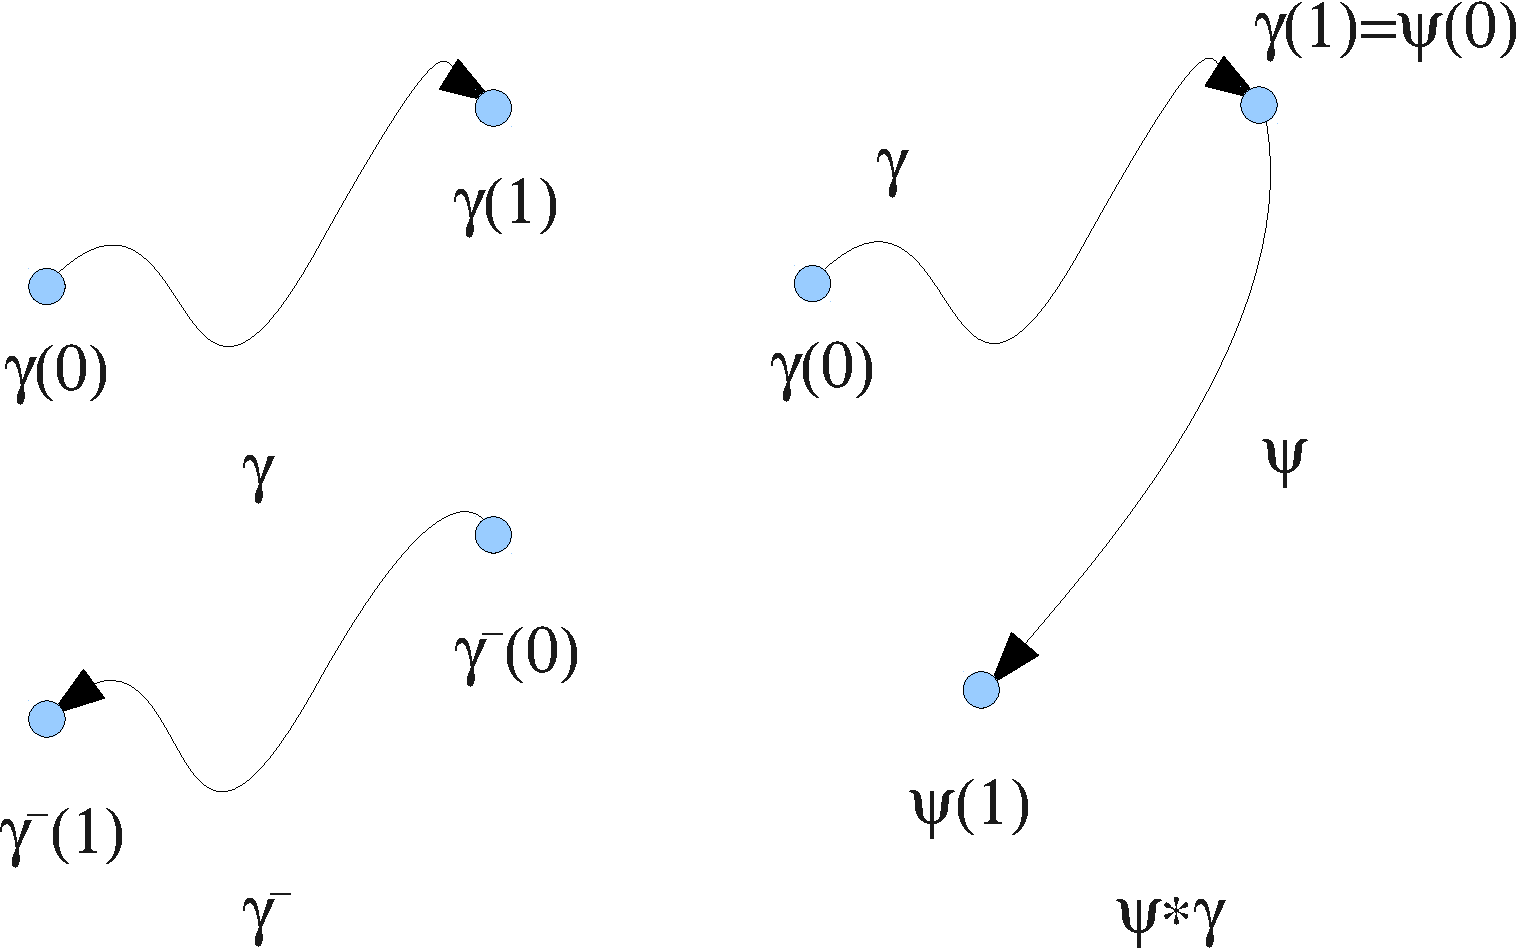
\includegraphics[scale=0.4]{images/chemins.pdf}
\caption{Chemins composé et inverse}\label{ch8:fig1}
\end{figure}

\begin{fdefn}
Un lacet $\gamma$ de $[0,1]$ dans $U$ ouvert de $\R^n$ est dit simple si, pour tout couple de points $(t_1,t_2) \in ]0,1[^2$, on a
$\gamma(t_1) \neq \gamma(t_2)$
\end{fdefn}

Il est possible de définir la longueur d'un chemin en l'approchant par des chemins polygonaux: c'est Archimède qui semble-t-il est le premier à avoir eu cette idée. La proposition suivante résume ce procédé.
\begin{fprop}
Soit $\gamma \colon [a,b] \to \R^n$ un chemin de classe $C^k$, $k \geq 1$. Pour toute subdivision $S = (a=t_0 < t_1 \dots < t_n = b)$ de l'intervalle $[a,b]$, on pose:
\[
l(S) = \sum_{i=0}^{n-1} \| \gamma(t_{i+1}) - \gamma(t_i) \|
\]
La borne supérieure de l'ensemble $\{l(S)\}$ où $S$ parcourt les subdivisions de $[a,b]$ est finie et vaut:
\[
l = \int_a^b \|\gamma^\prime(t)\| dt
\]
la valeur $l$ est appelée longueur du chemin $\gamma$.
\end{fprop}
\begin{proof}
On remarque tout d'abord, en vertu du théorème des accroissements finis que:
\[
\| \gamma(t_{i+1}) - \gamma(t_i) \|  = \left\| \int_{t_i}^{t_{i+1}} \gamma^\prime(s) ds \right\| \leq \int_{t_i}^{t_{i+1}}\left\| \gamma^\prime(s) \right\|ds
\]
on en déduit que pour toute subdivision $S$:
\[
l(S) \leq  \int_a^b \left\| \gamma^\prime(s) \right\|ds
\]
La borne supérieure de l'ensemble $l(S)$ où $S$ parcourt les subdivisions de $[a,b]$ est donc finie. Soit maintenant $\epsilon > 0$. l'application $\gamma$ étant de classe $C^1$, sa dérivée est continue sur le compact $[a,b]$, donc uniformément continue. On en déduit l'existence d'une valeur $\eta$ telle que pour toute subdivision $S =  (a=t_0 < t_1 \dots < t_n = b)$ vérifiant $\sup_{i=0}^{n-1}(t_{i+1}-t_i) < \eta$ on ait:
\[
\| \gamma^\prime(s) - \gamma^\prime(t_i)\| < \epsilon, s \in [t_i, t_{i+1}], i=0 \dots n-1
\]
Ceci implique que pour tout $i=0,\dots,n-1$:
\begin{align*}
\|\int_{t_i}^{t_{i+1}} \gamma^\prime(s) - \gamma^\prime(t_i) ds\| & = \| \gamma(t_{i+1}) - \gamma(t_i) - \gamma^\prime(t) (t_{i+1}- t_i) \| \\& < \epsilon (t_{i+1}-t_i)
\end{align*}
Soit finalement:
\[
\left| \|\gamma(t_{i+1}) - \gamma(t_i)\| -  \|\gamma^\prime(t) \|(t_{i+1}-t_i)\right | < \epsilon (t_{i+1}-t_i)
\]
On en déduit par sommation sur $i$ et application de l'inégalité triangulaire:
\[
\left|l(S) - \sum_{i=0}^n  \|\gamma^\prime(t) \|(t_{i+1}-t_i)\right| < \epsilon (b-a) 
\]
En réduisant éventuellement le pas $sup_{i=0}^{n-1}(t_{i+1}-t_i)$ des subdivisions considérées, on aura également:
\[
\left | \int_a^b \|\gamma^\prime(s)\| ds -  \sum_{i=0}^n  \|\gamma^\prime(t) \|(t_{i+1}-t_i)\right| < \epsilon (b-a) 
\]
ce qui termine la preuve. 
\end{proof}
Lorsque le chemin est de classe $C^k$ par morceaux, on définit sa longueur par sommation. 
\begin{fdefn}
Soit $\gamma \colon [a,b] \to \R^n$ un chemin de classe $C^k$ par morceaux qui est de classe $C^k$ sur chacun des intervalles $]t_i,t_{i+1}[$, où $(a=t_0 < t_1 \dots < t_n = b)$ est une subdivision de l'intervalle $[a,b]$. Sa longueur est définie par:
\[
\sum_{i=0}^{n-1} \int_{t_i}^{t_{i+1}} \| \gamma^\prime(t) \| dt
\]
\end{fdefn}
On peut montrer facilement que la longueur d'un chemin de classe $C^k$ par morceaux est encore la limite supérieure des approximations polygonales. La proposition suivante établit le fait que la longueur est un invariant géométrique d'un chemin. Elle se montre immédiatement en utilisant la formule du changement de variable dans les intégrales. 
\begin{fprop}
La longueur d'un chemin de classe $C^k$ par morceaux est invariante par changement de paramétrage.
\end{fprop}
\begin{rem}
Le procédé d'approximation par des chemins polygonaux permet de définir la longueur de chemins simplement continus, mais celle-ci peut être infinie. Lorsque la longueur est finie, on dit que le chemin est rectifiable. L'absence de formule de calcul utilisable dans le cas général fait qu'en pratique, on se restreint aux chemins de classe $C^k$ par morceaux. 
\end{rem}
\section{Intégration des formes différentielles}
\subsection{Un exemple introductif: le travail d'une force}
Le travail d'une force est en mécanique du point une notion fondamentale qui
permet de relier la variation d'énergie cinétique à l'intégrale d'une quantité
simple. Supposons donné un point matériel de masse $m$, se déplaçant dans
$\mathbb{R}^2$ et soumis à un champ de force $F \colon \mathbb{R}^2 \to
\mathbb{R}^2$ présent dans tout l'espace. En notant $\gamma \colon [a,b] \to
\mathbb{R}^2$ la trajectoire du point de l'instant $a$ à l'instant $b$, le principe fondamental
de la dynamique donne:
\[
\forall t \in ]a,b[, \, m \ddot{\gamma}(t) = F\left(\gamma(t)\right)
\]
Il est possible d'obtenir une intégrale première de cette relation en prenant le
produit scalaire avec la vitesse $\dot{\gamma}(t)$ des deux côtés de
l'égalité:
\[
\forall t \in ]a,b[, \, m \langle\ddot{\gamma}(t),\dot{\gamma}(t)\rangle =
\langle F\left(\gamma(t)\right), \dot{\gamma}(t) \rangle
\]
Comme:
\[
\frac{d\|\dot{\gamma}(t)\|^2}{dt}(t) = 2
\langle\ddot{\gamma}(t),\dot{\gamma}(t)\rangle
\]
on a, par intégration des deux membres et en supposant que la vitesse est
définie en $a$ et $b$:
\begin{equation}\label{eq:travail_force}
\frac{1}{2}m \|\dot{\gamma}(b)\|^2 - \frac{1}{2}m \|\dot{\gamma}(a)\|^2 =
\int_{[a,b]} \langle F\left(\gamma(t)\right), \dot{\gamma}(t) \rangle
dt
\end{equation}
On reconnaît en partie gauche la variation d'énergie cinétique entre $\gamma(a)$
et $\gamma(b)$, la partie droite étant le travail de la force $F$ le long du
chemin.
En règle générale, le travail dépend du chemin $\gamma$. Néanmoins, dans
certains cas, on peut montrer qu'il n'en est rien. En mécanique, ceci se produit
lorsque le champ de force dérive d'un potentiel, i.e. il existe une application
$\Psi \colon \mathbb{R}^2 \to \mathbb{R}$ telle que $F = \nabla \Psi$. On
rappelle que la notation $\nabla \Psi$ désigne le gradient de $\Psi$ qui est
défini par la relation:
\[
\forall x \in \mathbb{R}^2, \forall v \in \mathbb{R}^2, \, \langle \nabla
\Psi(x),v \rangle = \Psi^\prime(x)(v)
\]
Si l'on suppose que $F$ dérive d'un potentiel $\Psi$, le travail de $F$ s'écrit:
\begin{align*}
\int_{[a,b]} \langle F\left(\gamma(t)\right), \dot{\gamma}(t) \rangle
dt&  = \int_{[a,b]} \langle \nabla \Psi(\gamma(t)), \dot{\gamma}(t)
\rangle dt \\
&= \int_{[a,b]} \Psi^\prime(\gamma(t))(\dot{\gamma}(t)) dt \\
& = \int_{[a,b]} \frac{d}{dt}(\Psi\circ \gamma)(t) dt \\
& = \Psi\left(\gamma(b)\right) - \Psi\left(\gamma(a)\right)
\end{align*}
Cette dernière expression ne dépend plus que des points de départ et d'arrivée
et non de $\gamma$. 

L'expression de la variation de l'énergie cinétique \ref{eq:travail_force} est un exemple d'intégration d'une forme différentielle le long d'un chemin. On remarquera que la quantité $\langle F\left(\gamma(t)\right), \dot{\gamma}(t) \rangle$ exprime une projection tangentielle de $F\left(\gamma(t)\right)$ sur la courbe $\gamma$. 
\subsection{Formes différentielles}
\begin{fdefn}
Soit $U$ un ouvert de $\R^n$. On appelle forme différentielle de degré 1 et de régularité $k$ une application $\omega$ de classe $C^k$ de $U$ dans l'espace vectoriel des formes linéaires sur $\R^n$.  
\end{fdefn}
Pour un $x \in U$ fixé, $\omega(x)$ est une forme linéaire sur $\R^n$ et peut donc être appliquée à un vecteur $v \in \R^n$ pour donner un réel. On notera $\omega(x;v)$ le résultat de cette opération.

La quantité $\langle F\left(\gamma(t)\right), \dot{\gamma}(t) \rangle$ de l'exemple introductif se traduit facilement en terme de formes différentielles: il s'agit de $\omega(\gamma(t);\gamma^\prime(t))$ avec $\omega = \sum_{i=1}^2 F_i dx_i$

L'espace des formes linéaires sur $\R^n$ est canoniquement isomorphe à $\R^n$. On peut en effet prendre comme base les formes élémentaires $dx_i, i=1 \dots n$ qui à tout vecteur $v=(v_1,\dots,v_n)$ de $\R^n$ associent la $i$-ième coordonnée: $dx_i(v) = v_i$. Avec cette notation une forme différentielle $\omega$ de régularité $k$ pourra s'écrire $\omega = \sum_{i=1}^n \omega_i dx_i$ où les $\omega_i$ sont des fonctions de classe $C^k$ de $U$ dans $\R$. 
\begin{exercice}
Soit $f$ une application de classe $C^k$ définie d'un ouvert $U$ de $\R^n$ dans $\R$. Montrer que l'expression:
\[
df = \sum_{i=1}^n \frac{\partial f}{\partial x_i} dx_i
\]
définit une forme différentielle de degré 1 dont on précisera la régularité.
\end{exercice}
\begin{fdefn}
Soit $U$ un ouvert de $\R^n$. On appelle champ de vecteurs de classe $C^k$ sur $U$ une application de classe $C^k$ de $U$ dans $\R^n$. 
\end{fdefn}
De même que pour les formes différentielles, on peut écrire un champ de vecteurs en coordonnées $X(x) = (X_1(x),\dots X_n(x))$ avec $X_i, i=1 \dots n$ applications de classe $C^k$ de $U$ dans $\R$. 

Une forme différentielle de degré 1 $\omega = \sum_{i=1}^n \omega_i dx_i$ agit sur un champ de vecteurs $X$ selon la formule:
\[
x \in U \mapsto \omega(x;X(x)) = \sum_{i=1}^n \omega_i(x) X_i(x)
\]
On définit ainsi une application de $U$ dans $\R$ appelée produit contracté de $\omega$ et de $X$ et notée $(\omega | X)$. 
\begin{fdefn}
Soit $U$ ouvert de $\R^m$ et $V$ ouvert de $\R^n$. Soit $\phi \colon U \to V$ une application de classe $C^{k+1}$. A toute forme différentielle $\omega$ sur $V$ de régularité $k$ on associe une forme $\phi^*\omega$ de régularité $k$  sur $U$ définie pour tout $x$ dans $U$ et tout vecteur $v$ de $\R^m$ par la formule:
\[
\phi^*\omega(x,v) = \omega(\phi(x),\phi^\prime(x).v)
\]
La forme $\phi^*\omega$ est appelée image réciproque de $\omega$ par $\phi$.
\end{fdefn}
\begin{exercice}
En posant $\omega = \sum_{i=1}^n \omega_i dx_i$,
montrer que la forme $\phi^*\omega$ s'exprime sous la forme:
\[
\phi^*\omega = \sum_{j=1}^m \theta_j dx_j
\]
avec:
\[
\theta(x) = \phi^{\prime t} (x) \omega(\phi(x)) 
\]
où $\theta(x)$ (resp. $\omega(x)$) est le vecteur de composantes $\theta_j(x)$ (resp. $\omega_i(x)$) et $\phi^\prime(x)$ est la matrice de l'application dérivée de $\phi$ en $x$. 
\end{exercice}
L'image réciproque d'une forme différentielle s'apparente à un changement de variable. On peut procéder de même pour les champs de vecteurs, mais il s'agira ici d'une image directe.
\begin{fdefn}
Soit $U,V$ ouverts de $\R^n$. Soit $\phi \colon V \to U$ un difféomorphisme de classe $C^{k+1}$. A tout champ de vecteurs $X$ de classe $C^k$ défini sur $V$ on associe un champ de vecteurs $\phi_* X$ de classe $C^k$ sur $U$ par la formule:
\[
\phi_* X(x) = \phi^\prime(y) X(y)
\]
avec $y = \phi^{-1}(x)$.
\end{fdefn}
Contrairement à l'image réciproque d'une forme différentielle, l'image directe d'un champ de vecteurs n'est définie que pour des difféomorphismes. La proposition suivante découle directement des définitions et montre que les images directes et réciproques sont d'une certaine façon des opérations adjointes.  
\begin{prop}
Soit $U,V$ ouverts de $\R^n$. Soit $\phi \colon V \to U$ un difféomorphisme de classe $C^{k+1}$. Pour toute forme différentielle de degré 1 et de régularité $k$ sur $U$ et tout champ de vecteur de classe $C^k$ sur $V$ on a:
\[
\left(\phi^* \omega | X \right) = \left(\omega | \phi_* X \right)
\]
\end{prop}
On peut étendre la notion de forme différentielle à des degrés plus élevés:
\begin{fdefn}
Soit $U$ un ouvert de $\R^n$. On appelle forme différentielle de degré p et de régularité $k$ sur $U$ une application $\omega$ de classe $C^k$ de $U$ dans l'espace vectoriel $\Lambda^p_n$ des formes $p$-linéaires alternées sur $\R^n$. L'action au point $x$ d'une forme $\omega$ de degré $p$ sur les vecteurs $(v_1, \dots, v_p)$ sera notée $\omega(x;v_1,\dots,v_p)$. Une forme de degré 0 et de régularité $k$ sur $U$ est une application de classe $C^k$ sur $U$ à valeurs dans $\R$. 
\end{fdefn}
\begin{notation}
L'ensemble des formes différentielles de degré $p$ et de régularité $k$ sur un ouvert $U$ de $\R^n$ sera noté $\Omega_k^p(U)$.
\end{notation}
Contrairement au cas particulier $p=1$, une contrainte supplémentaire est exigée: le caractère alterné des formes linéaires. La raison de ce choix apparaîtra dans la suite lorsque on voudra interpréter une intégrale de forme comme une intégrale ordinaire.
Toute forme $p$-linéaire alternée sur $\R^n$ avec $p > n$ est identiquement nulle, on ne considérera donc que des formes de degré au plus $n$. L'espace vectoriel des formes $p$-linéaires alternées sur $\R^n$ est de dimension $C_n^p$. En effet, par la propriété de $p$-linéarité, il est suffisant de considérer l'action sur les $p$-uplets de vecteurs de base $(e_{i_1},\dots e_{i_p})$ où les indices $i_1,\dots i_p$ sont dans l'ensemble $\{1, \dots n\}$. Le caractère alterné permet de se restreindre encore aux seuls $p$-uplets $(e_{i_1},\dots e_{i_p})$ formés d'indices distincts rangés en ordre croissant, i.e. tels que $i_1 < i_2 < \dots < i_p$. On définit alors les formes $p$-alternées de base sur de tels $p$-uplets par:
\[
dx^{i_1\dots i_p}(e_{j_1},\dots,e_{j_p}) = \begin{cases}
1 \text{ si } i_1=j_1,\dots i_p=j_p \\
0 \text{ sinon }
\end{cases}
\]
\begin{fprop}
Soit $(v_1,\dots,v_p)$ un $p$-uplets de vecteurs de $\R^n$. On a:
\[
dx^{i_1\dots i_p}(v_1,\dots,v_p) = det(M) 
\]
où $M$ est la matrice $p \times p$ dont les lignes sont formées des coordonnées d'indice $i_1, \dots, i_p$ des vecteurs $v_1,\dots v_p$.
\end{fprop}
\begin{proof}
Par la $p$ linéarité et en notant $v_{jk}$ la coordonnée $k$ du vecteur $j$:
\[
dx^{i_1\dots i_p}(v_1,\dots,v_p) = \sum_{(k_1,\dots,k_p)} \prod_{j=1}^p v_{jk_j}dx^{i_1\dots i_p}(e_{k_1},\dots,e_{k_p})
\]
La définition des formes de base $dx^{i_1\dots i_p}$ montre que seuls les termes correspondant à des indices appartenant à l'ensemble $I = \{i_1, \dots , i_p\}$ sont non nuls. Il vient donc:
\[
dx^{i_1\dots i_p}(v_1,\dots,v_p) = \sum_{(k_1\in I,\dots,k_p\in I)} \prod_{j=1}^p v_{jk_j}dx^{i_1\dots i_p}(e_{k_1},\dots,e_{k_p})
\]
En utilisant le caractère alterné des formes, on peut se ramener par changement de signe au seul cas où les indices sont rangés en ordre croissant, qui donne une valeur de $1$ pour la forme de base. On en déduit l'expression:
\[
dx^{i_1\dots i_p}(v_1,\dots,v_p) = \sum_{\sigma \in \Sigma(I)} \epsilon(\sigma) \prod_{j=1}^p v_{j\sigma(i_j)}
\]
où $\Sigma(I)$ désigne l'ensemble des permutations de $I$ et $\epsilon(\sigma)$ la signature de la permutation $\sigma$. On remarque alors que cette expression est celle donnant le déterminant de la matrice $M$. 
\end{proof}
\begin{fdefn}
Un $p$-uplet d'indices $I=(i_1, \dots, i_p)$ est appelé multi-indice de longueur $p$. Il est dit ordonné si $i_1 < \dots < i_p$. La longueur d'un multi-indice $I$ est notée $|I|$.
\end{fdefn}
\begin{notation}
 Soit $I=(i_1, \dots, i_p)$ un multi-indice ordonné. On notera $dx^I$ la forme de base $dx^{i_1,\dots,i_p}$.
\end{notation}

Il est possible de définir un produit entre les formes différentielles, que l'on notera $\wedge$. 
Pour ce faire, on supposera donnés  deux multi-indices ordonnés disjoints $I=(i_1, \dots , i_p)$ et $J=(j_1, \dots j_q)$. Soit $K$ le multi-indice ordonné  $(k_1,\dots,k_{p+1})$ obtenu à partir des éléments de l'ensemble $I\cup J = \{i_1,\dots,i_p,j_1,\dots,j_q\}$. 
Il existe une unique permutation $\sigma$ associant à $(i_1,\dots,i_p,j_1,\dots,j_q)$ le multi-indice $K$. On pose:
\[
dx^I \wedge dx^J = \epsilon(\sigma) dx^K
\]
Si les deux multi-indices ordonnés $I,J$ ne sont pas disjoints, on posera $dx^I \wedge dx^J = 0$.
Un produit étant une application bilinéaire, $\wedge$ est défini de façon unique pour des formes quelconques à partir de la relation précédente. L'opération $\wedge$ est appelée produit extérieur. 
\begin{fprop}
Soient $\omega,\theta,\rho$ trois formes multilinéaires alternées de degrés respectifs $p,q,r$. On a:
\begin{enumerate}
\item $\omega \wedge \theta = (-1)^{pq} \theta \wedge \omega$.
\item $(\omega \wedge \theta) \wedge \rho = \omega \wedge (\theta \wedge \rho)$.
\item $\omega \wedge \omega = 0$.
\end{enumerate}
\end{fprop}
\begin{proof}
Il suffit de vérifier ces propriétés sur les formes de base $dx^I$, sur lesquelles elles sont immédiates.
\end{proof}
On notera que pour tout multi-indice ordonné $I=(i_1,\dots,i_p)$ on a $dx^I = dx_{i_1}\wedge \dots \wedge dx_{i_p}$.
La proposition suivante est une conséquence directe du fait que les formes $dx^I$, avec $I$ multi-indice ordonné de longueur $p$, forment une base de $\Lambda_n^p$.
\begin{fprop}
Soit $U$ un ouvert de $\R^n$. Toute forme différentielle $\omega$ de $\Omega_k^p(U)$ s'écrit de façon unique:
\[
\omega \colon x \in U \mapsto \sum_I \omega_I(x) dx^I
\]
où la somme porte sur tous les multi-indices ordonnées de longueur $p$, avec $\omega_I \colon U  \mapsto \R$ de classe $C^k$.
\end{fprop}
Le produit extérieur s'étend aux formes différentielles de la façon suivante:
\begin{fdefn}
Soit $\omega = \sum_I \omega_I dx^I$ une forme différentielle de $\Omega_k^p$ et $\theta = \sum_J \theta_J dx^J$ une forme différentielle de $\Omega_k^q$. Le produit extérieur de $\omega$ et $\theta$, noté $\omega \wedge \theta$ est défini par:
\[
\omega \wedge \theta = \sum_{I\cap J = \emptyset} \omega_I \theta_J dx^I \wedge dx^J 
\]
\end{fdefn}
Le produit extérieur des formes différentielles vérifie les mêmes propriétés que celui des formes multilinéaires alternées. 

Une forme différentielle de degré $p$ agit sur les $p$-uplets de champs de vecteurs sur $U$ selon la formule:
\[
\left(\omega|X_1,\dots,X_p\right) \colon x \in U \mapsto \omega\left(x;X_1(x),\dots,X_p(x)\right)
\]
La définition suivante est une généralisation directe de ce qui a été vu pour les formes de degré 1. 
\begin{fdefn}
Soit $U$ ouvert de $\R^m$ et $V$ ouvert de $\R^n$. Soit $\phi \colon U \to V$ une application de classe $C^{k+1}$. A toute forme différentielle $\omega$ de $\Omega_k^p(V)$ on associe une forme $\phi^*\omega$ de $\Omega_k^p(U)$ définie pour tout $x$ dans $U$ et tout $p$-uplet $v_1,\dots,v_p$ de vecteur de $\R^m$ par la formule:
\[
\phi^*\omega(x;v) = \omega(\phi(x);\phi^\prime(x).v_1,\dots,\phi^\prime(x).v_p)
\]
La forme $\phi^*\omega$ est appelée image réciproque de $\omega$ par $\phi$.
\end{fdefn}
L'image réciproque ne change pas le degré de la forme: il est donc possible qu'elle soit identiquement nulle si la dimension de l'espace de départ est trop petite. 
De même que pour les formes de degré 1, l'image réciproque des formes différentielles et l'image directe des champs de vecteurs sont des opérations adjointes. 
\begin{prop}
Soit $U,V$ ouverts de $\R^n$. Soit $\phi \colon V \to U$ un difféomorphisme de classe $C^{k+1}$. Pour toute forme différentielle de $\Omega_k^p$ et tout $p$-uplet $(X_1,\dots, X_p)$ de champs de vecteurs de classe $C^k$ sur $V$ on a:
\[
\left(\phi^* \omega | X_1,\dots X_p \right) = \left(\omega | \phi_* X_1,\dots,\phi_* X_p \right)
\]
\end{prop}
Le produit extérieur commute avec l'image réciproque:
\begin{fprop}
Soit $U$ ouvert de $\R^m$ et $V$ ouvert de $\R^n$. Soit $\phi \colon U \to V$ une application de classe $C^{k+1}$. Pour toute forme $\omega$ de $\Omega_k^p(V)$ et $\theta$ de $\Omega_k^q(V)$ on a:
\[
\phi^*(\omega \wedge \theta) = (\phi^*\omega)\wedge(\phi^*\theta)
\]
\end{fprop}
\begin{proof}
Il suffit de le vérifier sur des formes constantes $dx^I$,$dx^J$ respectivement éléments de $\Omega_k^p(V)$ et $\Omega_k^q(V)$. Soient $v_1,\dots,v_{p+q}$ des vecteurs de $\R^m$. On a, en posant comme précédemment $K$ le multi-indice ordonné obtenu à partir de $I\cup J$ et $\sigma$ la permutation ramenant $(i_1,\dots,i_p,j_1,\dots j_q)$ sur $K$:
\begin{align*}
\phi^*(dx^I \wedge dx^J)(x;v_1,\dots,v_{p+q}) & = \epsilon(\sigma) dx^K(x;\phi^\prime(x).v_1,\dots,\phi^\prime(x).v_{p+q}) \\
&  = (\phi^*dx^I)\wedge(\phi^*dx^J)(x;v_1,\dots,v_{p+q})
\end{align*}
\end{proof}
Cette proposition est très importante pour le calcul: comme toute forme de base $d^{i_1,\dots,i_p}$ peut s'écrire $dx_{i_1} \wedge \dots \wedge dx_{i_p}$, il suffit de déterminer l'image réciproque des formes de base de degré 1 pour pouvoir l'obtenir sur des formes quelconques. 


\begin{exercice}
Pour cet exercice, on se place dans l'ouvert $U = \R^2-\{(0,0)\}$. Soit la forme différentielle:
\[
\omega \colon (x,y) \mapsto dx \wedge dy
\]
\begin{itemize}
\item Montrer que l'application $\phi \colon (\rho,\theta) \mapsto (\rho \cos(\theta), \rho \sin(\theta))$ de $\R^{+*}\times [0,2\pi]$ dans $U$ est de classe $C^\infty$. Est-ce un difféomorphisme ?
\item Déterminer l'image réciproque de $\omega$ par $\phi$. 
\end{itemize}
\leftline{\textbf{Indication}:} 
On pourra dans un premier temps exprimer $\phi^*dx$ et $\phi^*dy$ en fonction de $d\rho, d\theta$ puis appliquer les propriétés du produit extérieur.
\end{exercice}

Soit $f \colon U \to \R$ de classe $C^k$ que l'on considérera comme forme de degré 0. Pour tout point $x$ de $U$, $f^\prime(x)$ est une forme linéaire sur $\R$ qui a $v$ associe le scalaire:
\[
f^\prime(x).v = \sum_{i=1}^n \frac{\partial f}{\partial x_i} v_i 
\]
elle s'identifie donc avec la forme $df = \sum_{i=1}^n \frac{\partial f}{\partial x_i} dx_i$, déjà vue en exercice. 
Soit maintenant $\omega$ une forme différentielle de $\Omega_k^p(U)$ avec $U$ ouvert de $\R^n$ et $p \geq 1$. Pour un point $x$ de $U$ donné, $\omega^\prime(x)$ est une application linéaire de $\R^n$ dans $\Lambda_n^p$, que l'on peut aussi voir comme une application multilinéaire qui a un $p+1$-uplet de vecteurs $v_1, \dots, v_{p+1}$ associe $\omega^\prime(x)(v_1)(v_2,\dots,v_{p+1})$. Cette application n'est pas alternée: le premier vecteur $v_1$ est l'argument sur lequel s'applique la dérivée en $x$ et sa permutation avec l'un des $v_i, i > 1$ n'a pas de propriété particulière. Contrairement à ce qui se passe pour les formes de degré 0, la dérivée usuelle d'une forme différentielle n'est pas une forme différentielle. Pour remédier à ce problème et obtenir une véritable dérivation, une démarche constructive va être suivie. On notera $d$ la dérivation que l'on va progressivement définir. La première hypothèse qui doit être satisfaite par $d$ est la linéarité: pour un couple de formes $\omega_1,\omega_2$ et un réel $\lambda$ quelconques, on doit avoir $d\left(\lambda \omega_1 + \omega_2 \right) = \lambda d (\omega_1) + d (\omega_2)$. Cette condition remplie, $d$ sera entièrement déterminée par ses valeurs sur des formes simples $\omega_I dx^I$ avec $I$ multi-indice quelconque et $\omega_I$ application de classe $C^k$ sur $U$ à valeurs réelles. Une forme de base $dx^I$ étant constante en tant que forme différentielle, il est naturel de poser $d(dx^I) = 0$. Par ailleurs, pour une forme simple $\omega_I dx^I$, l'application $\omega_I$ peut s'interpréter comme une forme de degré 0, conduisant à l'écriture équivalente $\omega_I \wedge dx^I$ qui ne fait plus intervenir que le produit extérieur. Finalement, il est naturel de vérifier la formule de Liebniz relative aux dérivées de produits, ce qui se traduira par:
\[
d\left(\omega_I \wedge dx^I\right) = d(\omega_I) \wedge dx^I + \omega_I \wedge d\left(dx^I\right) = d(\omega_I) \wedge dx^I
\]
Il suffit donc de définir $d$ pour les formes de degré 0 pour avoir l'expression de $d$ sur une forme quelconque. Or il a été vu plus haut que la dérivée usuelle d'une forme de degré 0 s'exprimait naturellement comme une forme différentielle de degré 1: on posera donc si $\omega$ est de degré 0:
\[
d\left(\omega\right) = \sum_{i=1}^n \frac{\partial \omega}{\partial x_i} dx_i
\]
La dérivation $d$ est entièrement définie par l'ensemble des propriété précédente. On résumera l'ensemble de la construction dans la proposition suivante:
\begin{fprop}
Il existe une unique application linéaire $d$ définie sur l'ensemble des formes différentielles de régularité $k$ sur un ouvert $U$ de $\R^n$ et à valeurs dans l'ensemble des formes différentielles de régularité $k-1$ sur $U$ vérifiant les propriétés suivantes:
\begin{enumerate}
\item Pour toute application $f$ de classe $C^k$ sur $U$ à valeurs réelles considérée comme forme de degré $0$:
\[
d\left(f\right) = \sum_{i=1}^n \frac{\partial f}{\partial x_i} dx_i
\]
\item Pour toute forme différentielle de degré $p$ $\omega = \sum_I \omega_I dx^I$, on a:
\[
d\left(\omega\right) = \sum_I d(\omega_I) \wedge dx^I
\] 
où la sommation porte sur tous les multi-indices de longueur $p$. 
\end{enumerate}
\end{fprop}
La dérivation $d$ est appelée différentielle extérieure.  Dans $\R^n$, on peut définir les formes "coordonnées" de degré 0, notées $x_1, \dots x_n$ par abus de notation et qui à tout point $y=(y_1,\dots,y_n)$ font correspondre $x_i(y) = y_i, i=1 \dots n$. On vérifie immédiatement que $d(x_i) = dx_i$, permettant ainsi d'interpréter la notation $dx_i$ comme une différentielle extérieure. 
Pour alléger les expressions, on écrira $d\omega$ au lieu de $d(\omega)$ si aucune confusion n'est possible.
\begin{fprop}
Soient $\omega, \theta$ deux formes différentielles de degrés respectifs $p$ et $q$. On a:
\[
d(\omega\wedge \theta) = d\omega \wedge \theta + (-1)^p \omega \wedge d \theta
\]
De plus, pour toute forme $\omega$ de régularité au moins 2, on a $d(d\omega) = 0$.
\end{fprop}
\begin{proof}
On notera en premier lieu que cette formule se réduit à la règle de dérivation d'un produit d'applications pour des formes de degré $0$. Par bilinéarité du produit extérieur, on peut se limiter à des formes simples $\omega_I dx^I$,$\theta_J dx^J$ avec $I$,$J$ multi-indices arbitraires. 
On a dans ce cas:
\begin{align*}
d\left(\omega\wedge \theta\right) & = d\left(\omega_I\theta_J dx^I \wedge dx^J\right) \\ & =  d\left(\omega_I\theta_J \right)\wedge dx^I \wedge dx^J \\
& = (d\omega_I \theta_J + \omega_I d \theta_J) \wedge dx^I \wedge dx^J
\end{align*}
Par ailleurs:
\[
d\omega \wedge \theta = d\omega_I \wedge dx^I \wedge dx^J
\]
et:
\[
\omega \wedge d\theta = \omega_I dx^I \wedge d\theta_J \wedge dx^J = (-1)^p \omega_I d\theta_J \wedge dx^I \wedge dx^J
\]
ce qui termine la preuve de la première partie de la proposition. 
Pour la seconde partie, on remarque tout d'abord que si $f$ est une forme de degré $0$ de régularité au moins 2, on a:
\begin{align*}
d(df) &= d \left(\sum_{i=1}^n \frac{\partial f}{\partial x_i} dx_i\right) \\
&=  \sum_{i=1}^n \sum_{j=1}^n \frac{\partial^2 f}{\partial x_j x_i} dx_j \wedge dx_i 
\end{align*}
La formule de Schwartz et l'anti-commutativité du produit extérieur donnent finalement $d(df) = 0$. Pour une forme simple $\omega_I dx_I$ de degré $p$ et de régularité au moins 2, il vient:
\[
d(d\omega) = d\left(d\omega_I \wedge dx^I\right) = d(d\omega_I)\wedge dx^I + (-1)^p \omega_I \wedge d(dx^I) = 0
\]
ce qui prouve la seconde affirmation. 
\end{proof}
\begin{notation}
Il est fréquent lors de la manipulation de formes différentielles de pouvoir former un $p-1$-uplet ordonné à partir d'un $p$-uplet ordonné. On utilise pour cela la notation suivante $(i_1,\dots,\widehat{i_k},\dots,i_p)$ pour signifier le $p-1$-uplet ordonné obtenu en supprimant la composante $k$ du $p$-uplet ordonné $(i_1,\dots,i_p)$. 
\end{notation}


L'image réciproque et la différentielle extérieure commutent:
\begin{fprop}
Soit $U$ ouvert de $\R^m$ et $V$ ouvert de $\R^n$. Soit $\phi \colon U \to V$ une application de classe $C^{k+1}$, $k > 1$. Pour toute forme $\omega$ de $\omega_k^p(V)$ on a : $d\phi^* \omega = \phi^* d \omega$
\end{fprop}
\begin{proof}
On notera dans la suite $\phi_j, j=1\dots n$ la $j$-ième composante de l'application $\phi$.
Soit $f$ application de classe $C^{k}$ sur $V$ à valeurs réelles. On a:
\begin{align*}
d \phi^* f &= \sum_{i=1}^m \frac{\partial f\circ \phi}{\partial x_i } dx_i \\
 &= \sum_{i=1}^m \sum_{j=1}^n \frac{\partial f }{\partial y_j} \frac{\partial \phi_j}{\partial x_i} dx_i \\
 & = \sum_{j=1}^n \frac{\partial f }{\partial y_j}\sum_{i=1}^m \frac{\partial \phi_j}{\partial x_i} dx_i \\
 & = \sum_{j=1}^n \frac{\partial f }{\partial y_j} d\phi_j
\end{align*}
ce qui prouve la propriété dans ce cas particulier. 
Soit maintenant une forme de base $dx^I= dx_{i_1}\wedge \dots \wedge dx_{i_p}$ de $\Omega_k^p(V)$. La règle relative à l'image réciproque d'un produit extérieur donne:
\[
\phi^* dx^I = \phi^*dx_{i_1}\wedge \dots \wedge \phi^*dx_{i_p}
\]
En appliquant la formule pour les formes de degré 0 aux formes coordonnées $x_{i_1}, \dots,x_{i_p}$ il vient:
\[
\phi^*dx_{i_1}\wedge \dots \wedge \phi^*dx_{i_p} = d \phi^* x_{i_1} \wedge \dots \wedge d\phi^*x_{i_p}
\]
on en déduit:
\[
d(\phi^* dx^I) = d\left(d \phi^* x_{i_1} \wedge \dots \wedge d\phi^*x_{i_p}\right) = 0
\]
Finalement, pour une forme simple $\omega_I dx^I$, on aura:
\begin{align*}
d\phi^*\left(\omega_I dx^I\right) & = d\left(\phi^* \omega_I \wedge \phi^* dx^I \right) \\
&= d\phi^* \omega_I \wedge \phi^* dx^I + \phi^* \omega_I \wedge d \phi^* dx^I  \\
&= \phi^* d \omega_I \wedge \phi^* dx^I = \phi^* \left(d\omega_I \wedge dx^I \right) = \phi^* d\left(\omega_I dx^I\right) 
\end{align*}
\end{proof}
Cette proposition donne un moyen très puissant de calcul pratique des images réciproques de formes différentielles. Son application conjointe avec les règles relatives au produit extérieur permet de ramener dans tous les cas le problème à une image réciproque de forme de degré 1 (ou même 0, mais cela n'apporte pas grand chose en terme de simplification). 
\subsection{Intégrale d'une 1-forme le long d'un chemin}
Cette situation sera la plus fréquente dans toute la suite. Les intégrales de chemin dans le plan complexe en seront un cas particulier. 
\begin{fdefn}
Soit $\gamma$ un chemin de classe $C^k$ par morceaux à valeurs dans un ouvert $U$ de $\R^n$. On notera $ (a=t_0 < t_1 \dots < t_n = b)$ la subdivision telle que $\gamma$ soit de classe $C^k$ sur chacun des intervalles $]t_i,t_{i+1}[, i=0,\dots,n$. Soit 
$\omega$
 une
forme différentielle de degré 1, continue sur $U$. L'intégrale de $\omega$ le long de $\gamma$ est définie comme:
\[
\int_{\gamma} \omega = \sum_{i=0}^{n-1} \int_{x_i}^{x_{i+1}} \omega\left(\gamma(t); \gamma^\prime(t)\right) dt
\]
\end{fdefn}
Dans toute la suite, on simplifiera l'écriture en ne faisant plus apparaître la somme qui devient implicite. On posera ainsi:
\[\int_{\gamma} \omega = \int_{[0,1]} \left (\alpha(\gamma(t)) dx +
\beta(\gamma(t)) dy \right). \gamma^\prime(t) dt
\]
que l'on interprétera comme une intégrale sur les morceaux $C^1$. 
On rappelle que dans l'exemple introductif sur le travail d'une force le long d'un chemin $\gamma \colon [a,b] \to \R^2$, la variation d'énergie cinétique s'exprimait comme:
\[
\int_a^n \langle F(\gamma(t)), \gamma^\prime(t) \rangle dt
\]
En notant $F_1$ (resp. $F_2$) la première (resp. seconde) composante du vecteur $F$, on remarque qu'il s'agit de l'intégrale de la forme différentielle $\omega = F_1 dx + F_2 dy$ le long de $\gamma$. D'importantes notions en physique comme le travail d'une force, le flux à travers une surface s'expriment bien à l'aide des formes différentielles et permettent souvent des écritures (et des calculs!) beaucoup plus simples. 

On remarquera que seule la continuité des formes est requise pour la définition de l'intégrale. 

\begin{exercice}
Soit $\gamma \colon t \in [0,1] \mapsto (\cos 2 \pi t, \sin 2 \pi t)$ le lacet
simple décrivant le cercle unité. Soient les deux formes différentielles
définies sur $\mathbb{R}^2$:
\[
\omega_1 =  x dx + y dy, \, \omega_2 = -y dx + x dy
\]
(on fait ici l'abus de notation classique confondant $x$ (resp. $y$) avec
l'application qui à un point $(x,y)$ associe sa coordonnée $x$ (resp. $y$)).
Calculer les intégrales de $\omega_1$ et $\omega_2$ le long de $\gamma$.
\end{exercice}
L'intégrale d'une forme différentielle possède les propriétés classiques des
intégrales.

\begin{fprop}{(Linéarité)}
Soient $\omega_1, \omega_2$ deux formes différentielles continues dans un ouvert
$U$. Soit $\gamma$ chemin de classe $C^k$ par morceaux d'image contenue dans $U$. Pour tout réel
$\lambda$ on a:
\[
\int_\gamma \lambda \omega_1 + \omega_2 = \lambda \int_\gamma \omega_1 +
\int_\gamma \omega_2
\]
\end{fprop}

La relation de Chasles sur les chemin est d'une grande importance pratique pour
le calcul explicite des intégrales.

\begin{fprop}{(Relation de Chasles)}
Soit $\omega$ une forme différentielles continue dans un ouvert
$U$. Soient $\gamma_1,\gamma_2$ chemins de classe $C^k$ par morceaux d'image contenue dans $U$.
On suppose que ces chemins sont composables. On a alors:
\begin{align*}
& \int_{\gamma_1^-} \omega = - \int_{\gamma_1} \omega \\
& \int_{\gamma_2 * \gamma_1} \omega = \int_{\gamma_1} \omega + \int_{\gamma_2}
\omega
\end{align*}
\end{fprop}

On peut étendre les intégrales de chemin à des formes différentielles à valeurs
complexes, en identifiant $\mathbb{C}$ et $\mathbb{R}^2$. On posera en pareil
cas: $dz = dx + i dy, d\overline{z} = dx - i dy$, ces deux formes constituant
une base (on peut vérifier trivialement l'indépendance linéaire). $dz,d\overline{z}$
permettent de passer d'une expression dans $\mathbb{R}^2$ à une expression dans
$\mathbb{C}$.

Si $\alpha$, $\beta$
sont des applications continues à valeurs dans $\mathbb{C}$, 
une forme différentielle $\omega$ continue s'exprimera comme:
\[
\omega = \alpha dz + \beta d\overline{z}
\]
Si $\gamma$ est un chemin de classe $C^k$ par morceaux à valeurs dans $\mathbb{C}$, et si son
image est dans le domaine de la forme $\omega$, on posera:
\begin{align*}
\int_{\gamma} \omega & = \int_{\gamma} \alpha dz + \beta d\overline{z} \\ 
& =\int_{[0,1]} (\alpha \circ \gamma)(t) \gamma^\prime(t)dt + \int_{[0,1]}
(\beta \circ \gamma)(t) \overline{\gamma^\prime}(t)dt
\end{align*}
On pourra, après séparation entre partie réelle et imaginaire, vérifier que
l'on obtient deux intégrales de chemin telles que définies dans le cadre
$\mathbb{R}^2$.
\subsection{Intégrale d'une $p$-forme sur un ouvert de $\R^p$}
C'est le second particulier qui sera vu dans le cadre de ce cours, et c'est en pratique le seul qui sera utilisé en intégration complexe, conjointement avec les intégrales de chemin. 
\begin{fdefn}
Soit $U$ un ouvert de $\R^p$ et soit $\omega = f dx_1\wedge\dots\wedge dx_p$ une forme continue de degré $p$ sur $U$. L'intégrale de $\omega$ sur $U$ est définie par:
\[
\int_U \omega = \int_U f(x) dx_1\dots dx_p
\]
l'intégrale en partie droite étant une intégrale usuelle de fonctions à valeurs réelles. 
\end{fdefn}

\subsection{Formule de Stokes}
On ne s'intéressera ici qu'au cas $\R^2$. Il existe néanmoins une formule de Stokes générale, mais qui demande l'introduction de notions assez techniques. Le lecteur qui souhaiterait approfondir ce point est invité à se reporter à un ouvrage de géométrie différentielle.  
La formule de Stokes est d'une grande importance pratique pour calculer des intégrales
de chemins à partir d'intégrales doubles, ou réciproquement. Elle sera
fondamentale pour les intégrales dans le plan complexe. 


\begin{fdefn}
Soit $U$ un ouvert de $\mathbb{R}^2$. On dira que $U$ est étoilé par rapport au
point $x \in U$ si pour tout $y \in U$ le segment de droite $[x,y]$ est contenu
dans $U$
\end{fdefn}

On notera qu'un ouvert convexe est étoilé par rapport à chacun de ses points,
mais qu'il existe des ouverts étoilés non convexes (figure \ref{ch8:fig6})
\begin{figure}[ht]
\begin{center}
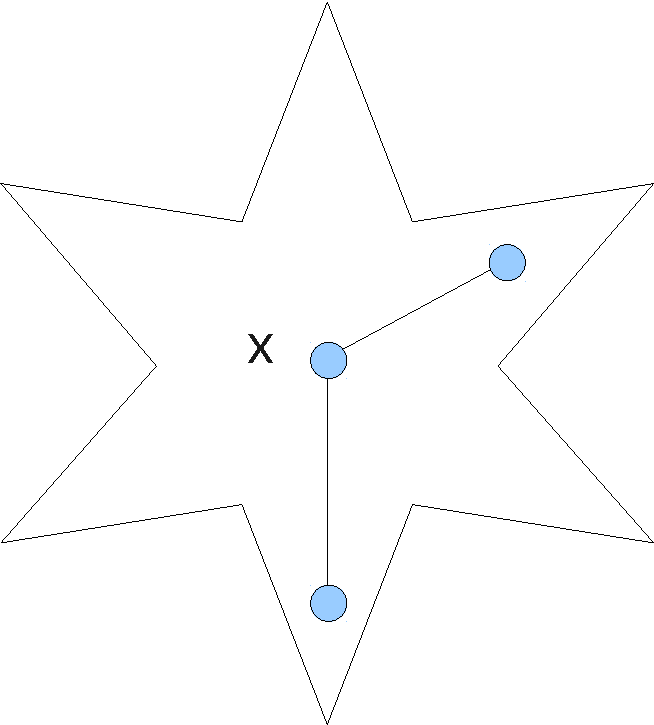
\includegraphics[scale=0.3]{images/ouvert_etoile.pdf}
\end{center}
\caption{Ouvert étoilé non convexe}\label{ch8:fig6}
\end{figure}
Une forme différentielle $f$ de degré $0$ donne par différentielle extérieure
une forme de degré 1:
\[
\omega = \frac{\partial f}{\partial x}dx + \frac{\partial f}{\partial y} dx
\]
Cette forme étant elle-même telle que $d\omega = 0$. On peut se demander s'il
existe une réciproque: si $\omega$ de degré $1$ vérifie $d\omega=0$,
peut-on trouver une fonction $f$ telle que $\omega=df$. Ceci est l'objet du
théorème de Poincaré.

\begin{fthm}
Soit $U$ un ouvert étoilé et $\omega = \alpha dx + \beta dy$ une forme de classe
$C^1$ sur $U$. Si $d\omega = 0$, il existe une forme de degré 0 sur $U$ telle
que $df = \omega$
\end{fthm}

\begin{proof}
Soit $p \in U$ un point par rapport auquel $U$ est étoilé. Soit $q$ un autre
point de $U$. On pose $v=(q-p)$ ; pour tout $t \in [0,1]$, $p + t v \in U$, on
pourra donc poser:
\[
f(p+v) = \int_{[0,1]} \alpha(p+tv).v_x + \beta(p+tv)v_y dt
\]
avec $v = v_x e_1 + v_y e_2$ ($e_1,e_2$ sont les vecteurs de base de
$\mathbb{R}^2$) En appliquant le théorème de dérivation sous le signe somme à la
fonction:
\[
h \mapsto f(p+t(v+he_1))
\]
on obtient:
\[
\frac{\partial f}{\partial x}(p+v) = \int_{[0,1]} t \frac{\partial
\alpha}{\partial x}(p+tv).v_x + \alpha(p+tv) + t \frac{\partial
\beta }{\partial x}(p+tv).v_y dt
\]
Si $d\omega = 0$, on a:
\[
\frac{\partial
\beta }{\partial x} = \frac{\partial
\alpha }{\partial y}
\]
et l'expression donnant la dérivée partielle devient:
\[
\frac{\partial f}{\partial x}(p+v) = \int_{[0,1]} t \left (\frac{\partial
\alpha}{\partial x}(p+tv).v_x +  \frac{\partial
\alpha }{\partial y}(p+tv).v_y \right) + \alpha(p+tv)  dt
\]
On a:
\[
\frac{d}{dt}\alpha(p+tv) = \left (\frac{\partial
\alpha}{\partial x}(p+tv).v_x +  \frac{\partial
\alpha }{\partial y}(p+tv).v_y \right)
\]
Et par intégration par parties:
\[
\frac{\partial f}{\partial x}(p+v) = \left[t\alpha(p+tv)\right]_0^1 =
\alpha(p+v)
\]
Prouvant bien que $\frac{\partial f}{\partial x} = \alpha$ pour tous les points
de $U$. On montrerait de même que $\frac{\partial f}{\partial x} = \beta$, ce
qui termine la preuve.
\end{proof}
Il est intéressant de noter que si l'hypothèse $d\omega =0$ n'est pas vérifiée,
on peut néanmoins construire $f$ et bien sûr calculer $df$ comme dans la preuve
précédente. Le terme résiduel qui dans ce cas rend différentes les formes $df$
et $\omega$ peut d'exprimer, avec quelques manipulations simples, uniquement en
fonction de $d\omega$, donnant en quelque sorte une généralisation du théorème.

La formule de Stokes, qui dans le cas de $\mathbb{R}^2$ porte aussi le nom de
théorème de Green-Riemann, est essentiellement une formule d'intégration par
parties pour les formes différentielles. Elle permet de transformer une
intégrale sur un ouvert de $\mathbb{R}^2$ en une intégrale sur son bord, au même
titre que la formule d'intégration par parties transforme une intégrale sur un
intervalle en une différence entre des valeurs prises sur ses extrémités.
La preuve de cette formule remarquable est délicate: les résultats présentés
ici seront volontairement limités à des cas simples, mais suffisamment généraux
pour les applications.

\begin{fprop}
Soit $U$ un ouvert de $\mathbb{R}^2$, $\Phi \colon V \to U$ un difféomorphisme
de classe $C^{k+1}$ et $\omega=\alpha dx + \beta dy$ une forme différentielle de
classe $C^k$ et de degré $1$ sur $U$. Soit enfin $\gamma$ un chemin de classe $C^1$ par morceaux
dont l'image est contenue dans $V$. On a:
\[
\int_{\Phi \circ \gamma} \omega = \int_{\gamma} \Phi^*\omega
\]
\end{fprop}

\begin{proof}
On notera encore $\Phi = \phi e_1 + \psi e_2$. 
Par définition:
\begin{align*}
\int_{\Phi \circ \gamma} \omega = & \int_{[0,1]}
\alpha\left((\Phi\circ\gamma)(t)\right) \frac{d}{dt}(\phi(\gamma(t))) \\
& + \beta\left((\Phi\circ\gamma)(t)\right) \frac{d}{dt}(\psi(\gamma(t))) dt
\end{align*}
Le théorème des fonctions composées donne, en notant $\gamma^\prime_x,
\gamma^\prime_y$ les composantes de $\gamma^\prime$ selon $e_1,e_2$:
\[
\frac{d}{dt}(\phi(\gamma(t))) = \frac{\partial \phi}{\partial
x}\gamma^\prime_x(t) + \frac{\partial \phi}{\partial
y}\gamma^\prime_y(t)
\]
et de même:
\[
\frac{d}{dt}(\psi(\gamma(t))) = \frac{\partial \psi}{\partial
x}\gamma^\prime_x(t) + \frac{\partial \psi}{\partial
y}\gamma^\prime_y(t)
\]
En regroupant les termes dans l'intégrale, on obtient:
\begin{align*}
& \int_{\Phi \circ \gamma} \omega = \\ &\int_{[0,1]}
\left(\alpha\left((\Phi\circ\gamma\right)(t)\frac{\partial \phi}{\partial
x}(t) +\beta\left((\Phi\circ\gamma\right)(t)\frac{\partial \psi}{\partial
x}(t)  + \right)\gamma^\prime_x(t) \\
& + \left(\alpha\left((\Phi\circ\gamma\right)(t)\frac{\partial \phi}{\partial
y}(t) +\beta\left((\Phi\circ\gamma\right)(t)\frac{\partial \psi}{\partial
y}(t)  + \right)\gamma^\prime_y(t) dt = \\
& \int_{\gamma} \Phi^*\omega
\end{align*}
\end{proof}

\begin{fprop}{(Théorème de Stokes élémentaire)}
Soit $\omega=\alpha dx + \beta dy$ une forme différentielle de classe $C^1$
définie sur un ouvert $U$ de $\mathbb{R}^2$, nulle en dehors d'un compact $K
\subset U$. On a:
\[
\int_{H^+} d \omega = \int_{\mathbb{R}} \alpha(x,0)dx
\]
Avec $H^+ = \mathbb{R} \times \mathbb{R}^+$ le demi-espace formé des points de
$\mathbb{R}^2$ à ordonnée positive.
\end{fprop}

\begin{proof}
La situation est résumée sur la figure \ref{ch8:fig7}. La preuve repose sur le
théorème de Fubini, et est élémentaire dans ce cas. On a par définition:
\[
d \omega = \left( \frac{- \partial \alpha }{\partial y} + \frac{\partial
\beta}{\partial x} \right) dx dy
\] 
et:
\[
\int_{H^+} d\omega = \int_{\mathbb{R}\times \mathbb{R}^+}  \left(-
\frac{\partial \alpha }{\partial y} + \frac{\partial \beta}{\partial x} \right) dxdy
\]
Le théorème de Fubini s'applique et on a:
\[
\int_{\mathbb{R}\times \mathbb{R}^+}-\frac{ \partial \alpha }{\partial
y}(x,y)dxdy = \int_{\mathbb{R}} \left(\int_{\mathbb{R}^+} -\frac{\partial \alpha
}{\partial y}(x,y)dy \right) dx
\]
Comme $\alpha$ est à support compact:
\[
\int_{\mathbb{R}^+} -\frac{\partial \alpha }{\partial
y}(x,y)dy = \alpha(x,0)
\]
De même par Fubini:
\[
\int_{\mathbb{R}\times \mathbb{R}^+}\frac{\partial \beta }{\partial
x}(x,y)dxdy = \int_{\mathbb{R}^+} \left(\int_{\mathbb{R}} \frac{\partial
\beta }{\partial x}(x,y)dx \right) dy
\]
Par compacité du support de $\beta$:
\[
\int_{\mathbb{R}} \frac{\partial
\beta }{\partial x}(x,y)dx = 0
\]
qui donne le résultat demandé.
 \begin{figure}[ht]
\begin{center}
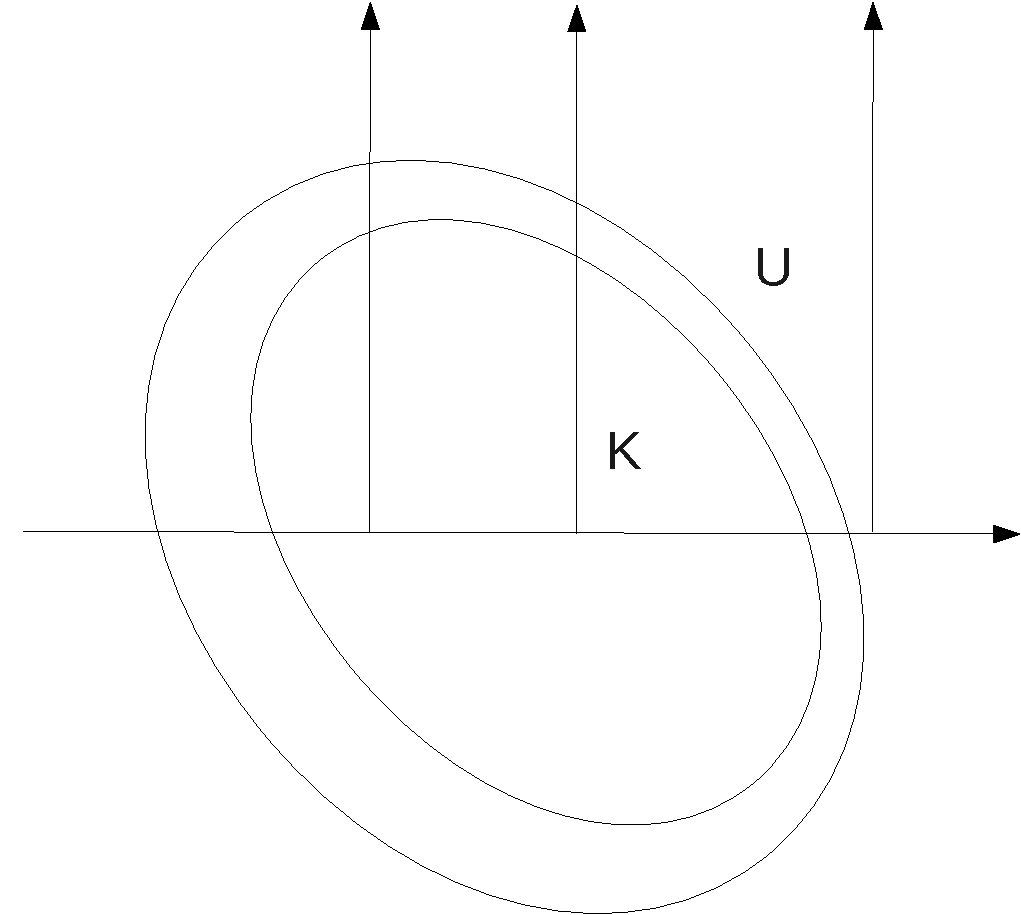
\includegraphics[scale=0.3]{images/stokes_elem.pdf}
\end{center}
\caption{Intégration de $d\omega$ par Fubini}\label{ch8:fig7}
\end{figure}
\end{proof}
On remarquera l'intégrale sur $\mathbb{R}^+$ peut être vue comme une intégrale de
chemin, en considérant pour cela un chemin correspondant à un segment de l'axe
réel et contenant le support de $\omega$.
On notera également que si le support de $\alpha$ a une intersection vide avec
l'axe réel positif, l'intégrale est nulle. Le cas général du théorème de Stokes
va s'obtenir en recollant des morceaux sur lesquels on le résultat élémentaire
pourra s'appliquer. La proposition suivante donne un procédé permettant un
découpage très régulier et s'utilise assez couramment.
\begin{fdefn}
On dira qu'un recouvrement ouvert $(U_i)_{i \in I}$ d'une partie $A \subset
\mathbb{R}^n$ est localement fini si tout point $x \in A$ possède un voisinage
ne rencontrant qu'un nombre fini d'ouverts du recouvrement.
\end{fdefn}
 \begin{fprop}{(Partitions de l'unité)}
 Soit $(U_i)_{i \in I}$ un recouvrement ouvert localement fini d'un ouvert $U
 \subset \mathbb{R}^n$. Il existe une famille d'applications $(\xi_i)_{j \in J}$ à
 valeurs dans $[0,1]$ telle que~:
 \begin{itemize}
   \item $\forall j \in J \exists i \in I \, supp(\xi_j) \subset U_i$.
   \item $\sum_{j \in J} \xi_j = 1$, où $1$ désigne l'application constante
   égale à 1.
 \end{itemize}
 \end{fprop}
La famille obtenue par la proposition précédente s'appelle partition de l'unité
subordonnée au recouvrement $(U_i)_{i \in I}$. La somme intervenant dans la
proposition est algébrique~: pour tout $x \in U$, il ne peut exister qu'un
nombre fini d'indices $j$ tels que $\xi_j(x) \neq 0$. Ceci apparaîtra clairement
au cours de la démonstration.
\begin{proof}
On remarquera tout d'abord qu'il existe une famille croissante de compacts
(pour la topologie induite sur $U$) $(K_n)_{n \in \mathbb{N}}$ telle que
$\cup_{n \in \mathbb{N}} K_n = U$ et $K_n \subset \overset{\circ}{K_{n+1}}$. Il suffit pour cela de prendre $K_n =
U \cap \overline{B(0,n)}$. Pour $n$ fixé, l'ensemble
$\tilde{K}_n = K_{n+1} - \overset{\circ}{K_{n}}$ est un compact car fermé
dans le compact $K_{n+1}$. On peut recouvrir $\tilde{K_n}$ par les ouverts
$O_{n,i} =  (\overset{\circ}{K}_{n+2} - K_{n-1}) \cap U_i$.Pour tout $x \in
O_{n,i}$, il est possible de trouver une boule ouverte $B(x,3r_x) \subset
O_{n,i}$. Soit $\psi \colon [0,1] \to [0,1]$ une application $C^\infty$ telle
que $\psi(0)=0, \psi(1)=1$ (voir le chapitre sur la transformation de Fourier
pour l'existence d'une telle fonction).
On définit $\theta_x$ par:
\[
\theta \colon y \mapsto \left \{
\begin{array}{cc}
1 & \text{ si } y \in B(x,r_x) \\
0 & \text{ si } y \in B(x,3r_x) - B(x,2r_x) \\
\psi\left(2 - \frac{\|y-x\|}{r_x}\right) & \text{ si } y \in B(x,2r_x) -
B(x,r_x)
\end{array}
\right .
\]
 Les boules ouvertes $B(x,r_x)$ forment un recouvrement ouvert du compact $\tilde{K}_n$, 
 on peut donc en extraire un sous-recouvrement fini déterminé par les points $x_{j,n}, i \in J_n$. 
 La collection $B(x_{j,n}, r_{x_{j,n}}), n \in
\mathbb{N}, j \in  J_n$ est dénombrable et vérifie les propriétés suivantes~:
\begin{itemize}
  \item Pour tout couple d'indices ${j,n}$, il existe $i \in I$ tel que
  $supp(\theta_{x_{j,n}}) \subset U_i$.
  \item Pour tout point $x \in U$, il n'existe qu'un nombre fini d'observables
  de la famille $\theta_{x_{j,n}}$ ne s'annulant pas en $x$.
  \item Pour tout point $x \in U$, il existe au moins une fonction
  de la famille $\theta_{x_{j,n}}$ ne s'annulant pas en $x$. 
\end{itemize}
Pour terminer la démonstration on pose~:
\[
\xi_{k,l} = \frac{\theta_{x_{k,l}}}{\sum_{n,j\in J_n} \theta_{x_{j,n}}} 
\]
\end{proof}

\begin{fthm}{(Théorème de Stokes)}
Soit $U$ un ouvert de $\mathbb{R}^2$ dont le bord est un lacet simple $\gamma$
de classe $C^1$ par morceaux, parcouru dans le sens trigonométrique. Soit $\omega=\alpha dx + \beta dy$ une forme différentielle
de classe $C^1$ définie sur $U$. On a: 
\[
\int_{U} d \omega = \int_{\gamma} \omega
\]
\end{fthm}

\begin{proof}
On ne donne ici qu'une idée de la preuve. Le lecteur pourra essayer de l'écrire
complètement. On supposera qu'en tout point $t$
de l'intervalle $[0,1]$, $\gamma^\prime(t) \neq 0$. En application du théorème d'inversion locale, on peut
trouver, pour tout point de $\gamma(t)$, un voisinage ouvert  $V$ de ce point et
un difféomorphisme $\Phi$ de classe $C^1$ sur un ouvert $W$ tel que
$\Phi(U\cap V) \in W\cap H^+$ et $\Phi(\gamma([0,1])\cap V)$ soit dans
l'intersection de $W$ avec l'axe réel. On peut imposer de plus
que $\Phi(\gamma(t))$ décrive un segment de l'axe réel d'abscisse croissante
avec $t$. L'image de $\gamma$ étant compacte, on peut extraire de la famille
précédente un sous-recouvrement fini. En y ajoutant l'ouvert $U$ lui-m\^eme, 
on peut construire une partition de l'unité subordonnée à cette famille. 
Sur la partie correspondant à $U$, l'intégrale de $d\omega$ est nulle.
 Sur les autres morceaux, on peut appliquer Stokes élémentaire: 
 les intégrales de chemin étant invariantes par difféomorphisme, on en déduit le
résultat.
\end{proof}
\begin{rem}
Une conséquence fondamentale du Théorème de Stokes est que l'intégrale d'une
forme fermée sur un lacet est nulle.
\end{rem}
\newpage
\leftline{\textbf{Un peu d'histoire \dots}}
\vskip 12pt
\begin{tabular}{ll}
\multicolumn{2}{l}{\textbf{Bernhard Riemann}} \\[10pt]
\begin{minipage}{0.2\linewidth}
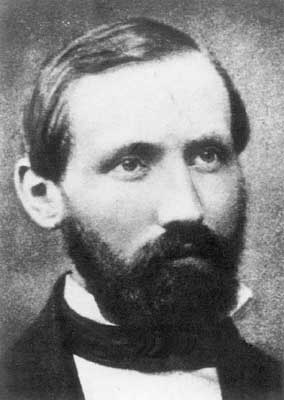
\includegraphics[scale=0.3]{images/Riemann.jpg}
\end{minipage}
&
\begin{minipage}{0.65\linewidth}
Né le  17 Septembre 1826 à Breselenz, mort le 20 Juillet 18666 à Semasca (Italie). Riemann est un des mathématiciens les plus importants de son époque et peut être de tous les temps. Durant sa courte carrière, il fonde la géométrie différentielle et contribue puissamment à l'étude des fonctions de la variable complexe. Il formalise la notion d'intégrale à partir de subdivisions de l'intervalle d'intégration.
\end{minipage}\\
\multicolumn{2}{l}{\textbf{Thomas Joannes Stieltjes}} \\[10pt]
\begin{minipage}{0.2\linewidth}
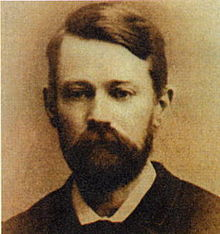
\includegraphics[scale=0.52]{images/Stieltjes.jpg}
\end{minipage}
& 
\begin{minipage}{0.65\linewidth}
Né le 29 décembre 1856 à Zwolle (Pays-Bas), mort le 31 décembre 1894 à Toulouse. Il travaillera sur les fractions continues, les formules de quadratures de Gauss et généralisera l'intégrale de Riemann.
\end{minipage}\\
\multicolumn{2}{l}{\textbf{Archimède}} \\[10pt]
\begin{minipage}{0.2\linewidth}
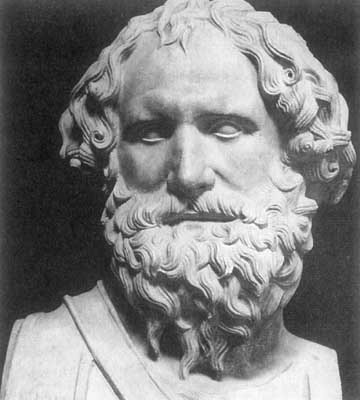
\includegraphics[scale=0.24]{images/archimede.jpg}
\end{minipage}
& 
\begin{minipage}{0.65\linewidth}
 Né à Syracuse  vers 287 av. J.-C. et mort à Syracuse en 212 av. J.-C. Génie universel, un des plus grands mathématiciens de tous les temps. Précurseur du calcul intégral, il invente la méthode d'approximation des périmètres par les chemins polygonaux. Sa défense du de Syracuse lors de son attaque par la flotte romaine et sa mort de la main d'un soldat sont particulièrement célèbres, ainsi que son exclamation "Eureka" (J'ai trouvé). On lui doit aussi l'invention de la vis, de l'écrou  et des roues dentées !
\end{minipage}\\
%\multicolumn{2}{l}{\textbf{Camille Jordan}} \\[10pt]
%\begin{minipage}{0.2\linewidth}
%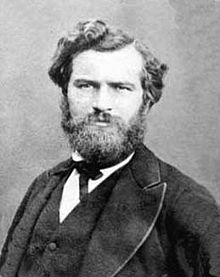
\includegraphics[scale=0.4]{images/Jordan.jpg}
%\end{minipage}
%& 
%\begin{minipage}{0.65\linewidth}
% Né à Lyon le 5 Janvier 1838 et mort à Paris le 22 Janvier 1922. Ingénieur de formation, il enseigne les mathématiques à l'école polytechnique et au collège de France. On lui doit un remarquable "cours d'analyse" ainsi que de nombreuses contributions en théorie des groupes.
%\end{minipage}
\end{tabular}
\vskip 12pt
\begin{tabular}{ll}
\multicolumn{2}{l}{\textbf{George Gabriel Stokes}} \\[10pt]
\begin{minipage}{0.2\linewidth}
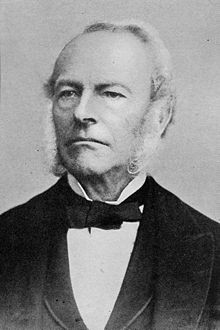
\includegraphics[scale=0.3]{images/Stokes.jpg}
\end{minipage}
&
\begin{minipage}{0.65\linewidth}
Né le  	13 août 1819 dans le Comté de Sligo (Irlande), mort le 1er février 1903 à Cambridge (Angleterre). Contribue à l'étude de la mécanique des fluide visqueux. Il explique la fluorescence de certains matériaux. Le théorème sur l'intégration des formes différentielles qui porte son nom est en réalité dû à Lord Kelvin (voir ci-dessous).
\end{minipage}\\
\multicolumn{2}{l}{\textbf{Lord Kelvin}} \\[10pt]
\begin{minipage}{0.2\linewidth}
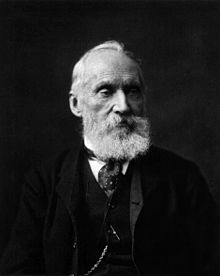
\includegraphics[scale=0.4]{images/Kelvin.jpg}
\end{minipage}
&
\begin{minipage}{0.65\linewidth}
Né le 26 juin 1824 à Belfast, mort le 17 décembre 1907 à
Largs. Physicien britannique très connu pour ses travaux en thermodynamique. On lui doit le second principe de cette science et l'échelle de température qui porte son nom. Il contribue aussi à l'électricité et à la mécanique et est un des pionniers de l'analyse vectorielle.  
\end{minipage}
\end{tabular}
\chapter{Différentiabilité dans $\mathbb{C}$}
\section{Rappels de calcul différentiel dans $\R^2$}
Les différentes notions présentées ici sont très classiques et probablement
déjà connues du lecteur. Dans toute cette section, $\Omega$ désignera un ouvert non vide de $\R^2$.
\subsection{Définitions}
\begin{fdefn}
Soit $g \colon \Omega \to \R^+$ une application. On dira que $f \colon \Omega \to \R^2$ est négligeable devant $g$ au
voisinage d'un point $x_0 \in \Omega$ si pour tout $\epsilon > 0$, il existe un voisinage $V_\epsilon$ de $x_0$ tel que:
\[
\forall x \in V_\epsilon, \, \|f(x)\| < \epsilon g(x)
\]
\end{fdefn}
\begin{notation}
On notera l'ensemble des applications négligeable devant $g$ au voisinage de $x_0$ par $o_{x_0}(g)$. 
\end{notation}
\begin{rem}
On condense très souvent la notation $o_{x_0}(g)$ en $o(g)$, le point $x_0$ étant sous-entendu.
\end{rem}
\begin{fdefn}\label{def:1.1}
Soit $\Omega \subset \R^2$ un ouvert et soit une application $f \colon \Omega \to \R^2$.
On dira que $f$ est différentiable en $x_0 \in \Omega$ si il existe une application affine $A \colon \R^2 \to \R^2$ telle
que $f-A \in o(\|x-x_0\|)$
\end{fdefn}
On a nécessairement $A(x_0)=f(x_0)$. En effet, par définition de l'ensemble $o(\|x-x_0\|)$, il existe un voisinage $U$ de $x_0$ tel que:
\[
\forall x \in U, \, \|f(x)-A(x)\| \leq \|x-x_0\|
\]
et la propriété s'ensuit en prenant $x=x_0$.
\begin{prop}
L'application $A$ est unique.
\end{prop}
\begin{proof}
Supposons l'existence d'une application affine $B$ vérifiant la même propriété que $A$. On de façon immédiate que $A-B \in o(\|x-x_0\|)$. Comme $A(x_0)=B(x_0)=f(x_0)$, l'application $\Theta \colon x \mapsto (A-B)(x-x_0)$ est linéaire.
Pour tout $\epsilon > 0$, il existe un voisinage $V_\epsilon$ de $x_0$ tel que:
\[
\forall x \in V_\epsilon, \|\Theta(x-x_0)\| \leq \epsilon \|x-x_0\|
\]
prouvant que la norme de l'application linéaire $\Theta$ est inférieure à $\epsilon$. Ceci étant vrai pour tout $\epsilon$, on en déduit que la norme de $\Theta$ est nulle, montrant ainsi que $\Theta=0$.
\end{proof}
L'application affine $A$ admet une écriture $A=f(x_0) + H(x-x_0)$. On peut ainsi reformuler la définition \ref{def:1.1} comme:
\begin{fdefn}\label{def:1.2}
Soit $\Omega \subset \R^2$ un ouvert et soit une application $f \colon \Omega \to \R^2$.
On dira que $f$ est différentiable en $x_0 \in \Omega$ si il existe une application linéaire $H \colon \R^2 \to \R^2$ telle que:
\[
f-f(x_0)-H(x-x_0) \in o(\|x-x_0\|)
\]
On dit que $H$ est l'application linéaire tangente à $f$ au point $x_0$.
\end{fdefn}
On fait le plus souvent l'abus de notation consistant à confondre \textbf{l'ensemble} $ o(\|x-x_0\|)$ avec un de ses éléments, pour écrire la relation entre $f$ et $H$  au voisinage de $x_0$ sous la forme:
\[
f(x) = f(x_0) + H(x-x_0) + o(\|x-x_0\|)
\]
Cette notation est la plus courante, mais se révèle parfois source d'erreurs: il faut toujours garder à l'esprit
que le terme $o(\|x-x_0\|)$ est en fait une \textbf{fonction} négligeable devant $\|x-x_0\|$ au voisinage de $x_0$.
On notera le plus souvent $H$ par $Df(x_0)$ ou $f^\prime(x_0)$.

Lorsqu'une application est différentiable en un point, elle y est bien représentée par une application linéaire et hérite de certaines de ses propriétés, dont la continuité, comme le montre la proposition ci-dessous:
\begin{fprop}\label{prop:1.1}
Soit $f \colon \Omega \to \R^2$ différentiable en $x_0$. $f$ est continue en $x_0$.
\end{fprop}
\begin{proof}
Soit $\epsilon > 0$. Il existe un voisinage $V_\epsilon$ de $x_0$ tel que:
\[
\forall x \in V_\epsilon, \, \left \| f(x) - f(x_0) -H(x-x_0) \right \| \leq \epsilon \|x-x_0\|
\]
Par ailleurs:
\[
\|f(x) -f(x_0)\| \leq \left \| f(x) - f(x_0) -H(x-x_0) \right \| + \left \| H(x-x_0) \right \|
\]
d où, pour $x \in V_\epsilon$:
\[
\|f(x) -f(x_0)\| \leq \left(\epsilon + \|H\| \right)\|x-x_0\|
\]
On en déduit le résultat.
\end{proof}
Lorsqu'une application est différentiable en tout point d'un ouvert $\Omega$, on dit plus simplement qu'elle est différentiable sur $\Omega$. Il est alors d'usage de noter l'application linéaire tangente à $f$ en $x$ par $f^\prime(x)$. L'application $f^\prime \colon x \in \Omega \mapsto f^\prime(x)$ s'appelle \textbf{application dérivée} de $f$.

\begin{fdefn}
Une application $f \colon \Omega \to \R^2$ différentiable sur $\Omega$ et d'application dérivée continue est dite de classe $C^1(\Omega)$.
\end{fdefn}
\subsection{Interprétation géométrique}

Un endomorphisme de $\R^2$ se représente comme une transformation du plan. Étant linéaire, elle agira sur un segment de droite pour donner un autre segment de droite. La figure \ref{fig:trlin} donne un exemple de l'action d'un endomorphisme du plan sur une grille uniforme ; on notera en particulier que la déformation préserve les parties droites.
\begin{figure}[ht]
\centering
\begin{subfigure}[b]{0.45\textwidth}

\includegraphics[width=\textwidth]{images/ima1.png}
\caption{Grille initiale}
\label{fig:uni_mesh}
\end{subfigure}
\begin{subfigure}[b]{0.45\textwidth}
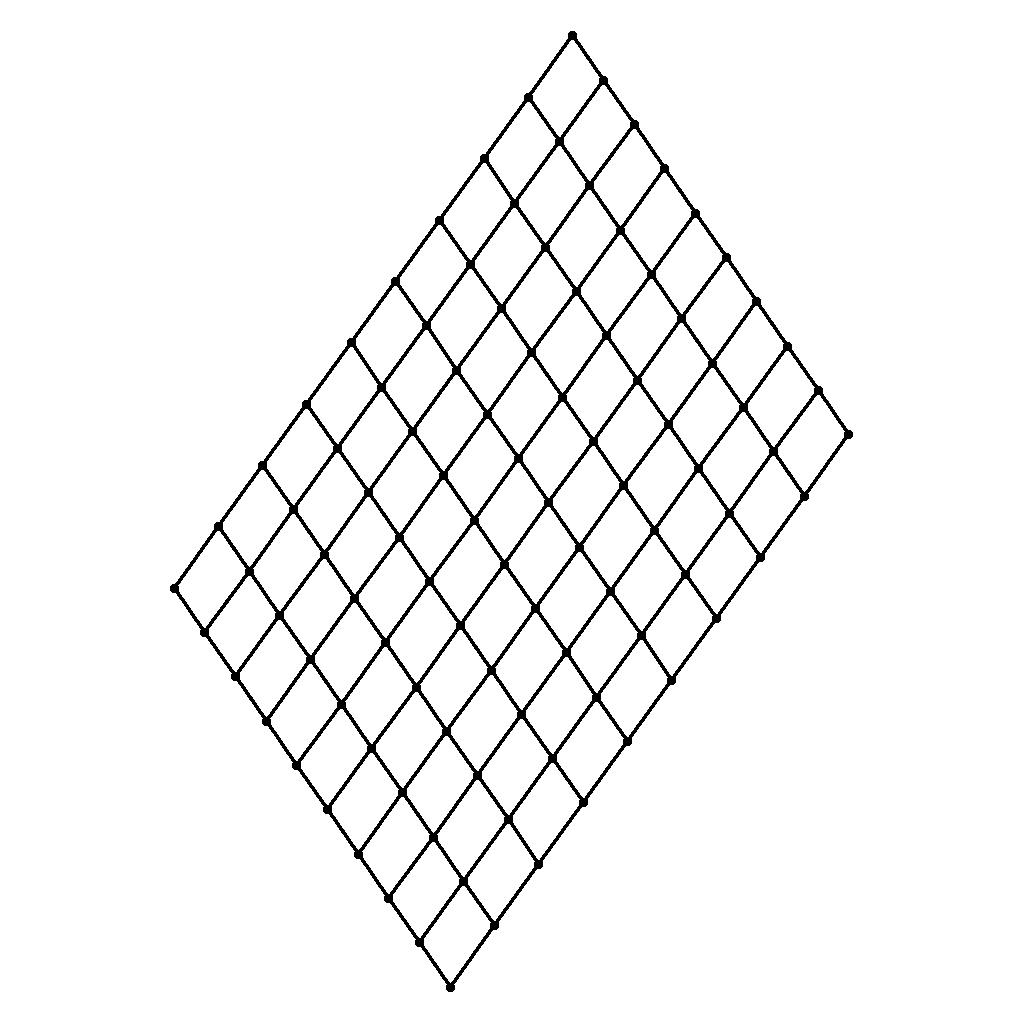
\includegraphics[width=\textwidth]{images/ima2.png}
\caption{Grille Transformée}
\label{fig:trlin_mesh}
\end{subfigure}
\caption{Transformation linéaire}\label{fig:trlin}
\end{figure}
A contrario, une application quelconque de $\R^2$ dans lui-même pourra donner des résultats notablement différents, tel  que celui présenté en figure \ref{fig:trnlin}
\begin{figure}[ht]
\centering
\begin{subfigure}[b]{0.45\textwidth}

\includegraphics[width=\textwidth]{images/ima1.png}
\caption{Grille initiale}
\label{fig:uni_mesh}
\end{subfigure}
\begin{subfigure}[b]{0.45\textwidth}
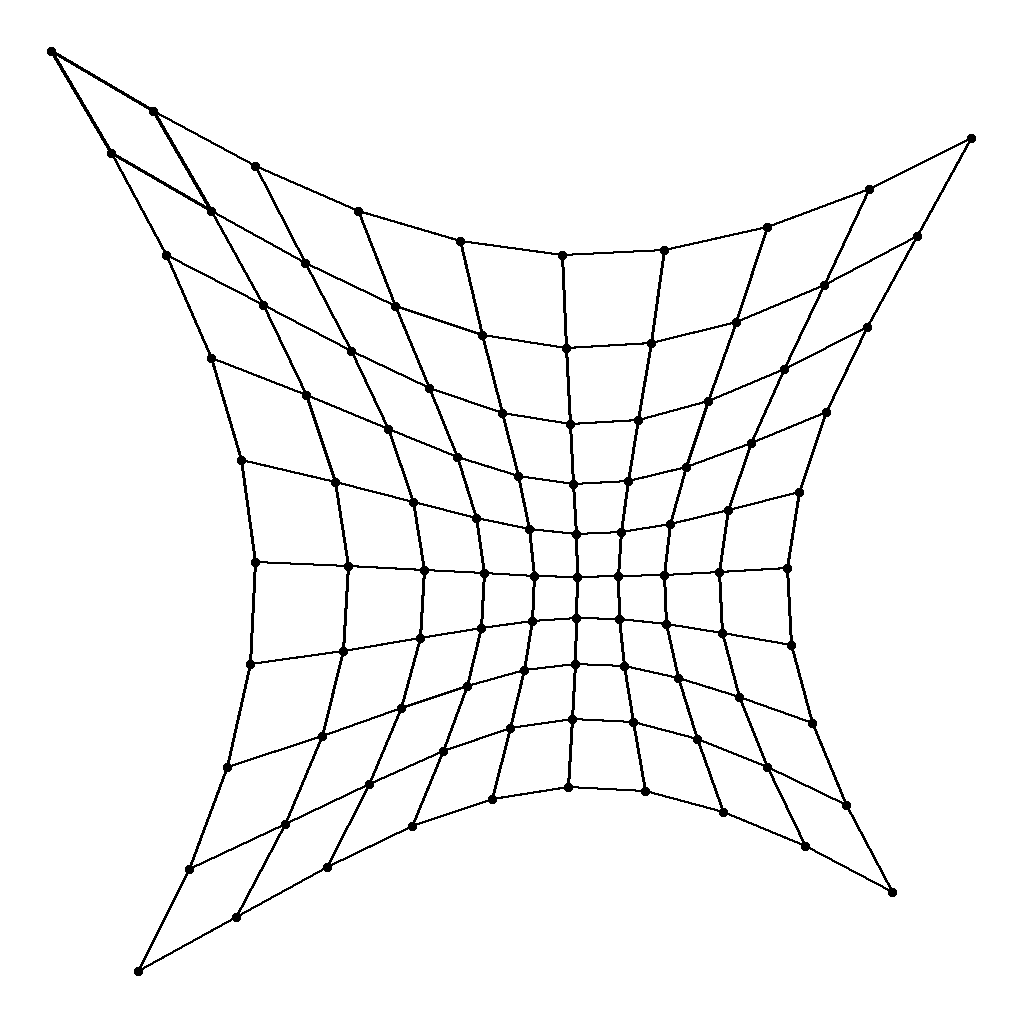
\includegraphics[width=\textwidth]{images/ima3.png}
\caption{Grille Transformée}
\label{fig:trnlin_mesh}
\end{subfigure}
\caption{Transformation non linéaire}\label{fig:trnlin}
\end{figure}

Dans le cas d'une application différentiable en un point, on peut d'une certaine façon faire coïncider localement la transformation non linéaire et l'endomorphisme qui lui est tangent en un point. Ceci est représenté sur la figure \ref{fig:diffapprox} où l'on remarque une très bonne coïncidence au voisinage du point où la différentielle est calculée.

\begin{figure}[ht]
\centering
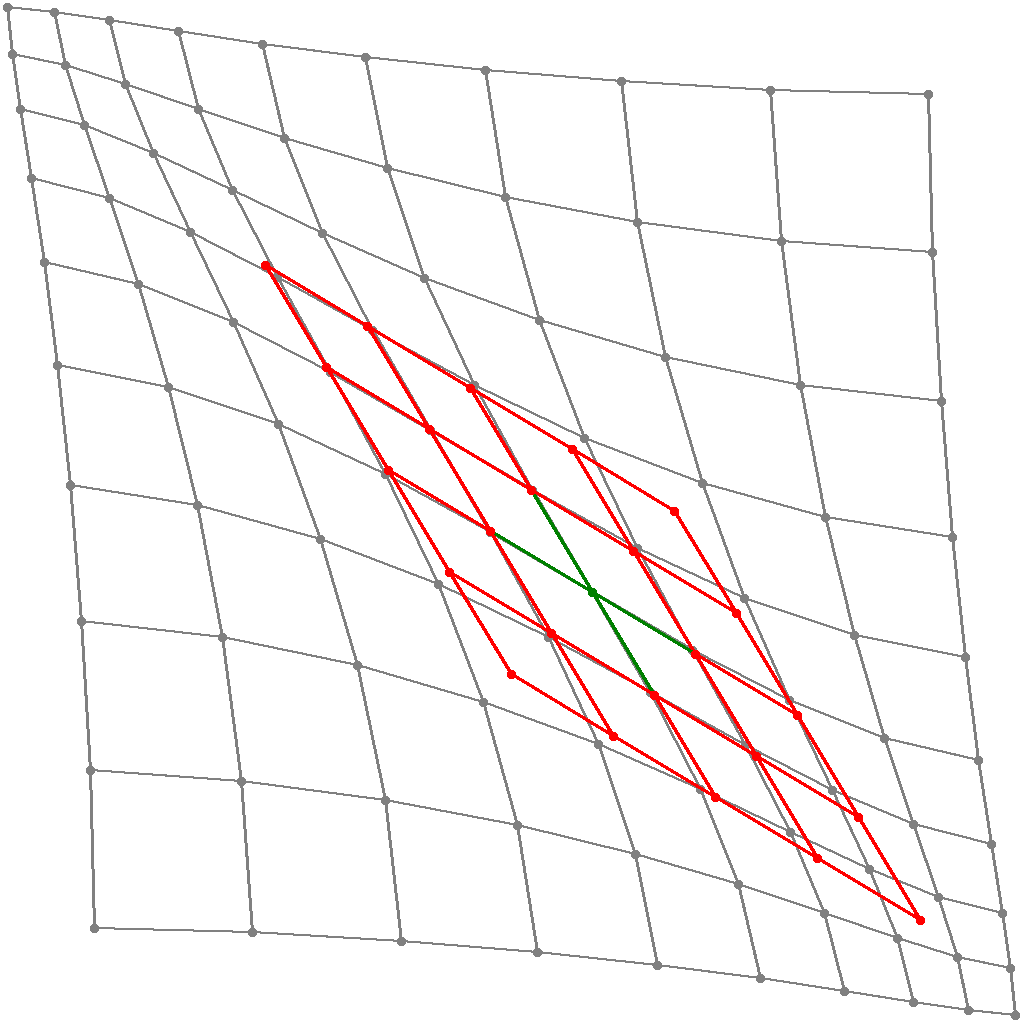
\includegraphics[width=0.5\textwidth]{images/ima4.png}
\caption{Approximation par une application affine}\label{fig:diffapprox}
\end{figure}

\subsection{Inversion locale}

Les propriétés de l'application linéaire tangente ne reflètent pas toujours celles de l'application initiale. On remarque qu'une application telle que $f \colon  x \in \R \mapsto x^3$ est inversible sur $\R$ tout entier, mais que sa dérivée en 0 est 0, donc non inversible. Pour obtenir une meilleure adéquation entre le comportement de l'application et de son modèle local, on imposera souvent une condition plus forte que la différentiabilité simple. 

\begin{fdefn}\label{def:strict_diff}
Soit $f \colon \Omega \to \R^2$. On dira que $f$ est strictement différentiable en $x_0 \in \Omega$ si l'on peut trouver un voisinage $V$ de $x_0$ et une application linéaire $H$ tels que:
\[
\forall (x,y) \in V^2, \, f(y) = f(x) + H(y-x) + o_{x_0}\left(\|y-x\|\right)
\]
\end{fdefn}

La différentiabilité stricte implique la différentiabilité simple, il suffit pour cela de considérer des couples de la forme $(x,x_0)$, mais la réciproque est fausse. L'intérêt majeur d'introduire cette notion réside dans le théorème suivant, dit d'inversion locale.

\begin{fthm}
Soit $f \colon \Omega \to \R^2$ une application strictement différentiable en $x_0 \in \Omega$. Si $f^\prime(x_0)$ est inversible, alors il existe un voisinage ouvert $U$ de $x_0$ et un voisinage ouvert $W$ de $f(x_0)$ tels que $f$ soit un homéomorphisme de $U$ sur $W$. De plus, $f^{-1}$ est strictement dérivable en $f(x_0)$ et on a $Df^{-1}(f(x_0)) = \left(f^{\prime}\right)^{-1}(x_0)$.
\end{fthm}
La preuve est très classique. Elle est détaillée ci-dessous en raison de son caractère constructif qui fournit un algorithme numérique permettant d'inverser en un point une application. Un résultat intermédiaire fondamental, le théorème du point fixe, va être maintenant rappelé en préliminaire à la preuve proprement dite.

\begin{fthm} \label{thm:pt_fixe}
Soit $E$ un espace de Banach (i.e. espace vectoriel normé complet pour la topologie induite par la norme). Soit $f$ une application de $E$ dans $E$ telle qu'il existe un réel $1 > k > 0$ vérifiant:
\[
\forall (x,y) \in E, \, \|f(x)-f(y)\| \leq k \|x-y\|
\]
alors il existe un unique $x_0 \in E$ tel que $f(x_0)=x_0$.
\end{fthm}
Une application vérifiant l'hypothèse de majoration ci-dessus est dite contractante. Il est important de bien noter que le réel $k$ doit être strictement inférieur à 1. 
\begin{proof}
Soit $x$ un point quelconque de $E$. On pose, pour tout entier $n$: $x_0 = x, x_{n+1}=f(x_n)$. Pour tout entier $n \geq 1$, on a:
\[
\left\| x_{n+1}-x_n \right \| = \left\| f(x_n)-f(x_{n-1}) \right \| \leq k \left\| x_n-x_{n-1} \right \|
\leq k^n \left\| x_1-x_0 \right \| 
\]
on en déduit que pour tout couple d'entiers $1 \leq p < q$:
\[
\left\| x_q - x_p \right \| \leq \sum_{i=p}^{q-1} \left\| x_{i+1} - x_i \right \| \leq \sum_{i=p}^{q-1} k^i \left\| x_1-x_0 \right \| \leq \frac{k^p}{1-k} \left\| x_1-x_0 \right \|
\]
Prouvant ainsi que la suite $(x_n)_{n \in \N}$ est de Cauchy. Comme $E$ est un espace complet, elle admet une limite $x^*$ dans $E$. $f$ est Lipschitzienne, donc continue. On a ainsi:
\[
x^* = \lim_{n \to +\infty } x_{n+1} = \lim_{n \to +\infty} f(x_n) = f\left( \lim_{n \to +\infty} x_n \right)
=f(x^*)
\]
montrant que $x^*$ est un point fixe de $f$. L'unicité s'obtient facilement en supposant l'existence de deux points fixes distincts $x^*, x^{*\prime}$. La majoration vérifiée par $f$ donne:
\[
\|x^* - x^{*\prime}\|= \|f(x^*) - f(x^{*\prime})\| \leq k \|x^* - x^{*\prime}\|
\] 
ce qui est impossible car $k < 1$.
\end{proof}
\begin{rem}
Le théorème du point fixe est remarquable sur deux points: 
\begin{itemize}
\item La convergence a lieu indépendamment du point de départ. 
\item La suite d'approximation du point fixe donne un algorithme explicite de calcul.
\end{itemize}
\end{rem}
On peut maintenant revenir à la preuve du théorème d'inversion locale qui sera elle aussi constructive.
\begin{proof}
L'idée principale est d'utiliser pour l'inversion le modèle linéaire fourni par la différentielle en $x_0$ en lieu et place de l'application $f$. 
Soit $V$ un voisinage de $x_0$ dans lequel l'application $f$ vérifie la condition de stricte différentiabilité:
\[
\forall (p,q) \in V, \, f(p)=f(q) +Df(x_0)(p-q) + o_{x_0}\left(\|p-q\|\right)
\]
 avec~:
 \[
  \left\|o_{x_0}\left(\|p-q\|\right)\right\| \leq \frac{\|Df(x_0)\|}{2} \|p-q\|
 \]
Soit $y \in f(V)$. On pose, pour tout $x \in V$:
\[
\Theta_y(x) = x + Df^{-1}(x_0)\left(y-f(x)\right)
\]
On notera que $\Theta_y$ modifie $x$ de telle façon que l'on aurait $y=f(\Theta_y(x))$ si $f$ était une application affine. On espère ici que le modèle linéaire donné par la différentielle sera suffisamment bon pour que $f(\Theta_y(x))$ soit plus proche de $y$ que ne l'était $x$. L'application $\Theta_y$ est contractante. Pour tout couple $(x,z)$ de points de $V$ on a:
\begin{align*}
\left\|\Theta_y(x) - \Theta_y(z)\right\| &  = \left\|z-x + Df^{-1}(x_0)\left(f(x)-f(z)\right) \right \| \\
& = \left\|Df^{-1}(x_0)\left( Df(x_0)(z-x) + f(x)-f(z)\right) \right \| \\
& \leq \|Df^{-1}(x_0)\|  \left\|o_{x_0}\left(\|z-x\|\right)\right\| \leq \frac{1}{2} \|z-x\|
\end{align*}
De plus, pour $x \in V$:
\begin{align*}
&\left\| \Theta_y(x) - x_0 \right \|  = \left \| x-x_0 + Df^{-1}(x_0)\left(y-f(x)\right) \right \| \\
& \leq \left \| x-x_0 + Df^{-1}(x_0)\left(f(x_0)-f(x) \right) \right \| + \left\| Df^{-1}(x_0)\left(y-f(x_0)\right)\right\| \\
& \leq \frac{\|x-x_0\|}{2} + \|Df^{-1}(x_0)\|\|y-f(x_0)\|
\end{align*}
d'où l'on déduit que si l'on choisi $x$ dans une boule $B(x_0,r) \subset V$, $\Theta_y(x)$ sera encore dans cette boule sous réserve que $y$ appartienne à la boule de centre $f(x_0)$ et de rayon $\eta=\|Df(x_0)\|r/2$. Sous ces conditions, le théorème du point fixe montre qu'il existe $z$ tel que $\Theta_y(z)=z$, qui équivaut à $f(z)=y$. En choisissant comme domaine de départ une boule ouverte $B(x_0,r\prime)$ contenue dans l'ouvert $B(x_0,r) \cap f^{-1}(B(f(x_0,\eta)))$, on assure que $f$ réalise une bijection sur $f(B(x_0,r\prime))$.

Soient $y,z$ deux points de $f(B(x_0,r\prime))$. En remarquant que:
\[
\Theta_y(f^{-1}(y))=f^{-1}(y), \Theta_z(f^{-1}(z))=f^{-1}(z)
\]
il vient:
\begin{align*}
& \|f^{-1}(y) - f^{-1}(z) \| \leq \\ &
\| \Theta_z(f^{-1}(z)) -\Theta_y(f^{-1}(z)) \| + \| \Theta_y(f^{-1}(z))-\Theta_y(f^{-1}(y)) \| \\
& \leq  \| \Theta_z(f^{-1}(z)) -\Theta_y(f^{-1}(z)) \|  + \frac{1}{2} \|f^{-1}(y) - f^{-1}(z) \|
\end{align*}
d où l'on tire:
\[
 \frac{1}{2} \|f^{-1}(y) - f^{-1}(z) \| \leq  \| \Theta_z(f^{-1}(z)) -\Theta_y(f^{-1}(z)) \| 
\]
Comme:
\[
\| \Theta_z(f^{-1}(z)) -\Theta_y(f^{-1}(z)) \|  = \| Df^{-1}(x_0) (z-y) \| \leq \| Df^{-1}(x_0)\| \|(z-y) \| 
\]
on a:
\[
 \|f^{-1}(y) - f^{-1}(z) \| \leq  2 \| Df^{-1}(x_0)\| \|(z-y) \| 
\]
prouvant le caractère lipschitzien de $f^{-1}$.

Enfin:
\begin{align*}
& \|f^{-1}(z)-f^{-1}(y) +Df^{-1}(x_0)(y-z)\| \leq \\
& \| Df^{-1}(x_0)\| \| y-z+Df(x_0)\left(
f^{-1}(z) - f^{-1}(y)\right) \|
\end{align*}
Le terme $y-z+Df(x_0)\left(f^{-1}(z) - f^{-1}(y)\right)$ est dans $o_{x_0}(\|f^{-1}(z)-f^{-1}(y)\|)$, mais aussi 
dans $o_{f(x_0)}(\|z-y\|)$, $f^{-1}$ étant lipschitzienne. On en déduit la stricte différentiabilité de $f^{-1}$, avec une différentielle en $f(x_0)$ égale à $Df^{-1}(x_0)$.
\end{proof}
\begin{rem}
Le théorème d'inversion locale est vrai dans le cadre beaucoup plus général des espaces de Banach.
\end{rem}

La proposition suivante permet d'utiliser le théorème d'inversion locale dans le cadre des applications de classe $C^1(\Omega)$, qui sont plus aisées à caractériser.
\begin{fprop}
Une application de classe $C^1(\Omega)$ est strictement différentiable en tout point de $\Omega$.
\end{fprop}
\begin{proof}
Soit $x_0\in \Omega$ et soit $\epsilon > 0$. Par continuité de $f^\prime$, il existe un voisinage $V_\epsilon$ de 
$x_0$ tel que pour tout $y$ dans $V_\epsilon$:
\[
\left\| f^{\prime}(y)-f^\prime(x_0) \right\| \leq \frac{\epsilon}{2} 
\]
Pour tout couple de points $(y,z)$ de $V_\epsilon$:
\begin{align*}
f(z)-f(y)-f^\prime(x_0)(z-y) & = \left(f(z)-f(y)-f^\prime(y)(z-y) \right)  \\
 & + \left(f^\prime(y)-f^\prime(x_0)\right)(z-y)
\end{align*}
Le premier terme du membre de droite est dans $o(\|z-y\|)$ en vertu de la différentiabilité de $f$ et quitte à réduire $V_\epsilon$, on peut supposer dans perte de généralité qu'il est majoré par $\epsilon \|z-y\| /2$. Le second terme est majoré par la même quantité, on a donc:
\[
\left\|f(z)-f(y)-f^\prime(x_0)(z-y)\right \| \leq  \epsilon \|z-y\|
\]
montrant la stricte différentiabilité de $f$ en $x_0$.
\end{proof}
La proposition précédente est locale: on peut supposer la différentiabilité au voisinage de $x_0$ et la continuité de $f^\prime$ en ce point pour assurer la strict différentiabilité en $x_0$.

On utilise le plus souvent dans le cadre $\R^2$ la proposition suivante pour montrer le caractère $C^1$ d'une application. 

\begin{fprop}
Soit $f \colon \Omega \to \R^2$. Si les dérivées partielles de $f$ existent et sont continues, alors $f$ est de classe $C^1(\Omega)$.
\end{fprop}
\begin{danger}
\begin{rem}
Attention, il s'agit d'une condition suffisante mais non nécessaire.
\end{rem}
\end{danger}

\subsection{Calcul numérique}
Le théorème d'inversion locale est constructif: il donne un algorithme explicite permettant d'approcher l'inverse d'une fonction point par point. On utilise très fréquemment cette remarquable propriété dans des applications de calcul numérique.
Nous présentons ici un code écrit en python réalisant l'implémentation informatique de ce qui vient d'être indiqué. Le code sera organisé autour d'une boucle dans laquelle seront exécutées les itérations du point fixe. Pour rester dans le cadre de ce cours, on se limitera aux cadre des applications de $\R^2$ dans $\R^2$, il est ainsi possible d'inverser directement les matrices jacobiennes. 

\begin{verbatim}
import math

# fonction à inverser
# x: vecteur de réels de taille 2
# return: vecteur de réels de taille 2
def my_func(x): 
    return [x[0]*x[0] + x[1]*x[1], x[0]*x[1]]
    
# matrice jacobienne de l'application à inverser
# x: vecteur de réels de taille 2
# return: matrice de réels de taille 2x2
def my_jac(x):
    return [[2 * x[0],2 * x[1]],[x[1],x[0]]]

# inversion d'une matrice 2x2
# une exception est levée lorsque la matrice est presque
# singulière à la precision machine
# a: matrice 2x2 de reels
# return: matrice 2x2  
def mat_inv(a):
    det = a[0][0] * a[1][1] - a[0][1] * a[1][0]
    if math.fabs(det) < 1e-8:
        # la matrice est presque singulière a la péecision machine
        # on lève une exception, au plus simple !
        raise ArithmeticError
    # inversion "à la main" de la matrice jacobienne
    return [[a[1][1]/det, -a[0][1]/det],[-a[1][0]/det, a[0][0]/det]]
    
# fonction réalisant une itération de point fixe 
# le premier argument représente le point où l'inverse
# est recherché.
# le second argument est le point candidat courant
# les arguments f,df representent respectivement la fonction
# à inverser et sa matrice jacobienne
# y: vecteur de réels de taille 2
# x: vecteur de réels de taille 2
# f: fonction à inverser
# ijac: inverse de la matrice jacobienne de la fonction
# à inverser au point de référence
# return: liste dont le premier &lement est un vecteur de 
# réels de taille 2, résultat de l'evaluation et le second
# argument est un réel donnant la norme de l'erreur commise.
def my_theta(y,x,f,ijac):
# évaluation de la fonction
    fx = f(x)
    # vecteur d'erreur 
    err=[y[0]-fx[0],y[1]-fx[1]]
    # terme correctif du modèle linéarisé
    a = ijac[0][0] * err[0] + ijac[0][1] * err[1]
    b = ijac[1][0] * err[0] + ijac[1][1] * err[1]
    # résultat final
    return [[x[0] + a, x[1] + b],math.sqrt(err[0] * err[0] + err[1] * err[1])]
    
# fonction réalisant une iteration de point fixe selon 
# la methode améliorée
# le premier argument représente le point ou l'inverse 
# est recherché.
# le second argument est le point candidat courant
# les arguments f,df representent respectivement 
# la fonction  à inverser et sa matrice jacobienne
# y: vecteur de reels de taille 2
# x: vecteur de reels de taille 2
# f: fonction à inverser
# df: jacobienne de la fonction a inverser
# return: liste dont le premier element est un vecteur de 
# réels de taille 2, résultat de l'evaluation 
# et le second argument est un réel donnant la norme
# de l'erreur commise.
def my_theta_i(y,x,f,df):
# évaluation de la fonction et de sa jacobienne
    fx = f(x)
    dfx = df(x)
    # inversion de dfx avec test de singularité
    idfx = mat_inv(dfx)           
    # vecteur d'erreur 
    err=[y[0]-fx[0],y[1]-fx[1]]
    # terme correctif du modele linéarisé
    a = idfx[0][0] * err[0] + idfx[0][1] * err[1]
    b = idfx[1][0] * err[0] + idfx[1][1] * err[1]
    # résultat final
    return [[x[0] + a, x[1] + b],math.sqrt(err[0] * err[0] + err[1] * err[1])]

# le code principal

# choix du type d'iteration

use_improved_iteration = False

# point de calcul initial, choisi hors des droites
#  y=x, y=-x sur lesquelles la matrice jacobienne 
# est singulière

x0 = [1.0, 2.0]

# point de référence pour l'application du théorème 
# d'inversion locale
# Il doit être assez proche de x0 pour que les itérations convergent

p = [1.2, 1.5]

# l'inverse du jacobien au point considéré

ijac = mat_inv(my_jac(p))

# la valeur image

y = my_func(x0)

# point de départ des itérations, toujours 
# hors des points singuliers

x=[2.0, 3.0]

# itération de point fixe jusqu'a éeduction suffisante de l'erreur

if use_improved_iteration:
    # itération améliorée
    res = my_theta_i(y, x, my_func, my_jac)
else:
    # itération standard
    res = my_theta(y, x, my_func, ijac)
while res[1] > 1e-8:
    # point courant = point de l'itération précédente
    x = res[0]
    # affichage du l'erreur et du point courant
    print(res[1],res[0])
    # nouvelle itération
    if use_improved_iteration:
        res = my_theta_i(y, x, my_func, my_jac)
    else:
        res = my_theta(y, x, my_func, ijac)
\end{verbatim}
On pourra facilement changer les valeurs des points de référence et de départ pour voir les différences de comportement du code.
Une méthode améliorée dans laquelle la valeur de la matrice jacobienne est recalculée à chaque itération est également disponible: il suffit pour cela de changer de \texttt{False} à \texttt{True} la valeur de la variable \texttt{use\_improved\_iteration}. Cet algorithme modifié est celui qui est employé en pratique. Il permet entre autres choses de retrouver des valeurs de paramètres inconnus à partir d'observations: il est ainsi possible en observant certains paramètres au cours d'un vol d'en déduire par exemple les coefficients aérodynamiques d'un avion. 
\vskip 12pt
\leftline{\textbf{Un peu d'histoire \dots}}
\vskip 12pt
\begin{tabular}{ll}
\multicolumn{2}{l}{\textbf{Gottfried Wilhelm von Leibniz}} \\[10pt]
\begin{minipage}{0.2\linewidth}
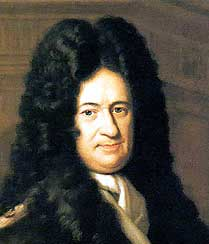
\includegraphics[scale=0.3]{images/Gottfried_Wilhelm_von_Leibniz.jpg}
\end{minipage}
&
\begin{minipage}{0.65\linewidth}
Né le  1 juillet 1646 à Liepzig, mort le 14 novembre 1716 à Hanovre, Gottfried Liebniz est un esprit universel,
philosophe, mathématicien, logicien, juriste et diplomate. Il partage avec Isaac Newton la paternité du calcul différentiel et intégral, une controverse sur l'antériorité de la découverte ayant opposé les deux hommes. La notation de Liebniz $\partial f$ est celle qui a été retenue par les mathématiciens, de même que le symbole $\int$ pour l'intégrale.
\end{minipage}\\
\multicolumn{2}{l}{\textbf{Isaac Newton}} \\[10pt]
\begin{minipage}{0.2\linewidth}
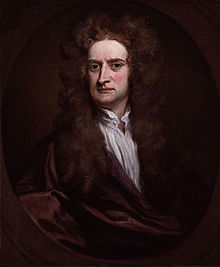
\includegraphics[scale=0.3]{images/isaac_newton.jpg}
\end{minipage}
& 
\begin{minipage}{0.65\linewidth}
Né le  4 janvier 1643 à Woolsthorpe, mort le 31 mars 1727 à Kensington est un scientifique et philosophe anglais surtout connu pour sa loi de la gravitation universelle. Il a apporté de nombreuses contributions dans le domaine des mathématiques, en particulier la formule du binôme et l'algorithme de recherche des zéros d'une fonction qui porte son nom. Ses travaux sur le calcul infinitésimal on été publiés postérieurement à ceux de Liebniz ce qui a donné lieu à son époque à une dispute sur l'attribution de cette découverte. On lui doit également de nombreux travaux en optique.
\end{minipage}\\
\multicolumn{2}{l}{\textbf{Stefan Banach}} \\[10pt]
\begin{minipage}{0.2\linewidth}
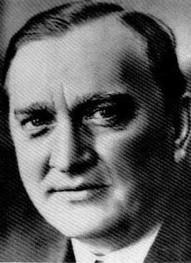
\includegraphics[scale=0.3]{images/banach.jpg}
\end{minipage}
& 
\begin{minipage}{0.65\linewidth}
Né le 30 mars 1892 à Ostrowsko, mort le 31 août 1945 à Lviv. Banach est un mathématicien fécond, fondateur de l'analyse fonctionnelle. Ses travaux sur les espaces vectoriels topologiques le conduisent à définir les espaces qui portent maintenant son nom. On lui doit également le théorème du point fixe pour les applications contractantes, ainsi que le célèbre paradoxe de Banach-Tarski.
\end{minipage}
\end{tabular}

\section{L'espace vectoriel des nombres complexes}
L'étude des propriétés des applications de $\C$ dans $\C$ est un domaine particulièrement fécond des mathématiques qui a conduit à de très nombreux résultats en analyse. Les remarquables propriétés différentielles de ces applications en ont popularisé l'usage bien au delà du cadre des mathématiques. Dans toutes les applications de physique demandant la résolution d'équations de type Poisson, les techniques issues de la théorie des fonctions de la variable complexe étaient les méthodes de choix jusqu'à l'avènement des calculateurs électroniques. On les utilise encore aujourd'hui lorsque l'on souhaite une expression analytique de la solution, ou tout simplement pour la simplicité et l'élégance.  

L'ensemble $\C$ des nom\-bres complexes possède deux structures naturelles d'espace vectoriel, l'une d'espace vectoriel complexe et l'autre d'espace vectoriel réel. $\C$ considéré comme espace vectoriel sur lui-même est de dimension $1$ alors qu'il est de dimension 2 en tant qu'espace réel. Dans de dernier cas, il est isomorphe à $\R^2$ par l'isomorphisme canonique $(x,y) \in \R^2 \mapsto x + i y$. Pour un complexe $z=x+iy$, on rappelle que le point $(x,y)$ est appelé \textbf{affixe} de $z$.

Soit $f : \Omega \subset \mathbb{C} \to \mathbb{C}$ une fonction de la variable complexe. En posant $z = x + iy$, on peut écrire~:
\[
f(z) = P(x,y) + i Q(x,y)
\]
avec $P$ et $Q$ les parties réelle et imaginaire de $f$. On peut par cette décomposition associer à l'application initiale $f$ une application de $\R^2$ dans $\R^2$ que l'on continuera à noter $f$:
\[
f \colon (x,y) \mapsto \left(P(x,y), Q(x,y)\right)
\]
Dans la suite, on passera librement d'une notation à une autre en fonction du contexte. 

Muni de la norme induite par la norme euclidienne de $\mathbb{R}^2$,
$\mathbb{C}$ est un espace de Banach réel. La norme d'un nombre
complexe $z$ est appelée \textbf{module} de $z$, noté $|z|$.
Le module est aussi une norme sur $\C$ considéré comme espace vectoriel sur lui-même. 

\begin{rem}
Le produit usuel de deux nombres complexes fait de $ \mathbb{C}$ une
algèbre sur lui-même. La relation $\forall (z_1,z_2) \in \mathbb{C}^2,
|z_1 z_2| = |z_1||z_2|$ montre que l'algèbre en question est
normée. Comme $\mathbb{C}$ est aussi un espace de Banach pour la norme
$|.|$, on dit qu'il s'agit d'une algèbre de Banach.
\end{rem}
Il est important de noter que la distinction entre $\mathbb{C}$ considéré comme
$\mathbb{R}$-espace vectoriel et $\mathbb{C}$-espace vectoriel a une conséquence
fondamentale sur les applications linéaires qui ont pour domaine l'un ou l'autre
de ces espaces.
\begin{fprop}
Soit $f \colon \mathbb{C} \to \mathbb{C}$ une application $\mathbb{C}$-linéaire.
Il existe un complexe $\lambda \in \mathbb{C}$ tel que pour tout $z \in
\mathbb{C}$, $f(z) = \lambda z$
\end{fprop}
\begin{proof}
La preuve est plus courte que l'énoncé. Si $f$ est $\mathbb{C}$-linéaire, pour
tout $z \in \mathbb{C}$, $f(z) = f(z.1)= z f(1)$ et le $\lambda$ recherché est
donc $f(1)$.
\end{proof}
\begin{fdefn}
Soit $f \colon \mathbb{C} \to \mathbb{C}$. On dit que $f$ est $\mathbb{C}$-anti
linéaire si pour tout $(\lambda,z_1,z_2) \in \mathbb{C}^3$, on a:
\[
f(\lambda z_1 + z_2) = \overline{\lambda} f(z_1) + f(z_2)
\]
\end{fdefn}
De même que pour les applications $\mathbb{C}$-linéaires, toute application $f$
qui est $\mathbb{C}$-anti linéaire admet une écriture:
\[
z \mapsto f(z) = \lambda \overline{z}
\]
avec comme précédemment $\lambda = f(1)$.
\begin{fprop}\label{prop:dec_lin}
Soit $f \colon \mathbb{C} \to \mathbb{C}$ une application 
$\mathbb{R}$-linéaire. Il existe une unique application $\mathbb{C}$-linéaire
$g$ et une unique application $\mathbb{C}$-anti linéaire $h$ telles que $f = g
+ h$.
\end{fprop}
\begin{proof}
Pour tout $z=x + i y \in \mathbb{C}$, la $\mathbb{R}$-linéarité montre que:
\[
f(z) = f(x + iy) = x f(1) + y f(i)
\]
Par ailleurs:
\[
x = \frac{z + \overline{z}}{2}, \; y = -i \frac{z - \overline{z}}{2}
\]
En regroupant les termes:
\[
f(z) = z \left(\frac{f(1)-if(i)}{2}\right) + \overline{z}
\left(\frac{f(1)+if(i)}{2}\right)
\]
soit:
\[
g \colon z \mapsto  z \left(\frac{f(1)-if(i)}{2}\right) \; h \colon z \mapsto \overline{z}
\left(\frac{f(1)+if(i)}{2}\right)
\]
\end{proof}
Bien que d'apparence anodine, cette proposition sera fondamentale pour la notion
de dérivabilité dans $\mathbb{C}$. En effet, il est relativement facile de
tester qu'une application $f \colon \mathbb{C} \to \mathbb{C}$ est
différentiable en un point si $\mathbb{C}$ est considéré comme espace vectoriel
réel: on est en effet dans ce cas ramené à une application de $\mathbb{R}^2$ dans  $\mathbb{R}^2$. La différentielle en un point d'une telle application est
$\mathbb{R}$-linéaire et, en vertu du résultat précédent, ne pourra être
$\mathbb{C}$-linéaire que si le terme $\mathbb{C}$-anti linéaire s'annule, ce
qui conduira aux conditions de Cauchy pour la différentiabilité dans
$\mathbb{C}$.


\begin{fdefn}
Soit $f : \Omega \to \mathbb{C}$ avec $\Omega$ ouvert de $\C$ et $z_0 \in \Omega$.
On dira que $f$ a pour limite $l$ au point $z_0$ si~:
\[
\forall \epsilon > 0, \exists \eta > 0 \mbox{ tel que } |z-z_0| < \eta \Rightarrow
|f(z)-l| < \epsilon 
\]
\end{fdefn}
Comme dans le cas réel, $f$ sera dite continue au point $z_0$ si sa
limite est $f(z_0)$ en ce point ou si $z_0$ est un point isolé (on
rappelle qu'un point est dit isolé si la partie réduite à ce point est
ouverte).
\begin{fdefn}
On appelle $\mathbb{C}$ achevé l'ensemble $\overline{\mathbb{C}} = \mathbb{C} \cup \omega$
muni de la topologie dont les ouverts sont d'une part les ouverts de
$\mathbb{C}$ et d'autre part les complémentaires dans
$\overline{\mathbb{C}}$ des compacts de $\mathbb{C}$.
\end{fdefn}

On attribue à $\omega$, dit point à l'infini, les propriétés
suivantes~:
\begin{itemize}
\item $\forall \epsilon \in \mathbb{R},  |\omega| > \epsilon$.
\item $\omega \omega = \omega$.
\item $\forall z \neq 0 \in \mathbb{C}, z \omega = \omega, z / \omega
  = 0, \omega /z  = \omega$
\end{itemize}

Une base de voisinages de $\omega$ s'obtient en considérant les
ensembles~:
\[
B(\omega,r) = \{ z \in   \overline{\mathbb{C}}, |z| > r \}
\]
avec $r$ réel strictement positif.
Un voisinage de $\omega$ est une partie de $\overline{\mathbb{C}}$
contenant un ensemble $B(\omega, r)$.
\begin{fdefn}
Soit $f : \mathbb{C} \to \mathbb{C}$. On dira que $f$ a pour limite
$l$ à l'infini si~:
\[
\forall \epsilon > 0, \exists \eta > 0 \mbox { tel que } |z| > \eta
\Rightarrow |f(z) -l| < \epsilon
\]
\end{fdefn}
Si $f$ admet une limite à l'infini, on peut la prolonger par
continuité sur $\overline{\mathbb{C}}$ en posant $f(\omega) =l$.
$\overline{C}$ est difféomorphe à la boule unité $\mathbb{S}^2$ de $\R^3$. On peut facilement s'en convaincre en utilisant l'application suivant, appelée projection stéréographique:
\[
\begin{cases}
(x,y,z) \in \mathbb{S}^2-\{(0,0,1)\} \mapsto \frac{x}{1-z} + i \frac{y}{1-z} \\
(0,0 ,1) \mapsto \omega
\end{cases}
\]

On utilisera fréquemment dans la suite des propriétés liées à la connexité. Afin
de simplifier les énoncés, on introduit la définition suivante:
\begin{fdefn}
Un domaine $\Omega \subset \mathbb{C}$ est un ouvert connexe non vide de
$\mathbb{C}$
\end{fdefn}

\section{Holomorphie}
\begin{fdefn}
Soit $\Omega $ un ouvert de $\mathbb{C}$ et soit $f : \Omega \to
\mathbb{C}$. On dira que $f$ est holomorphe en $z_0 \in \Omega$ si
l'application~:
\[
z \Omega \to \frac{f(z) - f(z_0)}{z - z_0}
\]
admet une limite en $z_0$.
\end{fdefn}
\begin{rem}
Une application holomorphe en un point est aussi dite dérivable en ce
point. On note généralement la limite de l'application ci-dessus par
$f^\prime(z_0)$.
\end{rem}
\begin{fprop}\label{prop:hol_1}
Pour que $f$ soit holomorphe en $z_0$, il faut et il suffit que~:
\begin{itemize}
\item $f$ soit différentiable en $z_0$ en tant qu'application d'un
  ouvert de $\mathbb{R}^2$ dans $\mathbb{R}^2$.
\item Les parties réelles et imaginaires $P,Q$ de $f$ vérifient les
  conditions de Cauchy~:
\begin{align*}
&\frac{\partial P}{\partial x} = \frac{\partial Q}{\partial y} \\
&\frac{\partial P}{\partial y} = - \frac{\partial Q}{\partial x}
\end{align*}
\end{itemize}
\end{fprop}
\begin{proof}
La dérivabilité en $z_0$ s'écrit aussi, pour $z \in V$ avec $V$ voisinage ouvert de $z_0$~:
\[
f(z) = f(z_0) +(z-z_0)f^\prime(z_0) + o(|z_0|)
\]
soit encore, en utilisant les parties réelles et imaginaires $P,Q$ et en posant $z=x+iy, z_0 = x_0 + i y_0$~:
\begin{align*}
\left (
\begin{array}{l}
P(x,y) \\
Q(x,y)
\end{array}
\right ) = &
\left (
\begin{array}{l}
P(x_0,y_0) \\
Q(x_0,y_0)
\end{array}
\right )
+ \\
&\left (
\begin{array}{ll}
\mathcal{R}(f^\prime(z_0)) & -\mathcal{I}(f^\prime(z_0)) \\
\mathcal{I}(f^\prime(z_0)) & \mathcal{R}(f^\prime(z_0)) \\
\end{array}
\right )
\left (
\begin{array}{l}
x-x_0 \\
y-y_0
\end{array}
\right ) +
o(|z-z_0|)
\end{align*}
Cette expression exprime la différentiabilité de $f$ en tant
qu'application d'une partie de $\mathbb{R}^2$ dans $\mathbb{R}^2$,
l'application dérivée étant l'application linéaire de matrice
représentative~:
\[
\left (
\begin{array}{ll}
\mathcal{R}(f^\prime(z_0)) & -\mathcal{I}(f^\prime(z_0)) \\
\mathcal{I}(f^\prime(z_0)) & \mathcal{R}(f^\prime(z_0)) \\
\end{array}
\right )
\]
mais par ailleurs, cette matrice doit aussi avoir comme expression~:
\[
\left (
\begin{array}{ll}
\frac{\partial P}{\partial x} & \frac{\partial P}{\partial y} \\
\frac{\partial Q}{\partial x} & \frac{\partial Q}{\partial y} \\
\end{array}
\right )
\]
associé au résultat précédent, on obtient les conditions de Cauchy~:
\begin{align*}
&\frac{\partial P}{\partial x} = \frac{\partial Q}{\partial y} \\
&\frac{\partial P}{\partial y} = - \frac{\partial Q}{\partial x}
\end{align*}
L'équivalence entre holomorphie et différentiabilité au sens de
$\mathbb{R}^2$ avec conditions de Cauchy est alors immédiate.
\end{proof}

\begin{fdefn}
Une application holomorphe en tout point d'un domaine $\Omega$ est
dite holomorphe dans ce domaine.
\end{fdefn}

La définition de la différentiabilité en $(x_0,y_0)$ de l'application
$f$ considérée de $\mathbb{R}^2$ dans $\mathbb{R}^2$, s'écrit de façon
générale~: 
\[
f(x,y) = f(x_0,y_0) + f^\prime(x_0,y_0) \left ( \begin{array}{c} x-x_0 \\ y-y_0 \end{array} \right )
+o \left ( \left \|  \begin{array}{c} x-x_0 \\ y-y_0 \end{array} \right \| \right )
\]
en écrivant~:
\[
x = \frac{z+\overline{z}}{2} \, , \, y = \frac{z-\overline{z}}{2i}
\]
il vient, après développement et passage dans $\mathbb{C}$~:
\begin{align*}
f(z) = f(z_0) &+ \frac{z-z_0}{2} 
\left (
\frac{\partial P}{\partial x} + \frac{\partial Q}{\partial y} - i 
\frac{\partial P}{\partial y} + i \frac{\partial Q}{\partial x}
\right ) \\&+
\frac{\overline{z}-\overline{z_0}}{2} 
\left (
\frac{\partial P}{\partial x} - \frac{\partial Q}{\partial y} + i 
\frac{\partial P}{\partial y} + i \frac{\partial Q}{\partial x}
\right ) + o(|z-z_0|)
\end{align*}
Le membre de droite de l'égalité est formé d'une partie $\mathbb{C}$-linéaire et
d'une partie $\mathbb{C}$-anti linéaire qui correspond à la décomposition de la
différentielle de $f$, considérée comme application de $\mathbb{R}^2$ dans
$\mathbb{R}^2$, en application du résultat de la proposition \ref{prop:dec_lin}.
On posera:
\begin{align*}
&\frac{\partial f}{\partial z} = \frac{1}{2} \left (\frac{\partial P}{\partial x} + \frac{\partial
Q}{\partial y} - i \frac{\partial P}{\partial y} + i \frac{\partial Q}{\partial x} \right) \\
& \frac{\partial f}{\partial \overline{z}} = \frac{1}{2} \left (\frac{\partial P}{\partial x} -
\frac{\partial Q}{\partial y} + i
\frac{\partial P}{\partial y} + i \frac{\partial Q}{\partial x}
\right)
\end{align*}
Soit:
\[
f(z)=f(z_0)+\frac{\partial f(z_0)}{\partial z}(z-z_0)+\frac{\partial
f(z_0)}{\partial \overline{z}}(\overline{z}-\overline{z_0})+o(|z-z_0|)
\]
On remarque alors que les conditions de Cauchy prennent la forme synthétique~:
\[
\left . \frac{\partial f }{\partial \overline{z}} \right |_{z = z_0} = 0
\]
Ce qui permet une reformulation de la proposition \ref{prop:hol_1}:
\begin{fprop}
Pour que $f$ soit holomorphe en $z_0$, il faut et il suffit que $f$ soit différentiable en $z_0$ en tant qu'application d'un
  ouvert de $\mathbb{R}^2$ dans $\mathbb{R}^2$ et que:
\[
\left . \frac{\partial f }{\partial \overline{z}} \right |_{z = z_0} = 0
\]
Sous ces conditions on a alors:
\[
f^\prime(z_0) = \left . \frac{\partial f }{\partial z} \right |_{z = z_0} 
\]
\end{fprop}

Dans certains cas, il est nettement
plus simple de vérifier les conditions d'holomorphie à partir de cette forme: il
suffit en effet de considérer dans l'expression de $f$ les variables
$z,\overline{z}$ comme indépendantes et de calculer les dérivées partielles
correspondantes: si le terme anti-linéaire est nul, la dérivée partielle par
rapport à $z$ donne directement $f^\prime(z_0)$.

Soit $f$ une fonction de $\mathbb{R}^2 \to \mathbb{R}^2$. On dira que
$f$ est de classe $C^2$ dans un domaine  $\Omega \subset \mathbb{R}^2$
si ses dérivées partielles secondes existent et sont continues dans
$\Omega$. On dira que $f$ de classe $C^2$ est harmonique dans $\Omega$ si~:
\[
\forall (x,y) \in \Omega, \, \left . \frac{\partial^2 f}{\partial x^2}
\right |_{(x,y)} + \left . \frac{\partial^2 f}{\partial y^2} \right
|_{(x,y)} = 0 
\]

Si une application $f$ de la variable complexe, dont les parties
réelles et imaginaires sont de classe $C^2$, est holomorphe dans un
domaine $\Omega$, les parties réelles et imaginaires sont harmoniques
dans $\Omega$. Cette proposition admet une réciproque~:
\begin{theorem}
Soit $P$ une application de classe $C^2$ dans un domaine étoilé
$\Omega$ de
$\mathbb{R}^2$. 
Si $P$ est harmonique, il existe une application $f$ holomorphe dans $\Omega$ et
admettant $P$ pour partie réelle.
\end{theorem}
\begin{proof}
L'application $f$ recherchée sera de la forme~:
$f = P + i Q$, différentiable en tout point de $\Omega$ et vérifiant
les conditions de Cauchy. On pose~:
\[
\omega = - \frac{\partial P}{\partial y} dx + \frac{\partial P}{\partial
  x} dy
\]
on a:
\[
d \omega = \left(\frac{\partial^2 P}{\partial x^2} + \frac{\partial^2
P}{\partial y^2} \right)dx \wedge dy 
\]
Par hypothèse on a~:
\[
\frac{\partial^2 P}{\partial x^2} + \frac{\partial^2 P}{\partial y^2} = 0  
\]
on en déduite que $d\omega=0$. L'ouvert $\Omega$ étant étoilé, le théorème de Poincaré
permet d'affirmer l'existence d'une application $Q$ (forme de degré 0, définie
à une constante additive près) telle que $\omega = d Q$.
En identifiant les expressions de $\omega$, on vérifie les conditions de Cauchy:
\[
\frac{\partial P}{\partial x} = \frac{\partial Q}{\partial y} ,\quad
\frac{\partial P}{\partial y} = - \frac{\partial Q}{\partial x}
\]
montrant que $Q$ est bien la partie imaginaire recherchée.

\end{proof}
\begin{rem}
Le théorème précédent reste vrai avec des hypothèses plus larges sur l'ouvert $\Omega$. 
\end{rem}
La plupart des propriétés usuelles de la dérivation des fonctions de
la variable réelle passent au cas complexe. En particulier on a~:
\begin{fprop}
\begin{itemize}
\item Linéarité. Si $f,g$ sont holomorphes en $z_0$, toute
  combinaison linéaire à coefficients complexes de $f$ et de $g$ est
  encore holomorphe en $z_0$ et l'on a, pour $ a,b \in \mathbb{C}$, 
$(a f + b g)^\prime = a f^\prime + b g^\prime$.
\item Produit. Soient $f,g$ holomorphes en $z_0$, le produit $fg$ est
  holomorphe en $z_0$ et $(fg)^\prime |_{z_0} = f(z_0)^\prime g(z_0) + f(z_0) g^\prime(z_0)$.
\item Quotient. Soient $f,g$ holomorphes en $z_0$ avec $g(z_0)
  \neq 0$. L'application $f/g$ est holomorphe en $z_0$ avec~:
\[
\left .\left ( \frac{f}{g} \right )^\prime \right |_{z_0}  = \frac{f^\prime(z_0) g(z_0) - f(z_0) g^\prime(z_0)}{g^2(z_0)}
\]
\item Composition. Soit $f$ holomorphe dans un domaine $\Omega$ et
  soit $g$ holomorphe dans $\Omega^\prime$ avec $f(\Omega) \subset
  \Omega^\prime$. L'application $g \circ f$ est holomorphe dans
  $\Omega$ et l'on a~:
\[
(g \circ f )^\prime (z) = f^\prime (z) g^\prime (f(z)) \, , \, \forall
z \in \Omega
\]
\item Soit $f$ holomorphe dans un domaine $\Omega$ et bijective, et
  soit $f^{-1}$ son application réciproque. $f^{-1}$ est holomorphe
  dans $f(\Omega)$ et~:
\[
\forall z \in f(\Omega), \, (f^{-1})^\prime(z) = \frac{1}{f^\prime (f^{-1}(z))}
\]
\end{itemize}
\end{fprop}
Pour la dernière propriété, on notera que si $f=P+iQ$ est holomorphe, la matrice
de son application dérivée (en tant qu'application de $\mathbb{R}^2$ dans $\mathbb{R}^2$)
est~:
\[
\left (
\begin{array}{cc}
\frac{\partial P}{\partial x} & \frac{\partial Q}{\partial x} \\
\frac{\partial P}{\partial y} & \frac{\partial Q}{\partial y} \\
\end{array}
\right )
\]
Soit encore, avec les conditions de Cauchy,
\[
\left (
\begin{array}{cc}
\frac{\partial P}{\partial x} & -\frac{\partial P}{\partial y} \\
\frac{\partial P}{\partial y} & \frac{\partial P}{\partial x} \\
\end{array}
\right )
\]
dont le déterminant vaut~:
\[
\frac{\partial P}{\partial x}^2 + \frac{\partial P}{\partial y}^2 =
|f^\prime(x+iy)|^2 
\]
On en déduit que dans la règle de dérivation de l'application
réciproque, la condition $f^\prime(f^{-1}) \neq 0$ est automatiquement
vérifiée pour tout $z \in \Omega$, $f$ étant bijective holomorphe,
donc d'application linéaire tangente (de $\mathbb{R}^2$ dans
$\mathbb{R}^2$) inversible en tout point.


\begin{exercice}
Soit $\Omega$ un domaine non vide de $\mathbb{C}$ et soit $f$ application
holomorphe sur $\Omega$. Montrer que les conditions suivantes sont équivalentes~:
\renewcommand{\theenumi}{\alph{enumi}}
\begin{enumerate}
\item $f$ est constante sur $\Omega$.
\item $\Re(f)$ est constante sur $\Omega$.
\item $\Im(f)$ est constante sur $\Omega$.
\item $|f|$ est constante sur $\Omega$.
\end{enumerate}
\end{exercice}
\section{Transformations conformes}
Soit $f$ une application holomorphe dans un domaine $\Omega$ de
$\mathbb{C}$ et soient deux chemins différentiables $\gamma_1,
\gamma_2 : [0,1] \to \Omega$ tels qu'il existe $t_0 \in  [0,1]$ pour
lequel $\gamma_1(t_0) = \gamma_2(t_0)$. L'application $f \circ
\gamma_1$ (resp. $f \circ \gamma_2$ ) est différentiable sur
$[0,1]$. 
En $t_0$ on obtient~:
\[
(f \circ \gamma_1)^\prime (t_0) = f^\prime (z_0) \gamma_1^\prime (t_0) 
\]
\[
(f \circ \gamma_2)^\prime (t_0) = f^\prime (z_0) \gamma_2^\prime (t_0) 
\]
avec $z_0 = \gamma_1(t_0) = \gamma_2(t_0)$ et  $f^\prime(z_0)$ la matrice
de l'application linéaire tangente à $f$ en $z_0$.
Le produit scalaire $ \langle f \circ \gamma_1)^\prime (t_0),(f \circ
\gamma_2)^\prime (t_0) \rangle $ vaut $\langle  f^\prime (z_0)
\gamma_1^\prime (t_0) ,  f^\prime (z_0) \gamma_2^\prime (t_0) \rangle
$, soit  $\langle  f^{\prime t} (z_0)  f^\prime(z_0) \gamma_1^\prime
(t_0), \gamma_2^\prime (t_0) \rangle$. Un calcul simple montre que~:
\[
 f^{\prime t} (z_0)  f^\prime(z_0) = \left (
\begin{array}{cc}
|\frac{\partial f}{\partial z}(z_0)|^2 & 0 \\
0 & |\frac{\partial f}{\partial z}(z_0)|^2 \\
\end{array}
\right )
\]
L'angle entre les vecteurs $ (f \circ \gamma_1)^\prime (t_0)$ et $ (f
\circ \gamma_2)^\prime (t_0) $ sera donc le même que celui entre
$\gamma_1^\prime (t_0)$ et $ \gamma_2^\prime (t_0)$. Une
transformation de $\mathbb{R}^2 \to \mathbb{R}^2$ préservant les
angles entre vecteurs tangents à deux chemins est appelée conforme. En
vertu du résultat précédent, on peut associer une transformation
conforme à une application holomorphe dans un domaine.

\begin{figure}[h]
\scalebox{.5}{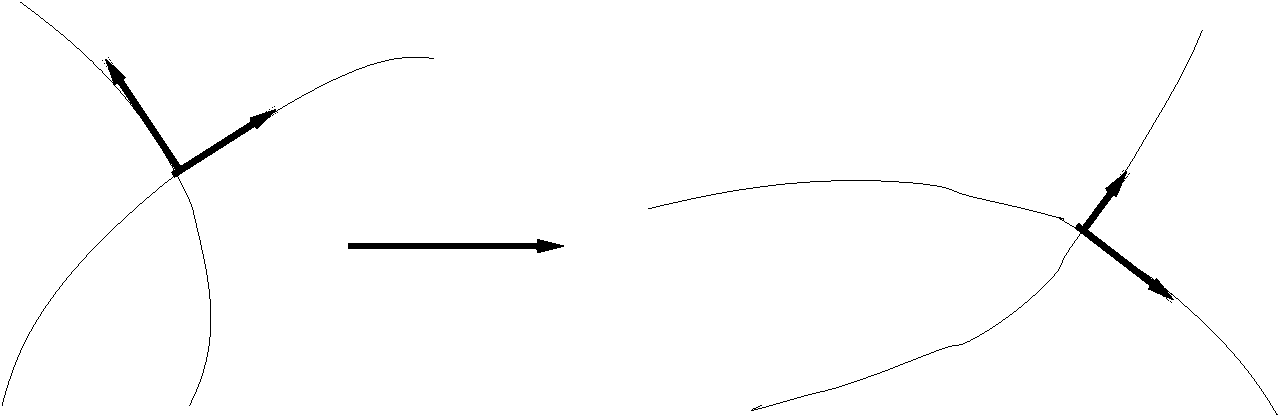
\includegraphics{images/trans_conforme.pdf}}
\caption{Transformation conforme}\label{Fi:fig2}
\end{figure}

Soit $f = P + i Q$ holomorphe dans un domaine $\Omega$. On considère
les familles de courbes définies par les équations implicites $P = t$,
$Q = u$ avec $t,u$ réels. Ces deux famille de courbes sont
orthogonales ; en effet, si l'on considère leurs images par la
transformation conforme associée à $f$, on obtient les courbes $x = t$
et $y = u$ qui sont orthogonales. Par ailleurs, les parties réelles et
imaginaires de $f$ sont des application harmoniques, i.e. solutions de
l'équation $\Delta P = 0$ (resp. $\Delta Q = 0$) avec $\Delta$
opérateur laplacien. De nombreuses relations physiques se traduisent
par une équation de la forme précédente~: c'est en particulier le cas
pour les écoulements de fluides incompressibles ou pour le potentiel
électrique. Pour résoudre ces problèmes physiques, l'utilisation de
transformations conformes associées à des application holomorphes est
souvent la méthode la plus simple. 
Soit à trouver une application $u$ de classe $C^2$ dans un domaine
$\Omega \subset \mathbb{R}^2$ de bord régulier $\partial \Omega$ telle que ~:
\[
\left \{
\begin{array}{cc}
\Delta u = 0 & \mbox{ dans } \Omega \\
u = g & \mbox{ sur } \partial \Omega \\
\end{array}
\right .
\] 
avec $g$ de classe $C^2$ sur $\partial \Omega$. S'il existe une
application holomorphe $f = P + i Q$ telle que la partie réelle $P$ (ou
la partie imaginaire $Q$) soit égale à $g$ au bord du domaine, alors celle-ci
sera solution du problème. On peut montrer que cette solution est unique en
utilisant un théorème concernant les applications harmoniques.

\begin{theorem}
Soit $f : \mathbb{R}^n \to \mathbb{R}^2$ une application de classe
$C^2$ harmonique dans un domaine $\Omega \subset \mathbb{R}^n$. Pour
toute boule ouverte $B=B(x,r)$ de $\Omega$ on a~:
\[
f(x) = \frac{1}{Vol(\partial B)} \int_{\partial B} f(s) dS
\]
\end{theorem}
\begin{proof}
$f$ harmonique vérifie $\Delta f = 0$. On a donc, en appliquant la
formule de Stokes~:
\[
\int_B \Delta f(x) dx  = 0 = \int_{\partial B} \langle grad\, f(s), n(s)
\rangle dS
\]
avec $n(s)$ normale extérieure à la sphère $\partial B$ au point $s$.
Soit mainenant l'application $h : \mathbb{R}^+ \to \mathbb{R}$ définie
par~:
\begin{align*}
h(r) &=  \frac{r^{n-1}}{Vol(\partial B(x,r))} \int_{\partial B(x,r)} f(s)  dS
\\ &= \frac{1}{Vol(\partial B(x,r))} \int_{\partial B(x,r)} f(x+r
n(\theta))  d\theta 
\end{align*}
avec $\theta$ coordonnées angulaires sur la sphère. La quantité~:
\[
\frac{r^{n-1}}{Vol(\partial B(x,r))}
\]
étant indépendante de $r$, l'application dérivée de $h$ s'écrit~:
\[
h^\prime(r) =  \frac{r^{n-1}}{Vol(\partial B(x,r))}  \int_{\partial
  B(x,r)} \langle f(x+r n(\theta)) , n(\theta) \rangle   d\theta = 0 
\]
L'application $h$ étant donc constante, le résultat cherché s'obtient
en prenant la limite pour $r \to 0$.
\end{proof} 
\begin{corollaire}
Si une application $f$ harmonique sur un domaine $\Omega$ de bord
régulier $\partial \Omega$ atteint son
maximum en un point intérieur de $\Omega$, elle est constante.  
\end{corollaire}
\begin{corollaire}
Soit $f$ application harmonique sur un domaine $\Omega$ de bord
régulier $\partial \Omega$, continue sur $\overline{\Omega}$. 
On a pour tout $x \in \Omega$~:
\[
min_{\partial \Omega} f \leq f(x) \leq max_{\partial \Omega}
\]
\end{corollaire}

Ce dernier corollaire montre que si le problème~:
\[
\left \{
\begin{array}{cc}
\Delta u = 0 & \mbox{ dans } \Omega \\
u = g & \mbox{ sur } \partial \Omega \\
\end{array}
\right .
\] 
admet deux solutions, leur différence est harmonique, de valeur 0 sur
le bord et donc nulle partout ; si une solution existe, elle est donc
unique.

Supposons que l'on connaisse une application holomorphe dont la
partie réelle est solution du problème précédent. Soit $T_h$ la
transformation conforme associée à une application holomorphe $h$. La
composée $h \circ f$ est également holomorphe, donc sa partie réelle
est harmonique et sera donc solution d'un problème du même type mais
avec un domaine différent.

\section{Fonctions définies par des séries entières}
De nombreuses applications usuelles de la variable complexe s'obtiennent comme 
sommes de séries entières. Dans la suite du cours, nous verrons que cette
situation est générale pour des applications holomorphes dans un domaine de
$\mathbb{C}$. La proposition donnée ci-dessous est un rappel de résultats déjà
vus en classes préparatoires.
\begin{fprop}\label{prop:ray_cvg}
Soit une série entière:
\[
\sum_{n \geq 0} a_n z^n
\]
Il existe un réel $r \geq 0$, appelé rayon de convergence de la série, tel que
pour tout $z \in \mathbb{C}$:
\begin{itemize}
  \item la série convergence absolument si $|z| < r$;
  \item la série est divergente si $|z|>r$;
  \item la série converge normalement sur tout disque fermé centré en 0 et de
  rayon strictement inférieur à $r$.
\end{itemize}
\end{fprop}
On dispose de plusieurs critères pour déterminer le rayon de convergence. Celui
donné ci-dessous permet également de prouver la proposition \ref{prop:ray_cvg},
mais n'est pas d'un emploi très aisé.
\begin{fprop}(critère de Hadamard)
Le rayon de convergence $r$ d'une série entière $\sum_{n \geq 0} a_n z^n$ est
donné par:
\[
r^{-1}=\limsup_{n \to +\infty} |a_n|^{\frac{1}{n}}
\]
\end{fprop}
\begin{proof}
On suppose que: 
\[
0 < \alpha = \limsup_{n \to +\infty} |a_n|^{\frac{1}{n}} <
+\infty
\]
Si $|z|<\alpha^{-1}$, il existe $\epsilon > 0$ tel que $|z|\leq
(\alpha+\epsilon)^{-1}$. Par définition de la limite sup, il existe un entier
$N$ tel que pour tout $n \geq N$:
\[
|a_n|^{\frac{1}{n}} < \alpha + \frac{\epsilon}{2}
\]
et donc, pour tout $n \geq N$:
\[
\left|a_nz^n\right|< \left(\frac{\alpha + \frac{\epsilon}{2}}{\alpha +
\epsilon}\right)^n
\]
Le terme $|a_nz^n|$ est borné par le terme général d'une série géométrique
convergente, on  en déduit l'absolue convergence de la série entière.
De même, si $|z|> \alpha^{-1}$, le même raisonnement montre que le terme
$\left|a_nz^n\right|$ est divergent. Si $\alpha = +\infty$, il existe pour tout
réel $K>0$ et tout entier $N$ un entier $n$ tel que $|a_n|>K^n$, et donc aucun
rayon de convergence non nul ne peut exister pour la série entière. Enfin, si
$\alpha = 0$, pour tout $\epsilon > 0$, il existe un entier $N$ tel que pour
tout $n \geq N$, $|a_n|<\epsilon^n$: la série converge absolument dans tout
disque ouvert centré en 0.
\end{proof}
On peut obtenir, à partir de ce critère, celui de d'Alembert:
\begin{fprop}
Soit $\sum_{n \geq 0}a_n z_n$ une série entière. Si:
\[
r^{-1} = \lim_{n \to +\infty}\frac{|a_{n+1}|}{|a_n|}
\]
existe, alors $r$ est le rayon de convergence de la série.
\end{fprop} 

C'est le critère le plus couramment employé pour déterminer le rayon de
convergence ; il n'est néanmoins pas équivalent au critère d'Hadamard.
\begin{fthm}
Soit $f$ une application définie par une série entière de rayon de
convergence $r$~:
\[
f(z) = \sum_{i \geq 0} a_i z^i
\]
$f$ est holomorphe dans le disque ouvert de centre 0 et de rayon $r$
et l'on a~:
\[
f^\prime(z) = \sum_{i \geq 1} i a_{i} z^{i-1}
\]
\end{fthm}
\begin{proof}
Soit un réel positif $r_0 < r$ et soient $z,z_0$ deux nombres complexes
de module strictement inférieur à $r_0$. Posons~:
\[
h(z) = \frac{f(z) - f(z_0)}{z-z_0}
\]
la série $h(z)$ est absolument convergente comme somme de deux séries
absolument convergentes et l'on a~:
\[
h(z) = \sum_{i \geq 1} a_i \sum_{j = 0}^{i-1} z^j z_0^{i-1-j}
\]
La série~:
\[
g(z) = \sum_{i \geq 1} i a_{i} z^{i-1}
\]
possède le même rayon de convergence que $f$ (critère de Hadamard), et sera donc
absolument convergente. 
Soient $h_n(z)$ et $g_n(z)$ les restes à partir du rang $n$ des séries
$h(z)$ et $g(z)$. On a~:
\[
|h_n(z)| \leq \sum_{i \geq 1} (n+i) |a_{n+i}| r_0^{n+i-1}
\]
la même inégalité étant vérifiée par $|g_n(z)|$. On en déduit
pour tout $\epsilon > 0$ l'existence d'un entier $n_0$ tel que pour $n
> n_0$ et pour tout $z$ de module inférieur à $z_0$, $|h_n(z)| <
\epsilon / 3$ (resp·  $|g_n(z)| < \epsilon / 3$). Par ailleurs, il
existe $\eta > 0$ tel que~:
\[
|z-z_0| < \eta \Rightarrow 
 | \sum_{i = 1}^n  i a_{i} z^{i-1} - \sum_{j = 0}^{i-1} z^j
 z_0^{i-1-j} | < \epsilon / 3 
\]
on en déduit que pour $|z-z_0| < \eta$, $|h(z) - g(z)| < \epsilon$.
\end{proof}
\begin{rem}
Par récurrence immédiate, l'application $f$ sera indéfiniment
dérivable dans son disque ouvert de convergence.
\end{rem}

\begin{fdefn}
On dit qu'une application $f : \Omega \to \mathbb{C}$, avec $\Omega$ ouvert de
$\mathbb{C}$, est analytique en $z_0 \in \Omega$ si il existe une boule ouverte
de centre $z_0$ et de rayon $r$, contenue dans $\Omega$ et une série entière
$\sum_{n \geq 0}a_n z^n$ de rayon de convergence supérieur à $r$ telles que:
\[
\forall z \in B(z_0,r), \, f(z) = \sum_{n \geq 1}a_n(z-z_0)^n
\]
On dira que $f$ est analytique dans $\Omega$ si elle est analytique en tout
point de $\Omega$.
\end{fdefn}
Le fait d'être analytique est extrêmement contraignant pour une application.
Elle doit au minimum être $C^\infty$, mais cela ne suffit pas: l'application:
\[
f \colon x \in \mathbb{R} \mapsto \left\{
\begin{array}{cc}
0 & \text{ si } x \notin ]-1,+1[ \\
\exp\left(\frac{1}{1-x^2}\right) &  \text{ si } x \in ]-1,+1[
\end{array}
\right.
\]
est $C^\infty$, mais ne peut être analytique (ses dérivées aux points $-1,+1$
sont identiquement nulles).
En revanche, tout polynôme est analytique dans $\mathbb{C}$, car égal à son
développement en série de Taylor (qui est fini). De même, l'application $z
\mapsto z^{-1}$ est analytique dans $\mathbb{C}-\{0\}$. Soit $z \neq 0$. Pour
tout $h \in \mathbb{C}$ tel que $|h|<|z|$, on peut écrire:
\[
(z+h)^{-1}=  \frac{1}{z}\frac{1}{1+\frac{h}{z}}
\]
comme $|h|<|z|$, la dernière fraction se développe en série entière et le
résultat est prouvé.

\begin{fthm}(Théorème des zéros isolés)
Soit $f$ une application analytique non identiquement nulle dans un domaine
$\Omega$. Les zéros de $f$ sont des points isolés.
\end{fthm}
\begin{proof}
La difficulté majeure du théorème vient de son caractère global. On va tout
d'abord prouver un résultat local. 
Soit $z_0 \in \Omega$ tel que $f(z_0)=0$. $f$
étant analytique, il existe un disque ouvert $B(z_0,r)$ contenu dans $\Omega$ 
et tel que dans celui-ci, $f$
admette un développement:
\[f(z)= \sum_{n \geq k}a_n (z-z_0)^n\]
avec $k$ le plus petit entier pour lequel le terme correspondant $a_k$ est non
nul (il existe si $f$ n'est pas identiquement nulle sur le disque en question).
On peut donc écrire:
\[
f(z)=(z-z_0)^p\sum_{n \geq 0}a_{n+p}(z-z_0)^n=(z-z_0)^p g(z)
\] 
L'application $g$ est continue (c'est une série entière) et ne s'annule pas en
$z_0$ où elle vaut $a_p$. Elle est donc non nulle dans tout un voisinage de
$z_0$, et donc de même pour $f$. $z_0$ est ainsi un zéro isolé. On en déduit que
si les zéros de $f$ ont un point d'accumulation, alors $f$ est identiquement
nulle au voisinage de ce point.
Le passage au global se fait par un argument
classique de connexité. Supposons que l'ensemble des zéros de $f$ dans
$\Omega$ admette un point d'accumulation $z_0$. Soit l'ensemble
\[
\mathcal{O}=\{z\in \Omega, \exists B(z,r), \, \forall u \in B(z,r), f(u)=0 \} 
\]
Il est non vide car $z_0$ y appartient. Il est ouvert car si $z \in
\mathcal{O}$, il existe une boule de centre $z$ sur laquelle $f$ s'annule
identiquement, et donc tous les points de cette boule sont dans $\mathcal{O}$.
Enfin, il est fermé, car si $(z_n)_{n\in \mathbb{N}}$ est une suite de point de
$\mathcal{O}$ admettant un point d'accumulation $w$, $f(w)=0$ par continuité et
comme $w$ est point d'accumulation d'une suite de zéros, $f$ s'annule dans un
voisinage de $w$ qui appartient donc à $\mathcal{O}$. Par connexité,
$\mathcal{O}$ est égal à $\Omega$.
\end{proof}
Ce théorème remarquable montre directement la proposition suivante
(exercice):

\begin{fprop}
Soit $f$ analytique dans un domaine $\Omega$. Le développement en série entière
de $f$ au voisinage de chaque point de $\Omega$ est unique.
\end{fprop}


On notera également que l'ensemble des zéros de $f$ dans un compact $K$ donné ne
peut être que de cardinal fini si $f$ n'est pas identiquement nulle.

\begin{fprop}(Prolongement analytique)
Soit $\Omega$ un domaine de $\mathcal{C}$ et soient $f,g$ deux applications
analytiques dans $\Omega$, coïncidant sur une partie $\mathcal{A}$ de $\Omega$.
Si $\mathcal{A}$ admet un point d'accumulation dans $\Omega$, alors $f=g$ dans
$\Omega$
\end{fprop}

Cette proposition est une conséquence directe du théorème des zéros isolés. 
\begin{rem}
On utilise fréquemment cette proposition en prenant pour $\mathcal{A}$ un ouvert
de $\Omega$.
\end{rem}
Une application définie par une série entière de rayon de convergence non nul
est analytique dans son disque ouvert de convergence. On peut facilement obtenir
l'expression de ses dérivées en tout point de ce disque. Si $f(z) = \sum_{n
\geq 0} a_n (z-z_0)^n$, on vérifie que:
\[
f^{(p)}(z) = \sum_{n \geq 0}\frac{(n+p)!}{n!}a_{n+p}(z-z_0)^n,\;
f^{(p)}(z_0)=p!a_p
\]
 Un grand nombre d'applications réelles usuelles s'étendent au cas complexe par
 prolongement analytique. Des exemples importants sont donnés dans la section
 suivante.
\subsection{Exponentielle}
C'est l'application holomorphe dans $\mathbb{C}$, notée $e^z$ et
définie par la série entière de rayon de convergence infini~:
\[
e^z = \sum_{i \geq 0} \frac{z^i}{i!}
\]
L'application dérivée de l'exponentielle est elle-même. 
Pour $z_1,z_2 \in \mathbb{C}$, on a~:
\begin{align*}
e^{z_1+z_2} & = \sum_{i \geq 0} \frac{(z_1+z_2)^i}{i!} = 
\sum_{i \geq 0} \frac{\sum_{j=0}^i C_i^j z_1^j z_2^{i-j}}{i!} \\
& = \sum_{i \geq 0} \sum_{j=0}^i \frac{z_1^j}{j!}
\frac{z_2^{i-j}}{(i-j)!} = e^{z_1} e^{z_2}
\end{align*}
On vérifiera aisément que pour $z = x + iy$~:
\[
e^z = e^x (cos y + i sin y)
\]
et que~:
\[
e^{-z} = \frac{1}{e^z}
\]
\begin{exercice}
Soit la série entière:
\[
f \colon z \mapsto \sum_{n >0}(-1)^{n-1}\frac{(z-1)^n}{n}
\]
\begin{itemize}
  \item Déterminer son rayon de convergence;
  \item Montrer que pour tout réel $x \in ]0,2[$, $f(x)=\log(x)$;
  \item En déduire que $f$ est l'unique application analytique prolongeant le
  logarithme réel sur le disque ouvert $B(1,1)$;
  \item Vérifier que sur $B(1,1)$, on a $\exp \circ f = Id$.
\end{itemize}
\end{exercice}

\subsection{Fonctions hyperboliques}
Elles se définissent à partir de l'exponentielle comme dans le cas
réel.
\begin{align*}
ch z &= \frac{e^z + e^{-z}}{2} \\
sh z &= \frac{e^z - e^{-z}}{2} \\
th z &= \frac{e^{2z} - 1}{e^{2z} + 1} \\
\end{align*}
\begin{itemize}
\item $ch, sh$ sont holomorphes dans $\mathbb{C}$ 
\item $th$ est holomorphe dans
$\mathbb{C} - \left \{ i \left (n+\frac{1}{2})\pi \right ) , \, n \in
  \mathbb{Z} \right \}$
\end{itemize} 
les applications dérivées des fonctions hyperboliques sont~:
\[
ch^\prime z = sh z \, , \, sh^\prime z = ch z \, , \, 
th^\prime z = \frac{1}{ch^2 z}
\]
\subsection{Fonctions circulaires}
Elles sont définies par~:
\begin{align*}
cos z &= \frac{e^{iz} + e^{-iz}}{2} \\
sin z &= \frac{e^{iz}z - e^{-iz}}{2i} \\
tan z &= \frac{1}{i}\frac{e^{2iz} - 1}{e^{2iz} + 1} \\
\end{align*}
\begin{itemize}
\item $cos,sin$ sont holomorphes dans $\mathbb{C}$
\item $tan$ est holomorphe
dans $\mathbb{C} - \left \{ \left (n+\frac{1}{2})\pi \right ) , \, n \in
  \mathbb{Z} \right \}$
\end{itemize}
Les applications dérivées sont~:
\[
cos^\prime z = -sin z \, , \, sin^\prime z = cos z \, , \, 
tan^\prime z = \frac{1}{cos^2 z}
\]
\subsection{Fonctions spéciales}
De très nombreuses fonctions utilisées en physique ou obtenues comme solutions d'équations différentielles s'expriment facilement sous la forme d'une série entière. L'exercice ci-dessous définit la fonction de Bessel.
\begin{exercice}
Soit $\nu$ un entier. L'équation de Bessel d'ordre $\nu$ est:
\begin{equation}\label{eq:bessel}
z^2 \frac{d^2f}{dz^2} + z \frac{df}{dz} + \left(z^2-\nu^2\right)f = 0
\end{equation}
\begin{itemize}
\item Soit $f$ une solution de (\ref{eq:bessel}) que l'on suppose développable en série entière au voisinage de $0$. En écrivant son développement sous la forme:
\[
f \colon z \mapsto \sum_{n=0}^{+\infty} a_n x^{n+k}
\]
où $k$ est un entier, on a les relations:
\begin{eqnarray}
a_0 \left(k^2 - \nu^2\right) = 0 \\
a_1 \left(((k+1)^2 - \nu^2\right) = 0 \\
a_n \left((k+n)^2 - \nu^2\right) + a_{n-2} = 0, \, n \geq 2
\end{eqnarray}
\item En posant $k = \nu$, montrer que si $f$ solution de (\ref{eq:bessel}) est développable en série entière au voisinage de $0$ et vérifie $a_0=1/(2^\nu \nu!)$, son développement est:
\[
f \colon z \mapsto \left(\frac{z}{2}\right)^\nu \sum_{n=0}^{+\infty} \frac{(-1)^n}{n!(n+\nu)!}\left(\frac{z}{2}\right)^{2n}
\]
\item En utilisant le critère de Hadamard et la formule de Stirling:
\[
n! \sim_{+\infty} \sqrt{2 \pi n}\left(\frac{n}{e}\right)^n
\]
montrer que le rayon de convergence de la série est infini.
\end{itemize}
\end{exercice}
\subsection{Calcul numérique}
Le développement en série entière est un moyen numérique simple d'évaluer une fonction en un point. Nous verrons plus loin que toutes les applications
holomorphes dans un domaine y sont analytiques, montrant ainsi qu'au moins en principe, il est toujours possible de les calculer de façon approchée. C'est un résultat remarquable et sans équivalent dans $\R$, à tel point qu'il est parfois plus simple de travailler dans $\C$ même pour des applications réelles. Le code qui est proposé ici va évaluer la fonction d'erreur dans le plan complexe. On la rencontre très souvent dans les calculs faisant intervenir la loi normale. Elle a pour expression, dans le cas d'un argument réel:
\[
\erf{x} = \frac{2}{\sqrt{\pi}} \int_0^x e^{-t^2}dt
\]
Son extension complexe peut aussi s'obtenir comme une intégrale de chemin, que nous verrons dans les chapitres suivants, mais nous utiliserons son expression en série entière qui est:
\[
\erf{z} =  \frac{2}{\sqrt{\pi}} \sum_{n=0}^\infty \left(-1\right)^n \frac{z^{2n+1}}{n!\left(2n+1\right)}
\]
\begin{itemize}
\item A partir du développement en série entière de $\exp$, pouvez-vous retrouver celui de $\erf$ ?
\item Quel est le rayon de convergence de la série entière donnant $\erf$ ?
\item Donner une borne supérieure de l'erreur commise en arrêtant la sommation de la série au rang $N$ et en supposant
le terme général décroissant. Vérifier que cette dernière hypothèse est satisfaite si le rang de la somme partielle est supérieur à $|z|^2$.
\end{itemize}
Le code Python donné ci-dessous calcule $\erf$ à partir de la série entière et compare la valeur obtenue à celle de la fonction
de bibliothèque $\erf$.
\begin{verbatim}
# -*- coding: utf8 -*-
import math

# Calcul de la fonction d'erreur par une série entière. 
# La tolérance sur le résultat est passé en second paramètre.
# z : complexe
# tol: réel positif
# return: complexe
def erf_serie(z,tol):
    t = z # produit partiel permettant le calcul du 
    # terme général de la série
    s = t # somme partielle
    tol = abs(tol) # in case of a negative tolerance
    err = abs(t) # estimation de l''erreur
    i = 1 # compteur du nombre d'itérations
    min_i = int(abs(z) * abs(z)) # nombre d'itérations
    # assurant la décroissance du terme général
    while err > tol or i < min_i:
        t = - t * z * z / i
        term = t / ( 2.0 * i + 1.0)
        s = s + term
        i = i + 1 
        err = abs(term)
    return 2 * s / math.sqrt(math.pi)

print(erf_serie(complex(0.5,0.0),1e-8), math.erf(0.5))
print(erf_serie(complex(1.0,0.0),1e-8), math.erf(1))
print(erf_serie(complex(3.0, 0.0),1e-8), math.erf(3))
print(erf_serie(complex(5.0, 0.0),1e-8), math.erf(5))
print(erf_serie(complex(10.0, 0.0),1e-8), math.erf(10))
\end{verbatim} 

 L'adéquation est bonne pour les faibles valeurs mais ne l'est pas à partir de 5. On peut essayer de comprendre ce qui se passe en affichant les valeurs intermédiaires du calcul pour $z=10$, à l'aide du code suivant:
 \begin{verbatim}
 # -*- coding: utf8 -*-
 import math
 
 # Calcul de la fonction d'erreur par une série entière. 
 # La tolérance sur le résultat est passé en second paramètre.
 # z : complexe
 # tol: réel positif
 # return: complexe
 def erf_serie(z,tol):
     t = z # produit partiel permettant le calcul du 
     # terme général de la série
     s = t # somme partielle
     tol = abs(tol) # in case of a negative tolerance
     err = abs(t) # estimation de l''erreur
     i = 1 # compteur du nombre d'itérations
     min_i = int(abs(z) * abs(z)) # nombre d'itérations
     # assurant la décroissance du terme général
     while err > tol or i < min_i:
         t = - t * z * z / i
         print(i,t)
         term = t / ( 2.0 * i + 1.0)
         s = s + term
         i = i + 1 
         err = abs(term)
     return 2 * s / math.sqrt(math.pi)
 
 # print(erf_serie(complex(0.5,0.0),1e-8), math.erf(0.5))
 # print(erf_serie(complex(1.0,0.0),1e-8), math.erf(1))
 # print(erf_serie(complex(3.0, 0.0),1e-8), math.erf(3))
 # print(erf_serie(complex(5.0, 0.0),1e-8), math.erf(5))
 print(erf_serie(complex(10.0, 0.0),1e-8), math.erf(10))
 \end{verbatim}
 Au voisinage de la centième itération pour $z=10$, on trouve:
 \begin{verbatim}
 (97, (-1.0395792815393291e+43+0j))
 (98, (1.0607951852442134e+43+0j))
 (99, (-1.0715102881254682e+43+0j))
 (100, (1.0715102881254682e+43+0j))
 (101, (-1.0609012753717507e+43+0j))
 (102, (1.0400992895801476e+43+0j))
 (103, (-1.0098051355147064e+43+0j))
 \end{verbatim}
 montrant que l'on passe par de très grandes valeurs avant de décroître:
 \begin{verbatim}
 (280, (5.962219395344518e-05+0j))
 (281, (-2.1217862616884407e-05+0j))
 (282, (7.5240647577604285e-06+0j))
 (283, (-2.6586801264171127e-06+0j))
 \end{verbatim}
 Ceci explique l'erreur considérable commise en calculant par la série entière: pour conserver la précision cible de $10^{-8}$, sur les termes au voisinage de l'itération 100, il faudrait environ 50 chiffes significatifs, alors que l'arithmétique flottante de python (et de presque tous les langages !) n'en offre que 15 (type dit "double précision"). 
 \begin{danger}
 Il est très important de bien vérifier à chaque étape d'un calcul l'ordre de grandeur des termes. La garantie de convergence théorique ne présuppose en rien du bon fonctionnement d'un algorithme implanté sur une machine dont l'arithmétique est de précision finie.
 \end{danger}
 
 En conclusion, l'évaluation d'une fonction analytique à l'aide de sa série entière n'est vraiment intéressante qu'au voisinage du point de référence, 0 le plus souvent. Ailleurs, on utilisera des propriétés particulières de la fonction (comme la périodicité)pour tenter de s'y ramener.
\chapter{Intégration des applications d'une variable complexe}
\section{Intégration le long d'un chemin}
On rappelle qu'une forme différentielle $\omega$ de degré 1, définie sur un
domaine $U$ de $\mathbb{C}$ et à valeurs dans $\mathbb{C}$, admet une écriture:
\[
\omega=\alpha dz + \beta d\overline{z}
\]
Une telle forme peut s'intégrer le
long d'un chemin de classe $C^1$ par morceaux $\gamma \colon [0,1] \to U$ et, conformément aux résultats du chapitre 8, on a:
\[
\int_{\gamma} \omega = \int_{[0,1]}\left(\alpha \circ \gamma\right)(t)
\gamma^\prime(t)dt + \int_{[0,1]}\left(\beta \circ \gamma\right)(t)
\overline{\gamma^\prime}(t)dt
\]
Soit une application continue $f \colon U \to \mathbb{C}$, on peut lui associer
de façon canonique deux formes différentielles de degré 1, $fdz$ et 
$f d\overline{z}$. On définira:
\[
\int_{\gamma}f dz = \int_{[0,1]}f\left(\gamma(t)\right)\gamma^\prime(t)dt
\]
et 
\[
\int_{\gamma}f d\overline{z} =
\int_{[0,1]}f\left(\gamma(t)\right)\overline{\gamma^\prime}(t)dt
\]

La première expression est appelée intégrale de $f$ le long du chemin $\gamma$.
 Cette formule permet le calcul de nombreuses
intégrales le long de chemins de classe $C^1$. On va par exemple rechercher la
valeur de ~:
\[
\int_{\gamma} \frac{dz}{z}
\]
où $\gamma$ est le chemin $[0, 1] \to \mathbb{C}$ tel que
$\gamma(\theta) = \exp(i 2 \pi \theta)$. L'image de ce chemin est le cercle
unité de $\mathbb{C}$. Il est parcouru une seule fois dans le sens
trigonométrique. On a~: $\gamma^\prime(2 \pi \theta) = i 2 \pi \exp(i 2
\pi \theta)$ et~:
\[
\int_{\gamma} \frac{dz}{z} =  \int_0^1 \exp(-i 2 \pi \theta) (i 2 \pi \exp(i
2 \pi \theta)) d \theta = i 2 \pi 
\]

On peut évaluer l'intégrale de la même application relativement à
$d\overline{z}$:

\begin{align*}
\int_{\gamma} \frac{d\overline{z}}{z} & =  \int_0^1 \exp(-i 2 \pi \theta) (-i 2
\pi \exp(-i 2 \pi \theta)) d \theta  \\
&= -i 2 \pi \int_0^1 \exp(-i4 \pi \theta)
d \theta = 0
\end{align*}



\begin{fprop}
Soit $\gamma : \, [0,1] \to \mathbb{C}$ un chemin de classe $C^1$ par morceaux et soit
$f$ une application  intégrable le long de $\gamma$. Alors~:
\[
\left|\int_{\gamma} f(z) dz\right | \leq \int_{[0,1]} \left |f(\gamma(t)) \right | \left |\gamma^\prime(t) \right | dt
\]
\end{fprop}
On peut obtenir facilement ce résultat en utilisant les sommes de Riemann-Stieltjes.
Cette majoration est utilisée pour obtenir un résultat très utile en
pratique~: le lemme de Jordan.

\begin{fprop}(Lemme de Jordan)\label{prop:jordan}
Soit $\gamma_r$ le chemin formé d'un arc de cercle de rayon $r$, de centre $z_0$ parcouru
 dans le sens trigonométrique, d'angle initial $\alpha_0$ et d'angle final
 $\alpha_1$. Soit $f$ une application continue sur $\gamma_r$ pour
 tout $r>0$. Si la borne supérieure de l'application $|(z-z_0)f(z)|$ tend vers 0 lorsque $r$ 
 tend vers $0$ (resp. $+\infty$), alors~:
\[
\lim_{r \to 0^+ (resp. +\infty)} \int_{\gamma_r} f(z) dz = 0
\]
\end{fprop}
\begin{proof}
Pour $r$ fixé, le chemin $\gamma_r$ s'exprime par:
\[
\gamma_r \colon t \in [0,1] \mapsto z_0 + r e^{i \left(\alpha_0 +
t (\alpha_1 - \alpha_0)\right)}
\]
On a donc:
\[
\left|\int_{\gamma_r} f(z) dz\right| \leq (\alpha_1-\alpha_0) \int_0^1
|f(\gamma_r(t))|r dt 
\]
On remarque par ailleurs que $|(z-z_0)f(z)|=r|f(z)|$ pour $z$ appartenant à
l'image de $\gamma_r$. La conclusion du théorème s'obtient alors directement.
\end{proof}
\section{Formules de Cauchy}
Les résultats de cette section sont fondamentaux pour la suite. Ils vont
permettre en particulier d'établir que tout application holomorphe dans un
domaine y est en fait analytique.
\begin{fdefn}
Un chemin $\gamma \colon [0,1] \to \C$ de classe $C^1$ est dit régulier si $\gamma^\prime(t) \neq 0, \, t \in ]0,1[$. Un chemin de classe $C^1$ par morceaux est régulier s'il l'est sur chaque sous-intervalle où il est continûment différentiable. 
\end{fdefn}
\begin{fthm}(Stokes complexe)\label{thm:stokes_complexe} Soit $\Omega$ un domaine de $\mathbb{C}$
admettant pour bord $\partial \Omega$ un lacet simple régulier de
classe $C^1$ par morceaux. Soit $f : \mathbb{C} \to \mathbb{C}$
application de classe $C^1$ dans $\Omega$ (au sens $\mathbb{R}^2$) et continue
sur $\Omega \cup \partial \Omega$. Alors~:
\[
\int_{\partial \Omega} f(z) dz = - \int_{\Omega} \frac{\partial
f}{\partial \overline{z}} dz d\overline{z}
\]
où l'intégrale en partie droite est faite en considérant $z,\overline{z}$ comme des variables indépendantes.
\end{fthm}

La preuve de ce théorème, qui est essentiellement une application de la formule
de Stokes, va être détaillée à l'aide de deux lemmes fondamentaux.
\begin{lemme}
Soit $\gamma \colon [0,1] \to \mathbb{C}$ un lacet simple régulier de
classe $C^1$. Il existe un nombre fini de couples $(U_i, \theta_i)_{i=1\dots N}$ avec $U_i$
ouvert de $\mathbb{R}^2$ et $\theta_i$ difféomorphisme de classe $C^1$ de $U_i$
dans $\mathbb{R}^2$ vérifiant les assertions suivantes:
\begin{enumerate}
  \item la famille $(U_i)_{i=1\dots N}$ forme un recouvrement ouvert de l'image
  de $\gamma$.
  \item l'image de $\gamma([0,1])\cap U_i$ par $\theta_i$ est un segment de
  l'axe des abscisses.
\end{enumerate}
\end{lemme}
\begin{proof}
Soit $\gamma(t_0)$ un point de l'image de $\gamma$. On a, par régularité de
$\gamma$,  $\gamma^\prime(t_0) \neq 0$. 
Soit l'application:
\[
(t,s) \to \gamma(t) + s v
\]
définie pour $t$ assez proche de $t_0$. Sa dérivée en $(t_0,0)$ a pour matrice
jacobienne:
\[
\left(
\gamma^\prime(t_0), v
\right)
\]
qui est inversible. Le théorème d'inversion locale montre alors qu'il existe un
voisinage ouvert $U_{t_0}$ contenant $\gamma(t_0)$ et un difféomorphisme
$\theta_{t_0}$ de classe $C^1$ défini sur $U$ tel que $\theta_{t_0}(U_{t_0})$
contienne un pavé $]t_0-\epsilon, t_0+\epsilon[ \times ]-\eta, \eta[$ avec
$\epsilon >0, \eta > 0$. Pour tout $t \in ]t_0-\epsilon, t_0+\epsilon[$, on a
$\theta^{-1}(t,0)=\gamma(t)$ par construction. En revanche, il peut exister des
couples $(t,s), s \neq 0$ tels que $\theta^{-1}(t,s)=\gamma(\tilde{t})$, et dans
ce cas $\tilde{t} \notin ]t_0-\epsilon, t_0+\epsilon[$. Soit $\Delta$ l'ensemble
de ces couples. Il existe un pavé $]t_0-\epsilon_1, t_0+\epsilon_1[ \times
]-\eta_1, \eta_1[$ avec $\epsilon_1 > 0$, $\eta_1 > 0$ et ne rencontrant pas
$\Delta$. Supposons cette propriété fausse. Il existe alors une suite de points
$(t_i,s_i)$, $s_i \neq 0$ de limite $(t_0,0)$. Pour tout entier $i$, soit
$\tilde{t}_i$ un point tel que $\gamma(\tilde{t}_i)=\theta^{-1}(t_i,s_i)$. La
suite $\tilde{t}_i, i\in \mathbb{N}$ appartient au compact $[0,1]$ et admet un point
d'accumulation $\tilde{t} \notin ]t_0-\epsilon, t_0+\epsilon[$. Par continuité
de $\gamma$, $\gamma(\tilde{t})=\gamma(t_0)$, ce qui contredit le fait que
$\gamma$ soit un homéomorphisme. On peut donc choisir l'ouvert $U_{t_0}$ de
telle sorte que l'image de $\gamma([0,1]\cap U_{t_0})$ soit un segment de l'axe
des abscisses.
La preuve du lemme se déduit directement de cette propriéte et de la compacité
de $\gamma([0,1])$: La famille $(U_t)$ forme un recouvrement ouvert de
$\gamma([0,1])$, on peut donc en extraire une sous-famille finie qui répond aux
conditions du lemme.
\end{proof}
% Ce lemme permet d'obtenir une forme affaiblie de théorème de Jordan.
%Pour ce faire, on va montrer qu'il existe une partition de $\mathbb{R}^2$ en points
%d'indice nul et points d'indice égal à $\pm 1$ (le signe étant toujours le
%même). On se donne une courbe de Jordan régulière $\gamma$ de classe $C^1$.
%Soit $x \in \mathbb{R}^2$ et soit $v$ un vecteur quelconque non nul. Si la
%demi-droite de sommet $x$ et de vecteur directeur $v$ a une intersection vide
%avec l'image de $\gamma$, l'indice de $x$ est 0: en effet, les points de la
%demi-droite suffisamment loin de l'origine sont d'indice nul et par continuité
%de l'indice, $x$ doit aussi avoir un indice nul. Sinon, il existe un nombre fini
%de domaines $u_i$ dans lesquels une intersection a lieu. En modifiant
%éventuellement $v$, il est toujours possible de supposer que les intersections 
%sont réduites à un point. On raisonne de la façon suivante: en partant d'un
%point de la demi-droite d'indice 0, on chemine vers $x$ (i.e. selon la
%direction $-v$) jusqu'au premier point d'intersection $x_1$. Après
%transformation par le difféomorphisme $\theta_1$ correspondant à l'ouvert $U_1$
%contenant $x_1$, on compare le sens de parcours du chemin et celui du parcours
%de la demi-droite. Si les deux vecteurs sont en sens direct, on augmente d'une
%unité l'indice des points placés après l'intersection, sinon on le diminue d'une
%unité. Cette procédure est schématisée figure \ref{fig:jordan} et s'explique très
%facilement: dans un cas le chemin s'enroule en sens trigonométrique autour des points situés
%après l'intersection, l'indice doit donc augmenter, dans l'autre cas il doit
%diminuer. On répète l'opération de proche en proche jusqu'à atteindre le point
%$x$. Trois cas uniquement peuvent se présenter: l'index de $x$ vaut $0$
% s'il y a eu un nombre pair d'intersections, et $+1$ ou $-1$ s'il y en a eu un
% nombre impair (les signes aux intersections doivent en effet s'alterner, sans
% quoi on ne pourrait avoir un lacet simple). Pour la même raison, il n'est pas
% possible d'avoir à la fois des points d'indice $+1$ et $-1$. L'ensemble des
% points d'indice non nul forme un domaine de $\mathbb{R}^2$, de bord l'image de
% $\gamma$ et ceux d'indice nul un domaine non borné, ce qui est précisément la
% conclusion du théorème de Jordan.
% \begin{figure}[ht]
%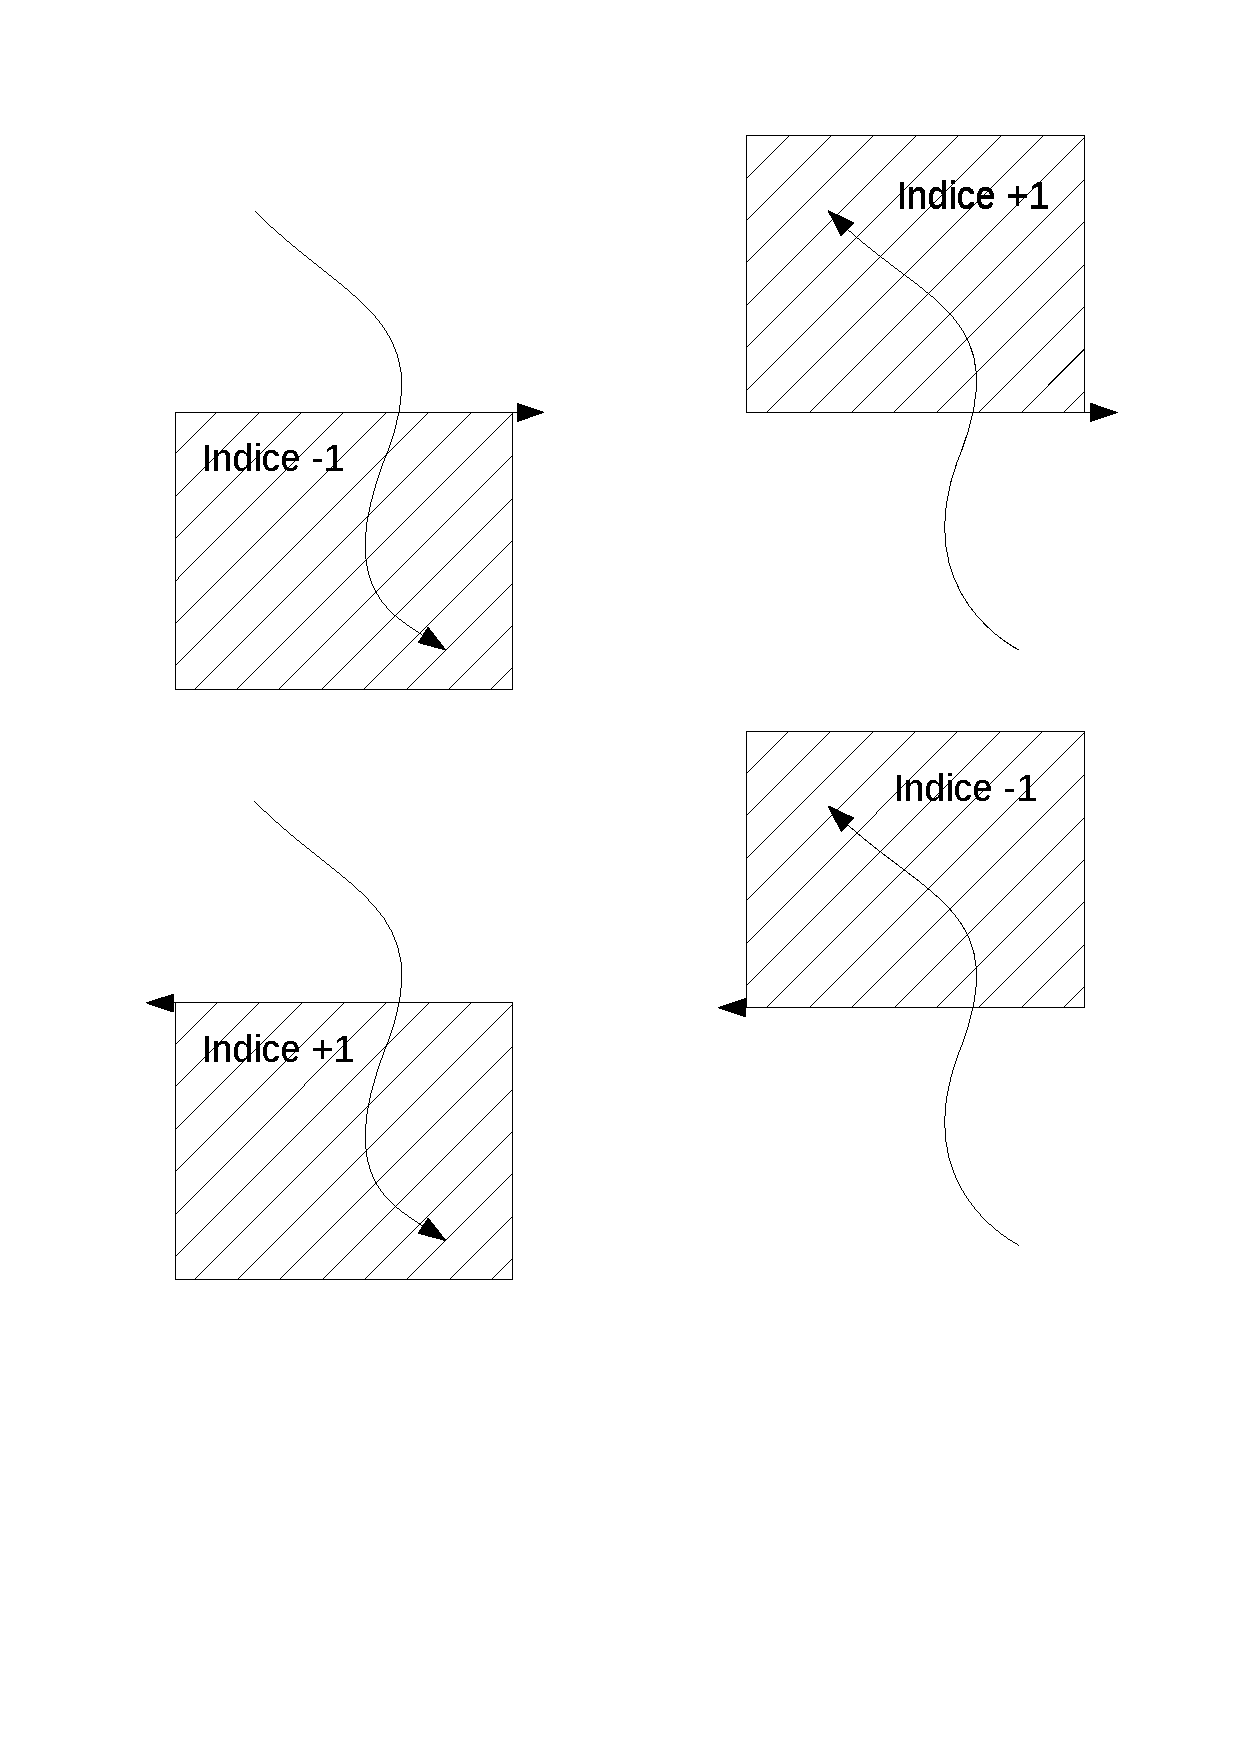
\includegraphics[scale=0.3]{images/jordan.pdf}
%\caption{Franchissement d'un lacet}\label{fig:jordan}
%\end{figure}
%On peut utiliser de façon pratique le procédé précédent pour déterminer
%rapidement si un point appartient au domaine intérieur à une courbe de Jordan;
%c'est un algorithme que l'on rencontre couramment dans les logiciels de dessin
%ou de conception assistée par ordinateur, en concurrence avec celui basé sur un
%calcul de l'indice par intégration que nous verrons plus loin.
%
%On notera la latitude laissée dans le choix de la direction $v$ utilisée dans
%la preuve du lemme. En particulier, si $U$ est le domaine intérieur à $\gamma$,
%on pourra toujours choisir les difféomorphismes $\theta_i$ de telle façon 
%que l'image de  $U \cap U_i$ par $\theta_i^{-1}$ soit contenue dans le
%demi-espace $\mathbb{R}\times \mathbb{R}^+$. La portion de courbe $\gamma$,
%forme un segment de l'axe des abscisses et sera parcouru soit dans le sens des 
%abscisses croissantes, soit dans le sens des abscisses décroissantes. 
%Dans le premier cas, l'indice devra être +1 pour les points intérieurs
%et donc -1 dans le second cas. 
%L'indice étant constant, on en déduit que le sens de parcours sera le même dans
%tous les morceaux obtenus par applications des $\theta_i^{-1}$. On dira que $\gamma$ est
%orientée en sens positif si l'indice des points intérieurs est +1, en sens
%négatif s'il vaut -1. L'orientation d'une courbe de Jordan est toujours
%possible, mais ceci ne reste plus vrai en dimension supérieure, même pour des
%surfaces très régulières: des exemples de surfaces $C^\infty$ non orientables
%peuvent facilement être obtenus.

Le lemme peut être étendu à un chemin de classe $C^1$ par morceaux:
\begin{lemme}
Soit $\gamma$ un lacet simple régulier de classe $C^1$ par morceaux. Il
existe pour tout point $t_0$ où la dérivée de $\gamma$ est discontinue un voisinage ouvert
$U$ de $\gamma(t_0)$ dans $\mathbb{C}$,un voisinage ouvert $V$ de $(t_0,0)$ dans
$\mathbb{R}^2$ et un difféomorphisme $\theta$ de classe $C^1$ de $U$ dans $V$
tels que l'image de $\gamma([0,1]) \cap U$ soit la réunion d'un segment du
demi-axe des abscisses négatif et d'un segment de l'axe du demi-axe des
ordonnées positif.
\end{lemme}
\begin{proof}
La démonstration est semblable à celle du lemme précédent. On notera $\gamma^-$
(resp. $\gamma^+$) la portion de l'image du lacet $\gamma$ formée des points
$\gamma(t), t < t_0$ (resp. $\gamma(t),t > t_0$). On peut compléter $\gamma^+,
\gamma^-$ dans un voisinage de $t_0$ de telle façon que le chemin ainsi obtenu
soit de classe $C^1$:on peut par exemple prolonger par un segment de droite de
vecteur directeur la limite à gauche (resp. à droite) de la dérivée de $\gamma$
en $t_0$. On continuera à désigner $\gamma^+, \gamma^-$ les chemins ainsi
prolongés. Dans un voisinage de $(t_0,t_0)$, on définit l'application:
\[
(t,s) \mapsto \gamma(t) + \gamma(s) - \gamma(t_0)
\]
Sa matrice Jacobienne en $(t_0,t_0)$ est:
\[
\left(
\gamma^\prime(t_0^-), \gamma^\prime(t_0^+) 
\right )
\]
qui est de rang maximal si $t_0$ est un point de discontinuité de la dérivée. 
Le théorème d'inversion locale permet alors de conclure.
\end{proof}
 Il est maintenant possible de procéder à la preuve du
théorème.
\begin{proof}
On posera $f = P + i Q$. Soit $U$ le domaine intérieur bordé par le lacet simple régulier $\partial \Omega$. Soient enfin $U_i, i=1\dots N$ les ouverts
donnés par le premier ou le second lemme selon que l'on est ou non au voisinage
d'un point de discontinuité de la dérivée. Le recouvrement ouvert $U \cup
\bigcup_{i=1}^N U_i$ admet une partition de l'unité $\alpha_i, i=0\dots N$ subordonnée 
(on note $\alpha_0$ le terme associé à $U$). Considérons les formes différentielles continues de
degré 1:
\[
\omega_1 = P dx - Q dy, \quad \omega_2= Qdx + Pdy 
\]
on a:
\[
d\omega_1 = -\left(\frac{\partial P}{\partial y}+\frac{\partial Q}{\partial
x}\right )dx \wedge dy
\]
et
\[
d\omega_2 = \left(\frac{\partial P}{\partial x}-\frac{\partial Q}{\partial
y}\right )dx \wedge dy
\]
L'intégrale:
\[
\int_{U} \alpha_0 d\omega_1 = - \int_{U}\alpha_0(x,y) \left(\frac{\partial
P}{\partial y}(x,y)+\frac{\partial Q}{\partial x}(x,y)\right )dxdy
\]
vaut $0$, le support de $\alpha_0$ se trouvant dans $U$. La même propriété
est vraie pour $d\omega_2$. Soit maintenant un des ouverts $U_i, i=1\dots N$ et
$\theta_i^{-1}$ le difféomorphisme de classe $C^1$ associé (on choisit de
travailler avec $\theta_i^{-1}$ pour simplifier les notations). On remarquera
tout d'abord (le vérifier !) que $\theta_i^*\left(\alpha_i d \omega_1\right) =
\alpha_i\circ \theta_i d \theta_i^* \omega_1$. On a donc:
\[
\int_{U_i} \alpha_i d \omega_1  = \int_{\theta_i(U_i)} \alpha_i\circ \theta_i d
\theta_i^* \omega_1
\]
La formule de Stokes élémentaire (qui s’étend très facilement dans le
cas des images d'ouverts contenant une singularité) appliquée à l'ouvert
$\theta_i(U_i)$ montre que l'intégrale précédente vaut $\int_{\theta_i(\gamma[0,1]\cap U_i)} 
\left (\alpha_i \circ \theta_i\right) \theta_i^*(\omega_i)$ qui s'identifie à
l'intégrale de la partie réelle de $f$ sur la portion de chemin appartenant à
$U_i$. Un raisonnement similaire peut se faire sur $\omega_2$: on en déduit le
théorème par sommation sur les $U_i$.
\end{proof}
Ce théorème permet d'obtenir un corollaire très simple, mais très utile: si $f$
vérifie les hypothèses précédente et est holomorphe, alors l'intégrale le long
de $\partial \Omega$ vaut 0. 
La formule \ref{thm:stokes_complexe} n'est pas valable pour des domaines présentant des trous, tels celui de la figure \ref{fig:domaine_trois_connexe}.
\begin{figure}[ht]
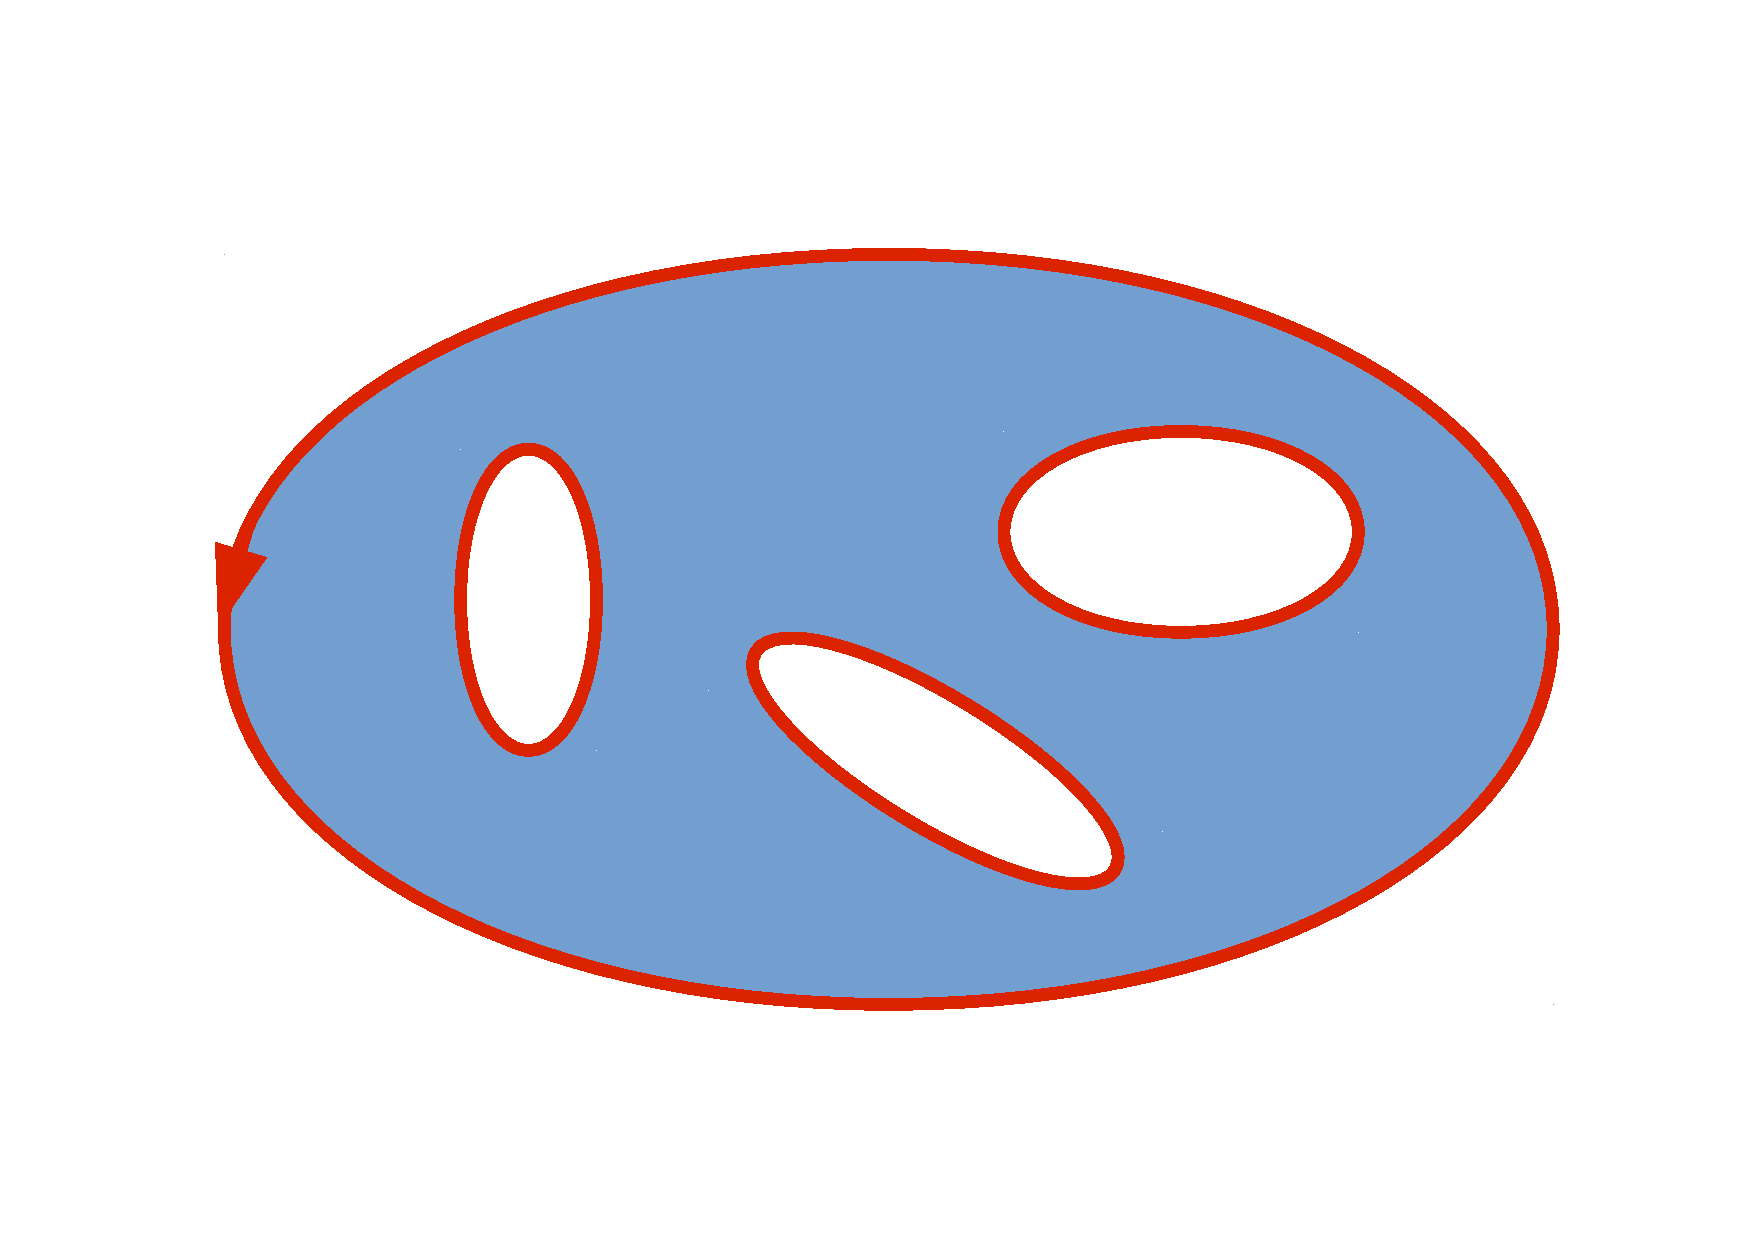
\includegraphics[scale=0.3]{images/domaine_trois_connexe.pdf}
\caption{Domaine 3-connexe}\label{fig:domaine_trois_connexe}
\end{figure}
Si le bord est formé d'une union disjointe de lacets simples réguliers de classe $C^1$, on peut néanmoins continuer à appliquer le théorème en prenant garde à orienter en sens direct le contour extérieur et en sens rétrograde les lacets internes. 

Le théorème qui vient d'être énoncé permet de calculer des intégrales de la
variable réelle difficiles à obtenir de façon directe. L'exercice suivant permet 
d'évaluer les intégrales de Fresnel, que l'on rencontre assez fréquemment en
physique (ces intégrales sont issues d'un problème d'optique).
\begin{exercice}
Soit l'application $f \colon z \mapsto \exp\left(i z^2\right)$. 
\begin{itemize}
  \item Montrer que $f$ est holomorphe sur $\mathbb{C}$ et vérifier que sa
  dérivée est continue.
  \item Pour tout réel $r > 0$, le contour $\gamma_r$ est défini selon la figure
  \ref{fig:contour2}. Donner la valeur de l'intégrale:
  \[
  \int_{\gamma_r} f(z) dz
  \]
  \item Écrire cette intégrale sous la forme d'une somme de trois
  intégrales de chemin et montrer que l'intégrale correspondant à l'arc de
  cercle tend vers 0 lorsque $r \to +\infty$.
  \item En déduire les valeurs des intégrales généralisées suivantes, dites
  intégrales de Fresnel:
  \[
  \lim_{r \to +\infty} \int_{[-r,r]} \cos(x^2) dx, \quad  \lim_{r \to +\infty}
  \int_{[-r,r]} \sin(x^2) dx
  \]
\end{itemize}
\end{exercice}
 \begin{figure}[ht]
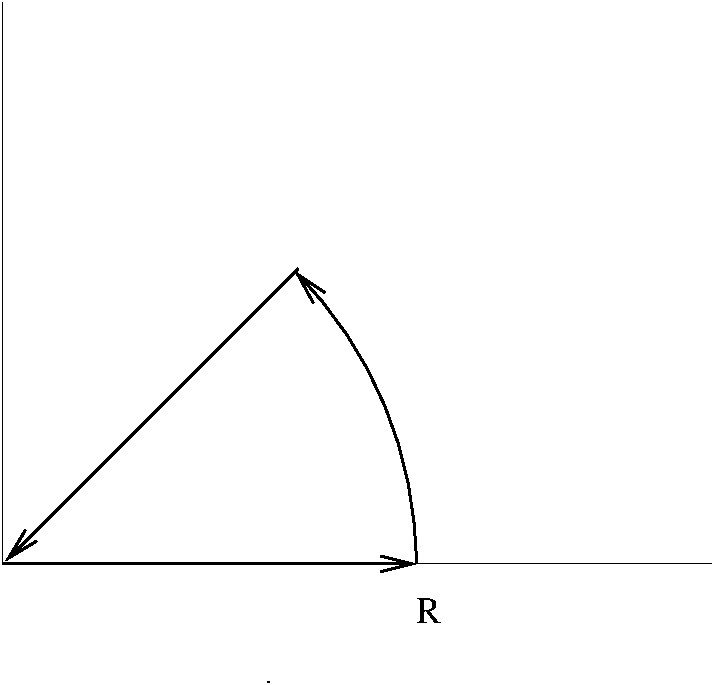
\includegraphics[scale=0.3]{images/contour_fresnel.pdf}
\caption{Contour $\gamma_r$}\label{fig:contour2}
\end{figure}
On utilise fréquemment les techniques d'intégration dans le plan complexe pour
obtenir des transformées de Fourier. L'exercice suivant calcule la transformée
de Fourier d'une gaussienne, qui a déjà été obtenue précédemment à l'aide d'une
équation différentielle. 
\begin{exercice}
Soit $f \colon z \in \mathbb{C} \mapsto \exp(-z^2)$.
\begin{itemize}
  \item Montrer que $f$ est holomorphe dans $\mathbb{C}$, de dérivée continue.
  \item En utilisant le contour $\gamma_r$ donné figure , déterminer, pour
  $\omega \in \mathbb{R}$ fixé, la valeur de l'intégrale:
  \[
  \int_{\gamma_r} \exp(-z^2)dz
  \]
  \item En faisant tendre $r$ vers $+\infty$ et en faisant un raisonnement
  similaire à celui de l'exercice précédent, déterminer la transformée de
  Fourier de l'application $x \mapsto \exp(-x^2)$.
\end{itemize}
\end{exercice}
 \begin{figure}[ht]
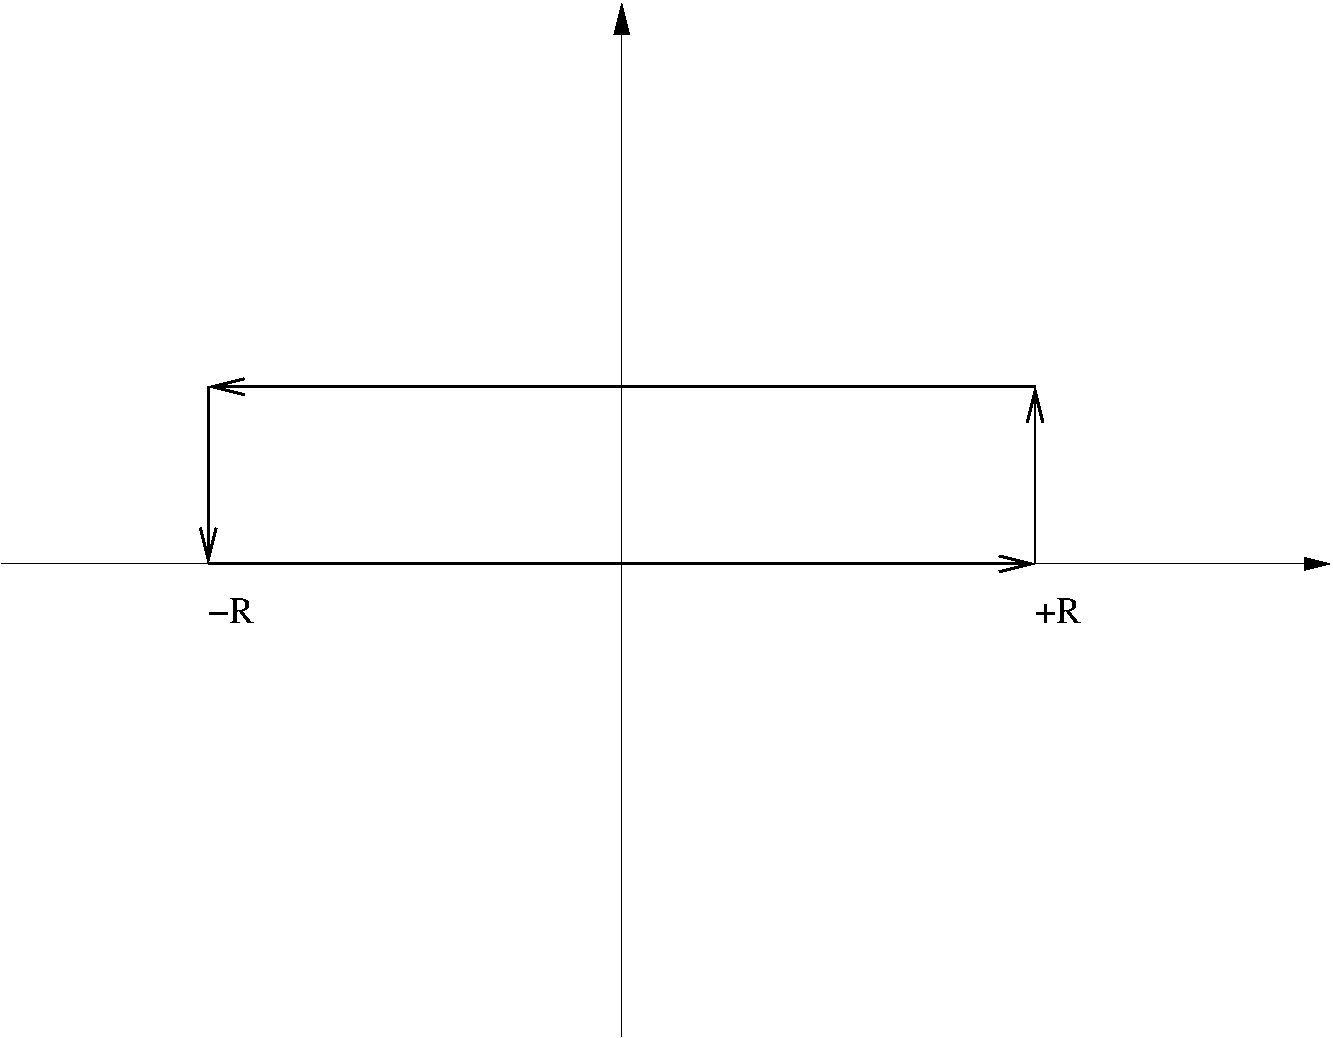
\includegraphics[scale=0.3]{images/contour_gauss.pdf}
\caption{Contour $\gamma_r$}\label{fig:contour3}
\end{figure}

La formule \ref{thm:stokes_complexe} montre qu'une application holomorphe et de dérivée continue dans un domaine (éventuellement avec des trous) a une intégrale nulle le long du bord. Nous allons maintenant montrer que cette propriété subsiste sous des hypothèses plus larges. 
\begin{fdefn}
Un lacet triangulaire de sommets $z_0,z_1,z_2$ est un lacet simple régulier de
classe $C^1$ par morceaux qui constitue le bord d'un triangle du plan complexe
de sommets $z_0,z_1,z_2$.
\end{fdefn}

Ce type de chemins joue un rôle particulier en théorie de l'intégration. La
propriété suivante est simple, mais fondamentale.

\begin{fprop}(Existence d'une primitive locale)
Soit $\Omega$ un domaine de $\mathbb{C}$ et $f \colon \Omega \to \mathbb{C}$ une
application continue. Si l'intégrale de $f$ le long de tout lacet triangulaire
de $\Omega$ est nulle, alors au voisinage de tout point $z_0 \in \Omega$, il
existe une application holomorphe $F$ de dérivée égale à $f$.
\end{fprop}

\begin{proof}
Soit $z_0 \in \Omega$ et soit $B_{z_0}$ une boule ouverte centrée en $z_0$ et
contenue dans $\Omega$. On pose, pour tout $z \in
B_{z_0}$:
\[
F(z) = \int_0^1 f(z_0 + t(z-z_0))(z-z_0) dt
\]
Soit maintenant $z \in B_{z_0}$ et soit $h \in \mathbb{C}$ tel que
$z+h \in B_{z_0}$. On a, en considérant le lacet triangulaire figure
\ref{fig:morera}:
\begin{align*}
F(z+h)-F(z) &= \int_0^1 f(z_0 + t(z-z_0))(z-z_0) dt \\
& - \int_0^1 f(z_0 +
(1-t)(z + h -z_0))(z + h-z_0) dt \\
&= \int_0^1 f(z+th)h dt 
\end{align*}
Par continuité de $f$, on en déduit:
\[
\lim_{h \to 0} \frac{F(z+h)-F(z)}{h} = f(z)
\]
ce qui prouve que $F$ est holomorphe, de dérivée $f$ en tout point de
$B_{z_0}$. 
\end{proof}
 \begin{figure}[ht]
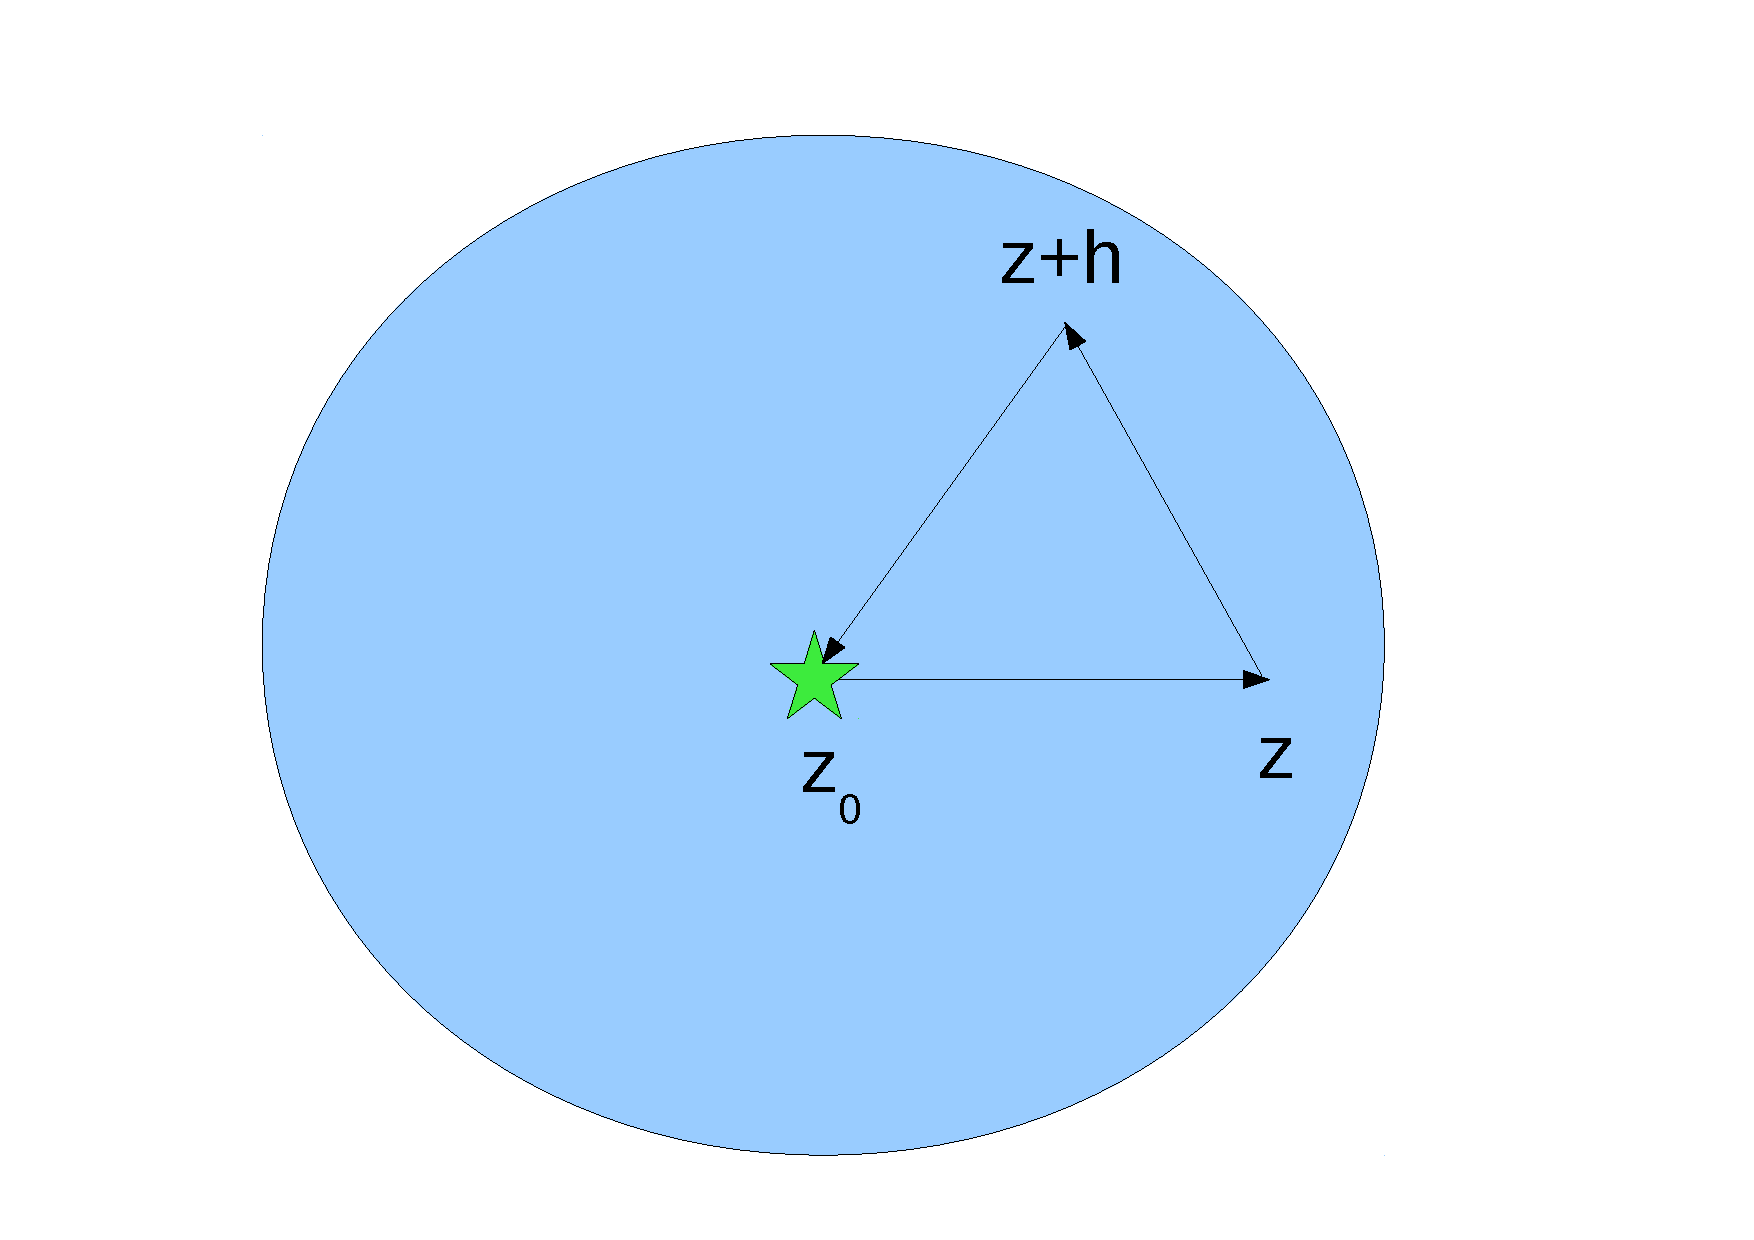
\includegraphics[scale=0.3]{images/morera.pdf}
\caption{Lacet triangulaire}\label{fig:morera}
\end{figure}
On notera que si $F$ est une primitive locale, il en est de même pour $F+K$ où
$K$ est un complexe quelconque.

\begin{fprop}(Primitive le long d'un chemin)
Soit $\Omega$ un domaine de $\mathbb{C}$ et soit $f$ vérifiant les hypothèses
de la proposition précédente. Soit $\gamma$ un chemin de $\Omega$. Il existe
alors une application continue $\theta \colon [0,1] \to \mathbb{C}$ telle 
que pour tout $t \in [0,1]$, il existe un voisinage $V_t$ de $\gamma(t)$
dans $\Omega$, une application $F$, holomorphe de classe $C^1$ sur $V_t$, de
dérivée égale à $f$ et vérifiant $\theta(u)=F(\gamma(u))$ au voisinage de $t$.
\end{fprop}

\begin{proof}
On va montrer par un procédé constructif la possibilité d'obtenir $\theta$. On
choisit tout d'abord $\theta_0$ de façon arbitraire. L'image de $\gamma$ est
un compact, on peut donc la recouvrir par un nombre fini de boules ouvertes
$B_i, i=1\dots N$ sur lesquelles on peut obtenir (proposition
précédente) une application $F_i$ holomorphe de classe $C^1$ et telle que
$F_i^\prime = f$. De plus, quitte à réordonner la numérotation des boules $B_i$,
on peut obtenir une subdivision $0=t_0 < t_2 < \dots < t_N = 1$ de $[0,1]$
telle que $\gamma([t_{i-1},t_i])\subset B_i, i =1\dots N$. 
 On peut choisir $F_1$ de telle sorte que
$F_1(\gamma(0))=\theta_0$ et on pose pour $u \in [t_0,t_1]$,
$\theta(u)=F_1(\gamma(u))$.
Supposons obtenue $\theta$ jusqu'à $t_i$. Sur le domaine $B_i \cap B_{i+1}$, la
différence entre $F_i,F_{i+1}$ est de dérivée nulle, donc cette différence est
constante. On peut choisir $F_{i+1}$ de telle sorte qu'elle soit nulle, ce qui
définit $\theta$ de proche en proche.
\end{proof}
Dans le cas où une application vérifie les hypothèses de la proposition
précédente, on peut définir de façon simple une notion d'intégrale le long du
chemin $\gamma$. Si $\theta$ est une primitive de $f$ le long de $\gamma$, on
posera:
\[
\int_{\gamma} f(z) dz = \theta(1)-\theta(0)
\] 
Cette définition coïncide avec celle donnée précédemment pour les chemins
de classe $C^1$ par morceaux, mais ne fait aucune autre hypothèse que la continuité sur
$\gamma$. En revanche, $f$ doit être continue et vérifier la condition
d'annulation de l'intégrale sur les lacets triangulaires.
L'intégrale est en général dépendante du chemin suivi. On a néanmoins une
invariance par homotopie, très importante pour la suite.
\begin{fdefn}
Soit $\Omega$ un domaine de $\mathbb{C}$ et  $\gamma_1, \gamma_2$ deux
chemins de $\Omega$ tels que $\gamma_1(0) = \gamma_2(0)$ et $\gamma_1(1) = \gamma_2(1)$. On dira que $\gamma_1$ et $\gamma_2$ sont homotopes à extrémités fixées si il existe une application continue:
\[
H \colon [0,1] \times [0,1] \to \Omega
\] 
telle que:
\begin{itemize}
\item $\forall t \in [0,1], \, H(0,t) = \gamma_1(t), \, H(1,t) = \gamma_2(t)$
\item $\forall s \in [0,1], \, H(s,0) = \gamma_1(0) = \gamma_2(0), \, H(s,1) = \gamma_1(1) = \gamma_2(1)$
\end{itemize}
\end{fdefn}
\begin{fthm}(Invariance par homotopie)
Soit $\Omega$ un domaine de $\mathbb{C}$ et soient $\gamma_1, \gamma_2$ deux
chemins de $\Omega$, homotopes à extrémités fixées. Soit $f \colon
\Omega \to \mathbb{C}$ continue et dont l'intégrale le long de tout lacet
triangulaire de $\Omega$ s'annule. Alors:
\[
\int_{\gamma_1} f(z) dz = \int_{\gamma_2} f(z) dz
 \]
\end{fthm}

\begin{proof}
 Soit $H$ l'homotopie entre $\gamma_1$ et $\gamma_2$. Pour tout
point $H(t,s)$, il existe une boule ouverte $B$ centrée sur ce point et contenue
dans $\Omega$ qui est ouvert. Par continuité de $H$, on en déduit l'existence
d'un pavé $]t_1,t_2[\times ]s_1,s_2[$ contenant $(t,s)$ et dont l'image est dans
$B$. La collection de ces pavés forme un recouvrement du compact
$[0,1]\times[0,1]$, il en existe donc une famille finie $\mathcal{S}$ qui
constitue aussi un recouvrement. Comme $\mathcal{S}$ est finie, on peut
construire une subdivision de $[0,1]\times[0,1]$ sous la forme de pavés
$\Delta_{ij}=[t_i, t_{i+1}]\times [s_j,s_{j+1}], \, i=0\dots N-1, j=0,\dots M-1$
avec $t_0=s_0=0$, $t_N=s_M=1$ tels que pour tout couple $(i,j)$,
$H(\Delta_{ij})$ est inclus dans un des membres de la famille $\mathcal{S}$. 
L'intégrale de $f$ étant nulle le long de tout lacet triangulaire, elle admet
une primitive dans chacune des boules de la famille $\mathcal{S}$ (reprendre la
démonstration précédente) et donc l'intégrale de $f$ le long du bord de
$\Delta_{ij}$ est nulle (différence de la primitive en deux points identiques).
De proche en proche, on en déduit que l'intégrale de $f$ le long des chemins $s \mapsto
H(t_i,s)$ est constante, soit finalement que l'intégrale de $f$ le long de
$\gamma_1$ est égale à celle le long de $\gamma_2$.
\end{proof}
L'invariance par homotopie montre en particulier que l'intégrale de $f$ le long
d'un lacet homotope à un lacet constant vaut $0$.

\begin{fdefn}
Soit $\Omega$ un domaine de $\mathbb{C}$. On appelle triangle de $\Omega$ de
sommets $z_1,z_2,z_3$ une partie $T \subset \Omega$ formée des combinaisons
barycentriques $\alpha_1 z_1 + \alpha_2 z_2 + \alpha_3 z_3$ où les
$\alpha_1,\alpha_2,\alpha_3$ appartiennent à $[0,1]$ et
$\alpha_1+\alpha_2+\alpha_3=1$.
\end{fdefn}

Le bord d'un triangle est un lacet triangulaire.

\begin{fthm}(Goursat)
Soit $\Omega$ un domaine de $\mathbb{C}$ et soit $f$ une application holomorphe
dans $\Omega$. Alors pour tout triangle $T$ de $\Omega$, l'intégrale de 
$f$ sur le bord de $T$ est nulle.
\end{fthm}

\begin{proof}
Le théorème de Goursat utilise un argument de division. Soit $T_0$ un 
triangle de $\Omega$ et soit $T_n$ une suite de fermés obtenus par
subdivision de $T_0$, ainsi que mentionné figure \ref{fig:sub_triang}. En posant
$d$ le diamètre de $T_0$ et $p$ son périmètre, on vérifie facilement que le
diamètre des triangles de $T_n$ est $d 2^{-n}$ et que le périmètre est $p
2^{-n}$. Soit $\epsilon > 0$. Il existe, pour tout $z$ intérieur à $T_0$, une
boule ouverte $B_z$ telle que:
\[
\forall u \in B_z, |f(u)-f(z)-f^\prime(z)(u-z)| < \epsilon |u-z|
\]
$T_0$ étant compact, un nombre fini de boules $B_z$ le recouvre. Il existe donc
une subdivision $T_n$ telle que chaque triangle la constituant soit dans l'une
de ces boules. L'application  $u \mapsto f(z)+f^\prime(z)(u-z)$ est un polynôme,
donc holomorphe et de dérivée continue: son intégrale sera nulle sur le
bord chaque triangle de $T_n$. Soit $T$ un triangle de $T_n$ contenu dans la boule $B_z$. 
On a:
\begin{align*}
& \left|
\int_{\partial T} f(u) du
\right| \leq  \\ &\int_{\partial T}  |f(u)-f(z)-f^\prime(z)(u-z)| du + \left |
\int_{\partial T} f(z)+f^\prime(z)(u-z) \right| du \leq \\
& \int_{\partial T}  |f(u)-f(z)-f^\prime(z)(u-z)| du \leq \\
& \epsilon d p 4^{-n}
\end{align*}
$T_n$ étant formé d'exactement $4^n$ triangles, on a par sommation:
\[
\left| \int_{\partial T_0} f(u) du \right| < \epsilon d p
\]
Comme $\epsilon$ est arbitraire, on en déduit que l'intégrale est nulle.
\end{proof}
 \begin{figure}[ht]
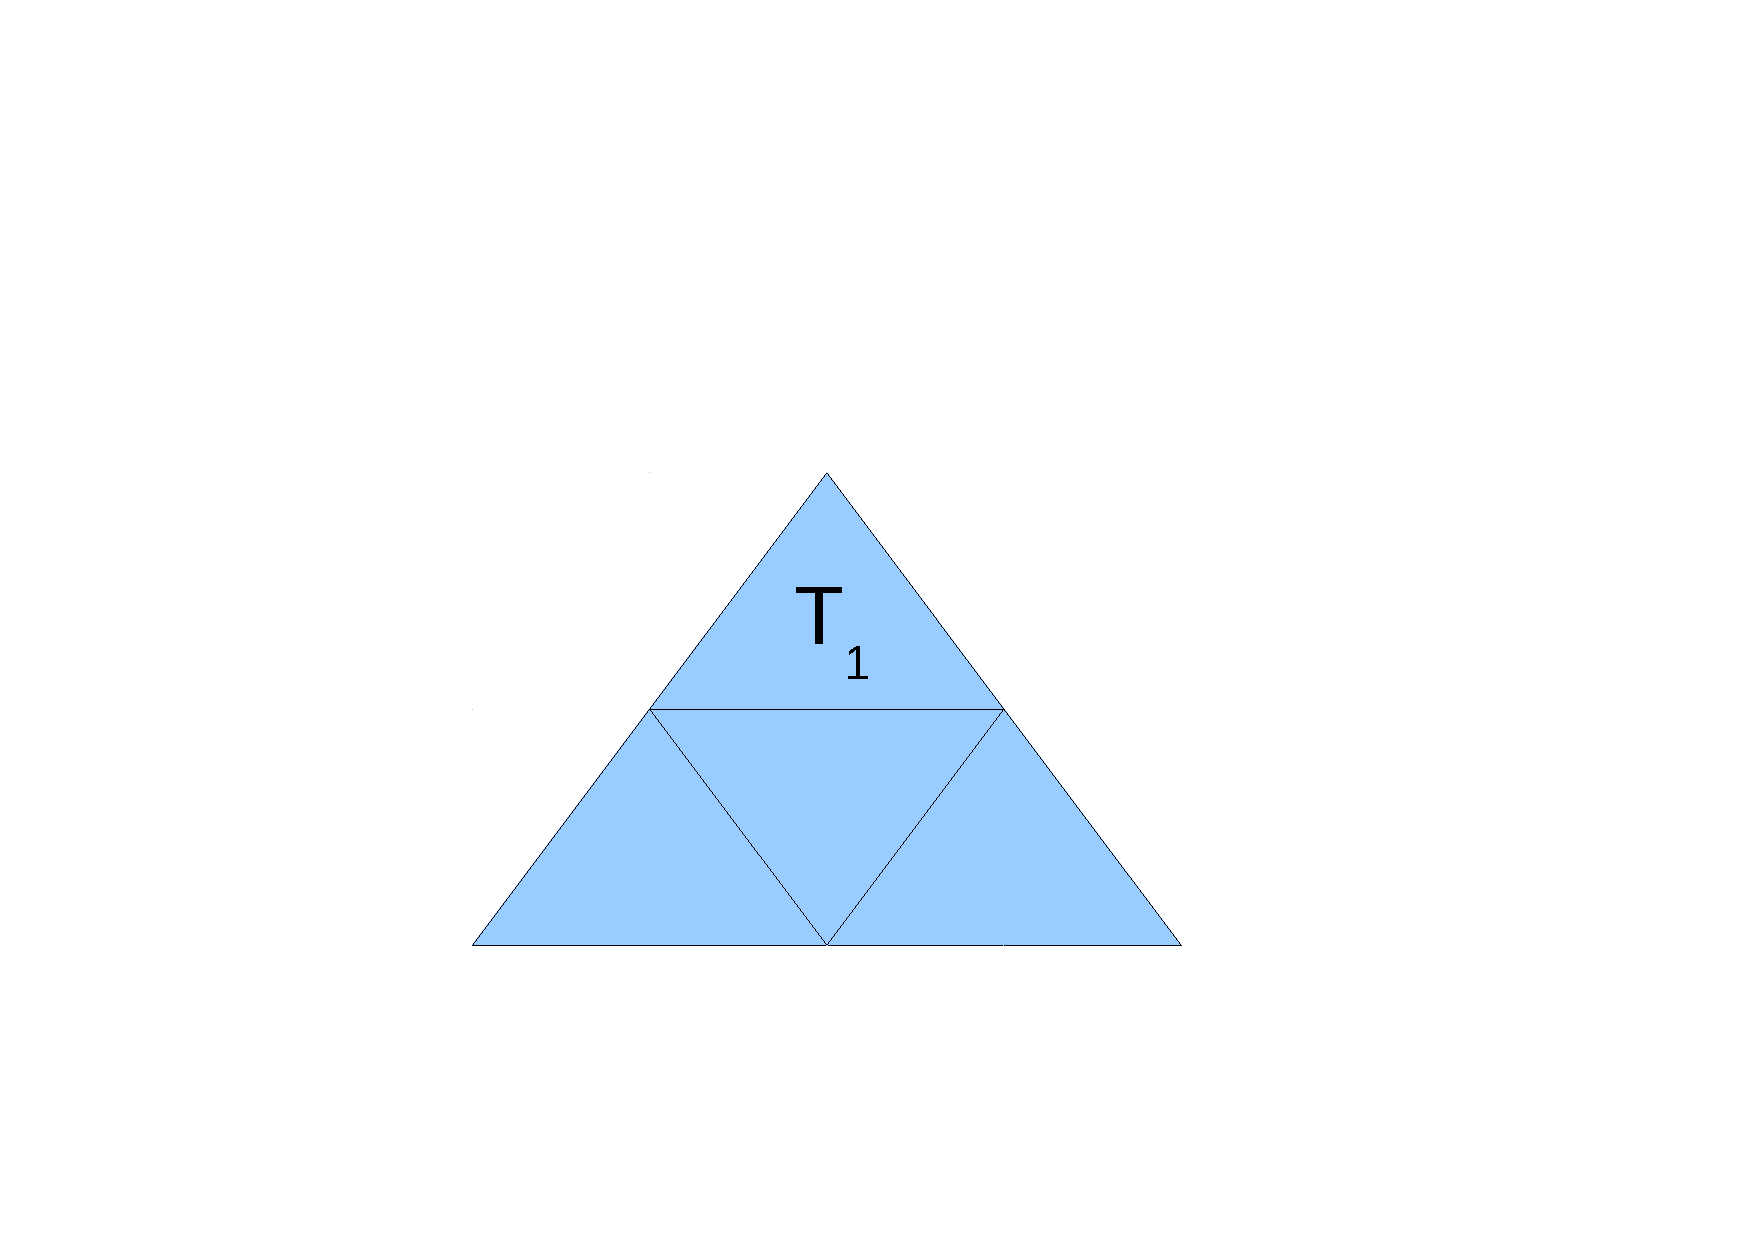
\includegraphics[scale=0.3]{images/subdivision_triangle.pdf}
\caption{Passage de $T_0$ à $T_1$ par subdivision}\label{fig:sub_triang}
\end{figure}
Le théorème de Goursat est encore vrai si l'on suppose seulement l'holomorphie
sur $\Omega$ privé d'une droite et la continuité sur $\Omega$: si la droite en
question coupe un chemin triangulaire on se ramènera par continuité et
subdivision au cas précédent. Dans un domaine $1$-connexe, on a le très important théorème suivant:

\begin{fthm}
Soit $\Omega$ un domaine simplement connexe. Soit $f$ une application holomorphe
dans $\mathbb{C}$. Alors $f$ admet une primitive le long de tout chemin de
$\Omega$ et l'intégrale de $f$ sur tout lacet de $\Omega$ est nulle.
\end{fthm}

\begin{proof}
Le théorème de Goursat montre l'existence d'une primitive pour $f$ le long de
tout chemin de $\Omega$. Le domaine étant simplement connexe, tout lacet est
homotope à un lacet constant: l'intégrale de $f$ le long de tout lacet est
nulle.
 \end{proof}
 Le théorème précédent donne aussi une primitive globale $F$ pour $f$: il
 suffit à cet effet de se donner la valeur de $F$ en un point $z_0 \in \Omega$
 et de poser:
 \[
 F(z) = F(z_0) + \int_{\gamma} f(z)dz
 \]
 avec $\gamma$ chemin d'origine $z_0$ et d'extrémité $z$. L'intégrale de $f$
 est nulle sur tout lacet, la valeur de $F$ en $z$ ne dépend donc pas du chemin
 choisi.
\section{Formules de Cauchy}

\begin{fdefn}(Calcul de l'indice par intégrale curviligne)
Soit $\gamma$ un lacet et  soit $z_0 \in \mathbb{C}$ n'appartenant pas à l'image
de $\gamma$. L'indice de $\gamma$ par rapport à $z_0$ est:
\[
I(\gamma;z_0) = \frac{1}{i 2 \pi}\int_{\gamma} \frac{1}{z-z_0}dz
\]
\end{fdefn}
L'indice d'un lacet compte le nombre de tours effectués par $\gamma$ autour de $z_0$, positivement dans le sens trigonométrique et négativement en sens opposé. On peut établir cette propriété en raisonnant en deux temps. Sans perte de généralité, on supposera que $z_0 = 0$. On note tout d'abord que si $\gamma$ ne passe pas par 0, il existe une boule fermée $B(0,r)$ ne rencontrant pas $\gamma$. L'application:
\[
H \colon (s,t) \in [0,1] \times [0,1] \mapsto s \frac{r \gamma(t)}{|\gamma(t)|} + (1-s) \gamma(t)
\] 
établit une homotopie dans $C^*$ entre $\gamma$ et un lacet $\tilde{\gamma} = H(1,\bullet)$ dont l'image appartient au cercle $\mathcal{C}_r$ de centre 0 et de rayon $r$. En vertu du théorème d'invariance homotopique, l'indice de $\tilde{\gamma}$ est le même que celui de $\gamma$. Au voisinage de $\mathcal{C}_r$, l'application:
\[
\ln \left(z = |z|\exp(i \theta) \right) = \ln |z| + i (\theta+ 2 k \pi), \theta \in [0, 2 \pi [ , k \in \Z
\]
définit une primitive locale de l'application $z^{-1}$ et la conclusion s'ensuit (faire un dessin et propager les écarts angulaires \dots). 
\begin{fthm}(Première formule de Cauchy)
Soit $\Omega$ un domaine simplement connexe de $\mathbb{C}$ et $f$ holomorphe
dans $\Omega$. Soit $\gamma$ un lacet de $\Omega$ et $z_0$ n'appartenant pas à
l'image de $\gamma$. On a:
\[
\int_{\gamma} \frac{f(z)}{z-z_0} dz = i 2 \pi I(\gamma; z_0)f(z_0)
\]
\end{fthm}
\begin{proof}
Soit l'application:
\[
F \colon z \mapsto \left \{
\begin{array}{cc} 
\frac{f(z)-f(z_0)}{z-z_0} & z \neq z_0 \\
f^\prime(z_0) & z = z_0
\end{array}
\right.
\]
$F$ est holomorphe dans $\Omega - \{z_0\}$, continue sur $\Omega$: le théorème
de Goursat (forme étendue) montre que l'intégrale de $F$ le long de $\gamma$ est
nulle, la conclusion est obtenue avec la proposition établie sur le calcul de
l'indice par intégrale curviligne.
\end{proof}
La formule de Cauchy peut également s'énoncer dans le cas d'un domaine dont le
bord est un lacet simple régulier de classe $C^1$ par morceaux:

\begin{fprop}
Soit $\Omega$ un domaine de bord $\partial \Omega$ un lacet simple régulier de classe $C^1$ et soit $f$ une application holomorphe dans $\Omega$,
continue sur $\partial \Omega$. Pour tout point $z_0 \in \Omega$ on a:
\[
\int_{\gamma} \frac{f(z)}{z-z_0} dz = i 2 \pi f(z_0)
\]
\end{fprop}
 
La preuve est similaire au cas précédent, mais utilise le théorème basé sur la
formule de Stokes.
 La formule de Cauchy se généralise immédiatement au cas d'un domaine
 $n$-connexe dont le bord est constitué d'une union finie de lacets simples rectifiables, en se ramenant à un ouvert simplement connexe. On prendra
garde néanmoins au sens de parcours du lacet.

 \begin{fthm}(Seconde formule
de Cauchy) Sous les même hypothèses que la première formule de Cauchy, on a~:
\[
I(\gamma; z_0) f^\prime(z_0) = \frac{1}{i 2 \pi} \int_{\gamma}
\frac{f(z)}{(z-z_0)^2} dz
\]
\end{fthm}

\begin{proof}
On supposera l'indice du lacet $\gamma$ égal à 1 pour simplifier les écritures.
Formons le rapport~:
\[
\frac{f(z_0+h)-f(z_0)}{h} = \frac{1}{i 2
\pi}\int_{\gamma}\frac{f(z)}{(z-z_0)(z-z_0-h)} dz
\]
avec $h$ tel que $z_0+h \in \Omega$. En passant à la limite $|h|\to +\infty$, on
obtient le résultat.
\end{proof}

Par récurrence, on obtient les dérivées d'ordre supérieur~:
\[
I(\gamma; z_0) f^{(n)}(z_0) = \frac{n!}{i 2 \pi} \int_{\gamma}
\frac{f(z)}{(z-z_0)^{n+1}} dz
\]
Enfin, il est possible d'obtenir une formulation utilisant la formule de Stokes
(la démonstration n'est pas détaillée).

\begin{fthm}
Soit $f$ holomorphe dans un domaine $\Omega$ dont le bord est un lacet simple régulier de classe $C^1$ par morceaux. Si $f$ est continue sur
$\partial \Omega$, elle est indéfiniment dérivable en tout $z_0 \in \Omega$ et~:
\[
f^{(n)}(z_0) =  \frac{n!}{i 2 \pi} \int_{\gamma} \frac{f(z)}{(z-z_0)^{n+1}} dz
\]
\end{fthm}

Les formules intégrales de Cauchy montrent qu'une application holomorphe dans un
domaine y est indéfiniment dérivable. On peut aussi utiliser ces formules pour
évaluer des intégrales:
\begin{exercice}
Soit $f$ l'application définie par:
\[
f \colon z \mapsto \frac{\exp(iaz)}{1+z^2}
\]
avec $a>0$ réel. 
\begin{itemize}
  \item En utilisant la première formule de Cauchy, évaluer l'intégrale de $f$
  le long du contour donné figure \ref{fig:contour_ex1} et sous l'hypothèse
  $R>1$.
  \item Par passage à la limite $R \to +\infty$, en déduire la transformée de
  Fourier de l'application $x \mapsto (1+x^2)^{-1}$.
\end{itemize}
\end{exercice}
\begin{figure}[ht]
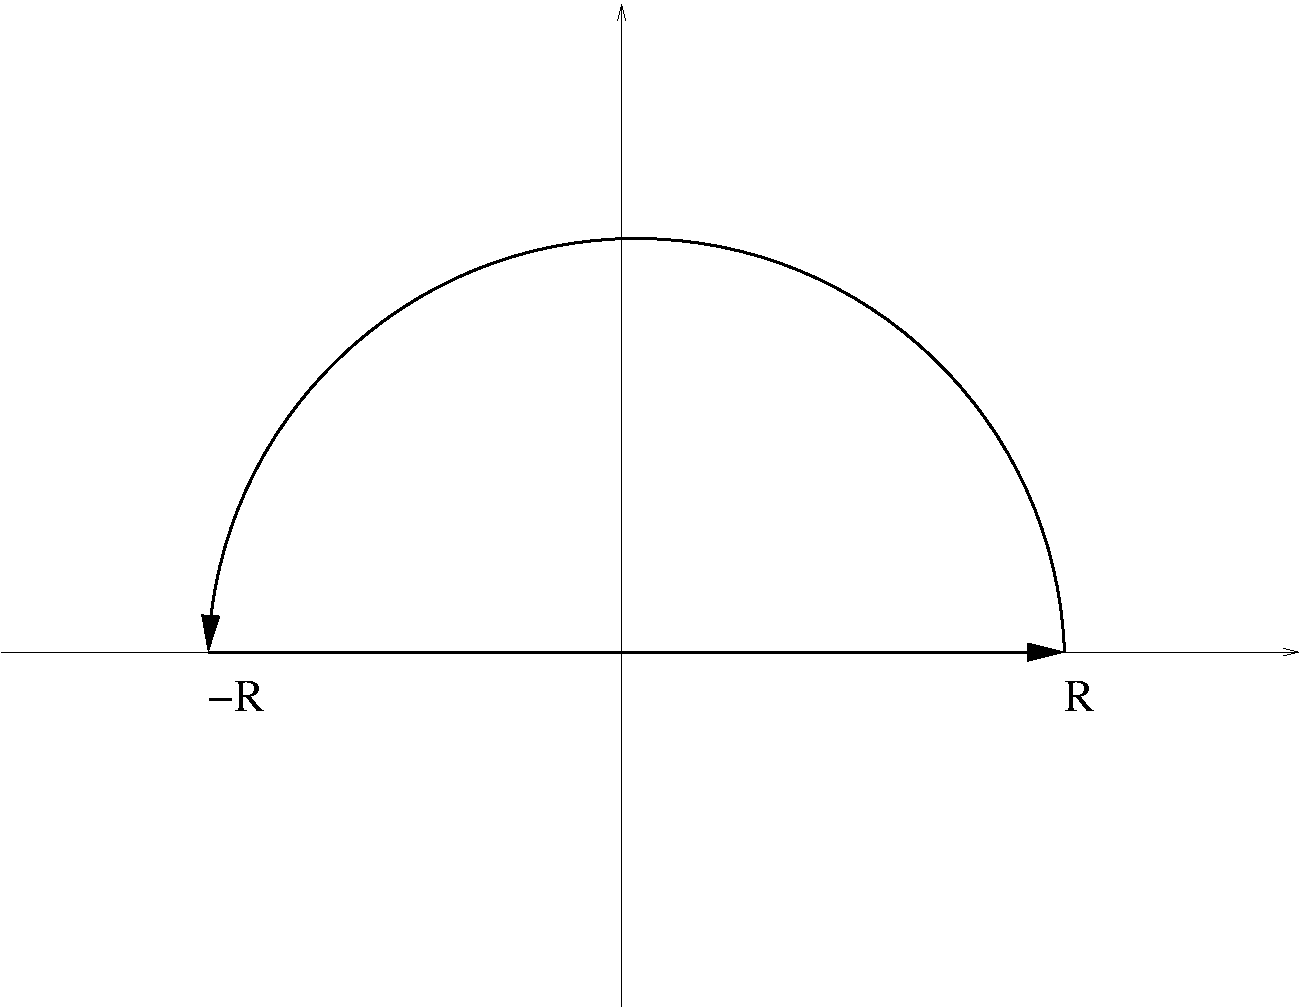
\includegraphics[scale=0.3]{images/contour_ex1.pdf}
\caption{Contour d'intégration}\label{fig:contour_ex1}
\end{figure}
\subsection{Calcul numérique}
Le théorème de Stokes complexe peut être utilisé pour calculer 
numériquement la surface du domaine $\Omega$ entouré par un lacet polygonal $\gamma$. Si 
l'on se donne ce dernier par une liste de sommets $(z_i), \, i=0 \dots N-1$ on peut paramétrer le chemin liant le sommet $i$ au sommet $i+1$ comme:
\[
\gamma_i \colon t \in [0,1] \mapsto z_i + t\left(z_{i+1}-z_i\right)
\]
Sur cette partie du lacet, on formera l'intégrale:
\[
\int_{\gamma_i}\overline{z}dz = \int_{[0,1]}\left(\overline{ z_i}+t \overline{\left(z_{i+1}-z_i\right)}\right)\left(z_{i+1}-z_i\right) dt=
\frac{\overline{z_{i+1}}+\overline{z_i}}{2}\left(z_{i+1}-z_i\right)
\]
et par la formule de Stokes complexe:
\[
\sum_{i=0}^{N-1}\frac{\overline{z_{i+1}}+\overline{z_i}}{2}\left(z_{i+1}-z_i\right) = - \int_{\Omega} dz d\overline{z}
\]
Comme:
\[
\int_{\Omega} dz d\overline{z} = - 2 i \int_{\Omega} dx dy
\]
on en déduit que la surface de $\Omega$ est égale à:
\[
- i \sum_{i=0}^{N-1}\frac{\overline{z_{i+1}}+\overline{z_i}}{4}\left(z_{i+1}-z_i\right)
\]
En développant, on obtient:
\[
- \frac{i}{4} \sum_{i=0}^{N-1} \left(\left|z_{i+1}\right|^2 - \left|z_i \right|^2 + 2 i \Im \left(z_{i+1}\overline{z_i} \right)
\right)
\]
On peut vérifier sans difficultés que les termes en module carré se simplifient deux à deux dans la somme (se rappeler que $z_N = z_0$). La surface est donc en final:
\[
\frac{1}{2} \sum_{i=0}^{N-1} \Im \left(z_{i+1}\overline{z_i} \right)
\]
Enfin, on remarque que pour tout couple $(z_1=x_1+iy_1, z_2=x_2+iy_2)$ le produit $z_2 \overline{z_1}$ a pour partie réelle le produit scalaire des vecteurs $(x_1,y_1)$ et $(x_2,y_2)$ et pour partie réelle leur déterminant. Ceci donne une interprétation géométrique à la formule de sommation précédente, le déterminant de deux vecteurs orientés en sens direct s'identifiant à la surface du parallélogramme qu'ils définissent. Le code python ci-dessous implémente le calcul de surface tel qu'il vient d'être énoncé. 
\begin{verbatim}
# -*- coding: utf8 -*-
import math


# classe point
class Point:
    def __init__(self,x=0.0,y=0.0):
        self.x=x
        self.y=y
# classe lacet
class Lacet:
    # constructeur. La liste de points est initialement vide
    def __init__(self):
        self.point_list=[]
    # ajoute un point à la liste définissant le lacet
    # p : point
    def add(self,p):
        self.point_list.append(p)
    # calcule la surface entourée par le lacet
    # return: réel
    def surface(self):
        surf = 0.0
        n = len(self.point_list)-1
        for i in range(n):
            surf = surf-self.point_list[i+1].x*self.point_list[i].y\
             + self.point_list[i+1].y * self.point_list[i].x
        	surf = surf - self.point_list[0].x*self.point_list[n].y\
        	 + self.point_list[0].y*self.point_list[n].x
        return 0.5 * surf
# test
gamma=Lacet()
gamma.add(Point(1.0,0.0))
gamma.add(Point(0.0,1.0))
gamma.add(Point(-1.0,0.0))
gamma.add(Point(0.0,-1.0))

print(gamma.surface())

gamma=Lacet()
gamma.add(Point(1.0,1.0))
gamma.add(Point(-1.0,1.0))
gamma.add(Point(-1.0,-1.0))
gamma.add(Point(1.0,-1.0))

print(gamma.surface())
\end{verbatim}
A titre d'exercice, améliorer le code pour inclure des lacets définis par des segments de droites et des arcs de cercle. 
\newpage
\leftline{\textbf{Un peu d'histoire \dots}}
\vskip 12pt
\begin{tabular}{ll}
\multicolumn{2}{l}{\textbf{Augustin Louis Cauchy}} \\[10pt]
\begin{minipage}{0.2\linewidth}
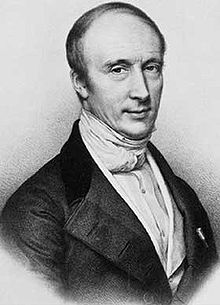
\includegraphics[scale=0.4]{images/Cauchy.jpg}
\end{minipage}
&
\begin{minipage}{0.65\linewidth}
Né le  né à Paris le 21 août 1789 et mort à Sceaux (Hauts-de-Seine) le 23 mai 1857. C'est un des mathématiciens les plus productifs connus (800 publications à son actif). Ses travaux ont concerné la plupart des domaines des mathématiques de son époque: analyse, algèbre, géométrie, probabilités. On lui doit le critère qui porte son nom pour les suites et est à l'origine de la théorie de l'intégration complexe. 
\end{minipage}\\
\multicolumn{2}{l}{\textbf{Edouard Goursat}} \\[10pt]
\begin{minipage}{0.2\linewidth}
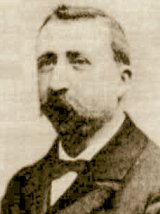
\includegraphics[scale=0.4]{images/Goursat.jpg}
\end{minipage}
&
\begin{minipage}{0.65\linewidth}
 Né le 21 mai 1858 à Lanzac (Lot) et mort le 25 novembre 1936 à Paris. Il travailla sur les fonctions de la variable complexe et prouva le lemme qui porte son nom. Son cours d'analyse a été longtemps une référence.
\end{minipage}
\end{tabular}
\chapter{Théorème des résidus}
\section{Développement en série de Laurent}
Cette section est à connaître en totalité.
\subsection{Série de Taylor d'une application holomorphe}
Soit dans le plan complexe le disque ouvert $D$ de centre $z_0$ et de rayon
$r>0$. Le bord $\partial D$ est le cercle $\mathcal{C}$ de centre $z_0$ et de
rayon $r$ (voir \ref{Fi:Taylor}. Soit $f$ une application $\overline{D} \to
\mathbb{C}$ holomorphe dans $D$ et continue sur $\mathcal{C}$.
\begin{figure}
\scalebox{.68}{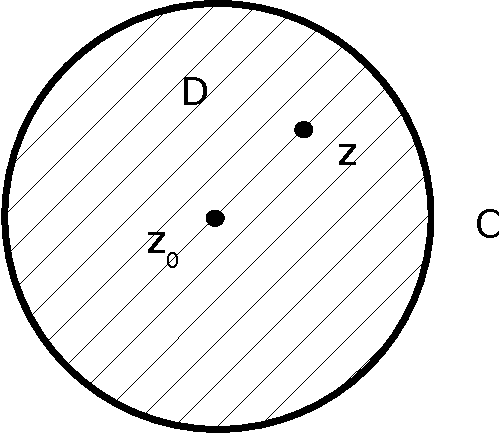
\includegraphics{images/taylor.pdf}}
\caption{Domaine D}\label{Fi:Taylor}
\end{figure}
En un point de $z \in D$, la formule de Cauchy permet d'écrire~:
\[
f(z) = \frac{1}{i2\pi}\int_{\mathcal{C}} \frac{f(u)}{u-z} du
\]
Soit, en faisant intervenir le point $z_0$~:
\[
f(z) = \frac{1}{i2\pi}\int_{\mathcal{C}} \frac{f(u)}{(u-z_0)-(z-z_0)} du =
\frac{1}{i2\pi}\int_{\mathcal{C}}
\frac{1}{u-z_0}\frac{f(u)}{1-\frac{z-z_0}{u-z_0}} du
\]
Pour $N \in \mathbb{N}$ fixé, on a~:
\[
\frac{1}{1-\frac{z-z_0}{u-z_0}} = \sum_{n=0}^N \left ( \frac{z-z_0}{u-z_0}
\right )^n + \left ( \frac{z-z_0}{u-z_0}
\right )^{N+1} \frac{1}{(u-z_0)-(z-z_0)}
\]
L'application $f$ étant par hypothèse continue sur le compact $\mathcal{C}$,
il existe un réel $M$ tel que $|f(z)|\leq M, z \in \mathcal{C}$. L'intégrale~:
\[
\int_{\mathcal{C}} \left ( \frac{z-z_0}{u-z_0}
\right )^{N+1} \frac{f(u)}{(u-z_0)-(z-z_0)} du 
\]
est bornée en module par~:
\[
\left ( \frac{|z-z_0|}{r}
\right )^{N+1} \frac{Mr}{r-|z-z_0|}
\]
Comme~:
\[
\left ( \frac{|z-z_0|}{r}
\right ) < 1
\]
On en déduit la convergence de la série~:
\[
f(z) = \frac{1}{i2\pi}\int_{\mathcal{C}}
\frac{f(u)}{u-z_0}\sum_{n \in \mathbb{N}} \left ( \frac{z-z_0}{u-z_0} \right )^n
du
\]
Par application de la formule de Cauchy~:
\[
\frac{1}{i2\pi} \int_{\mathcal{C}}
\frac{f(u)}{(u-z_0)^{n+1}} = \frac{f^{(n)}(z_0)}{n!}
\]
D'où finalement l'expression du développement en série de Taylor de $f$ en tout
point $z \in D$~:
\[
f(z)= \sum_{n\in \mathbb{N}} \frac{f^{(n)}(z_0)}{n!} (z-z_0)^n
\]
Il est clair que le développement en série de Taylor de $f$ dans $D$ est
unique.

\subsection{Développement au voisinage d'un point singulier isolé}
En utilisant les mêmes notations que dans la section précédente, on supposera
maintenant que $f$ est holomorphe dans l'ouvert $D- \{ z_0 \}$.
Soit $r_1$ vérifiant~:$r > r_1 > 0$. L'application $f$ est holomorphe dans
la couronne ouverte $\mathcal{C}$ de centre $z_0$, de rayon extérieur $r$ et de
rayon intérieur $r_1$. Le bord de cette couronne est la réunion des deux
cercles $\mathcal{C}_1, \mathcal{C}_2$ de centre $z_0$ et de rayons respectifs
$r$ et $r_1$. Le cercle $\mathcal{C}_1$ sera orienté positivement en sens
trigonométrique, le cercle $\mathcal{C}_2$ sera orienté en sens inverse
trigonométrique (le bord reçoit ainsi son orientation canonique). Par
application de la formule de Cauchy et en tenant compte de l'orientation de
$\mathcal{C}_2$, on obtient pour tout $z \in \mathcal{C}$~:
\[
f(z) = \frac{1}{i2 \pi} \int_{\mathcal{C}_1} \frac{f(u)}{u-z}du - \frac{1}{i2
\pi} \int_{\mathcal{C}_2} \frac{f(u)}{u-z}du
\]
La première intégrale de la partie droite se développe de la même façon que
précédemment et l'on obtient~:
\[
\frac{1}{i2 \pi} \int_{\mathcal{C}_1} \frac{f(u)}{u-z}du = \sum_{n \geq 0} a_n
(z-z_0)^n
\]
avec~:
\[
a_n = \frac{1}{i2\pi} \int_{\mathcal{C}_1} \frac{f(u)}{(u-z_0)^{n+1}}du
\]
\begin{rem}
Bien prendre garde à ne pas écrire $a_n=\frac{f^{(n)}(z_0)}{n!}$ car $f$ n'est
pas supposée holomorphe au voisinage de $z_0$.
\end{rem}
Pour la seconde intégrale, on utilisera l'expression suivante~:
\[
\frac{1}{z-u} = \frac{1}{(z-z_0)-(u-z_0)} = \frac{1}{z-z_0}\frac{1}{1-
\frac{u-z_0}{z-z_0}}
\]
En procédant de la même façon que pour la série de Taylor, et en remarquant que
pour $u \in \mathcal{C}_2$~:
\[
\left | \frac{u-z_0}{z-z_0} \right | < 1
\]
on obtient l'expression suivante~:
\[
- \frac{1}{i 2 \pi} 
\int_{\mathcal{C}_2} \frac{f(u)}{u-z}du = \sum_{n \geq 1} b_n
\frac{1}{(z-z_0)^n}
\]
avec~:
\[
b_n = \frac{1}{i2\pi} \int_{\mathcal{C}_2} (u-z_0)^{n-1}f(u) du
\]
Le développement correspondant~:
\[
f(z) = \sum_{n \geq 0} a_n
(z-z_0)^n + \sum_{n \geq 1} b_n (z-z_0)^{-n}
\]
s'appelle développement en série de Laurent de $f$ dans la couronne
$\mathcal{C}$.
Le développement en série de Laurent est unique.
On notera, avec les hypothèses faites sur $f$, que les coefficients
$(a_n),(b_n)$ ne dépendent pas du rayon intérieur $r_1$. On distinguera trois
cas~:
\begin{itemize}
  \item Les coefficients $(b_n)$ sont tous nuls. Dans ce cas, on peut prolonger
  $f$ analytiquement en $z_0$ en posant $f(z_0)=a_0$. 
  \item Les coefficients $(b_n)$ sont nuls à partir d'un certain rang. Soit $p$
  le plus petit entier tel que $b_p \neq 0$ et $\forall n > p, b_n = 0$.
  L'application $z \mapsto (z-z_0)^p f(z)$ admet un prolongement analytique en
  $z_0$. On dira dans ce cas que $z_0$ est un pôle d'ordre $p$.
  \item Dans les autres cas, on dira que $z_0$ est un point singulier essentiel.
\end{itemize}
\begin{rem}
L'unicité du développement en série de Laurent permet souvent de calculer les
coefficients $(a_n)$ ou $(b_n)$ à partir de développement connus. Par exemple,
dans une couronne centrée en $0$, on aura~:
\[
exp(z^{-1}) = 1 + \sum_{n \geq 1} \frac{1}{n!} z^{-n}
\]
d'où l'on déduit $a_0=1, a_n=0 , n > 0$ et $b_n=\frac{1}{n!}, n \geq 1$ dans ce
cas.
\end{rem}
\begin{rem}
Au voisinage d'un pôle d'ordre $p$, l'application $g \colon z \mapsto (z-z_0)^p
f(z)$ admet un prolongement analytique. on peut donc calculer son développement en
série de Taylor~:
\[
g(z) = \sum_{n \geq 0} c_n (z-z_0)^n
\]
avec~:
\[
c_n = \lim_{z \to z_0} \frac{1}{n!} g^{(n)}(z)
\]
Ceci permet d'évaluer facilement les termes $(b_n)$ du développement de $f$~:
\[
b_n = c_{p-n}
\]
\begin{defn}
Une application $f$ est dite méromorphe dans un ouvert $\Omega$ si elle ne
possède dans $\Omega$ pour seuls points singuliers des pôles.
\end{defn}
\end{rem}
\section{Théorème des résidus}
Les résultats de la section précédente permettent de développer une application
$f$ au voisinage d'un point singulier isolé $z_0$. On notera le lien existant
entre $b_1$ et l'intégrale de l'application sur le cercle intérieur d'une couronne
entourant le point singulier. Le coefficient $b_1$, en raison de son importance,
a reçu un nom particulier~: c'est le résidu de $f$ en $z_0$, noté $Res(f;z_0)$.

\begin{fthm}
Soit $\Omega$ un ouvert $1$-connexe et soit 
$\gamma$ un lacet de $\Omega$ . Soit $f$ une application holomorphe dans 
$\Omega-\{z_1, \dots z_n\}$ où les $z_i,i=1\dots n$ sont distincts deux à deux.
On~:
\[
\int_{\gamma} f(z) dz = i 2 \pi \sum_{j=1}^n Res(f;z_i)
\]
\end{fthm}

\begin{proof}
Il existe pour chaque $z_j$ une
couronne ouverte $\mathcal{C}_j$ de centre $z_j$ ne contenant aucun autre point
singulier. Le développement en série de Laurent sur chacune de ces couronnes
montre que~:
\[
Res_{z_j}f = \frac{1}{i 2 \pi} \int_{c_j} f(z) dz
\]
avec $c_j$ cercle intérieur de $\mathcal{C}_j$, orienté en sens
trigonométrique. L'application $f$ étant holomorphe dans $\Omega - \cup_{j=1}^n
D_j$ avec $D_j$ disque ouvert de centre $z_j$ et de bord $c_j$, on a~:
\[
\int_{\gamma} f(z) dz - \sum_{j=1}^n \int_{c_j} f(z)dz =0
\]
et le résultat s'en déduit.
\end{proof}
\begin{rem}
Le calcul pratique des résidus d'une application $f$ peut s'obtenir par
développement en série de Laurent. Dans le cas d'un pôle simple en $z_0$, on
retiendra que si $f(z)=p(z)/q(z)$, alors~:
\[
Res_{z_0}f = \frac{p(z_0)}{q^\prime(z_0)}
\]
Si on a affaire a un pôle d'ordre $p$, on utilisera la formule~:
\[
Res_{z_0}f = \lim_{z \to z_0} \frac{1}{(p-1)!}
\frac{d^{p-1}}{dz^{p-1}}[(z-z_0)f(z)]
\]
\end{rem}
Il existe comme toujours une forme utilisant la formule de Stokes:

\begin{fthm}
Soit $\Omega$ un domaine de bord un lacet simple régulier de classe $C^1$
par morceaux. Soit $f$ une application
holomorphe dans $\Omega-\{z_1, \dots z_n\}$ où les $z_i,i=1\dots n$ sont
distincts deux à deux, et continue sur $\partial \Omega$ On a~:
\[
\int_{\partial \Omega} f(z) dz = i 2 \pi \sum_{j=1}^n Res(f;z_i)
\]
\end{fthm}

Le théorème des résidus est la base du calcul des intégrales de chemin et permet
également d'évaluer de très nombreuses intégrales généralisées.
\begin{exercice}
Calculer les intégrales généralisées suivantes~:
\[
\begin{array}{l}
I_1 = \int_0^{+\infty} \frac{x^2 \cos(ax)}{1+x^4} dx , \quad a \in
\mathbb{R}\\
I_2 = \int_0^{+\infty} \frac{ \sin x}{x}dx
\end{array}
\]
\end{exercice}
\section{Calcul numérique}
Les développements en série de Laurent permettent souvent d'approcher numériquement une fonction inconnue ou très difficile à calculer par une fraction rationnelle complexe. Le site:
\url{http://dlmf.nist.gov/} recense de très nombreuses fonctions, avec des méthodes permettant de les calculer. On y trouvera des expressions sous formes de fractions continues, dont la troncature à un ordre fini donne une fraction rationnelle. Dans certains cas, une approximation rationnelle est beaucoup plus efficace qu'un développement en série de Taylor. 

On supposera dans la suite que la fonction $f$ que l'on souhaite approcher est connue de façon expérimentale, sous la forme d'un échantillon de couples de complexes $(z_i,w_i), i=0 \dots N-1$ avec $w_i = f\left(z_i\right)$. On recherchera une fraction rationnelle:
\[
\widetilde{f} \colon z \mapsto \frac{\sum_{k=0}^P a_k z^k}{\sum_{j=0}^Q b_j z^j}
\]
qui minimise l'erreur de calcul:
\[
\sum_{i=0}^{N-1} \left|w_i - \widetilde{f}(z_i)\right|^2
\] 
Sous cette forme, il est assez difficile de trouver le jeu de paramètres optimaux $(a_k),(b_j)$. Le problème sera donc reformulé comme la recherche des coefficients minimisant:
\[
\sum_{i=0}^{N-1} \left|w_i \sum_{j=0}^Q b_j z_i^j - 
\sum_{k=0}^P a_k z_i^k \right|^2
\] 
Ce problème est mal posé sous cette forme: rien ne change en effet si l'on multiplie les coefficients  $(a_k),(b_j)$ par un même nombre complexe. On lèvera cette indétermination en fixant un des coefficients à 1, typiquement $a_P$ ou $b_Q$ (on choisit ici de poser $a_P=1$). En se rappelant que la norme carrée d'un vecteur complexe s'écrit comme la somme des modules carrés de ses composantes, le critère précédent admet une formulation algébrique simple: il s'agit de trouver le vecteur complexe $v=(a_0, \dots,a_{P-1},b_0, \dots, b_Q)$ rendant minimum la norme carrée du vecteur:
\[
M v - 
\left(
\begin{array}{c}
z_0^P \\
z_1^P \\ 
\vdots \\ 
z_{N-1}^P
\end{array}
\right)
\]
avec $M$ la matrice:
\[
\left(
\begin{array}{cccccccc}
-1 & -z_0 & \dots & -z_0^{P-1} & w_0 & w_0 z_0 & \dots & w_0 z_0^Q
 \\
-1 & -z_1 & \dots & -z_1^{P-1} & w_1 & w_1 z_1 & \dots & w_1 z_1^Q \\
\vdots & \vdots & \vdots & \vdots &\vdots & \vdots & \vdots & \vdots  \\
-1 & -z_{N-1} & \dots & -z_{N-1}^{P-1} & w_{N-1} & w_{N-1} z_{N-1} & \dots & w_{N-1} z_{N-1}^Q
\end{array}
\right)
\]
On reconnaît un classique problème de résolution de système linéaire au sens des moindres carrés. L'objectif du cours n'étant pas l'étude des algorithmes d'algèbre linéaire, on se contentera d'utiliser une routine toute faite, disponible dans le module \texttt{numpy}, qu'il conviendra donc de charger. Voici le code correspondant:
\begin{verbatim}
# -*- coding: utf8 -*-
import math
import cmath
import numpy as np
from numpy.core.multiarray import dtype

#une classe très simple qui stocke des paires
class Pair:
    def __init__(self,p,q):
        self.first = p
        self.second = q


# Approximation d'une fonction par une fraction rationnelle
# au sens des moindres carrés 
class RationalSmoother:
    # constructeur pour l'approximation rationnelle
    # prend en paramètre les degrés du numérateur et du dénominateur
    # ainsi que la liste des échantillons, sous la forme de liste 
    # de paires
    # p: entier
    # q: entier
    # sample: liste de 'objets de type Pair
    def __init__(self,p,q,sample):
        self.p = p
        self.q = q
        #  creation de la matrice des échantillons
        m = np.zeros((len(sample),p+q+1),dtype=np.complex)
        # creation du second membre
        rhs = np.zeros((len(sample),1),dtype=np.complex)
        # iteration sur les lignes
        for i in range(len(sample)):
            m[i,0] = np.complex(-1.0,0.0)
            for j in range(p-1):
                m[i,j+1] = m[i,j] * sample[i].first
            rhs[i] = m[i,p-1] * sample[i].first
            m[i,p] = sample[i].second
            for j in range(q):
                m[i,p+1+j] = m[i,p+j] * sample[i].first
        # resolution du système
        self.coeff = np.linalg.lstsq(m, rhs)[0]
     # evaluation au point z
    def __call__(self,z):
        num = np.complex(1.0, 0.0)
        for i in range(self.p-1):
           num = num * z + self.coeff[self.p-i-1]
        den = self.coeff[p+q]
        for i in range(self.q):
           den = den * z + self.coeff[self.p+self.q-i]
        return num / den
# test sur la fonction sin
data = []
for i in range(20):
    ang = float(i)*math.pi*0.1
    z = complex(math.cos(ang),math.sin(ang))
    data.append(Pair(z,cmath.sin(z)))
p = 6
q = 2
rs = RationalSmoother(p,q,data)
for i in range(20):
    ang = float(i)*math.pi*0.1
    z = complex(math.cos(ang),math.sin(ang))
    print(cmath.sin(z), rs(z))
\end{verbatim}
\newpage
\leftline{\textbf{Un peu d'histoire \dots}}
\vskip 12pt
\begin{tabular}{ll}
\multicolumn{2}{l}{\textbf{Pierre Alphonse Laurent}} \\[10pt]
\begin{minipage}{0.2\linewidth}
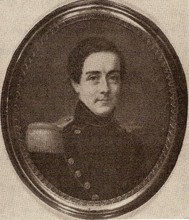
\includegraphics[scale=0.4]{images/Laurent.jpg}
\end{minipage}
&
\begin{minipage}{0.65\linewidth}
né le 18 juillet 1813 à Paris et mort le 2 septembre 1854. Polytechnicien à 19 ans, il commence une carrière militaire et participe aux expéditions de Mascart et de Tlemcen. A son retour, il fut chargé de travaux visant à l'agrandissement du port de Havre. Il exerçait son activité scientifique sur son temps libre. Il contribua en physique à la théorie des ondes et introduisit en analyse complexe le développement en série qui porte son nom. 
\end{minipage}\\
\multicolumn{2}{l}{\textbf{Brook Taylor}} \\[10pt]
\begin{minipage}{0.2\linewidth}
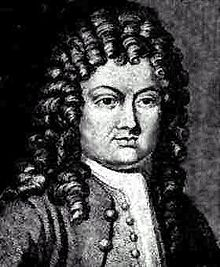
\includegraphics[scale=0.35]{images/Taylor.jpg}
\end{minipage}
&
\begin{minipage}{0.65\linewidth}
 Né à Edmonton (Londres) le 18 août 1685, et mort à Londres le 29 décembre 1731. Il invente l'intégration par parties et introduit le développement en série des applications différentiables. 
\end{minipage}
\end{tabular}

\chapter{Fonctions multiformes}
\section{L'application logarithme} 
L'application exponentielle complexe a été définie précédemment à
l'aide d'une série entière convergente dans $\mathbb{C}$. Il est
naturel de chercher une extension au plan complexe de son inverse,
l'application logarithme. Un complexe $z$ pouvant s'écrire sous la
forme $z = |z| \exp (i \theta)$ avec $\theta$ l'angle polaire associé à
$z$, on posera $log(z) = log(|z|) + i \theta$. L'application ainsi
définie ne possède malheureusement pas les bonnes propriétés que l'on
s'attendrait à obtenir. On notera en particulier qu'une discontinuité
se produit au franchissement de l'axe réel positif. Cependant, dans tout
domaine $U$ de $\mathbb{C}$ ayant une intersection nulle avec cet axe,
l'application logarithme est la fonction réciproque de l'exponentielle
complexe et est donc holomorphe dans $U$, sa dérivée étant~:
\[
log^\prime(z) = \frac{1}{z}
\]
On remarquera par ailleurs que si l'on pose de façon plus générale~:
\[
log(|z| \exp(i \theta)) = log(|z|) + i ( \theta + 2 k \pi)
\]
avec $k \in \mathbb{Z}$, l'application obtenue vérifie encore les
mêmes propriétés. On ne peut donc pas définir de façon univoque
l'application logarithme, mais ceci est possible seulement localement
(i.e. dans un domaine sans intersection avec $\mathbb{R}^+$) à
condition d'avoir fixé l'entier $k$. Par abus de langage, on appelera
application multiforme de coupure $\mathbb{R}^+$ une telle
application.
\section{Surfaces de Riemann}
Cette section est destinée à introduire un cadre formel permettant une
approche correcte des applications multiformes. Elle n'est cependant
pas nécessaire à la compréhension du reste du cours et peut être omise
en première lecture.

On rappelle qu'une application réelle ou complexe est dite analytique
sur un ouvert $U$ si elle est indéfiniment dérivable et égale à la
limite de son développement en série de Taylor en tout point de $U$. 
Soit $E$ un ensemble. On appelera carte de $E$ la donnée d'un triplet
$(U, \phi, F)$ avec $U$ partie de $E$, $F$ espace vectoriel réel ou
complexe et $\phi$ bijection de $U$ sur un ouvert de $F$. $U$ est
appelé domaine de la carte. Deux cartes $(U_1, \phi, F)$ et $(U_2,
\psi, F)$ sont compatibles si~:
\begin{itemize}
\item $\phi(U_1 \cap U_2)$ (resp. $\psi(U_1 \cap U_2)$) est un ouvert
de $F$.
\item L'application $\phi \circ \psi^{-1}$ (resp. $\psi \circ
\phi^{-1}$) de $\psi(U_1 \cap U_2)$ sur $\phi(U_1 \cap U_2)$ (resp. de
$\phi(U_1 \cap U_2)$ sur $\psi(U_1 \cap U_2)$) est analytique.
\end{itemize}
Enfin, on dira qie $E$ est une variété analytique si il existe une
famille $(U_i, \phi_i, F)_{i \in I}$ de  cartes deux à deux compatibles telle
que $\bigcup_{i \in I} U_i = E$.

Une variété analytique avec $F = \mathbb{C}$ est appelée surface de
Riemann. Une telle surface permet de généraliser la notion de graphe
d'une application. Soit en effet une application analytique $f :
\mathbb{C} \to \mathbb{C}$. La partie  $S \subset \mathbb{C}^2$ constituée des
couples de la forme $(z, f(z))$ est une surface de Riemann (prendre
comme carte l'application $\pi : \, S \to \mathbb{C}$ telle que
$\pi((z, f(z)) = z$). De façon générale, une surface de Riemann donne
localement une application analytique via les cartes, tout point de la
surface étant par définition dans le domaine d'une carte~: ceci permet
la définition des applications multiformes comme ensemble paramétré de
cartes d'une surface de Riemann. 

La figure \ref{Fi:fig4} montre partie imaginaire de  la surface de
Riemann associée à l'application $log$.
\begin{figure}[h]
\scalebox{.5}{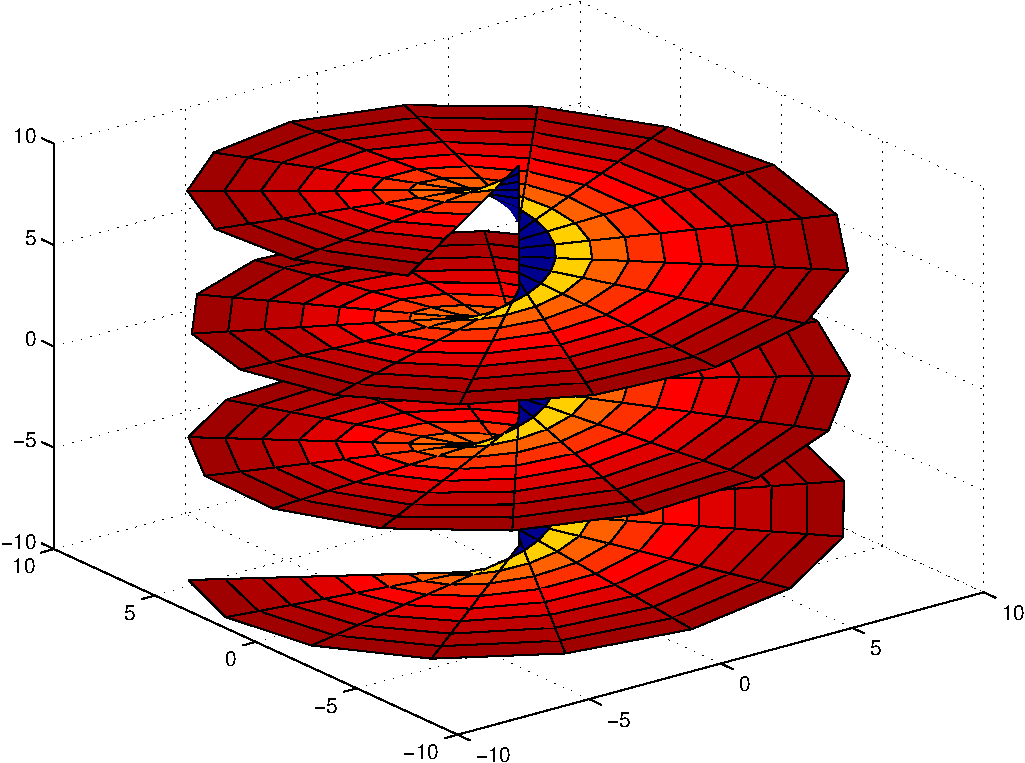
\includegraphics{images/fig4.pdf}}
\caption{Surface de Riemann de log}\label{Fi:fig4}
\end{figure}
\section{L'application racine n-ième}
Soit $n \in \mathbb{N}$.
Pour tout complexe $z = |z| \exp(i \theta)$, on pose $z^{1/n} = f_{n,k}(z) = 
|z|^{1/n} \exp i \left ( \frac{\theta+ 2 k \pi}{n}  
\right ) $ avec $k \in \mathbb{Z}$. Si l'on supprime le demi-axe réel
positif, l'application est holomorphe, sa dérivée étant~:
\[
f_{n,k}^\prime(z) = \frac{1}{n}{f_{n,k}(z)}{z}
\]

\leftline{\em Remarque}
Il est important de bien remarquer que l'on se place à $k$ fixé !

La surface de Riemann associée à la racine 3 ième est représentée
ci-dessous~:
\begin{figure}[h]
\scalebox{.5}{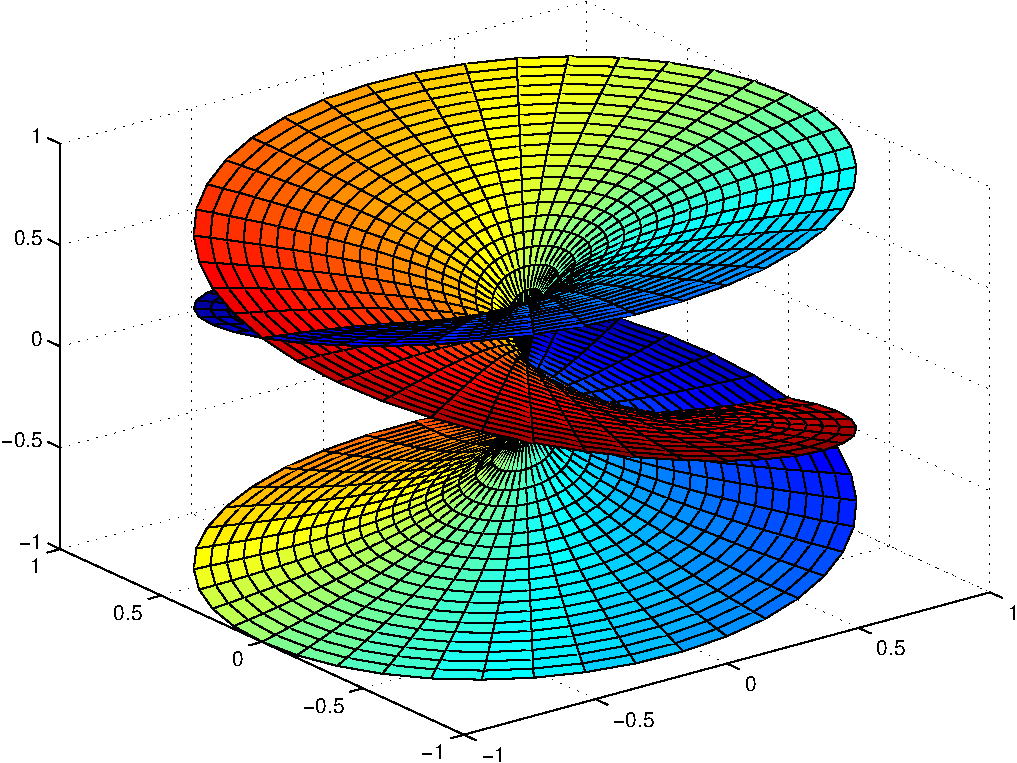
\includegraphics{images/fig5.pdf}}
\caption{Surface de Riemann de la racine 3 ième}\label{Fi:fig5}
\end{figure}
\section{L'application argument}
C'est l'application $f_k$ qui à $z = |z| \exp (i \theta)$ associe
$\theta + k 2 ^pi$. Ce n'est pas à proprement parler une application
multiforme, sa partie imaginaire étant nulle. On remarque par ailleurs
que cette application est simplement la partie imaginaire du
logarithme complexe. Par extension, on lui associera néanmoins une
surface de représentation dans $\mathbb{R^3}$~:
\begin{figure}[h]
\scalebox{.5}{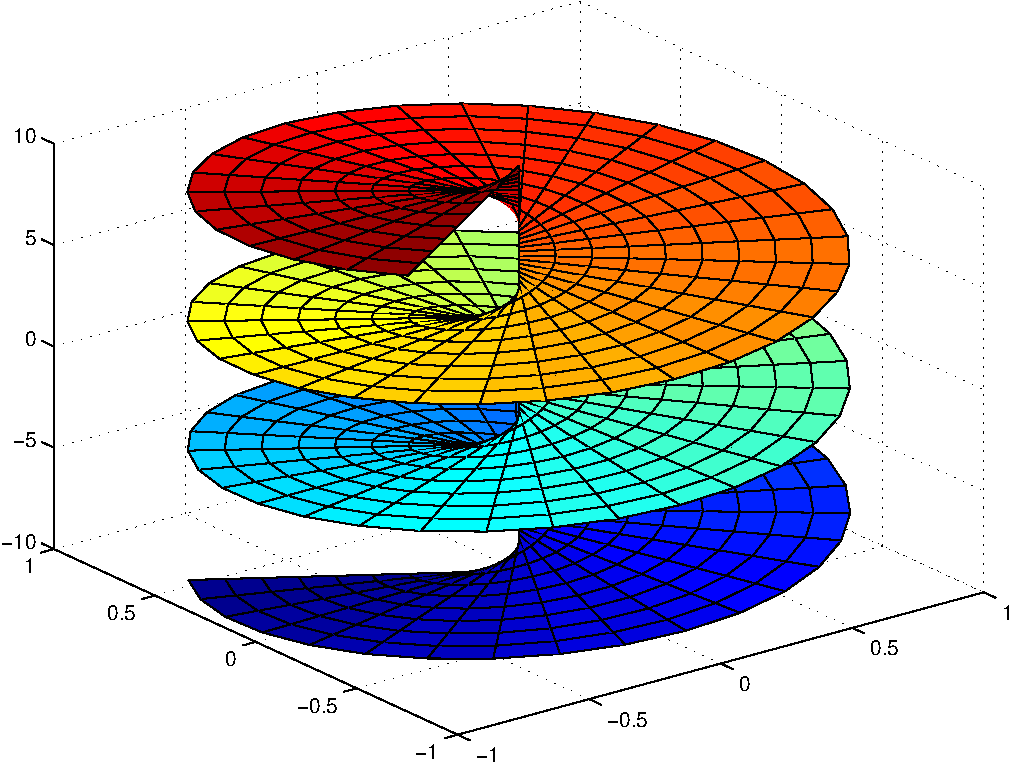
\includegraphics{images/fig3.pdf}}
\caption{Surface de représentation de arg}\label{Fi:fig3}
\end{figure}
\begin{exercice}
Calculer les intégrales~:
\[
I_1 = \int_0^{+\infty} \frac{x^2-1}{(x^2+1)^2}ln(x)dx
\]
\[
I_2 = \int_0^{+\infty} \frac{x^{a-1}}{1+x}dx, \, a \in ]0, 1[
\]
\end{exercice}
\chapter{Transformation de Laplace}
\section{Définition}
Soit $f : \mathbb{R} \to \mathbb{C}$ une application telle que~:
\begin{itemize}
\item $\forall t < 0, \, f(t) = 0$.
\item $f$ est intégrable sur tout compact de $\mathbb{R}$.
\item Il existe un réel $x$ tel que l'intégrale~:
\[
\int_{\mathbb{R}^+}e^{-xt} f(t) dt
\]
soit convergente.
\end{itemize}
\begin{mandatory}
\begin{defn}
Soit $f$ une application vérifiant les conditions précédentes. La
transformée de Laplace de $f$ est l'application $\mathcal{L}(f) : \Omega \subset \mathbb{C} \to
\mathbb{C}$ définie par~:
\[
\mathcal{L}(f)(p) = \int_0^{+\infty}e^{-pt} f(t) dt
\]
$\Omega$ étant l'ensemble des $p$ pour lesquels l'intégrale précédente
est définie.
\end{defn}
\end{mandatory}
\begin{mandatory}
\begin{prop}
Si la transformation de Laplace de $f$ est définie pour $p_0$, elle
est également définie pour tout $p$ tel que $\Re(p) > \Re(p_0)$.
\end{prop} 
\end{mandatory}
La borne inférieure de l'ensemble des $x$ pour lesquels l'intégrale de
Laplace est convergente pour $\Re(p) = x$ est appelée abscisse de
convergence de la transformation de Laplace.
On définira de même l'abscisse de convergence absolue, qui est
supérieure ou égale à l'abscisse de convergence. On remarquera que
chacune de ces bornes peut être $-\infty$.
\begin{mandatory}
\begin{prop}
Soit $p_0$ un complexe tel que la transformée de Laplace $\mathcal{L}(f)(p_0)$ de
$f$ soit définie. Soit $C_{\alpha, p_0}$ l'ensemble des complexes de
la forme $p_0 + r e^{i \theta}$ avec $r \in \mathbb{R}^+$ et $\theta
\in [-\alpha, \alpha]$. L'intégrale de Laplace est uniformément
convergente dans $C_{\alpha, p_0}$ si $\alpha \in ]0, \frac{\pi}{2}[$.
\end{prop}
\end{mandatory}
\begin{proof}
Soit $\epsilon > 0$ et soit $T > 0$ tel que pour tout $t > T$~:
\[
\int_T^t e^{-p_0 u}f(u) du < \epsilon
\]
On note $g(t) = \int_T^t e^{-p_0 u}f(u) du$.
Posons $p = p_0 + h$ pour $p \in C_{\alpha, p_0}$ et $h = r e^{i
\theta}$. On a~:
\[
\int_T^t e^{-p u}f(u) du = \int_T^t e^{-hu}g^\prime(u) du
\]
Une intégration par parties conduit à~:
\[
\int_T^t e^{-hu}g^\prime(u) dt = e^{-ht}g(t) + h \int_T^t e^{-hu}g(u) du
\]
Pour $t > T$ le premier terme est inférieur à $\epsilon$, alors que le
second est borné en module par~:
\[
r \epsilon \int_T^{+\infty} e^{-r u \cos(\alpha)} d u =
\frac{\epsilon}{\cos(\alpha)} 
\]
\end{proof}
La transformation de Laplace est holomorphe dans son domaine de
convergence comme le montre la proposition suivante.
\begin{mandatory}
\begin{prop}
Soit $f$ continue sur $\mathbb{R}^+$ et soit $s$ l'abscisse de
convergence de sa transforméee de Laplace $F$. Alors $F$ est
holomorphe dans le demi-plan complexe formé des points de partie
réelle strictement supérieure à $s$.
\end{prop}
\end{mandatory}
\begin{proof}
Soit $p = x+iy$ avec $x > s$. Soit $p_0 = x_0 + i y$ un point tel
que $s < x_0 < x$. Pour tout $\alpha \in ]0, \frac{\pi}{2}[$, le point
$p$ appartient à $C_{\alpha, p_0}$ et l'intégrale définissant $F$
est uniformément convergente dans $C_{\alpha, p_0}$. De plus,
l'application~:
\[
p \to e^{-pt} f(t)
\]
est indéfiniment dérivable sur $C_{\alpha, p_0}$ et $t > 0$. On en
déduit alors (dérivation sous le signe somme) que $F(p)$ est
holomorphe dans $C_{\alpha, p_0}$ et que~:
\[
F^{(n)}(p) = (-1)^n \int_0^{+\infty} t^n f(t) e^{-pt} dt
\] 
\end{proof}
\begin{rem}
La proposition reste vraie si $f$ est seulement continue par morceaux.
\end{rem}
\section{Propriétés}
La transformation de Laplace est de façon évidente linéaire. Son
intérêt principal vient de son comportement vis à vis de la
dérivation.
\begin{mandatory}
\begin{prop}
Soit $f$ continue sur $\mathbb{R}^+$, dérivable. Si elle admet une
transformée de laplcace ainsi que sa dérivée, les deux transformées
sont liées par la relation~:
\[
\mathcal{L}(f^\prime)(p) = p \mathcal{L}(f)(p) - f(0^+)
\] 
avec $f(0^+) = \lim_{ t \to 0, t > 0} f(t)$
\end{prop}
\end{mandatory}
\begin{proof}
On a~:
\[
\mathcal{L}(f^\prime)(p) = \lim_{t\to + \infty} \int_0^Tf^\prime(t) e^{-pt} dt
\]
Une intégration par parties montre que l'intégrale de droite vaut~:
\[
\left [
e^{-pt}f(t)
\right ]_0^T
+ p \int_0^T f(t) e^{-pt} dt
\]
Qui montre la proposition par passage à la limite.
\end{proof}
Cette proposition s'étend par récurrence pour les dérivées d'ordre
quelconque~:
\[
\mathcal{L}(f^{(n)})(p) = p^n \mathcal{L}(f)(p) - p^{n-1} f(0)
- p^{n-2} f^\prime(0) - \dots f^{(n-1)}(O^+))
\]
Il est possible de déterminer également la transformée de Laplace de
la primitive d'une application.
\begin{mandatory}
\begin{prop}
Si $f$ admet une transformée de Laplace $F$ et si $\lim_{t \to 0^+}
\frac{f(t)}{t}$ existe, alors~:
\[
\mathcal{L}(f(t)/t)(p) = \int_p^{+\infty} F(u) du
\]
\end{prop} 
\end{mandatory}
\begin{proof}
\[
\int_p^Z F(u) du = \int_p^Z \int_0^{+\infty} e^{-ut}
f(t) dt du
\]
comme l'intégrale de Laplace est uniformément convergente dans un
secteur angulaire, on peut intervertir l'ordre de intégrations et
l'intégrale devient~:
\[
\int_0^{+\infty} e^{-pt} \frac{f(t)}{t} dt - \int_0^{+\infty} e^{-Zt} \frac{f(t)}{t} dt
\] 
La conclusion s'obtient en faisant tendre $Z$ vers l'infini en module.
\end{proof}
\begin{mandatory}
\begin{prop}
Soit $f$ de transformée de Laplace $F$ et soit $s$ l'abscisse de
convergence de cette transformée. Alors l'application~:
\[
\int_0^t f(u) du
\]
admet pour transformée de Laplace $\frac{F(p)}{p}$ et son abscisse de
convergence est strictement supérieure à $\sup(0, s)$.
\end{prop}
\end{mandatory}
Cette proposition se montre de façon similaire à la précédente.
\begin{prop}
Soit $f$ admettant une transformée de Laplace $F$ d'abscisse de
convergence $s$. Soit $a \in \mathbb{C}$. Alors l'application
$e^{at}f(t)$ admet pour transformée de Laplace $F(p-a)$, son abscisse
de convergence étant $s + \Re(a)$.
\end{prop}
\begin{prop}
Soit $f$ admettant $F$ pour transformée de Laplace. Soit $a \in
\mathbb{R}$. Alors
l'application $g$ telle que $g(t) = 0$ si $t < a$ et $g(t) = f(t-a)$
sinon admet pour transforméee de Laplace $e^{-ap}F(p)$.
\end{prop}
Ces deux propositions se montrent de manière immédiate.
On peut calculer facilement à partir de ceci la transformée de Laplace
d'une application périodique. Soit $f_1$ une application à support
dans un intervalle réel $[0,T]$ et soit $f$ l'application définie par
périodisation de $f_1$ de période $T$. Si $f$ admet une transformée de
Laplace et si $F_1$ est la transformée de Laplace de $f_1$, alors~:
\[
\mathcal{L}(f)(p) = \frac{F_1(p)}{1-e^{-pT}}
\]
Ce résultat s'obtient en écrivant $f$ sous la forme d'une somme de
termes de la forme $f_1(t-k T)$ avec $k \in \mathbb{N}$ et en faisant
apparaître une série géométrique.
On a enfin une proposition relative aux changements d'échelle.
\begin{prop}
Si $f$ admet pour transformée de Laplace $F$ alors, pour $\lambda \in
\mathbb{R^*}$, l'application $f(t/\lambda)$ admet pour transformée de
Laplace $\lambda F(\lambda p)$
\end{prop}
\section{Inversion}
\begin{mandatory}
\begin{prop}(Théorème de la valeur finale)
Soit $f$ continue de transformée de Laplace $F$. Si l'abscisse de convergence
$s$ est négative, alors~:
\[
\lim_{p \to O^+} p F(p) = \lim_{t \to +\infty} f(t)
\]
\end{prop}
\end{mandatory}
\begin{proof}
Soit $l = \lim_{t \to +\infty} f(t)$. 
\begin{align*}
pF(p) - l & = p \int_0^{+\infty} e^{-pt}f(t) dt - l \\
&= p \int_0^T  e^{-pt}f(t) dt + p  \int_T^{+\infty}e^{-pt}(f(t) -l) dt
\\ &+ l \left (
p \int_T^{+\infty} e^{-pt}dt -1
\right )
\end{align*}
Le premier terme est majoré en module par~:
\[
|p| T M_T
\]
avec $M_T$ borne sup de $|f|$ sur $[0,T]$.
Le second terme se majore uniformément par définition de la limite de
$f$ en $+\infty$ et la convergence uniforme de l'intégrale. Enfin, le
troisième terme tend vers 0 pour $|p|\to O^+|$, ce qui montre la proposition.
\end{proof}
\begin{mandatory}
\begin{prop}(Théorème de la valeur initiale)
Soit $f$ dérivable, de transforméee de Laplace $F$ et telle que sa
dérivée soit également transformable. Alors~:
\[
\lim_{|p|\to +\infty} p F(p) = f(0^+)
\]
\end{prop}
\end{mandatory}
\begin{proof}
On a~:
\[
\lim_{|p| \to +\infty} \mathcal{L}(f^\prime)(p) = 0
\]
et $\mathcal{L}(f^\prime)(p) = p F(p) - f(0^+)$.
\end{proof}
\begin{mandatory}
\begin{prop}
Soit $f$ définie par une série entiére convergente $\sum_{n \in
\mathbb{N}} a_n t^n / n!$ de rayon de convergence infini. Alors elle
est transformable et sa transformée s'obtient en transformant terme à terme.
\end{prop}
\end{mandatory}
\begin{defn}
Soit $[a,b]$ un intervalle de $\mathbb{R}$. Soit $f : [a,b] \to \mathbb{R} (\mbox{ resp. } \mathbb{C})$. On dira
que $f$ est à variation bornée si~:
\[
\sup \{ \sum_{i=0\dots N-1} |f(t_{i+1}) - f(t_i)|, \, a = t_0 < t_1, \dots < t_N = b, \, N \in \mathbb{N} \} < + \infty
\]
\end{defn}
La définition précédente s'étend immédiatement au cas des intervalles semi-infinis ou infinis.
La proposition suivant est trés classique~:
\begin{prop}(Lemme de Dirichlet)
Soit $f$ à variation bornée sur un intervalle $[0,a]$. On a~:
\[
\lim_{b \to +\infty} \int_[0,a] f(x) \frac{\sin bx}{x} d \lambda(x) =
f(0^+) \lim_{T \to +\infty} \int_[0,T] \frac{\sin x}{x} d \lambda(x)  
\]
\end{prop}
\begin{mandatory}
\begin{theorem}
Soit $F$ la transformée de Laplace d'une application à variation bornée $f$, l'abscisse
de convergence étant $s$. En tout point de continuité $t$ de $f$, on a~:
\[
f(t) = \frac{1}{i 2 \pi} \lim_{b \to + \infty} \int_{a-ib}^{a+ib}
e^{pt} F(p) dp
\]
avec $a > s$.
\end{theorem}
\end{mandatory}
\begin{proof}
Formons~:
\[
f_b(t) = \frac{1}{i 2 \pi}  \int_{a-ib}^{a+ib} e^{pt} \int_0^{\infty}
e^{-pu} f(u) du dp
\]
La convergence de l'intégrale étant uniforme, on peut écrire, après
interversion des intégrales~:
\[
f_b(t) = \frac{1}{\pi} e^{at} \int_{-t}^{+\infty} f(u+t)e^{-a(u+t)}
\frac{sin b u}{u} du
\]
Comme par ailleurs $f(t) = 0, \, t < 0$, on a~:
\[
f_b(t) = \frac{1}{\pi} e^{at} \int_{-\infty}^{+\infty} f(u+t)e^{-a(u+t)}
\frac{sin b u}{u} du
\]
Soit encore~:
\[
f_b(t) = \frac{1}{\pi} e^{at} \int_{0}^{+\infty} \left (
f(u+t)e^{-a(u+t)} + f(t-u)e^{-a(t-u)}
\right )
\frac{sin b u}{u} du
\]
En utilisant~:
\[
\int_0^{+\infty} \frac{sin b u}{u} du = \frac{\pi}{2}
\]
On obtient~:
\[
f_b(t) = f(t)  + \frac{1}{\pi} e^{at} \int_{0}^{+\infty} \left (
f(u+t)e^{-a(u+t)} + f(t-u)e^{-a(t-u)} - 2 f(t)e^{-at}
\right )
\frac{sin b u}{u} du
\]
Le résultat s'obtient alors en faisant tendre $b$ vers $+\infty$ et en utilisant le lemme de Dirichlet.
\end{proof} 
Il existe une forme réciproque de ce théorème~:
\begin{mandatory}
\begin{theorem}
Soit une application $F$ analytique dans un demi-plan $\Re(p) > s_0$,
tendant vers 0 pour $|p| \to +\infty$ dans tout demi-plan $\Re(p) > s
> s_0$. Si l'intégrale~:
\[
\int_{s-i \infty}^{s+i \infty} F(p) dp
\]
converge absolument pour $s > s_0$, alors $F$ est la transformée de
Laplace de l'application $f$ définie par~:
\[
f(t) = \frac{1}{i 2 \pi} \int_{s-i \infty}^{s+i \infty} F(p) dp
\]
\end{theorem}
\end{mandatory}
\begin{exercice}
Déterminer l'original de l'application~:
\[
F : p \to \frac{1}{1+p^3}
\]
en utilisant~:
\begin{itemize}
\item Les originaux élémentaires.
\item La formule d'inversion de Mellin-Fourier.
\end{itemize}
\end{exercice}
\end{document}
